%% ----------------------------------------------------------------
%% Thesis.tex -- MAIN FILE (the one that you compile with LaTeX)
%% ---------------------------------------------------------------- 

% Set up the document
\documentclass[a4paper, 11pt, oneside]{Thesis}  % Use the "Thesis" style, based on the ECS Thesis style by Steve Gunn
\graphicspath{Images/}  % Location of the graphics files (set up for graphics to be in PDF format)

% Include any extra LaTeX packages required
\usepackage[square, numbers, comma, sort&compress]{natbib}  % Use the "Natbib" style for the references in the Bibliography
\usepackage{verbatim}  % Needed for the "comment" environment to make LaTeX comments
\usepackage{vector}  % Allows "\bvec{}" and "\buvec{}" for "blackboard" style bold vectors in maths
\hypersetup{urlcolor=blue, colorlinks=true}  % Colours hyperlinks in blue, but this can be distracting if there are many links.
\usepackage{float}
\usepackage{times}
\usepackage{graphicx} % more modern
\usepackage{subfigure}
%\usepackage{natbib}
\usepackage{amsmath}
\usepackage{enumerate}
%\usepackage{bbm}
\usepackage{makecell}
%\usepackage{booktabs}
\usepackage{tabularx}
\usepackage{multirow, bm, threeparttable}
\usepackage[usenames,dvipsnames,table]{xcolor}
\usepackage{csvsimple}
\usepackage{siunitx}
\usepackage{bbm}
\usepackage{bibentry}
%\usepackage{ulem}
%\usepackage{pdfpages}
%\usepackage{fullpage}
\usepackage{changes}
\newcolumntype{R}{>{$}r<{$}}
\newcolumntype{L}{>{$}l<{$}}
\newcolumntype{M}{R@{${}={}$}L}
\usepackage{multirow}


% math
\DeclareMathOperator*{\Mean}{Mean}
\DeclareMathOperator*{\Median}{Median}

% For algorithms
\usepackage{algorithm}
\usepackage{algorithmic}
\usepackage{hyperref}
\renewcommand{\thefigure}{A\arabic{figure}}
\renewcommand{\thetable}{A\arabic{table}}

\usepackage{pdflscape}
\usepackage{afterpage}
\usepackage{capt-of}
% other
\renewcommand\thesection{\Alph{section}}

%\newcommand{\theHalgorithm}{\arabic{algorithm}}

\newcommand{\tabincell}[2]{\begin{tabular}{@{}#1@{}}#2\end{tabular}}

\renewcommand{\thetable}{S\arabic{table}}
%% ----------------------------------------------------------------
\begin{document}
\frontmatter      % Begin Roman style (i, ii, iii, iv...) page numbering

% Set up the Title Page
\title  {Molecular Machine Learning with DeepChem}
\authors  {\texorpdfstring
            {\href{https://rbharath.github.io}{Bharath Ramsundar}}
            {Bharath Ramsundar}
            }
\addresses  {\groupname\\\deptname\\\univname}  % Do not change this here, instead these must be set in the "Thesis.cls" file, please look through it instead
\date       {\today}
%\subject    {}
%\keywords   {}

\maketitle
%% ----------------------------------------------------------------

\setstretch{1.3}  % It is better to have smaller font and larger line spacing than the other way round

% Define the page headers using the FancyHdr package and set up for one-sided printing
\fancyhead{}  % Clears all page headers and footers
\rhead{\thepage}  % Sets the right side header to show the page number
\lhead{}  % Clears the left side page header

\pagestyle{fancy}  % Finally, use the "fancy" page style to implement the FancyHdr headers

%% ----------------------------------------------------------------
% Declaration Page required for the Thesis, your institution may give you a different text to place here
\Declaration{

\addtocontents{toc}{\vspace{1em}}  % Add a gap in the Contents, for aesthetics

I, Bharath Ramsundar, declare that this thesis titled, `Molecular Machine Learning with DeepChem' and the work presented in it are my own. I confirm that:

\begin{itemize} 
\item[\tiny{$\blacksquare$}] This work was done wholly or mainly while in candidature for a research degree at this University.
 
\item[\tiny{$\blacksquare$}] Where any part of this thesis has previously been submitted for a degree or any other qualification at this University or any other institution, this has been clearly stated.
 
\item[\tiny{$\blacksquare$}] Where I have consulted the published work of others, this is always clearly attributed.
 
\item[\tiny{$\blacksquare$}] Where I have quoted from the work of others, the source is always given. With the exception of such quotations, this thesis is entirely my own work.
 
\item[\tiny{$\blacksquare$}] I have acknowledged all main sources of help.
 
\item[\tiny{$\blacksquare$}] Where the thesis is based on work done by myself jointly with others, I have made clear exactly what was done by others and what I have contributed myself.
\\
\end{itemize}
 
 
Signed:\\
\rule[1em]{25em}{0.5pt}  % This prints a line for the signature
 
Date:\\
\rule[1em]{25em}{0.5pt}  % This prints a line to write the date
}
\clearpage  % Declaration ended, now start a new page

%% ----------------------------------------------------------------
% The "Funny Quote Page"
%\pagestyle{empty}  % No headers or footers for the following %pages

%\null\vfill
%% Now comes the "Funny Quote", written in italics
%\textit{``Write a funny quote here.''}

%\begin{flushright}
%If the quote is taken from someone, their name goes here
%\end{flushright}

%\vfill\vfill\vfill\vfill\vfill\vfill\null
%\clearpage  % Funny Quote page ended, start a new page
%% ----------------------------------------------------------------

% The Abstract Page
\addtotoc{Abstract}  % Add the "Abstract" page entry to the Contents
\abstract{
\addtocontents{toc}{\vspace{1em}}  % Add a gap in the Contents, for aesthetics


Machine learning has widely been applied to image, video, and
speech datasets, but has not yet achieved broad penetration into
chemistry, materials science, or other molecular design applications. However, over the last few years, machine learning and deep learning have achieved notable successes in predicting properties of molecular systems. In this thesis, I present a series of deep learning algorithms that demonstrate strong predictive improvements across a wide range of biochemical tasks such as assay activity modeling, toxicity prediction, protein-ligand binding affinity calculation, and chemical retrosynthesis. In addition to these algorithmic improvements, I introduce the comprehensive benchmark suite MoleculeNet for molecular machine learning algorithms (https://moleculenet.ai) and demonstrate how the technology of one-shot learning can be used for drug discovery applications. The work presented in this thesis culminated in my design and construction of DeepChem (https://deepchem.io), an open source package for molecular machine learning, which has achieved broad adoption among biotech startups, pharmaceutical companies, and research groups. DeepChem has attracted a thriving community of open source developers and looks to continue growing and expanding as a vibrant research tool. 
}

\clearpage  % Abstract ended, start a new page
%% ----------------------------------------------------------------

\setstretch{1.3}  % Reset the line-spacing to 1.3 for body text (if it has changed)

% The Acknowledgements page, for thanking everyone
\acknowledgements{
\addtocontents{toc}{\vspace{1em}}  % Add a gap in the Contents, for aesthetics

My thanks to the computer science department at Stanford for taking a chance on a student who'd previously spent more time working on math than on computers.

My thanks to Robert McGibbon for my initial introduction to computational chemistry. To Steven Kearnes for teaching me about computational drug discovery. To David Konerding for letting me take on a crazy internship project at Google working on drug discovery. To Patrick Riley and the GAS team at Google for giving me the opportunity to continue exploring deep learning and drug discovery at Google. To Evan Feinberg for explaining and exploring protein binding with me. To Joe Gomes for teaching me some quantum chemistry and force field design. To Michael Wu for working with me on a small benchmarking project that grew into a multiyear effort. To Bowen Liu for helping me understand chemical synthesis. To Aneesh Pappu for being a great summer intern. To Prasad Kawthekar for exploring the DeepChem GUI and synthesis with me.

My thanks to my industrial collaborators from pharma, Denny Rajiah, Govindan Subramanian, Robert Sheridan, Andreas Verras, and Matthew Tudor for taking a chance on experimenting with untested machine learning methods.

I'd especially like to acknowledge the entire DeepChem development team. It's your efforts that have transformed a few scripts on GitHub into a thriving open source project and community. Special thanks to Peter Eastman, Karl Leswing, and Michael Wu for all the time they've put in. More generally, my heartfelt thanks to our users and supporters for putting up with the limitations of our software and working with us to improve it.

My thanks to my computer science co-advisor Leo Guibas for letting me spend all my time working on problems in biology and chemistry.

Finally, my heartfelt thanks to Vijay Pande for letting me spend years exploring the applications of deep learning to chemistry, biology, physics and more. Senior scientists who create a safe space for beginners to explore novel ideas are invaluable, and Vijay was brilliant in letting us explore crazy ideas while providing constant support.


}
\clearpage  % End of the Acknowledgements
%% ----------------------------------------------------------------

\pagestyle{fancy}  %The page style headers have been "empty" all this time, now use the "fancy" headers as defined before to bring them back


%% ----------------------------------------------------------------
\lhead{\emph{Contents}}  % Set the left side page header to "Contents"
\tableofcontents  % Write out the Table of Contents

%% ----------------------------------------------------------------
\lhead{\emph{List of Figures}}  % Set the left side page header to "List if Figures"
\listoffigures  % Write out the List of Figures

%% ----------------------------------------------------------------
\lhead{\emph{Molecular Machine Learning with DeepChem}}  % Set the left side page header to "List of Tables"
\listoftables  % Write out the List of Tables

%% ----------------------------------------------------------------
--
% End of the pre-able, contents and lists of things
% Begin the Dedication page

\setstretch{1.3}  % Return the line spacing back to 1.3

\pagestyle{empty}  % Page style needs to be empty for this page
\dedicatory{Dedicated to my family for their unstinting love, encouragement, and support}

\addtocontents{toc}{\vspace{2em}}  % Add a gap in the Contents, for aesthetics


%% ----------------------------------------------------------------
\mainmatter	  % Begin normal, numeric (1,2,3...) page numbering
\pagestyle{fancy}  % Return the page headers back to the "fancy" style

% Include the chapters of the thesis, as separate files
% Just uncomment the lines as you write the chapters
%\clearpage
%%\documentclass{article}
%\normalem


%\begin{document}

\section{Massively Multitask Networks for Drug Discovery}
%\author{Bharath Ramsundar*, Steven Kearnes*\\Patrick Riley, Dale Webster,
%David Konerding\\Vijay Pande\\(*Equal contribution.)}

%\twocolumn[\maketitle]

\subsection{Abstract}
Massively multitask neural architectures provide a learning framework for
drug discovery that synthesizes information from many distinct biological
sources. To train these architectures at scale, we gather large amounts of
data from public sources to create a dataset of nearly 40 million
measurements across more than 200 biological targets. We investigate
several aspects of the multitask framework by performing a series of
empirical studies and obtain some interesting results: $(1)$ massively
multitask networks obtain predictive accuracies significantly better than
single-task methods, $(2)$ the predictive power of multitask networks
improves as additional tasks and data are added, $(3)$ the total amount of
data and the total number of tasks both contribute significantly to
multitask improvement, and $(4)$ multitask networks afford limited
transferability to tasks not in the training set. Our results underscore
the need for greater data sharing and further algorithmic innovation to
accelerate the drug discovery process.


\subsection{Introduction}
\label{intro}

Discovering new treatments for human diseases is an immensely complicated
challenge. Prospective drugs must attack the source of an illness, but must
do so while satisfying restrictive metabolic and toxicity constraints.
Traditionally, drug discovery is an extended process that takes years to
move from start to finish, with high rates of failure along the way.

After a suitable target has been identified, the first step in the drug
discovery process is ``hit finding.'' Given some druggable target,
pharmaceutical companies will screen millions of drug-like compounds in an
effort to find a few attractive molecules for further optimization. These
screens are often automated via robots, but are expensive to perform.
Virtual screening attempts to replace or augment the high-throughput
screening process by the use of computational methods
\cite{shoichet2004virtual}. Machine learning methods have frequently been
applied to virtual screening by training supervised classifiers to predict
interactions between targets and small molecules.

There are a variety of challenges that must be overcome to achieve
effective virtual screening. Low hit rates in experimental screens (often
only $1$--$2$\% of screened compounds are active against a given target)
result in imbalanced datasets that require special handling for effective
learning. For instance, care must be taken to guard against unrealistic
divisions between active and inactive compounds (``artificial enrichment'')
and against information leakage due to strong similarity between active
compounds (``analog bias'') \cite{rohrer2009maximum}.  Furthermore, the
paucity of experimental data means that overfitting is a perennial thorn.

The overall complexity of the virtual screening problem has limited the
impact of machine learning in drug discovery. To achieve greater predictive
power, learning algorithms must combine disparate sources of experimental
data across multiple targets. Deep learning provides a flexible paradigm
for synthesizing large amounts of data into predictive models. In
particular, multitask networks facilitate information sharing across
different experiments and compensate for the limited data associated with
any particular experiment.

In this work, we investigate several aspects of the multitask learning
paradigm as applied to virtual screening. We gather a large collection of
datasets containing nearly 40 million experimental measurements for over
200 targets. We demonstrate that multitask networks trained on this
collection achieve significant improvements over baseline machine learning
methods. We show that adding more tasks and more data yields better
performance. This effect diminishes as more data and tasks are added, but
does not appear to plateau within our collection. Interestingly, we find
that the total amount of data and the total number of tasks both have
significant roles in this improvement. Furthermore, the features extracted
by the multitask networks demonstrate some transferability to tasks not
contained in the training set. Finally, we find that the presence of shared
active compounds is moderately correlated with multitask improvement, but
the biological class of the target is not.

\subsection{Related Works}

Machine learning has a rich history in drug discovery. Early work combined
creative featurizations of molecules with off-the-shelf learning algorithms
to predict drug activity \cite{varnek2012machine}. The state of the art has
moved to more refined models, such as the influence relevance voting method
that combines low-complexity neural networks and k-nearest neighbors
\cite{swamidass2009influence}, and Bayesian belief networks that repurpose
textual information retrieval methods for virtual screening
\cite{abdo2010ligand}. Other related work uses deep recursive neural
networks to predict aqueous solubility by extracting features from the
connectivity graphs of small molecules \cite{lusci2013deep}.

Deep learning has made inroads into drug discovery in recent years, most
notably in 2012 with the Merck Kaggle competition \cite{dahl2012deep}.
Teams were given pre-computed molecular descriptors for compounds with
experimentally measured activity against 15 targets and were asked to
predict the activity of molecules in a held-out test set. The winning team
used ensemble models including multitask deep neural networks, Gaussian
process regression, and dropout to improve the baseline test set $R^2$ by
nearly 17\%. The winners of this contest later released a technical report
that discusses the use of multitask networks for virtual screening
\cite{dahl2014multi}. Additional work at Merck analyzed the choice of
hyperparameters when training single- and multitask networks and showed
improvement over random forest models \cite{ma2015deep}. The Merck Kaggle
result has been received with skepticism by some in the cheminformatics and
drug discovery communities \citep[and associated comments]{lowe2012did}.
Two major concerns raised were that the sample size was too small (a good
result across 15 systems may well have occurred by chance) and that any
gains in predictive accuracy were too small to justify the increase in
complexity.

While we were preparing this work, a workshop paper was released that also
used massively multitask networks for virtual screening
\cite{unterthinerdeep}. That work curated a dataset of 1,280 biological
targets with 2 million associated data points and trained a multitask
network. Their network has more tasks than ours (1,280 vs. 259) but far
fewer data points (2 million vs. nearly 40 million). The emphasis of our
work is considerably different; while their report highlights the
performance gains due to multitask networks, ours is focused on
disentangling the underlying causes of these improvements. Another closely
related work proposed the use of collaborative filtering for virtual
screening and employed both multitask networks and kernel-based methods
\cite{erhan2006collaborative}. Their multitask networks, however, did not
consistently outperform single-task models.

Within the greater context of deep learning, we draw upon various strands
of recent thought. Prior work has used multitask deep networks in the
contexts of language understanding \cite{collobert2008unified} and
multi-language speech recognition \cite{deng2013new}. Our best-performing
networks draw upon design patterns introduced by GoogLeNet
\cite{szegedy2014going}, the winner of ILSVRC 2014.

\subsection{Methods}

\subsubsection{Dataset Construction and Design}
\label{sec:datasets}
Models were trained on $259$ datasets gathered from publicly available
data.  These datasets were divided into four groups: PCBA, MUV, DUD-E, and
Tox21.  The PCBA group contained $128$ experiments in the PubChem BioAssay
database \cite{wang2012pubchem}.  The MUV group contained $17$ challenging
datasets specifically designed to avoid common pitfalls in virtual
screening \cite{rohrer2009maximum}. The DUD-E group contained $102$
datasets that were designed for the evaluation of methods to predict
interactions between proteins and small molecules
\cite{mysinger2012directory}.  The Tox21 datasets were used in the recent
Tox21 Data Challenge (\url{https://tripod.nih.gov/tox21/challenge/}) and
contained experimental data for $12$ targets relevant to drug toxicity
prediction. We used only the training data from this challenge because the
test set had not been released when we constructed our collection.  In
total, our $259$ datasets contained $37.8$M experimental data points for
$1.6$M compounds. Details for the dataset groups are given in
\tablename~\ref{tab:datasets}. See the Appendix for details on individual
datasets and their biological target categorization.

\begin{table}
\small
\centering
\caption{Details for dataset groups. Values for the number of data points
per dataset and the percentage of active compounds are reported as means,
with standard deviations in parenthesis.}
\vskip 0.2 in
\label{tab:datasets}
\begin{tabular}{llll}
\toprule
{Group} & {Datasets} & {Data Points / ea.} & {\% Active} \\
\midrule
{PCBA} & 128 & $282\text{K}$ $(122\text{K})$ & $1.8$ $(3.8)$ \\
DUD-E & $102$ & $14\text{K}$ $(11\text{K})$ & $1.6$ $(0.2)$ \\
MUV & $17$ & $15\text{K}$ $(1)$ & $0.2$ $(0)$ \\
Tox21 & $12$ & $6\text{K}$ $(500)$ & $7.8$ $(4.7)$ \\
\bottomrule
\end{tabular}
\vskip -0.2in
\end{table}

It should be noted that we did not perform any preprocessing of our
datasets, such as removing potential experimental artifacts. Such artifacts
may be due by compounds whose physical properties cause interference with
experimental measurements or allow for promiscuous interactions with many
targets. A notable exception is the MUV group, which has been processed
with consideration of these pathologies \cite{rohrer2009maximum}.

\subsubsection{Small Molecule Featurization}
We used extended connectivity fingerprints (ECFP4)
\cite{rogers2010extended} generated by RDKit \cite{landrumrdkit} to
featurize each molecule. The molecule is decomposed into a set of
fragments---each centered at a non-hydrogen atom---where each fragment
extends radially along bonds to neighboring atoms. Each fragment is
assigned a unique identifier, and the collection of identifiers for a
molecule is hashed into a fixed-length bit vector to construct the
molecular ``fingerprint''.  ECFP4 and other fingerprints are commonly used
in cheminformatics applications, especially to measure similarity between
compounds \cite{willett1998chemical}. A number of molecules (especially in
the Tox21 group) failed the featurization process and were not used in
training our networks. See the Appendix for details.

\subsubsection{Validation Scheme and Metrics}

The traditional approach for model evaluation is to have fixed training,
validation, and test sets.  However, the imbalance present in our datasets
means that performance varies widely depending on the particular
training/test split. To compensate for this variability, we used stratified
$K$-fold cross-validation; that is, each fold maintains the active/inactive
proportion present in the unsplit data. For the remainder of the paper, we
use $K=5$.

Note that we did not choose an explicit validation set. Several datasets in
our collection have very few actives ($\sim30$ each for the MUV group), and
we feared that selecting a specific validation set would skew our results.
As a consequence, we suspect that our choice of hyperparameters may be
affected by information leakage across folds. However, our networks do not
appear to be highly sensitive to hyperparameter choice (see
Section~\ref{sec:experimental}), so we do not consider leakage to be a
serious issue.

Following recommendations from the cheminformatics community
\cite{jain2008recommendations}, we used metrics derived from the receiver
operating characteristic (ROC) curve to evaluate model performance. Recall
that the ROC curve for a binary classifier is the plot of true positive
rate (TPR) vs. false positive rate (FPR) as the discrimination threshold is
varied.  For individual datasets, we are interested in the area under the
ROC curve (AUC), which is a global measure of classification performance
(note that AUC must lie in the range $[0, 1]$).  More generally, for a
collection of $N$ datasets, we consider the mean and median
$k$-fold-average AUC:
\[
\Mean/\Median\left \{\frac{1}{K} \sum_{k=1}^K \text{AUC}_k(D_n)\middle | \ n=1,\dotsc,N\right \},
\]
where $\text{AUC}_k(D_n)$ is defined as the AUC of a classifier trained on
folds $\{1,\dotsc,K\} \setminus k$ of dataset $D_n$ and tested on fold $k$.
For completeness, we include in the Appendix an alternative metric called
``enrichment'' that is widely used in the cheminformatics literature
\cite{jain2008recommendations}. We note that many other performance metrics
exist in the literature; the lack of standard metrics makes it difficult to
do direct comparisons with previous work.

\subsubsection{Multitask Networks}

A neural network is a nonlinear classifier that performs repeated linear
and nonlinear transformations on its input. Let $\mathbf{x}_i$ represent
the input to the $i$-th layer of the network (where $\mathbf{x}_0$ is
simply the feature vector). The transformation performed is
\[
\mathbf{x}_{i+1} = \sigma(\mathbf{W}_{i} \mathbf{x}_i + \mathbf{b}_{i})
\]
where $\mathbf{W}_i$ and $\mathbf{b}_i$ are respectively the weight matrix
and bias for the $i$-th layer, and $\sigma$ is a nonlinearity (in our work,
the rectified linear unit \cite{nair2010rectified}). After $L$ such
transformations, the final layer of the network $\mathbf{x}_L$ is then fed
to a simple linear classifier, such as the softmax, which predicts the
probability that the input $\mathbf{x}_0$ has label $j$:
\[
P(y = j | \mathbf{x}_0 ) = \frac{e^{(\mathbf{w}^j)^T \mathbf{x}_L}}{\sum_{k=1}^K e^{(\mathbf{w}^k)^T \mathbf{x}_L}},
\]
where $K$ is the number of possible labels (here $K = 2$) and
$\mathbf{w}^{1}, \cdots, \mathbf{w}^{K}$ are weight vectors.
$\mathbf{W}_i$, $\mathbf{b}_i$, and $\mathbf{w}^j$ are learned during
training by the backpropagation algorithm \cite{rumelhart1988learning}.  A
multitask network attaches $N$ softmax classifiers, one for each task, to
the final layer $\mathbf{x}_L$. (A ``task'' corresponds to the classifier
associated with a particular dataset in our collection, although we often
use ``task'' and ``dataset'' interchangeably. See
\figurename~\ref{fig:network}.)

\begin{figure}[ht]
\centering
% PDF generated from
% https://docs.google.com/drawings/d/1EanM8SprMwbqYRriUyN1rBtjVjqHLfyXYQaH7Kk0rXQ/edit
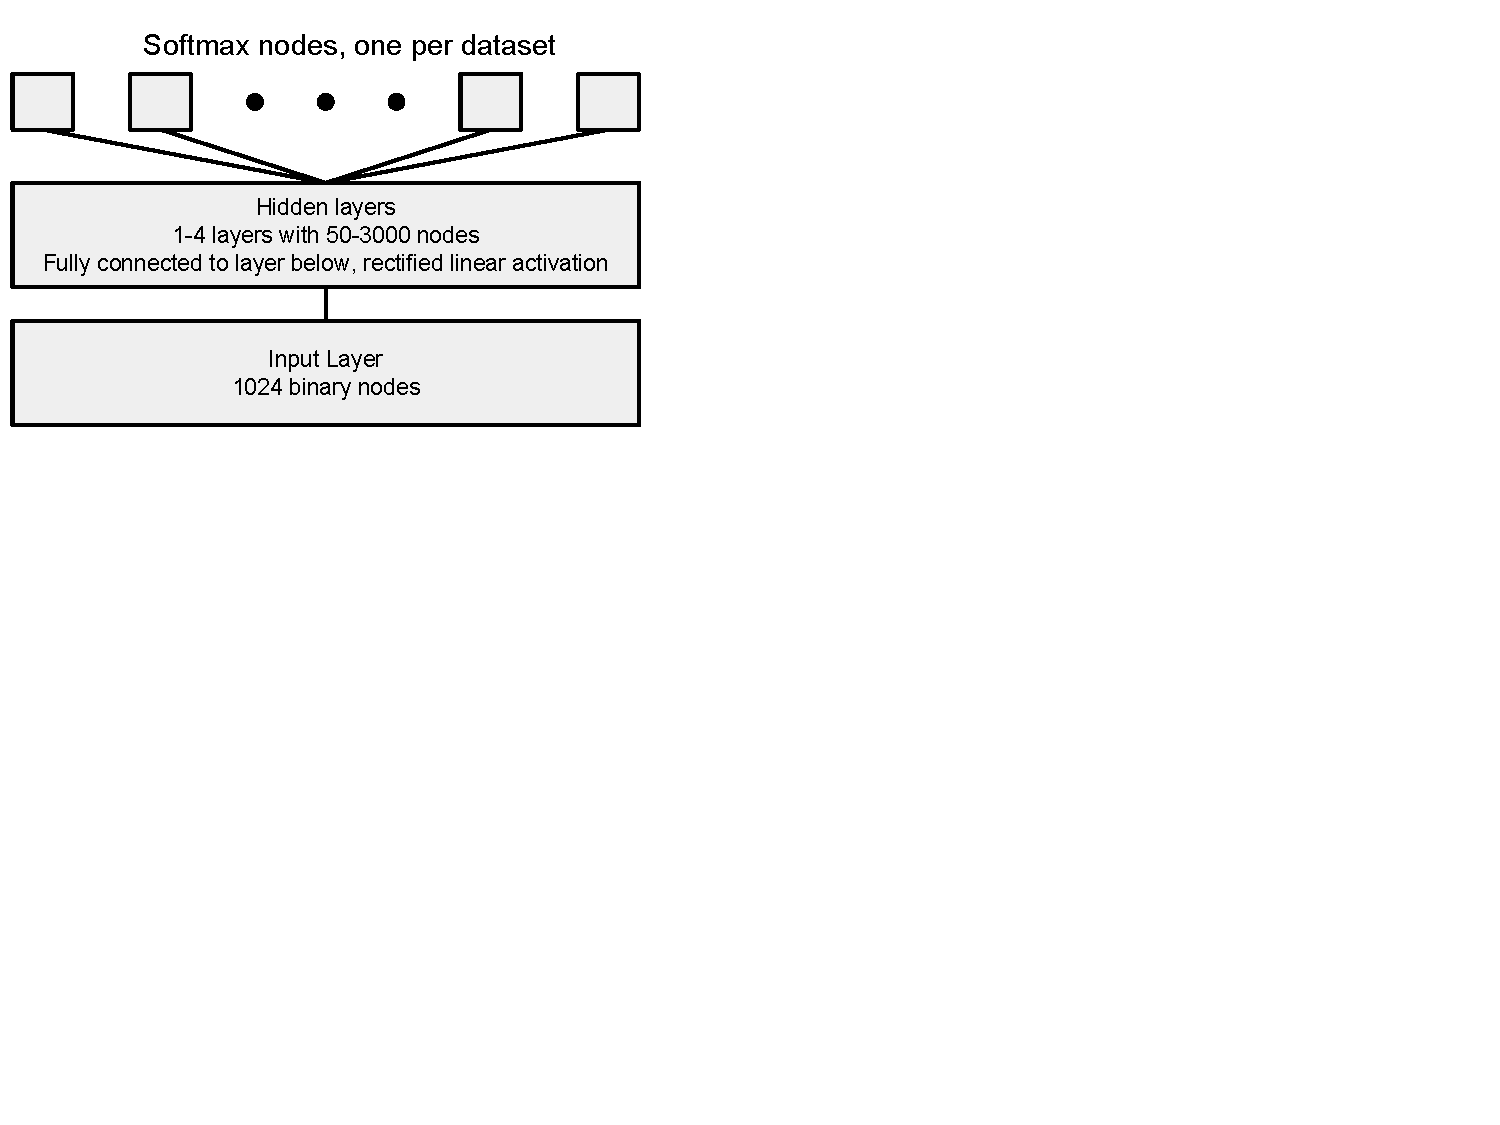
\includegraphics[trim=0 4.5in 5.5in 0,clip,width=0.9\linewidth]{Images/network.pdf}
\caption{Multitask neural network.}
\label{fig:network}
\end{figure}

\subsection{Experimental Section}

In this section, we seek to answer a number of questions about the
performance, capabilities, and limitations of massively multitask neural
networks:

\begin{enumerate}
\itemsep0em
\item Do massively multitask networks provide a performance boost over
  simple machine learning methods? If so, what is the optimal architecture
  for massively multitask networks?
\item How does the performance of a multitask network depend on the number
  of tasks? How does the performance depend on the total amount of data?
\item Do massively multitask networks extract generalizable information
  about chemical space?
\item When do datasets benefit from multitask training?
\end{enumerate}

The following subsections detail a series of experiments that seek to
answer these questions.

\subsubsection{Experimental Exploration of Massively Multitask Networks}
\label{sec:experimental}
We investigate the performance of multitask networks with various
hyperparameters and compare to several standard machine learning
approaches. Table~\ref{tab:exp_results} shows some of the highlights of our
experiments. Our best multitask architecture (pyramidal multitask networks)
significantly outperformed simpler models, including a hypothetical model
whose performance on each dataset matches that of the best single-task
model (Max\{LR, RF, STNN, PSTNN\}).

Every model we trained performed extremely well on the DUD-E datasets (all
models in Table~\ref{tab:exp_results} had median $5$-fold-average AUCs
$\ge0.99$), making comparisons between models on DUD-E uninformative. For
that reason, we exclude DUD-E from our subsequent statistical analysis.
However, we did not remove DUD-E from the training altogether because doing
so adversely affected performance on the other datasets (data not shown);
we theorize that DUD-E helped to regularize the classifier and avoid
overfitting.

\begin{table*}[t]
\small
\caption{Median $5$-fold-average AUCs for various models.  For each model,
  the sign test in the last column estimates the fraction of datasets
  (excluding the DUD-E group, for reasons discussed in the text) for which
  that model is superior to the PMTNN (bottom row). We use the Wilson score interval to
  derive a $95\%$ confidence interval for this fraction.  Non-neural
  network methods were trained using scikit-learn
  \cite{pedregosa2011scikit} implementations and a fixed set of hyperparameters.
  We also include results for a hypothetical ``best''
  single-task model (Max\{LR, RF, STNN, PSTNN\}) to provide a stronger
  baseline. Details for our cross-validation and training procedures are
  given in the Appendix.}
\label{tab:exp_results}
\vskip 0.2 in
\centering
\begin{tabular}{lcccc}
\toprule
Model & \makecell{PCBA \\ $(n=128)$} & \makecell{MUV \\ $(n=17)$} &
\makecell{Tox21 \\ $(n=12)$} & \makecell{Sign Test \\ CI} \\
\midrule
Logistic Regression (LR)& $.801$  & $.752$ & $.738$ & $[.04, .13]$ \\
Random Forest (RF) & $.800$  & $.774$  & $.790$ & $[.06, .16]$ \\
Single-Task Neural Net (STNN) & $.795$ & $.732$ & $.714$ & $[.04, .12]$ \\
Pyramidal $(2000, 100)$ STNN (PSTNN) & .809 & .745 & .740 & $[.06, .16]$ \\
Max\{LR, RF, STNN, PSTNN\} & $.824$ & $.781$ & $.790$ & $[.12, .24]$ \\
$1$-Hidden $(1200)$ Layer Multitask Neural Net (MTNN) & $.842$ & $.797$ & $.785$ & $[.08, .18]$ \\
Pyramidal $(2000, 100)$ Multitask Neural Net (PMTNN) & $\mathbf{.873}$ &
$\mathbf{.841}$ & $\mathbf{.818}$ & \\
\bottomrule
\end{tabular}
\end{table*}

During our first explorations, we had consistent problems with the networks
overfitting the data. As discussed in Section~\ref{sec:datasets}, our
datasets had a very small fraction of positive examples. For the single
hidden layer multitask network in Table~\ref{tab:exp_results}, each dataset
had $1200$ associated parameters. With a total number of positives in the
tens or hundreds, overfitting this number of parameters is a major issue in
the absence of strong regularization.

Reducing the number of parameters specific to each dataset is the
motivation for the pyramidal architecture. In our pyramidal networks, the
first hidden layer is very wide ($2000$ nodes) with a second narrow hidden
layer ($100$ nodes). This dimensionality reduction is similar in motivation
and implementation to the $1$x$1$ convolutions in the GoogLeNet
architecture~\cite{szegedy2014going}. The wide lower layer allows for
complex, expressive features to be learned while the narrow layer limits
the parameters specific to each task. Adding dropout of $0.25$ to our
pyramidal networks improved performance. We also trained single-task
versions of our best pyramidal network to understand whether this design
pattern works well with less data. Table~\ref{tab:exp_results} indicates
that these models outperform vanilla single-task networks but do not
substitute for multitask training.  Results for a variety of alternate
models are presented in the Appendix.

We investigated the sensitivity of our results to the sizes of the
pyramidal layers by running networks with all combinations of hidden layer
sizes: $(1000, 2000, 3000)$ and $(50, 100, 150)$.  Across the
architectures, means and medians shifted by $\le.01$~AUC with only MUV
showing larger changes with a range of $.038$.  We note that performance is
sensitive to the choice of learning rate and the number of training steps.
See the Appendix for details and data.

\subsubsection{Relationship between performance and number of tasks}
\label{sec:growth_curve}

The previous section demonstrated that massively multitask networks improve
performance over single-task models. In this section, we seek to understand
how multitask performance is affected by increasing the number of tasks.
\emph{A priori}, there are three reasonable ``growth curves'' (visually
represented in Figure~\ref{fig:growth_held_in}):
\begin{description}
\itemsep0em
\item[Over the hill:] performance initially improves, hits a maximum, then falls.
\item[Plateau:] performance initially improves, then plateaus.
\item[Still climbing:] performance improves throughout, but with a diminishing rate of
return.
\end{description}

\begin{figure}[ht]
\vskip 0.2in
\begin{center}
\centerline{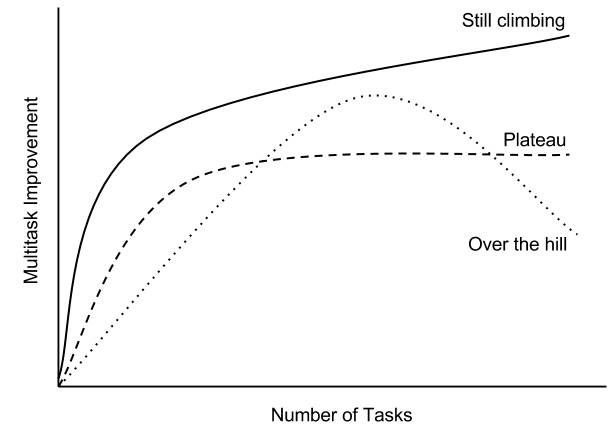
\includegraphics[width=0.7\linewidth]{Images/curves.png}}
\caption{Potential multitask growth curves}
\label{fig:growth_held_in}
\end{center}
\vskip -0.2in
\end{figure}

We constructed and trained a series of multitask networks on datasets
containing $10, 20, 40, 80, 160,$ and $249$ tasks. These datasets all
contain a fixed set of ten ``held-in'' tasks, which consists of a randomly
sampled collection of five PCBA, three MUV, and two Tox21 datasets.  These
datasets correspond to unique targets that do not have any obvious analogs
in the remaining collection. (We also excluded a similarly chosen set of
ten ``held-out'' tasks for use in Section~\ref{sec:embedding}). Each
training collection is a superset of the preceding collection, with tasks
added randomly. For each network in the series, we computed the mean
$5$-fold-average-AUC for the tasks in the held-in collection. We repeated
this experiment ten times with different choices of random seed.

\begin{figure}[ht]
\centering
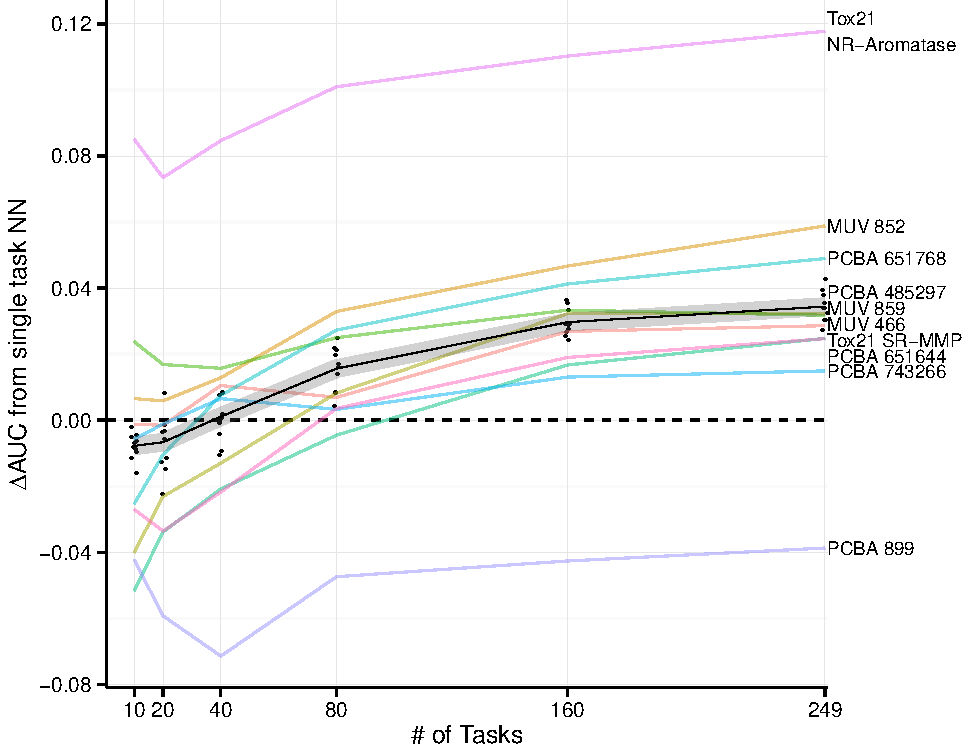
\includegraphics[width=\linewidth]{Images/held_in.pdf}
\caption{Held-in growth curves. The $y$-axis shows the change in AUC
  compared to a single-task neural network with the same architecture
  (PSTNN).  Each colored curve is the multitask improvement for a given
  held-in dataset. Black dots represent means across the $10$ held-in
  datasets for each experimental run, where additional tasks were randomly
  selected.  The shaded curve is the mean across the $100$ combinations of
  datasets and experimental runs.}
\label{fig:held-in}
\end{figure}

Figure~\ref{fig:held-in} plots the results of our experiments. The shaded
region emphasizes the average growth curve, while black dots indicate
average results for different experimental runs. The figure also displays
lines associated with each held-in dataset. Note that several datasets show
initial dips in performance. However, all datasets show subsequent
improvement, and all but one achieves performance superior to the
single-task baseline. Within the limits of our current dataset collection,
the distribution in \figurename~\ref{fig:held-in} agrees with either
plateau or still climbing. The mean performance on the held-in set is still
increasing at $249$ tasks, so we hypothesize that performance is
\textbf{still climbing}. It is possible that our collection is too small
and that an alternate pattern may eventually emerge.

\subsubsection{More tasks or more data?}

In the previous section we studied the effects of adding more tasks, but
here we investigate the relative importance of the total amount of data vs.
the total number of tasks. Namely, is it better to have many tasks with a
small amount of associated data, or a small number of tasks with a large
amount of associated data?

We constructed a series of multitask networks with $10, 15, 20, 30, 50$ and
$82$ tasks. As in the previous section, the tasks are randomly associated
with the networks in a cumulative manner (\emph{i.e.}, the $82$-task
network contained all tasks present in the $50$-task network, and so on).
All networks contained the ten held-in tasks described in the previous
section. The $82$ tasks chosen were associated with the largest datasets in
our collection, each containing $300$K-$500$K data points. Note that all of
these tasks belonged to the PCBA group.

We then trained this series of networks multiple times with $1.6$M, $3.3$M,
$6.5$M, $13$M, and $23$M data points sampled from the non-held-in tasks. We
perform the sampling such that for a given task, all data points present in
the first stage ($1.6$M) appeared in the second ($3.3$M), all data points
present in the second stage appeared in the third ($6.5$M), and so on. We
decided to use larger datasets so we could sample meaningfully across this
entire range. Some combinations of tasks and data points were not realized;
for instance, we did not have enough data to train a $20$-task network with
$23$M additional data points. We repeated this experiment ten times using
different random seeds.

\figurename~\ref{fig:data_tasks} shows the results of our experiments. The
$x$-axis tracks the number of additional tasks, while the $y$-axis displays
the improvement in performance for the held-in set relative to a multitask
network trained only on the held-in data. When the total amount of data is
fixed, having more tasks consistently yields improvement. Similarly, when
the number of tasks is fixed, adding additional data consistently improves
performance. Our results suggest that the total amount of data and the
total number of tasks both contribute significantly to the multitask
effect.

\begin{figure}[ht]
\centering
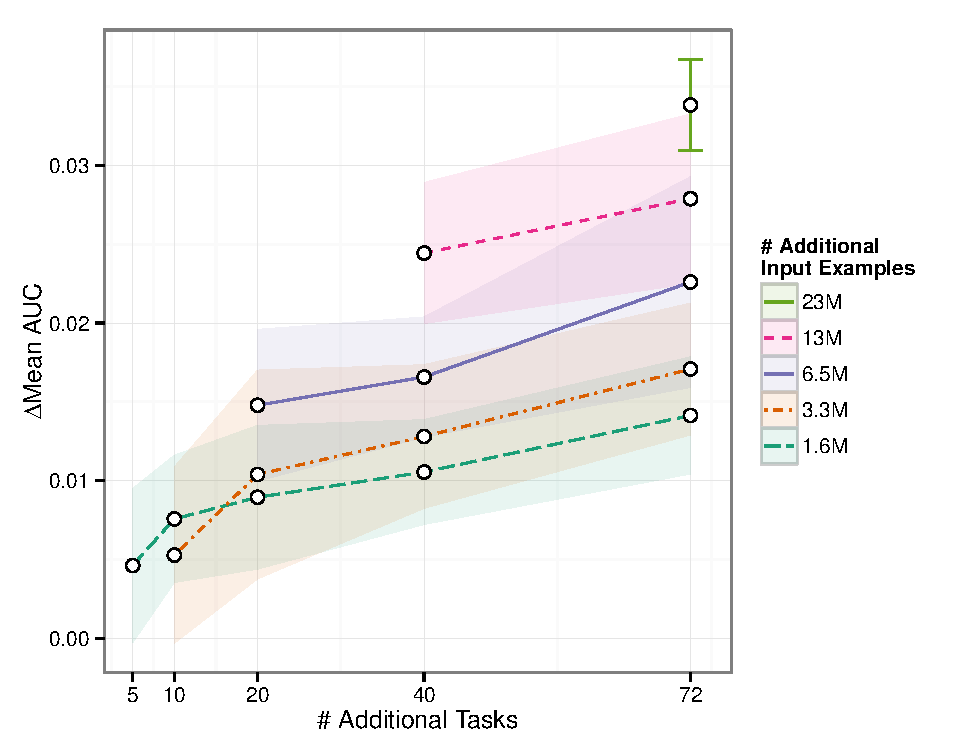
\includegraphics[width=\linewidth]{Images/grid_final.pdf}
\caption{Multitask benefit from increasing tasks and data independently.
  As in \figurename~\ref{fig:growth_held_in}, we added randomly selected
  tasks ($x$-axis) to a fixed held-in set. A stratified random sampling
  scheme was applied to the additional tasks in order to achieve fixed
  total numbers of additional input examples (color, line type).  White
  points indicate the mean over $10$ experimental runs of $\Delta$ mean-AUC
  over the initial network trained on the $10$ held-in datasets. Color-filled
  areas and error bars describe the smoothed $95\%$ confidence intervals.}
\label{fig:data_tasks}
\end{figure}

\subsubsection{Do massively multitask networks extract generalizable features?}
\label{sec:embedding}

The features extracted by the top layer of the network represent
information useful to many tasks. Consequently, we sought to determine the
transferability of these features to tasks not in the training set.  We
held out ten data sets from the growth curves calculated in
Section~\ref{sec:growth_curve} and used the learned weights from points
along the growth curves to initialize single-task networks for the held-out
datasets, which we then fine-tuned.

The results of training these networks (with $5$-fold stratified
cross-validation) are shown in \figurename~\ref{fig:held_out}. First, note
that many of the datasets performed worse than the baseline when
initialized from the 10-held-in-task networks. Further, some datasets never
exhibited any positive effect due to multitask initialization. Transfer
learning can be negative.

Second, note that the transfer learning effect became stronger as multitask
networks were trained on more data. Large multitask networks exhibited
better transferability, but the average effect even with $249$ datasets was
only $\sim.01$ AUC.  We hypothesize that the extent of this
generalizability is determined by the presence or absence of relevant data
in the multitask training set.

\begin{figure}[ht]
\vskip 0.2in
\begin{center}
\centerline{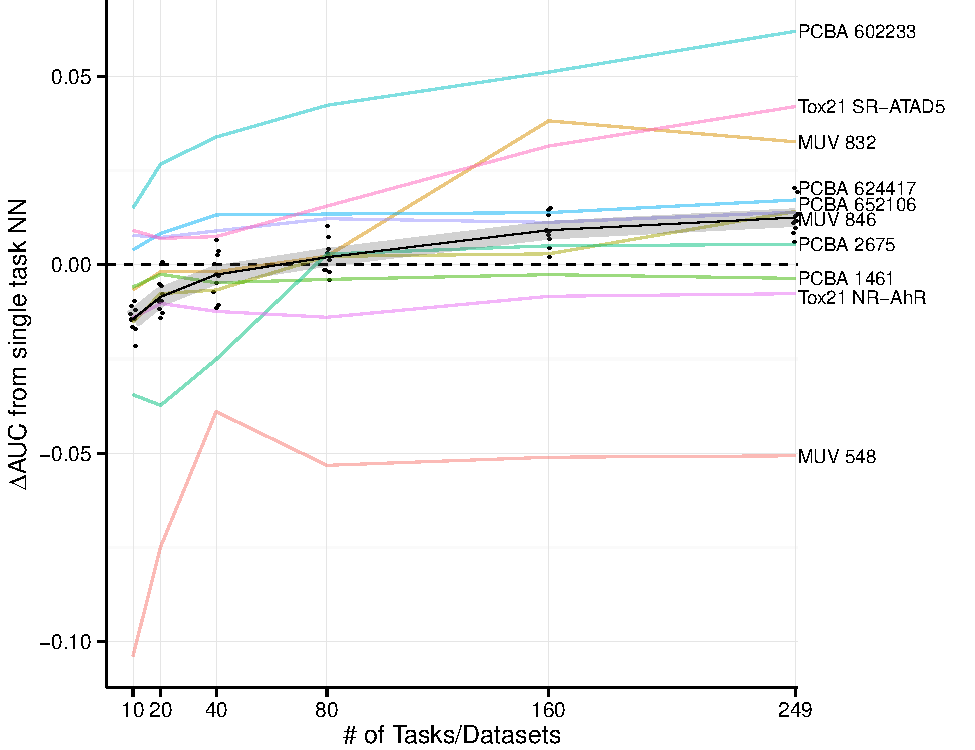
\includegraphics[width=\linewidth]{Images/held_out_v2.pdf}}
\caption{Held-out growth curves. The $y$-axis shows the change in AUC
  compared to a single-task neural network with the same architecture
  (PSTNN). Each colored curve is the result of initializing a single-task
  neural network from the weights of the networks from
  Section~\ref{sec:growth_curve} and computing the mean across the $10$
  experimental runs. These datasets were \emph{not} included in the
  training of the original networks. The shaded curve is the mean across
  the $100$ combinations of datasets and experimental runs, and black dots
  represent means across the $10$ held-out datasets for each experimental
  run, where additional tasks were randomly selected.}
\label{fig:held_out}
\end{center}
\vskip -0.2in
\end{figure}

\subsubsection{When do Datasets Benefit from Multitask Training?}

The results in Sections \ref{sec:growth_curve} and \ref{sec:embedding}
indicate that some datasets benefit more from multitask training than
others. In an effort to explain these differences, we consider three
specific questions:
\begin{enumerate}
\itemsep0em
\item Do some biological target classes realize greater multitask
  improvement than others?
\item Do tasks associated with duplicated targets have artificially high
  multitask performance?
\item Do shared active compounds explain multitask improvement?
\end{enumerate}

\paragraph{Target Classes}

\figurename~\ref{fig:target_similarity} shows the relationship between
multitask improvement and target classes. As before, we report multitask
improvement in terms of $\Delta$ mean-AUC and exclude the DUD-E datasets.
Nearly every target class realized gains, suggesting that the
multitask framework is applicable to experimental data from multiple target
classes.

\begin{figure}[ht]
\centering
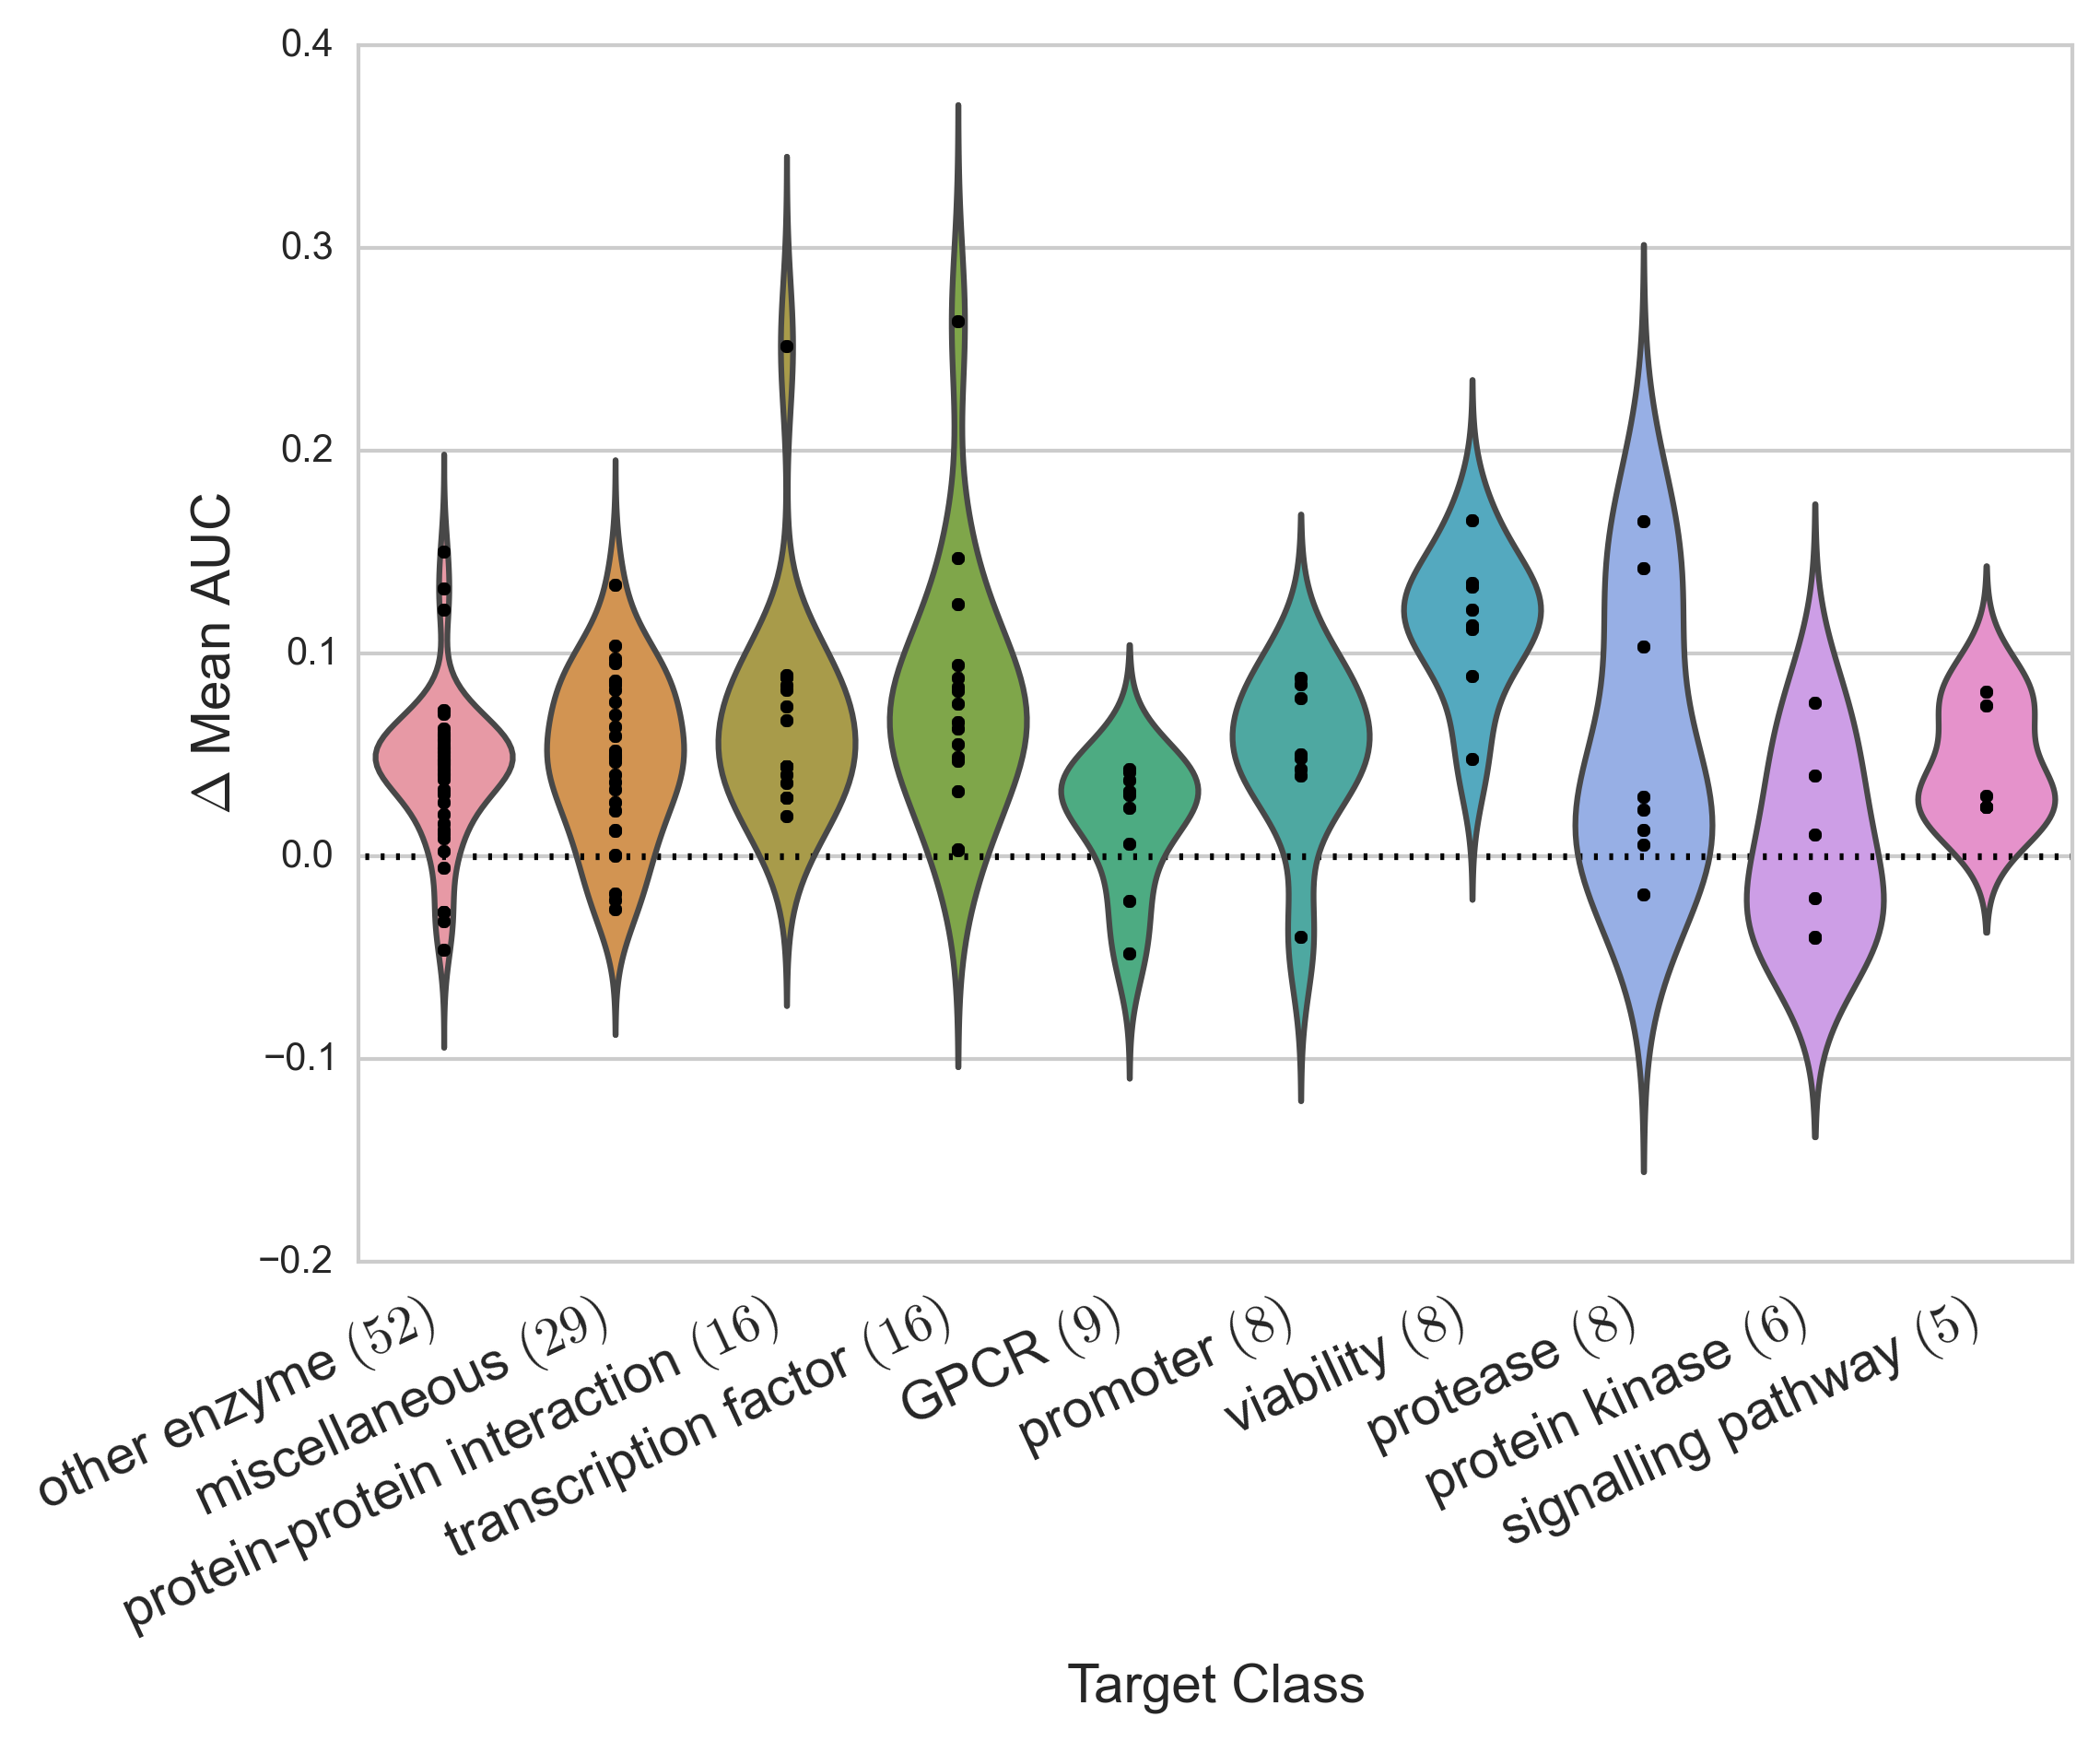
\includegraphics[width=0.9\linewidth]{Images/target_classes.png}
\caption{Multitask improvement across target classes. The $x$-coordinate
  lists a series of biological target classes represented in our dataset
  collection, and the $y$-coordinate is the difference in mean-AUC
  between multitask and single-task models. Note that the DUD-E datasets
  are excluded. Classes are ordered by total number of targets (in
  parenthesis), and target classes with fewer than five members are merged
  into ``miscellaneous.''}
\label{fig:target_similarity}
\end{figure}

\paragraph{Duplicate Targets}
\label{sec:duplicates}

As mentioned in Section~\ref{sec:datasets}, there are many cases of tasks
with identical targets. We compared the multitask improvement of duplicate
vs. unique tasks. The distributions have substantial overlap (see the
Appendix), but the average improvement was slightly higher for
duplicated tasks ($0.059$ vs. $0.032$; a one-sided $t$-test between the
duplicate and unique distributions gave $p=0.161$). Sign
tests for single-task vs. multitask models for duplicate and unique
targets gave significant and highly overlapping confidence intervals
($[0.11, 0.36]$ and $[0.11, 0.24]$, respectively; recall that the meaning
of these intervals is given in the caption for
\tablename~\ref{tab:exp_results}). Together, these results suggest that
there is not significant information leakage within multitask networks.
Consequently, the results of our analysis are unlikely to be significantly
affected by the presence of duplicate targets in our dataset collection.

\paragraph{Shared Active Compounds}
\label{sec:similarity}

The biological context of our datasets implies that active compounds
contain more information than inactive compounds; while an inactive
compound may be inactive for many reasons, active compounds often rely on
similar physical mechanisms. Hence, shared active compounds should be a
good measure of dataset similarity.

We compared multitask improvement against a measure of dataset similarity we
call ``active occurrence rate'' (AOR), based on the number of active compounds
shared between datasets (see Appendix for details). Surprisingly, there does
not appear to be any significant correlation between AOR and $\Delta$
mean-AUC ($r^2=0.09$). Further work is needed to identify factors that
contribute to multitask improvement.

\subsection{Discussion and Conclusion}
In this work, we investigated the use of massively multitask networks for
virtual screening. We gathered a large collection of publicly available
experimental data that we used to train massively multitask neural
networks. These networks achieved significant improvement over simple
machine learning algorithms.

We explored several aspects of the multitask framework. First, we
demonstrated that multitask performance improved with the addition of more
tasks; our performance was still climbing at 259 tasks. Next, we considered
the relative importance of introducing more data vs. more tasks. We found
that additional data and additional tasks both contributed significantly to
the multitask effect. We next discovered that multitask learning afforded
limited transferability to tasks not contained in the training set. This
effect was not universal, and required large amounts of data even when it
did apply.

We observed that the multitask effect was stronger for some datasets than
others. Consequently, we investigated possible explanations for this
discrepancy and found that the presence of shared active compounds was
moderately correlated with multitask improvement, but the biological class
of the target was not. It is also possible that multitask improvement
results from accurately modeling experimental artifacts rather than
specific interactions between targets and small molecules. We do not
believe this to be the case, as we demonstrated strong improvement on the
thoroughly-cleaned MUV datasets.

The efficacy of multitask learning is directly related to the availability
of relevant data. Hence, obtaining greater amounts of data is of critical
importance for improving the state of the art. Major pharmaceutical
companies possess vast private stores of experimental measurements; our
work provides a strong argument that increased data sharing could result in
benefits for all.

More data will maximize the benefits achievable using current
architectures, but in order for algorithmic progress to occur, it must be
possible to judge the performance of proposed models against previous work.
It is disappointing to note that all published applications of deep
learning to virtual screening (that we are aware of) use distinct datasets
that are not directly comparable. It remains to future research to
establish standard datasets and performance metrics for this field.

Another direction for future work is the further study of small molecule
featurization. In this work, we use only one possible featurization
(ECFP4), but there exist many others. Additional performance may also be
realized by considering targets as well as small molecules in the
featurization. Yet another line of research could improve performance by
using unsupervised learning to explore much larger segments of chemical
space.

Although deep learning offers interesting possibilities for virtual
screening, the full drug discovery process remains immensely complicated.
Can deep learning---coupled with large amounts of experimental
data---trigger a revolution in this field? Considering the transformational
effect that these methods have had on other fields, we are optimistic about
the future.

\subsection*{Acknowledgments} B.R. was supported by the Fannie and John Hertz
Foundation. S.K. was supported by a Smith Stanford Graduate Fellowship.
We also acknowledge support from NIH and NSF, in particular NIH U54
GM072970 and NSF 0960306. The latter award was funded under the American
Recovery and Reinvestment Act of 2009 (Public Law 111-5).

%\bibliography{icml2015}
%\bibliographystyle{abbrv}
%\end{document}
%\clearpage
%\section{MoleculeNet: A Benchmark for Molecular Machine Learning}

\subsection{Abstract}
Molecular machine learning has been maturing rapidly over the last few years. Improved methods and the presence of larger datasets have enabled machine learning algorithms to make increasingly accurate predictions about molecular properties. However, algorithmic progress has been limited due to the lack of a standard benchmark to compare the efficacy of proposed methods; most new algorithms are benchmarked on different datasets making it challenging to gauge the quality of proposed methods. This work introduces MoleculeNet, a large scale benchmark for molecular machine learning. MoleculeNet curates multiple public datasets, establishes metrics for evaluation, and offers high quality open-source implementations of multiple previously proposed molecular featurization and learning algorithms (released as part of the DeepChem open source library). MoleculeNet benchmarks demonstrate that learnable representations are powerful tools for molecular machine learning and broadly offer the best performance. However, this result comes with caveats. Learnable representations still struggle to deal with complex tasks under data scarcity and highly imbalanced classification. For quantum mechanical and biophysical datasets, the use of physics-aware featurizations can be more important than choice of particular learning algorithm. \\%The abstrast goes here instead of the text "The abstract should be..."

%\end{tabular}

%\end{@twocolumnfalse} \vspace{0.6cm}

%]
%%%END OF TITLE, AUTHORS AND ABSTRACT%%%

%%%FONT SETUP - please do not change any commands within this section
%\renewcommand*\rmdefault{bch}\normalfont\upshape
%\rmfamily
%\section*{}
%\vspace{-1cm}


%%%FOOTNOTES%%%

%\footnotetext{\textit{$^{a}$~Department of Chemistry, Stanford %University, Stanford, CA 94305, USA. E-mail: pande@stanford.edu}}
%\footnotetext{\textit{$^{b}$~Department of Computer Science, Stanford University, Stanford, CA 94305, USA}}
%\footnotetext{\textit{$^{c}$~Program in Biophysics, Stanford School of Medicine, Stanford, CA 94305, USA}}
%\footnotetext{\textit{$^{d}$~Schrodinger Inc., USA}}



%Please use \dag to cite the ESI in the main text of the article.
%If you article does not have ESI please remove the the \dag symbol from the title and the footnotetext below.
%\footnotetext{\dag~Electronic Supplementary Information (ESI) available: [details of any supplementary information available should be included here]. See DOI: 10.1039/b000000x/}
%additional addresses can be cited as above using the lower-case letters, c, d, e... If all authors are from the same address, no letter is required

%\footnotetext{\ddag~Joint First Authorship}
%\footnotetext{\P~Joint Second Authorship}


%%%END OF FOOTNOTES%%%


%%%MAIN TEXT%%%%
\subsection{Introduction} \label{Introduction}

Overlap between chemistry and 
statistical learning has had a long history. The field of cheminformatics has been utilizing machine learning methods in chemical modeling(e.g. quantitative structure activity relationships, QSAR) for decades.\cite{gasteiger1993neural, zupan1999neural, varnek2012machine, mitchell2014machine,devillers1996neural, schneider1998artificial} In the recent 10 years, with the advent of sophisticated deep learning methods \cite{DeepLearning, schmidhuber2015deep}, machine learning has gathered increasing amounts of attention from the scientific community. Data-driven analysis has become a routine step in many chemical and biological applications, including virtual screening\cite{ma2015deep, ramsundar2015massively, unterthiner2014deep, AtomNet}, chemical property prediction\cite{ESOL_dataset, lusci2013deep, SAMPL4, FreeSolv}, and quantum chemistry calculations\cite{GDB7_dataset_prl, GDB7_dataset_arxiv, schutt2016quantum, mcgibbon2017improving}. 

In many such applications, machine learning has shown strong potential to compete with or even outperform conventional \textit{ab-initio} computations\cite{FreeSolv, GDB7_dataset_arxiv}. It follows that introduction of novel machine learning methods has the potential to reshape research on properties of molecules. However, this potential has been limited by the lack of a standard evaluation platform for proposed machine learning algorithms. Algorithmic papers often benchmark proposed methods on disjoint dataset collections, making it a challenge to gauge whether a proposed technique does in fact improve performance.

Data for molecule-based machine learning tasks are highly heterogeneous and expensive to gather. Obtaining precise and accurate results for chemical properties typically requires specialized instruments as well as expert supervision (contrast with computer speech and vision, where lightly trained workers can annotate data suitable for machine learning systems). As a result, molecular datasets are usually much smaller than those available for other machine learning tasks. Furthermore, the breadth of chemical research means our interests with respect to a molecule may range from quantum characteristics to measured impacts on the human body. Molecular machine learning methods have to be capable of learning to predict this very broad range of properties. Complicating this challenge, input molecules can have arbitrary size and components, highly variable connectivity and many three dimensional conformers (three dimensional molecular shapes). To transform molecules into a form suitable for conventional machine learning algorithms (that usually accept fixed length input), we have to extract useful and related information from a molecule into a fixed dimensional representation (a process called featurization).\cite{ECFP, graphconv_feat, kearnes2016graphconv}.  

To put it simply, building machine learning models on molecules requires overcoming several key issues: limited amounts of data, wide ranges of outputs to predict, large heterogeneity in input molecular structures and appropriate learning algorithms. Therefore, this work aims to facilitate the development of molecular machine learning methods by curating a number of dataset collections, creating a suite of software that implements many known featurizations of molecules, and providing high quality implementations of many previously proposed algorithms. Following the footsteps of WordNet\cite{wordnet} and ImageNet\cite{imagenet_cvpr09}, we call our suite MoleculeNet, a benchmark collection for molecular machine learning.

In machine learning, a benchmark serves as more than a simple collection of data and methods. The introduction of the ImageNet benchmark in 2009 has triggered a series of breakthroughs in computer vision, and in particular has facilitated the rapid development of deep convolutional networks. The ILSVRC, an annual contest held by the ImageNet team\cite{ILSVRC15}, draws considerable attention from the community, and greatly stimulates collaborations and competitions across the field. The contest has given rise to a series of prominent machine learning models such as AlexNet\cite{alexnet}, GoogLeNet\cite{googlenet}, ResNet\cite{resnet} which have had broad impact on the academic and industrial computer science communities. We hope that MoleculeNet will trigger similar breakthroughs by serving as a platform for the wider community to develop and improve models for learning molecular properties.

In particular, MoleculeNet contains data on the properties of over 700,000 compounds. All datasets have been curated and integrated into the open source DeepChem package.\cite{deepchem} Users of DeepChem can easily load all MoleculeNet benchmark data through provided library calls. MoleculeNet also contributes high quality implementations of well known (bio)chemical featurization methods. To facilitate comparison and development of new methods, we also provide high quality implementations of several previously proposed machine learning methods. Our implementations are integrated with DeepChem, and depend on Scikit-Learn \cite{pedregosa2011scikit} and Tensorflow \cite{abadi2016tensorflow} underneath the hood. Finally, evaluation of machine learning algorithms requires defined methods to split datasets into training/validation/test collections. Random splitting, common in machine learning, is often not correct for chemical data \cite{sheridan2013time}. MoleculeNet contributes a library of splitting mechanisms to DeepChem and evaluates all algorithms with multiple choices of data split. MoleculeNet provide a series of benchmark results of implemented machine learning algorithms using various featurizations and splits upon our dataset collections. These results are provided within this paper, and will be maintained online in an ongoing fashion as part of DeepChem. 

The related work section will review prior work in the chemistry community on gathering curated datasets and discuss how MoleculeNet differs from these previous efforts. The methods section reviews the dataset collections, metrics, featurization methods, and machine learning models included as part of MoleculeNet. The results section will analyze the benchmarking results to draw conclusions about the algorithms and datasets considered.

\subsection{Related Work}
MoleculeNet draws upon a broader movement within the chemical community to gather large sources of curated data. PubChem \cite{bolton2008pubchem} and PubChem BioAssasy \cite{pcba_dataset} gather together thousands of bioassay results, along with millions of unique molecules tested within these assays. The ChEMBL database offers a similar service, with millions of bioactivity outcomes across thousands of protein targets. Both PubChem and ChEMBL are human researcher oriented, with web portals that facilitate browsing of the available targets and compounds. ChemSpider is a repository of nearly 60 million chemical structures, with web based search capabilities for users. The Crystallography Open Database \cite{gravzulis2009crystallography} and Cambridge Structural Database \cite{groom2016cambridge} offer large repositories of organic and inorganic compounds. The protein data bank \cite{berman2003announcing} offers a repository of experimentally resolved three dimensional protein structures. This listing is by no means comprehensive; the methods subsection will discuss a number of smaller data sources in greater detail.

These past efforts have been critical in enabling the growth of computational chemistry. However, these previous databases are not machine-learning focused. In particular, these collections don't define metrics which measure the effectiveness of algorithmic methods in understanding the data contained. Furthermore, there is no prescribed separation of the data into training/validation/test sets (critical for machine learning development). Without specified metrics or splits, the choice is left to individual researchers, and there are indeed many chemical machine learning papers which use subsets of these data stores for machine learning evaluation. Unfortunately, the choice of metric and subset varies widely between groups, so two methods papers using PubChem data may be entirely incomparable. MoleculeNet aims to bridge this gap by providing benchmark results for a reasonable range of metrics, splits, and subsets of these (and other) data collections.

It's important to note that there have been some efforts to create benchmarking datasets for machine learning in chemistry. The Quantum Machine group \cite{QuantumMachine} and previous work on multitask learning \cite{ramsundar2015massively} both introduce benchmarking collections which have been used in multiple papers. MoleculeNet incorporates data from both these efforts and significantly expands upon them.

\subsection{Methods}

\begin{figure*}
  \centering
  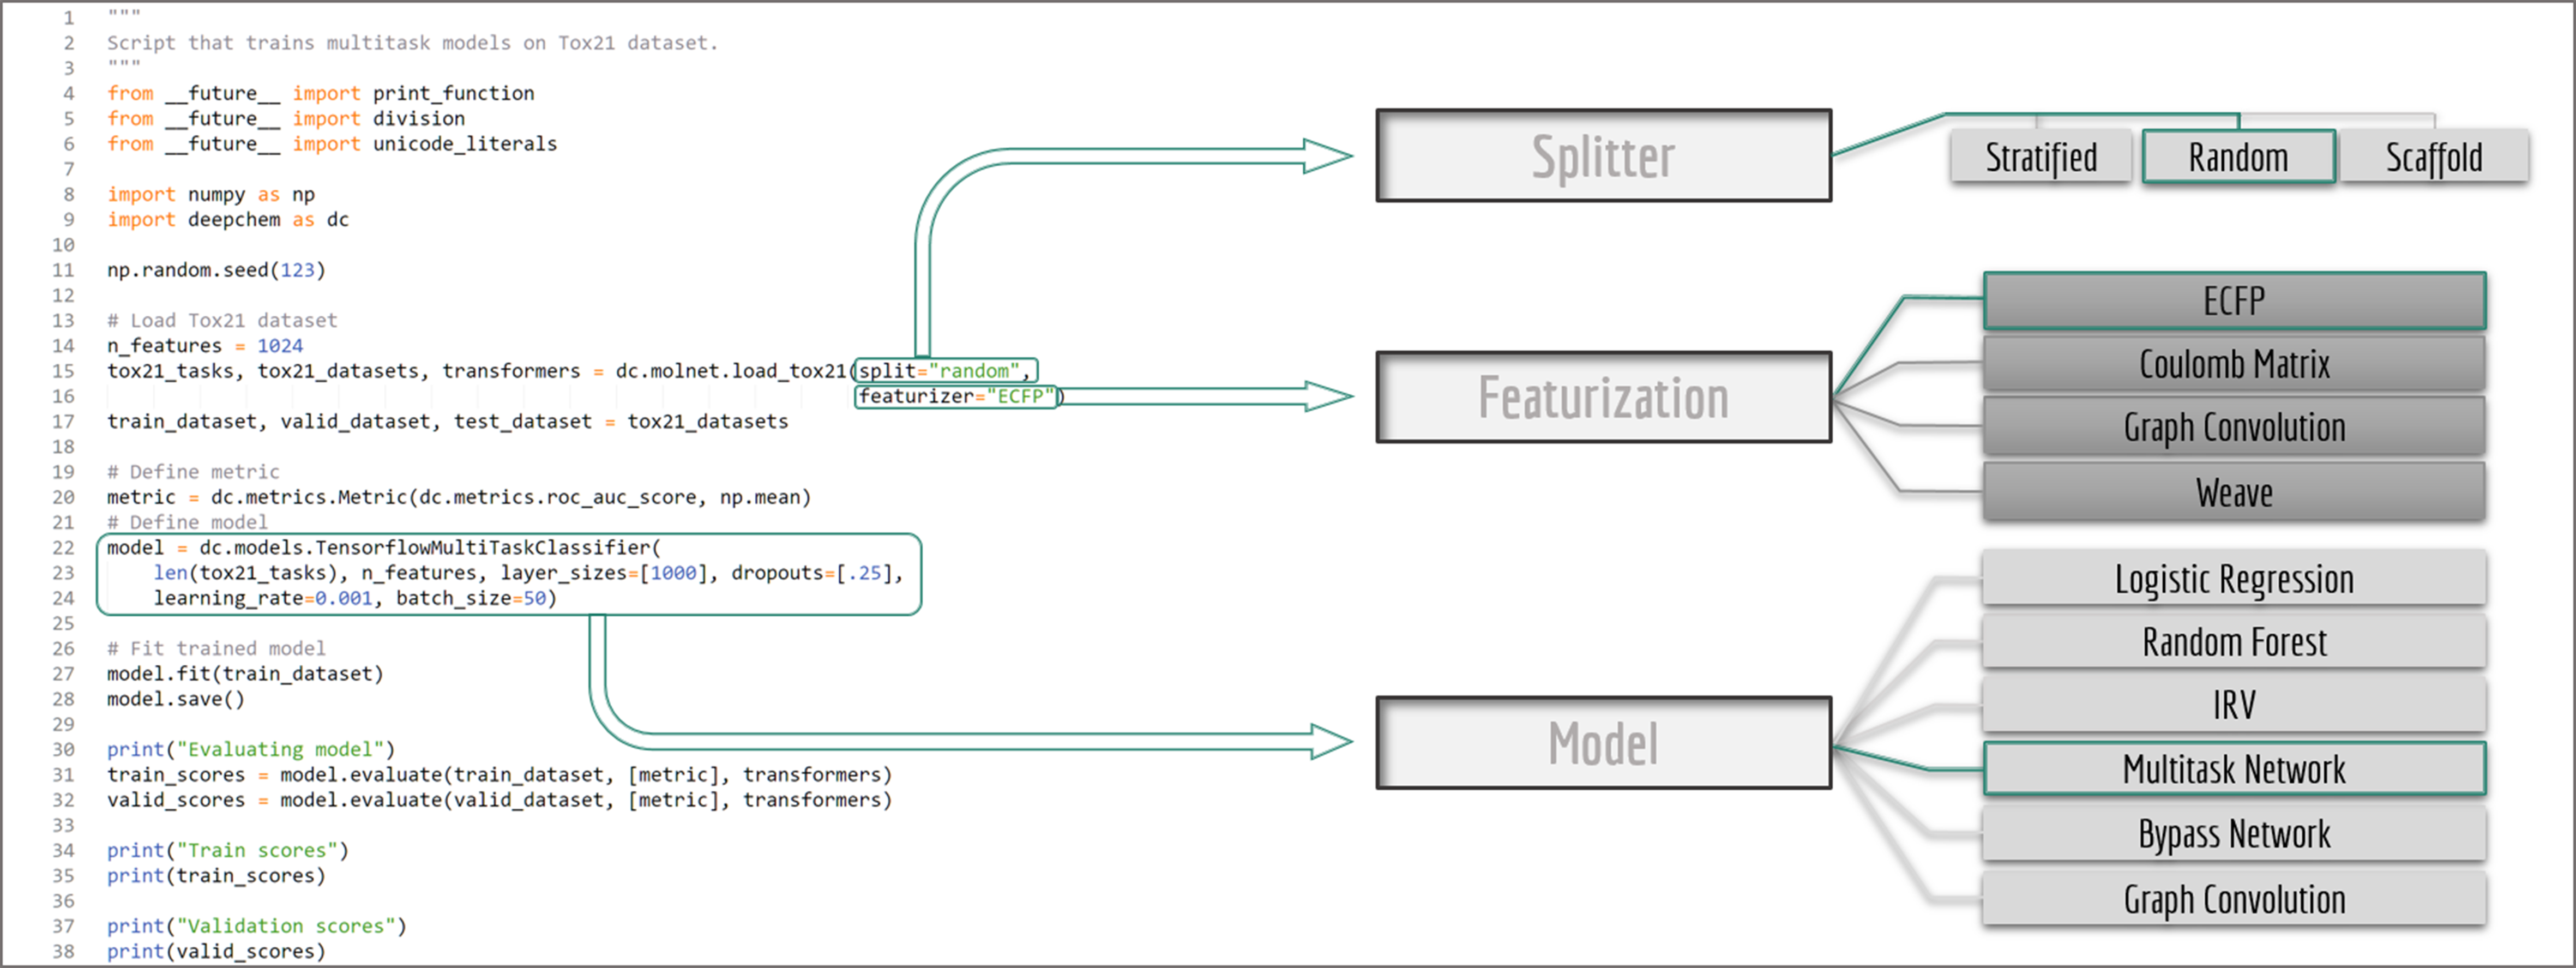
\includegraphics[width=0.9\textwidth]{Images/benchmark_framework.png}
  \caption{Example code for benchmark evaluation with DeepChem, multiple methods are provided for data splitting, featurization and learning.}
  \label{fig:benchmark_example}
\end{figure*}

MoleculeNet is based on the open source package DeepChem\cite{deepchem}. Figure~\ref{fig:benchmark_example} shows an annotated DeepChem benchmark script. Note how different choices for data splitting, featurization, and model are available. DeepChem also directly provides molnet sub-module to support benchmarking. The single line below runs benchmarking on the specified dataset, model and featurizer. User defined models capable of handling DeepChem datasets are also supported.

{\fontfamily{pcr}\selectfont
deepchem.molnet.run\_benchmark(datasets, model, split, featurizer)
}

In this section, we will further elaborate the benchmarking system, introducing available datasets as well as implemented splitting, metrics, featurization, and learning methods.


\subsubsection{Datasets}
MoleculeNet is built upon multiple public databases. The full collection currently includes over 700,000 compounds tested on a range of different properties. These properties can be subdivided into four categories: quantum mechanics, physical chemistry, biophysics and physiology. As illustrated in Figure~\ref{fig:dataset_composition}, separate datasets in the MoleculeNet collection cover various levels of molecular properties, ranging from molecular-level properties to macroscopic influences on human body. For each dataset, we propose a metric and a splitting pattern(introduced in the following texts) that best fit the properties of the dataset. Performances on the recommended metric and split are reported in the results section.

In most datasets, SMILES strings\cite{SMILES} are used to represent input molecules, 3D coordinates are also included in part of the collection as molecular features, which enables different methods to be applied. Properties, or output labels, are either 0/1 for classification tasks, or floating point numbers for regression tasks. At the time of writing, MoleculeNet contains 17 datasets prepared and benchmarked, but we anticipate adding further datasets in an on-going fashion. We also highly welcome contributions from other public data collections. For more detailed dataset structure requirements and instructions on curating datasets, please refer to the tutorial notebook in the example folder of DeepChem github repository.

Table~\ref{tab:n_samples} lists details of datasets in the collection, including tasks, compounds and their features, recommended splits and metrics. Contents of each dataset will be elaborated in this subsection, function calls to access the datasets can be found in the supplementary information\dag.

\begin{figure*}[h]
  \centering
  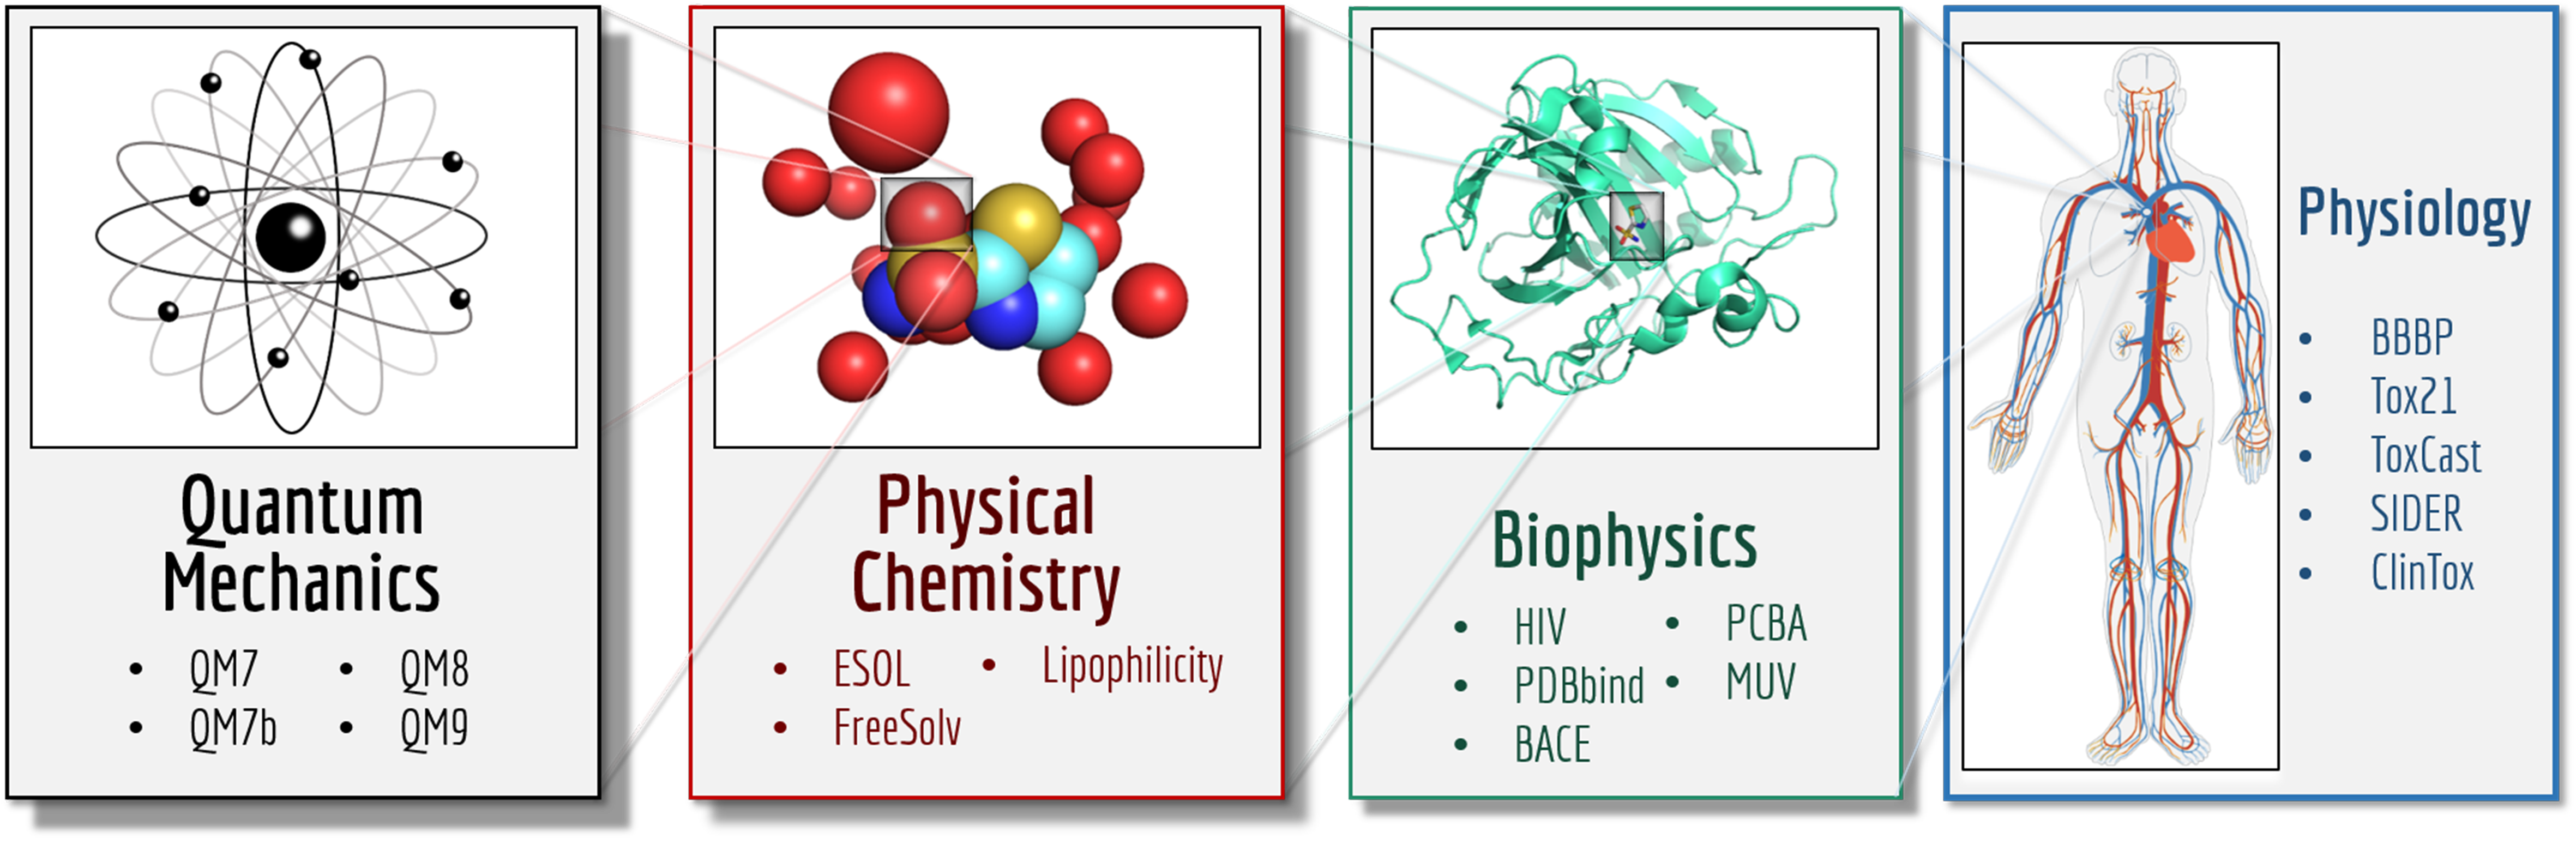
\includegraphics[width=.85\textwidth]{Images/dataset_composition.png}
  \caption{Tasks in different datasets focus on different levels of properties of molecules.}
  \label{fig:dataset_composition}
\end{figure*}

\paragraph{QM7/QM7b}

The QM7/QM7b datasets are subsets of the GDB-13 database\cite{GDB13}, a database of nearly 1 billion stable and synthetically accessible organic molecules, containing up to seven ``heavy'' atoms (C, N, O, S). The 3D Cartesian coordinates of the most stable conformation and electronic properties (atomization energy, HOMO/LUMO eigenvalues, etc.) of each molecule were determined using \textit{ab-initio} density functional theory (PBE0/tier2 basis set).\cite{GDB7_dataset_prl, GDB7_dataset_arxiv} Learning methods benchmarked on QM7/QM7b are responsible for predicting these electronic properties given stable conformational coordinates. For the purpose of more stable performances as well as better comparison, we recommend stratified splitting(introduced in the next subsection) for QM7.

\paragraph{QM8}

The QM8 dataset comes from a recent study on modeling quantum mechanical calculations of electronic spectra and excited state energy of small molecules.\cite{QM8} Multiple methods, including time-dependent density functional theories (TDDFT) and second-order approximate coupled-cluster (CC2), are applied to a collection of molecules that include up to eight heavy atoms (also a subset of the GDB-17 database\cite{GDB-17}). In total, four exicted state properties are calculated by three different methods on 22 thousand samples.

\paragraph{QM9}

QM9 is a comprehensive dataset that provides geometric, energetic, electronic and thermodynamic properties for a subset of GDB-17 database\cite{GDB-17}, comdprising 134 thousand stable organic molecules with up to nine heavy atoms\cite{QM9}. All moleucles are modeled using density functional theory (B3LYP/6-31G(2df,p) based DFT). In our benchmark, geometric properties (atomic coordinates) are integrated into features, which are then applied to predict other properties.

The datasets introduced above (QM7, QM7b, QM8, QM9) were curated as part of the Quantum-Machine effort \cite{QuantumMachine}, which has processed a number of datasets to measure the efficacy of machine-learning methods for quantum chemistry.

\paragraph{ESOL}

ESOL is a small dataset consisting of water solubility data for 1128 compounds.\cite{ESOL_dataset} The dataset has been used to train models that estimate solubility directly from chemical structures (as encoded in SMILES strings).\cite{graphconv_feat} Note that these structures don't include 3D coordinates, since solubility is a property of a molecule and not of its particular conformers.

\paragraph{FreeSolv}
The Free Solvation Database (FreeSolv) provides experimental and calculated hydration free energy of small molecules in water\cite{FreeSolv}. A subset of the compounds in the dataset are also used in the SAMPL blind prediction challenge\cite{SAMPL4}. The calculated values are derived from alchemical free energy calculations using molecular dynamics simulations. We include the experimental values in the benchmark collection, and use calculated values for comparison.

\paragraph{Lipophilicity}

Lipophilicity is an important feature of drug molecules that affects both membrane permeability and solubility. This dataset, curated from ChEMBL database,\cite{Hersey2015lipo} provides experimental results of octanol/water distribution coefficient (logD at pH 7.4) of 4200 compounds.

\paragraph{PCBA}

PubChem BioAssay (PCBA) is a database consisting of biological activities of small molecules generated by high-throughput screening.\cite{pcba_dataset} We use a subset of PCBA, containing 128 bioassays measured over 400 thousand compounds, used by previous work to benchmark machine learning methods.\cite{ramsundar2015massively}

\paragraph{MUV}

The Maximum Unbiased Validation (MUV) group is another benchmark dataset selected from PubChem BioAssay by applying a refined nearest neighbor analysis.\cite{muv_dataset} The MUV dataset contains 17 challenging tasks for around 90 thousand compounds and is specifically designed for validation of virtual screening techniques.

\paragraph{HIV}

The HIV dataset was introduced by the Drug Therapeutics Program (DTP) AIDS Antiviral Screen, which tested the ability to inhibit HIV replication for over 40,000 compounds.\cite{HIV} Screening results were evaluated and placed into three categories: confirmed inactive (CI), confirmed active (CA) and confirmed moderately active (CM). We further combine the latter two labels, making it a classification task between inactive (CI) and active (CA and CM). As we are more interested in discover new categories of HIV inhibitors, scaffold splitting(introduced in the next subsection) is recommended for this dataset.

\paragraph{PDBbind}

PDBbind is a comprehensive database of experimentally measured binding affinities for bio-molecular complexes.\cite{PDBbind1, PDBbind2} Unlike other ligand-based biological activity datasets, in which only the structures of ligands are provided, PDBbind provides detailed 3D Cartesian coordinates of both ligands and their target proteins derived from experimental (e.g., X-Ray crystallography) measurements. The availability of coordinates of the protein-ligand complexes permits structure-based featurization that is aware of the protein-ligand binding geometry. We use the ``refined'' and ``core'' subsets of the database\cite{PDBbind3}, more carefully processed for data artifacts, as additional benchmarking targets. Samples in PDBbind dataset are collected over a relatively long period of time(since 1982), hence a time splitting pattern(introduced in the next subsection) is recommended to mimic actual development in the field.

\paragraph{BACE}

The BACE dataset provides quantitative ($IC_{50}$) and qualitative (binary label) binding results for a set of inhibitors of human $\beta$-secretase 1 (BACE-1)\cite{BACE-1}. All data are experimental values reported in scientific literature over the past decade, some with detailed crystal structures available. We merged a collection of 1522 compounds with their 2D structures and binary labels in MoleculeNet, built as a classification task. Similarly, regarding a single protein target, scaffold splitting will be more practically useful.

\paragraph{BBBP}

The Blood-brain barrier penetration (BBBP) dataset comes from a recent study\cite{BBBP} on the modeling and prediction of the barrier permeability. As a membrane separating circulating blood and brain extracellular fluid, the blood-brain barrier blocks most drugs, hormones and neurotransmitters. Thus penetration of the barrier forms a long-standing issue in development of drugs targeting central nervous system. This dataset includes binary labels for over 2000 compounds on their permeability properties. Scaffold splitting is also recommended for this well-defined target.

% N_tasks & N_samples
\afterpage{%
\clearpage% Flush earlier floats (otherwise order might not be correct)
\thispagestyle{empty}% empty page style (?)
\begin{landscape}% Landscape page
\centering % Center table
\begin{table*}[h]
    \caption{Dataset Details: number of compounds and tasks, recommended splits and metrics}
    \label{tab:n_samples}
    \begin{tabular*}{\textwidth}{@{\extracolsep{\fill}}llllllll}
    \hline
    \textbf{Category} & \textbf{Dataset} & \textbf{Data Type} & \textbf{Tasks} & & \textbf{Compounds} & \textbf{Rec - Split} & \textbf{Rec - Metric}\\ 
    \hline
    \multirow{4}{*}{Quantum Mechanics} & QM7 & SMILES, 3D coordinates & 1 & Regression & 7165 & Stratified & MAE\\\cline{2-8}
    & QM7b & 3D coordinates & 14 & Regression & 7211 & Random & MAE\\\cline{2-8}
    & QM8 & SMILES, 3D coordinates & 12 & Regression & 21786 & Random & MAE \\\cline{2-8}
    & QM9 & SMILES, 3D coordinates & 12 & Regression & 133885 & Random & MAE \\\cline{2-8}
    \hline
    \multirow{3}{*}{Physical Chemistry} & ESOL & SMILES & 1 & Regression & 1128 & Random & RMSE \\\cline{2-8}
    & FreeSolv & SMILES & 1 & Regression & 643 & Random & RMSE \\\cline{2-8}
    & Lipophilicity & SMILES & 1 & Regression & 4200 & Random & RMSE \\
    \hline
    \multirow{5}{*}{Biophysics} & PCBA & SMILES & 128 & Classification & 439863 & Random & PRC-AUC \\\cline{2-8}
    & MUV & SMILES & 17 & Classification & 93127 & Random & PRC-AUC \\\cline{2-8}
    & HIV & SMILES & 1 & Classification & 41913 & Scaffold & ROC-AUC \\\cline{2-8}
    & PDBbind & SMILES, 3D coordinates & 1 & Regression & 11908 & Time & RMSE \\\cline{2-8}
    & BACE & SMILES & 1 & Classification & 1522 & Scaffold & ROC-AUC \\
    \hline
    \multirow{5}{*}{Physiology} & BBBP & SMILES & 1 & Classification & 2053 & Scaffold & ROC-AUC \\\cline{2-8}
    & Tox21 & SMILES & 12 & Classification & 8014 & Random & ROC-AUC \\\cline{2-8}
    & ToxCast & SMILES & 617 & Classification & 8615 & Random & ROC-AUC \\\cline{2-8}
    & SIDER & SMILES & 27 & Classification & 1427 & Random & ROC-AUC \\\cline{2-8}
    & ClinTox & SMILES & 2 & Classification & 1491 & Random & ROC-AUC \\
    \hline
    \end{tabular*}    
\end{table*}
\end{landscape}
\clearpage% Flush page
}

\paragraph{Tox21}

The ``Toxicology in the 21st Century'' (Tox21) initiative created a public database measuring toxicity of compounds, which has been used in the 2014 Tox21 Data Challenge \cite{Tox21}. This dataset contains qualitative toxicity measurements for 8014 compounds on 12 different targets, including nuclear receptors and stress response pathways.


\paragraph{ToxCast}

ToxCast is another data collection (from the same initiative as Tox21) providing toxicology data for a large library of compounds based on \textit{in vitro} high-throughput screening.\cite{toxcast_dataset} The processed collection in MoleculeNet includes qualitative results of over 600 experiments on 8615 compounds.

\paragraph{SIDER}

The Side Effect Resource (SIDER) is a database of marketed drugs and adverse drug reactions (ADR) \cite{sider_dataset}. The version of the SIDER dataset in DeepChem \cite{altae2016low} has grouped drug side-effects into 27 system organ classes following MedDRA classifications \cite{meddra} measured for 1427 approved drugs (following previous usage \cite{altae2016low}).

\paragraph{ClinTox}

The ClinTox dataset, introduced as part of this work, compares drugs approved by the FDA and drugs that have failed clinical trials for toxicity reasons. \cite{PrOCTOR2016, InSilicoMed2016} The dataset includes two classification tasks for 1491 drug compounds with known chemical structures: (1) clinical trial toxicity (or absence of toxicity) and (2) FDA approval status. List of FDA-approved drugs are compiled from the SWEETLEAD database,\cite{SWEETLEAD_database} and list of drugs that failed clinical trials for toxicity reasons are compiled from the Aggregate Analysis of ClinicalTrials.gov (AACT) database.\cite{AACT}

\subsubsection{Dataset splitting}

Typical machine learning methods require datasets to be split into training/validation/test subsets (or alternatively into $K$-folds) for benchmarking. All MoleculeNet datasets are split into training, validation and test, following a 80/10/10 ratio. Training sets were used to train models, while validation sets were used for tuning hyperparameters, and test sets were used for evaluation of models.

\begin{figure}[h]
  \centering
  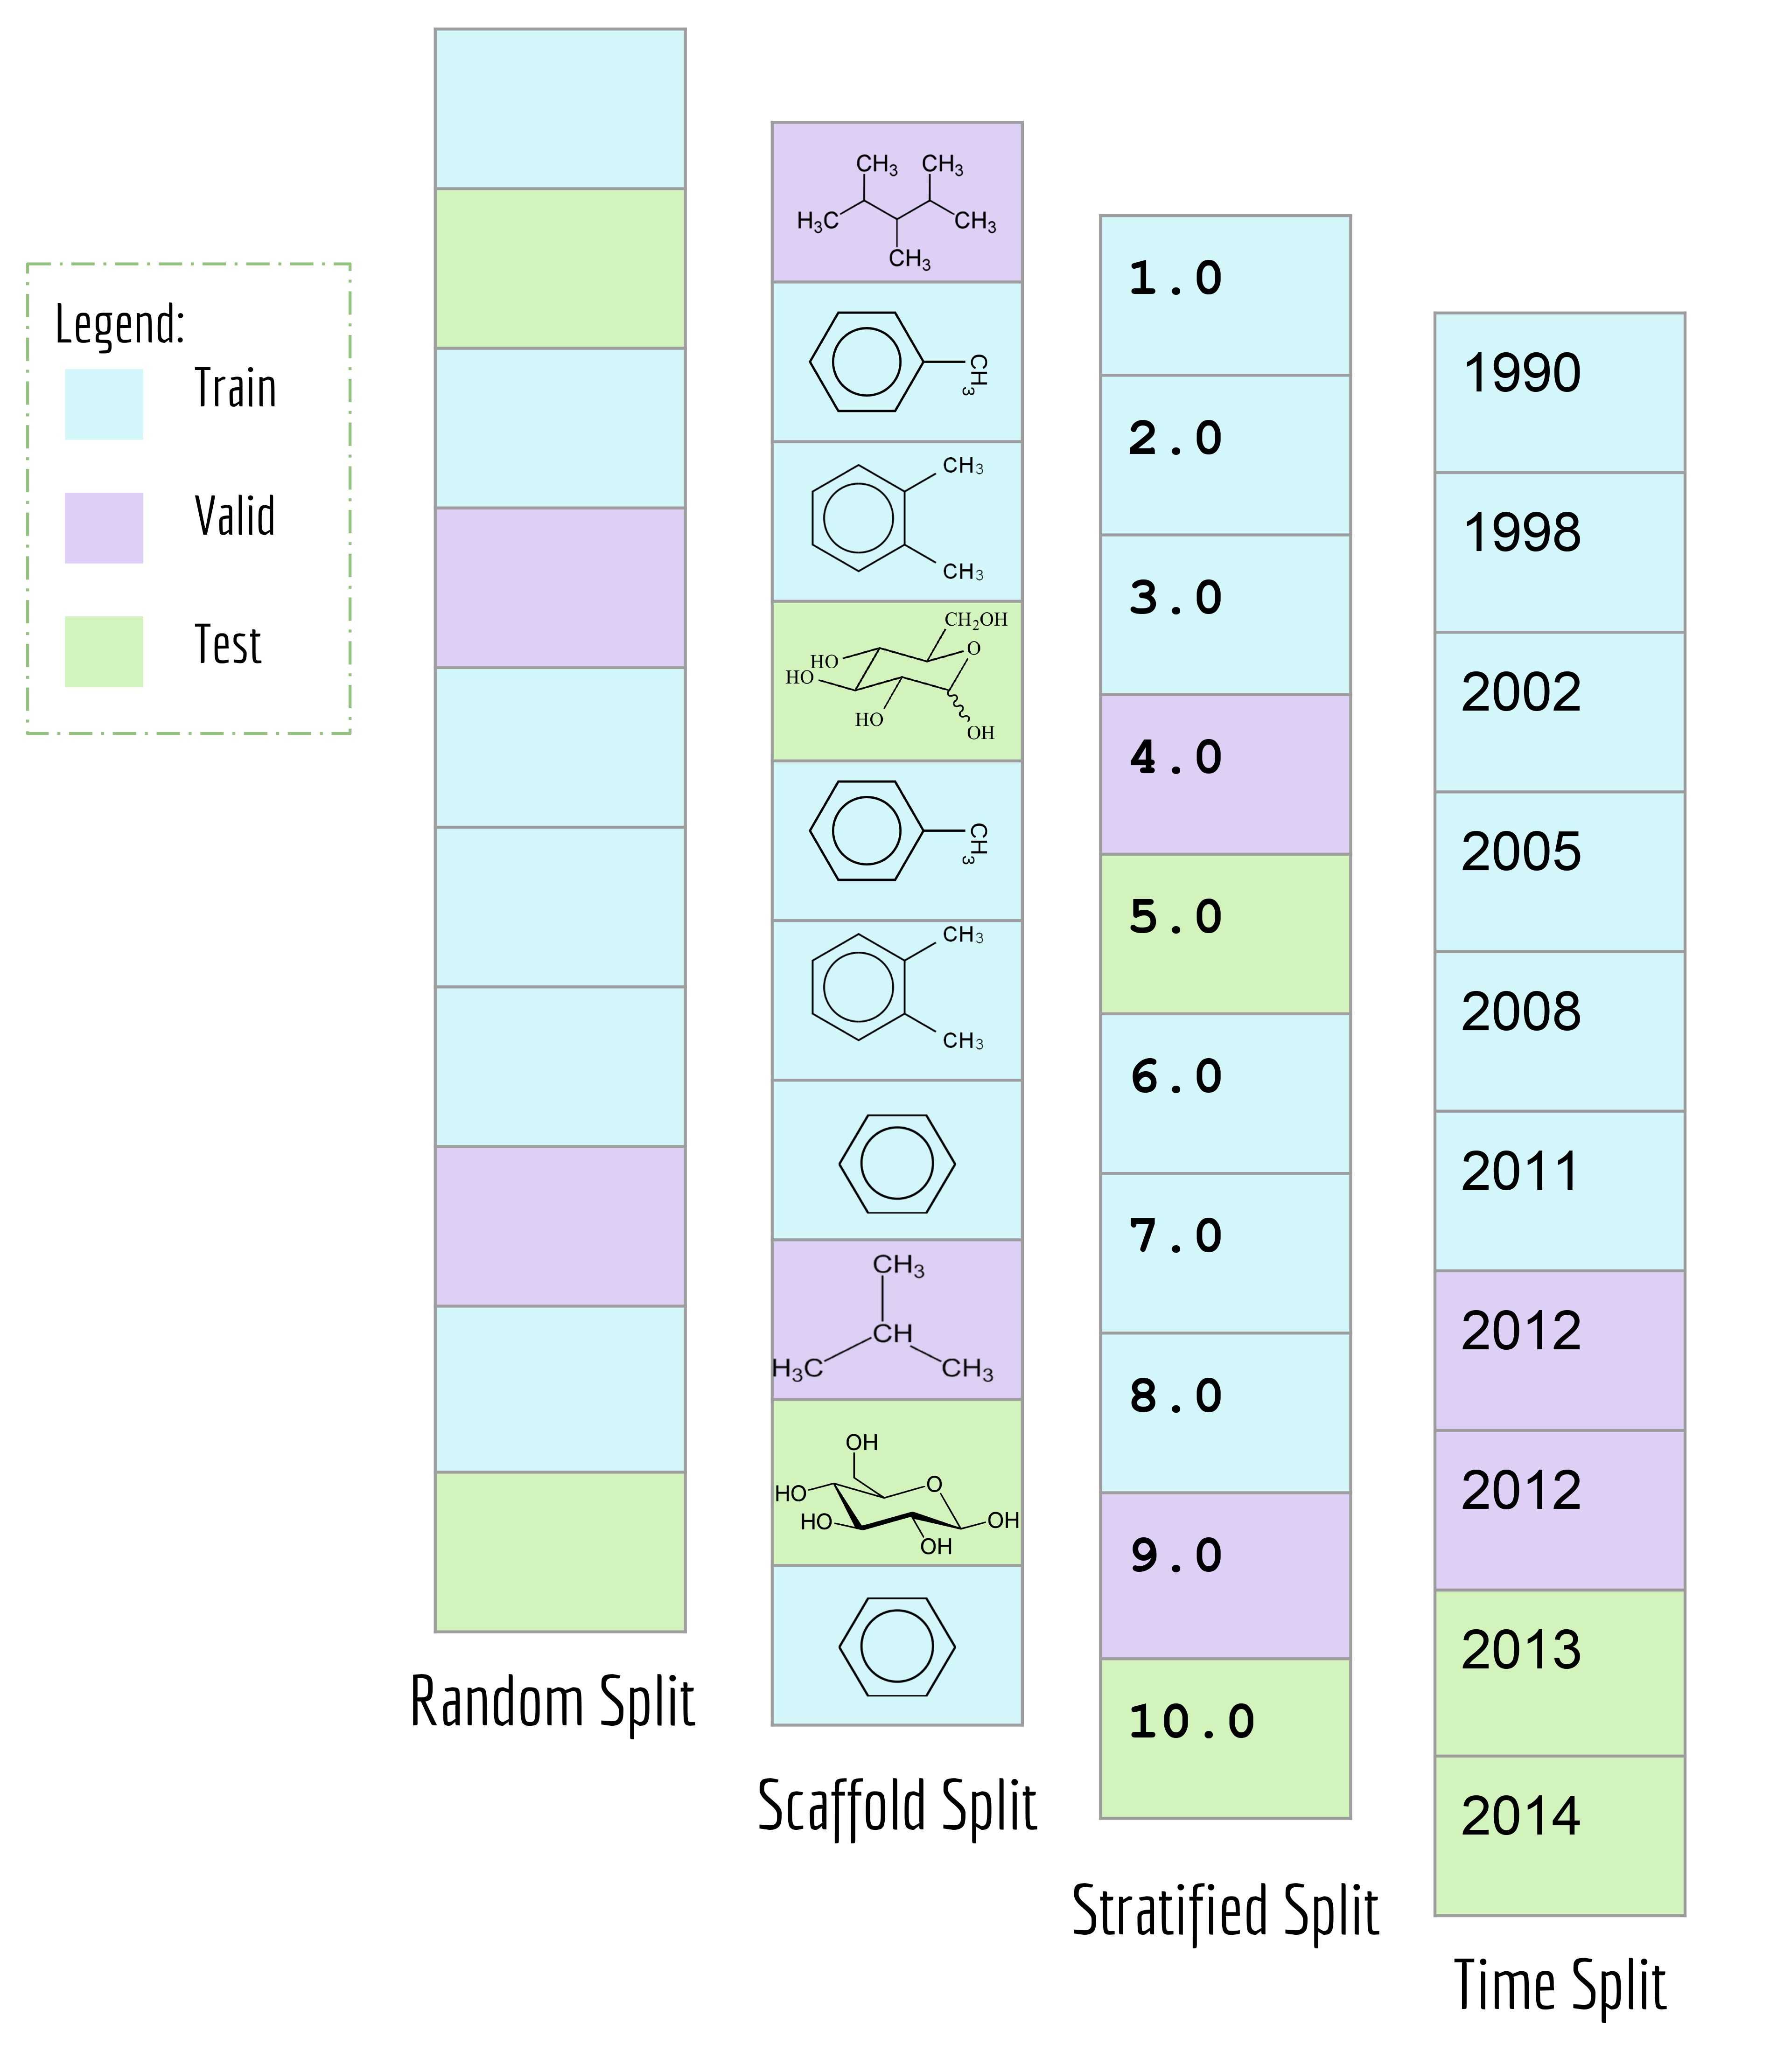
\includegraphics[width=0.4\textwidth]{Images/molnet_splits.png}
  \caption{Representation of Data Splits in MoleculeNet.}
  \label{fig:data_splits}
\end{figure}

As mentioned previously, random splitting of molecular data isn't always best for evaluating machine learning methods. Consequently, MoleculeNet implements multiple different splittings for each dataset. Random splitting randomly splits samples into the training/validation/test subsets. Scaffold splitting splits the samples based on their two-dimensional structural frameworks,\cite{scaffold} as implemented in RDKit.\cite{RDKit} Since scaffold splitting attempts to separate structurally different molecules into different subsets, it offers a greater challenge for learning algorithms than the random split.

In addition, a stratified random sampling method is implemented on the QM7 dataset to reproduce the results from the original work.\cite{GDB7_dataset_arxiv} This method sorts datapoints in order of increasing label value (note this is only defined for real-valued output). This sorted list is then split into training/validation/test by ensuring that each set contains the full range of provided labels. Time splitting is also adopted for dataset that includes time information(PDBbind). Under this splitting method, model will be trained on older data and tested on newer data, mimicing real world development condition.

MoleculeNet contributes the code for these splitting methods into DeepChem. Users of the library can use these splits on new datasets with short library calls.


\subsubsection{Metrics}

MoleculeNet contains both regression datasets (QM7, QM7b, QM8, QM9, ESOL, FreeSolv, Lipophilicity and PDBbind) and classification datasets (PCBA, MUV, HIV, BACE, BBBP, Tox21, ToxCast and SIDER). Consequently, different performance metrics need to be measured for each. Following suggestions from the community\cite{metric_suggestion}, regression datasets are evaluated by mean absolute error (MAE) and root-mean-square error (RMSE), classification datasets are evaluated by area under curve (AUC) of the receiver operating characteristic (ROC) curve\cite{AUC-ROC} and the precision recall curve (PRC)\cite{PRC}. For datasets containing more than one task, we report the mean metric values over all tasks.

\begin{figure}[!h]
  \centering
  \small
  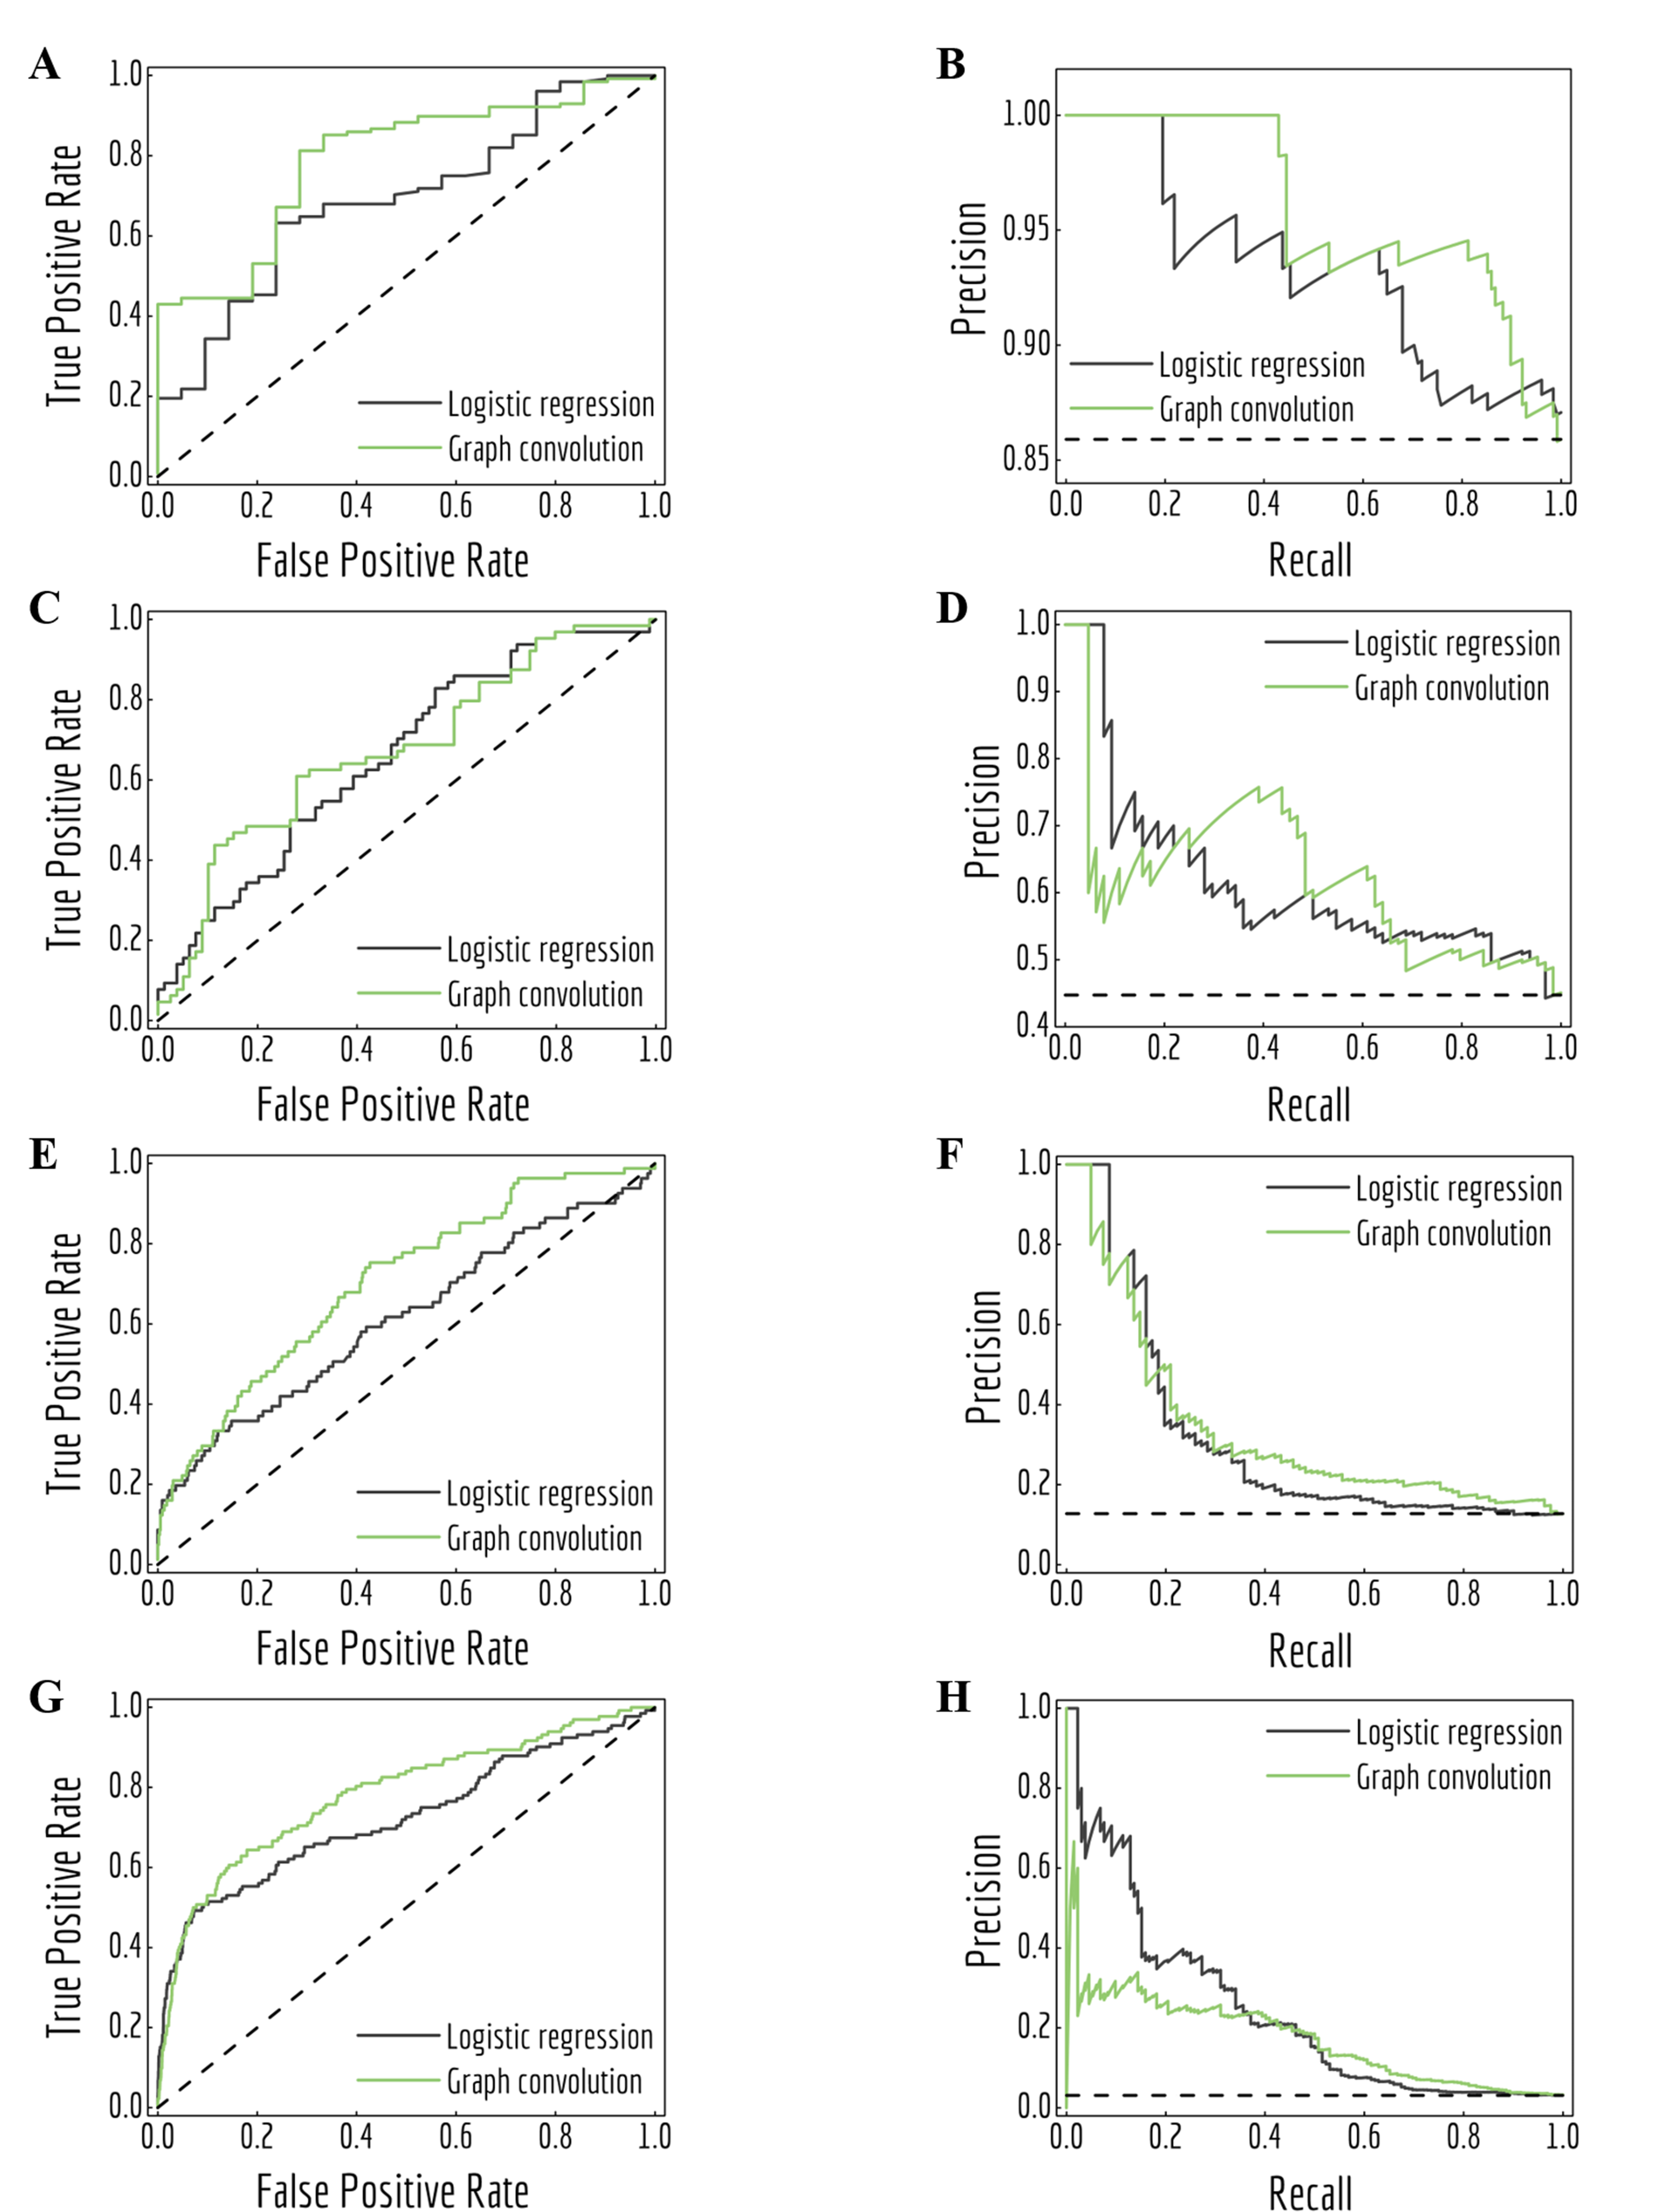
\includegraphics[width=0.45\textwidth]{Images/ROCvsPRC.png}
  \caption{Receiver operating characteristic (ROC) curves and precision recall curves (PRC) for predictions of logistic regression and graph convolutional models under different class imbalance condition.(Details listed in Table~\ref{tab:ROCvsPRC_AUC}): \textbf{A, B}: task "FDA\_APPROVED" from ClinTox, test subset; \textbf{C, D}: task "Hepatobiliary disorders" from SIDER, test subset; \textbf{E, F}: task "NR-ER" from Tox21, validation subset; \textbf{G, H}: task "HIV\_active" from HIV, test subset. Black dashed lines are performances of random classifiers.}
  \label{fig:ROCvsPRC}
\end{figure}

\begin{table}[h]
    \small
    \caption{Task details and area under curve(AUC) values of sample curves}
    \label{tab:ROCvsPRC_AUC}
    \begin{tabular*}{0.5\textwidth}{@{\extracolsep{\fill}}lllll}
    \hline
    \textbf{Task} & \textbf{P/N}* & \textbf{Model} & \textbf{ROC} & \textbf{PRC}\\ 
    \hline
    \multirow{2}{*}{\tabincell{l}{``FDA\_APPROVED''\\ClinTox, test subset}} &  \multirow{2}{*}{128/21} &{\scriptsize Logistic Regression} & 0.691 & 0.932 \\\cline{3-5}
    & & {\scriptsize Graph Convolution} & 0.791 & 0.959 \\
    \hline
    \multirow{2}{*}{\tabincell{l}{``Hepatobiliary disorders''\\SIDER, test subset}} &  \multirow{2}{*}{64/79} & {\scriptsize Logistic Regression} & 0.659 & 0.612 \\\cline{3-5}
    & & {\scriptsize Graph Convolution} & 0.675 & 0.620 \\
    \hline
    \multirow{2}{*}{\tabincell{l}{``NR-ER''\\Tox21, valid subset}} &  \multirow{2}{*}{81/553} & {\scriptsize Logistic Regression} & 0.612 & 0.308 \\\cline{3-5}
    & & {\scriptsize Graph Convolution} & 0.705 & 0.333 \\
    \hline
    \multirow{2}{*}{\tabincell{l}{``HIV\_active''\\HIV, test subset}} &  \multirow{2}{*}{132/4059} & {\scriptsize Logistic Regression} & 0.724 & 0.236 \\\cline{3-5}
    & & {\scriptsize Graph Convolution} & 0.783 & 0.169 \\
    \hline
    \end{tabular*}
    \begin{tablenotes}
    \item * Number of positive samples/Number of negative samples
    \end{tablenotes}
\end{table}

To allow better comparison, we propose regression metrics according to previous work on either same models or datasets. For classification datasets, we propose recommended metrics from the two commonly used metrics: AUC-PRC and AUC-ROC. Four representative sets of ROC curves and PRCs are depicted in Figure~\ref{fig:ROCvsPRC}, resulting from the predictions of logistic regression and graph convolutional models on four tasks. Details about these tasks and AUC values of all curves are listed in Table~\ref{tab:ROCvsPRC_AUC}. Note that these four tasks have different class imbalances, represented as the number of positive samples and negative samples.

As noted in previous literature\cite{PRC}, ROC curves and PRCs are highly correlated, but perform significantly differently in case of high class imbalance. As shown in Figure~\ref{fig:ROCvsPRC}, the fraction of positive samples decreases from over 80\% (panels A and B) to less than 5\% (panels G and H). This change accompanies the difference in how the two metrics treat model performances. In particular, PRCs put more emphasis on the low recall (also known as true positive rate (TPR)) side in case of highly imbalanced data: logistic regression slightly outperforms graph convolutional models in the low TPR side of ROC curves (panels C, E and G, lower left corner), which creates different margins on the low recall side of PRCs.

ROC curves and PRCs share one same axis, while using false positive rate (FPR) and precision for the other axis respectively. Recall that FPR and precision are defined as follows:
\begin{equation*}
    \small
    FPR=\frac{\rm{False\,Positive}}{\rm{False\,Positive} + \rm{True\,Negative}}
\end{equation*}
\begin{equation*}
    \small
    Precision=\frac{\rm{True\,Positive}}{\rm{False\,Positive} + \rm{True\,Positive}}
\end{equation*}

When positive samples form only a small proportion of all samples, false positive predictions exert a much greater influence on precision than FPR, amplifying the difference between PRC and ROC curves. Virtual screening experiments do have extremely low positive rates, suggesting that the correct metric to analyze may depend on the experiment at hand. In this work, we hence propose recommended metrics based on positive rates, PRC-AUC is used for datasets with positive rates less than 2\%, otherwise ROC-AUC is used. 


\subsubsection{Featurization}

A core challenge for molecular machine learning is effectively encoding molecules into fixed-length strings or vectors. Although SMILES strings are unique representations of molecules, most molecular machine learning methods require further information to learn sophisticated electronic or topological features of molecules from limited amounts of data. (Recent work has demonstrated the ability to learn useful representations from SMILES strings using more sophisticated methods\cite{gomez2016automatic}, so it may be feasible to use SMILES strings for further learning tasks in the near future.) Furthermore, the enormity of chemical space often requires representations of molecules specifically suited to the learning task at hand. MoleculeNet contains implementations of six useful molecular featurization methods.

\begin{figure}[h]
  \centering
  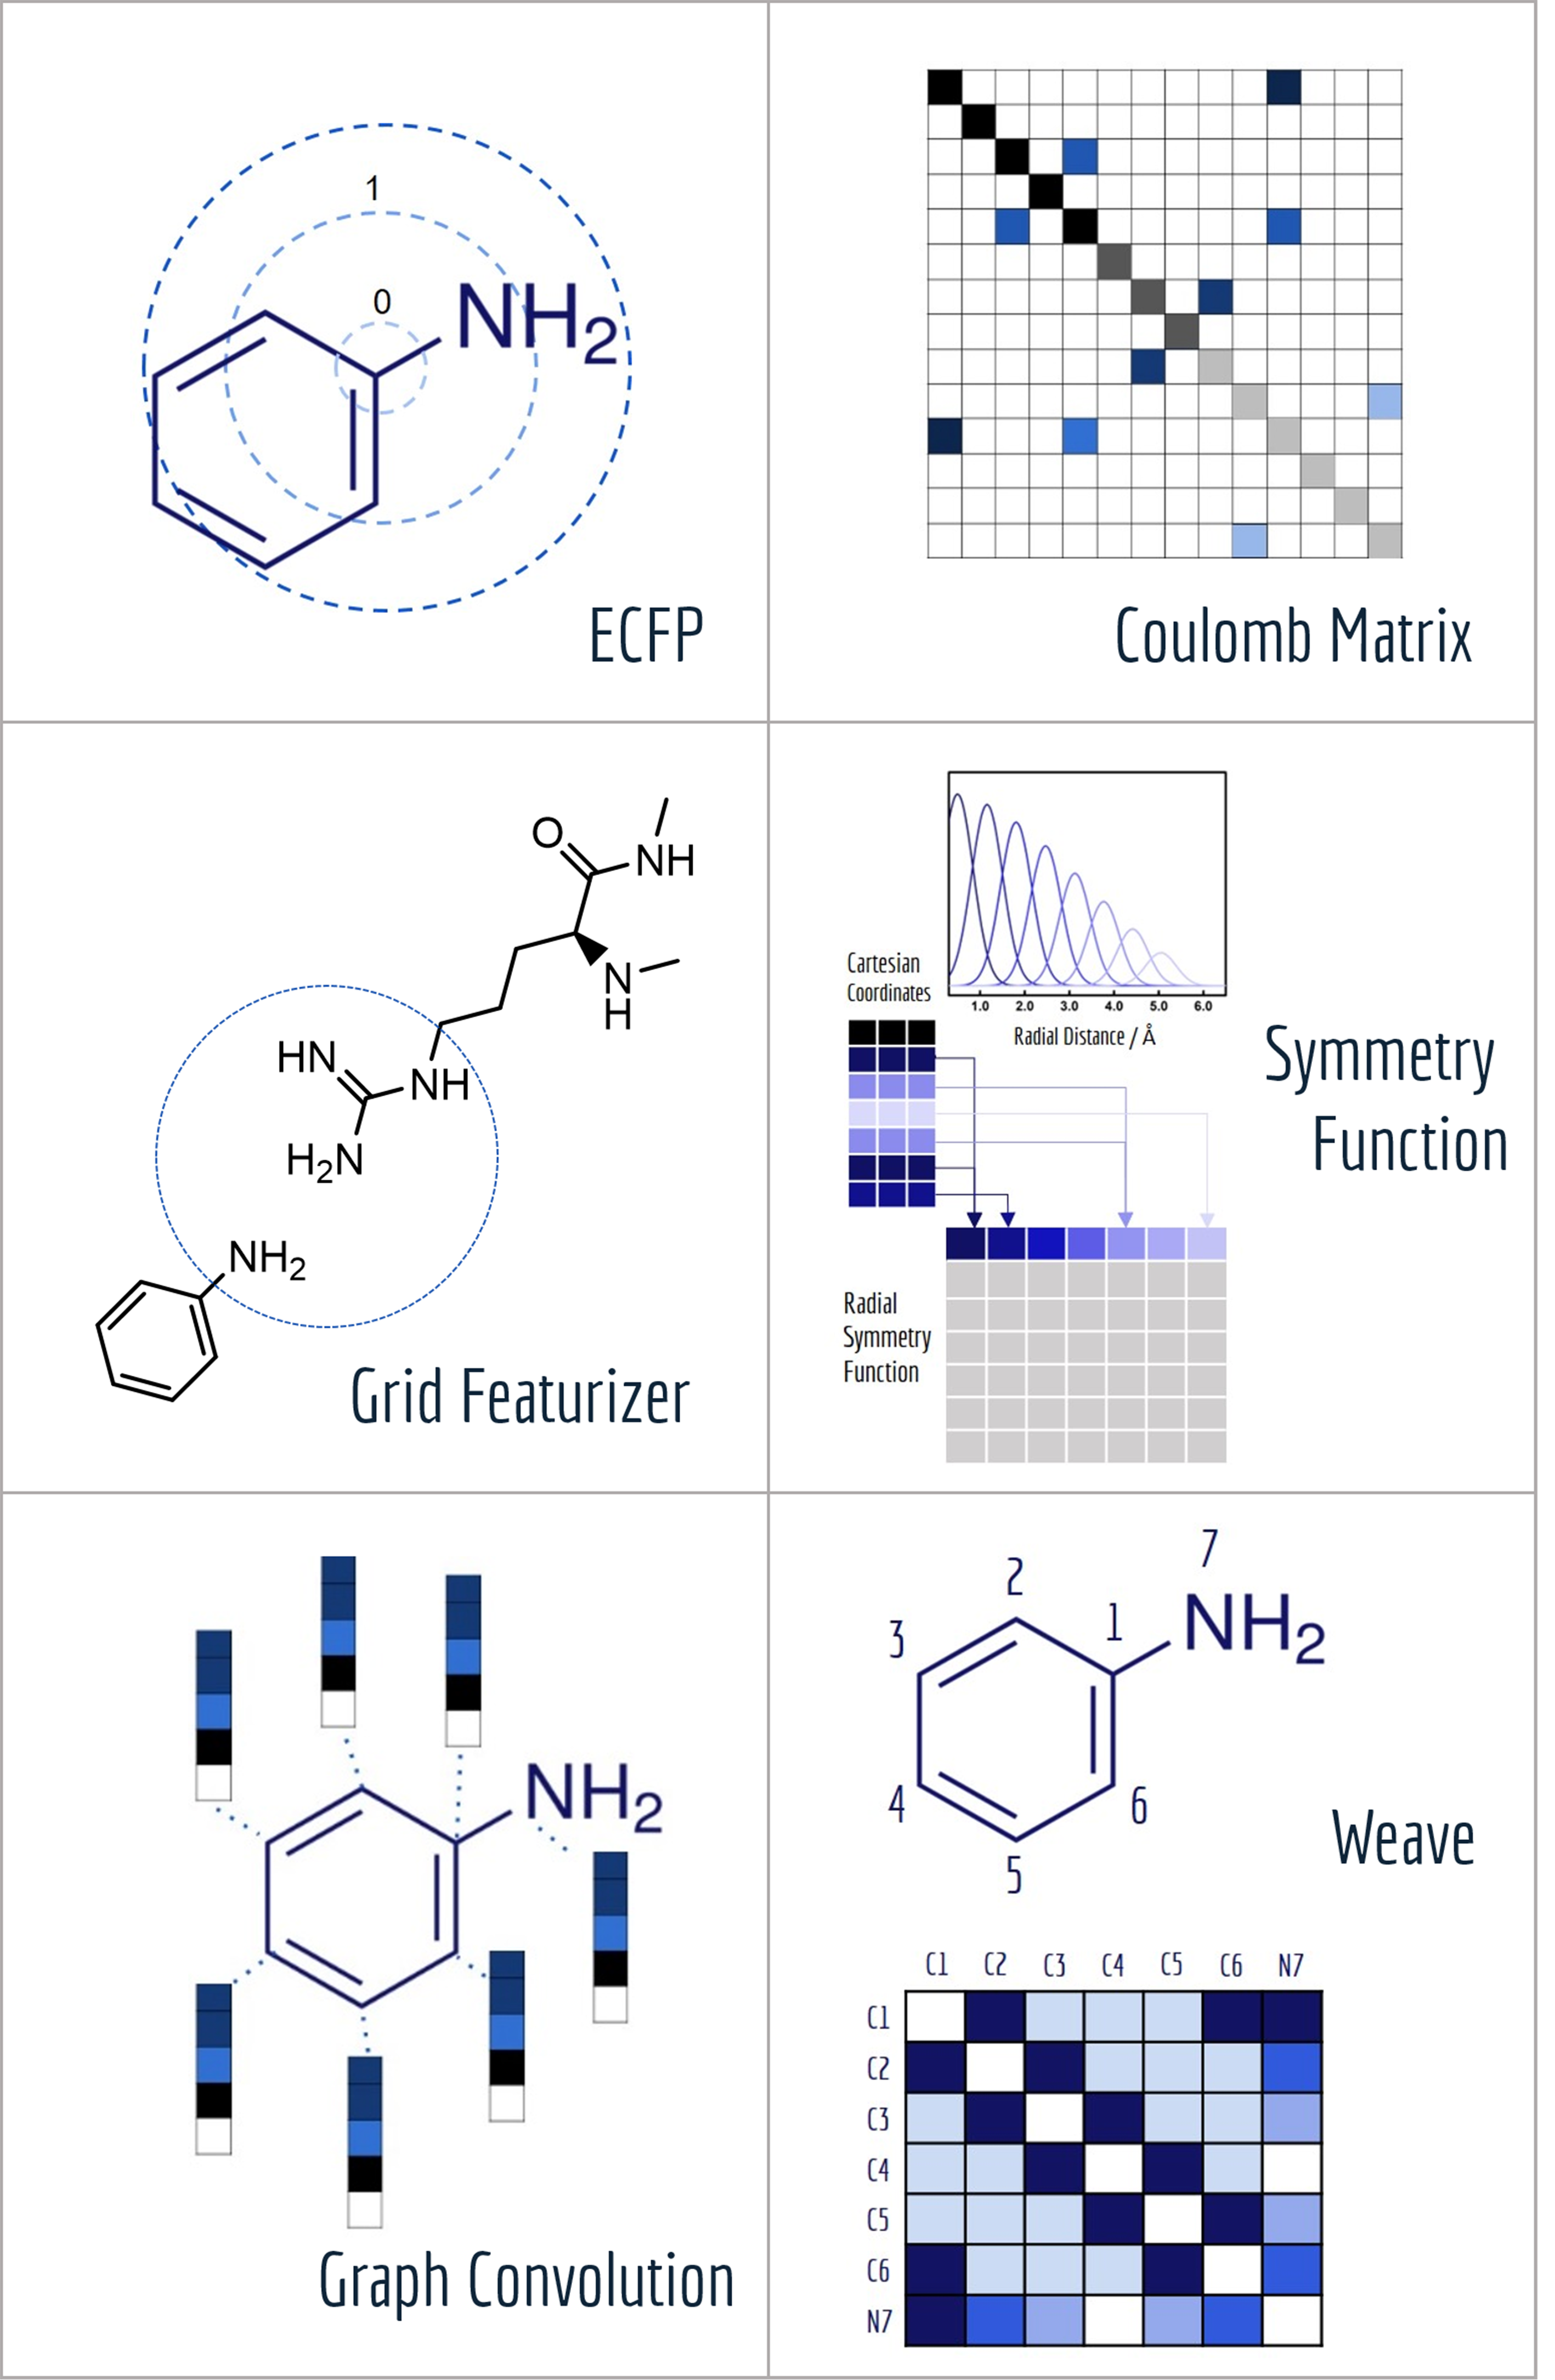
\includegraphics[width=.45\textwidth]{Images/molnet_feat.png}
  \caption{Diagrams of featurizations in MoleculeNet.}
  \label{fig:molnet_feat}
\end{figure}

\paragraph{ECFP}

Extended-Connectivity Fingerprints (ECFP) are widely-used molecular characterizations in chemical informatics.\cite{ECFP} During the featurization process, a molecule is decomposed into submodules originated from heavy atoms, each assigned with a unique identifier. These segments and identifiers are extended through bonds to generate larger substructures and corresponding identifiers.

After hashing all these substructures into a fixed length binary fingerprint, the representation contains information about topological characteristics of the molecule, which enables it to be applied to tasks such as similarity searching and activity prediction. The MoleculeNet implementation uses ECFP4 fingerprints generated by RDKit.\cite{RDKit}

\paragraph{Coulomb Matrix}

\textit{Ab-initio} electronic structure calculations typically require a set of nuclear charges \{\textit{Z}\} and the corresponding Cartesian coordinates \{\textbf{R}\} as input.  The Coulomb Matrix (CM) \textbf{M}, proposed by Rupp et al.\cite{GDB7_dataset_prl} and defined below, encodes this information by use of the atomic self-energies and internuclear Coulomb repulsion operator.

\begin{eqnarray*}
    M_{IJ}=
    \begin{cases}
    0.5Z_I^{2.4}\qquad\mbox{for}\;I=J \\
    \frac{Z_IZ_J}{|\bm{R}_I-\bm{R}_J|}\qquad\mbox{for}\;I\neq J
    \end{cases}
\end{eqnarray*}

Here, the off-diagonal elements correspond to the Coulomb repulsion between atoms I and J, and the diagonal elements correspond to a polynomial fit of atomic self-energy to nuclear charge.  The Coulomb Matrix of a molecule is invariant to translation and rotation of that molecule, but not with respect to atom index permutation.  In the construction of coulomb matrix, we first use the nuclear charges and distance matrix generated by RDKit\cite{RDKit} to acquire the original coulomb matrix, then an optional random atom index sorting and binary expansion transformation can be applied during training in order to achieve atom index invariance, as reported by Montavon et al.\cite{GDB7_dataset_arxiv}

\paragraph{Grid Featurizer}

The grid featurizer is a featurization method (introduced in the current work) initially designed for the PDBBind dataset in which structural information of both the ligand and target protein are considered. Since binding affinity stems largely from the intermolecular forces between ligands and proteins, in addition to intramolecular interactions, we seek to incorporate both the chemical interaction within the binding pocket as well as features of the protein and ligand individually.

The grid featurizer was inspired by the NNscore featurizer \cite{NNscore} and SPLIF \cite{da2014structural} but optimized for speed, robustness, and generalizability. The intermolecular interactions enumerated by the featurizer include salt bridges and hydrogen bonding between protein and ligand, intra-ligand circular fingerprints, intra-protein circular fingerprints, and protein-ligand SPLIF fingerprints. A more detailed breakdown can be found in the supplementary information\dag.


%Although the original NNScore featurizer includes $\pi$-bond interactions, we found that including these interactions didn't improve the quality of our results (perhaps due to the difficulty of correctly detecting $\pi$-interactions with hand-encoded rules).
%ENF: I don't see the need to mention the $\pi$ interactions here if we ultimately are not including them in V1 of the paper.

\paragraph{Symmetry Function}

Symmetry function, first introduced by Behler and Parrinello\cite{SymmetryFunction}, is another common encoding of atomic coordinates information. It focuses on preserving the rotational and permutation symmetry of the system. The local environment of an atom in the molecule is expressed as a series of radial and angular symmetry functions  with different distance and angle cutoffs, the former focusing on distance between atom pairs and the latter focusing on angles formed within triplets of atoms. 

As symmetry function put most emphasis on spatial positions of atoms, it is intrinsically hard for it to distinguish different atom types(H, C, O). MoleculeNet utilizes a slightly modified version of original symmetry function\cite{ANI-1} which further separate radial and angular symmetry terms according to the type of atoms in the pair or triplet. Further details can be found in the article\cite{ANI-1} or our implementation.


\paragraph{Graph Convolutions}

The graph convolutions featurization support most graph-based models. It computes an initial feature vector and a neighbor list for each atom. The feature vector summarizes the atom's local chemical environment, including atom-types, hybridization types, and valence structures. Neighbor lists represent connectivity of the whole molecule, which are further processed in each model to generate graph structures (discussed in further details in following parts).

\paragraph{Weave}

Similar to graph convolutions, the weave featurization encodes both local chemical environment and connectivity of atoms in a molecule. Atomic feature vectors are exactly the same, while connectivity uses more detailed pair features instead of neighbor listing. The weave featurization calculates a feature vector for each pair of atoms in the molecule, including bond properties (if directly connected), graph distance and ring info, forming a feature matrix. The method supports graph-based models that utilize properties of both nodes (atoms) and edges (bonds).

\subsubsection{Models - Conventional Models}

MoleculeNet tests the performance of various machine learning models on the datasets discussed previously. These models could be further categorized into conventional method and graph-based method according to their structures and input types. The following sections will give brief introductions to benchmarked algorithms. The results section will discuss performance numbers in detail. Here we briefly review conventional methods including logistic regression, support vector classification, kernel ridge regression, random forests\cite{breiman2001random}, gradient boosting\cite{friedman2001greedy}, multitask networks\cite{ramsundar2015massively, ma2015deep}, bypass networks \cite{Bypass_network} and influence relevance voting\cite{IRV}. The next section graph-based models will give introductions to graph convolutional models\cite{graphconv_feat}, weave models\cite{kearnes2016graphconv}, directed acyclic graph models\cite{lusci2013deep}, deep tensor neural networks\cite{schutt2016quantum}, ANI-1\cite{ANI-1} and message passing neural networks\cite{MPNN}. As part of this work, all methods are implemented in the open source DeepChem package\cite{deepchem}.

\paragraph{Logistic Regression}

Logistic regression models (Logreg) apply the logistic function to weighted linear combinations of their input features to obtain model predictions. It is often common to use regularization to encourage learned weights to be sparse. \cite{friedman2000additive} Note that logistic regression models are only defined for classification tasks.

\paragraph{Support Vector Classification}

Support vector machine (SVM) is one of the most famous and widely-used machine learning method.\cite{cortes1995support} As in classification task, it defines a decision plane which separates data points of different class with maximized margin. To further increase performance, we incorporates regularization and a radial basis function kernel (KernelSVM).

\paragraph{Kernel Ridge Regression}

Kernel ridge regression(KRR) is a combination of ridge regression and kernel trick. By using a nonlinear kernel function(radial basis function), it learns a non-linear function in the original space that maps features to predicted values.

\paragraph{Random Forests}

Random forests (RF) are ensemble prediction methods.\cite{breiman2001random} A random forest consists of many individual decision trees, each of which is trained on a subsampled version of the original dataset. The results for individual trees are averaged to provide output predictions for the full forest. Random forests can be used for both classification and regression tasks. Training a random forest can be computationally intensive, so benchmarks only include random forest results for smaller datasets.

\paragraph{Gradient Boosting}

Gradient boosting is another ensemble method consisting of individual decision trees.\cite{friedman2001greedy} In contrast to random forests, it builds relatively simple trees which are sequentially incorporated to the ensemble. In each step, a new tree is generated in a greedy manner to minimize loss function. A sequence of such "weak" trees are combined together into an additive model. We utilize the XGBoost implementation of gradient boosting in DeepChem.\cite{XGBoost}

\paragraph{Multitask/Singletask Network}

In a multitask network,\cite{ramsundar2015massively} input featurizations are processed by fully connected neural network layers. The processed output is shared among all learning tasks in a dataset, and then fed into separate linear classifiers/regressors for each different task. In the case that a dataset contains only a single task, multitask networks are just fully connected neural networks(Singletask Network). Since multitask networks are trained on the joint data available for various tasks, the parameters of the shared layers are encouraged to produce a joint representation which can share information between learning tasks. This effect does seem to have limitations; merging data from uncorrelated tasks has only moderate effect.\cite{kearnes2016modeling} As a result, MoleculeNet does not attempt to train extremely large multitask networks combining all data for all datasets.

\paragraph{Bypass Multitask Networks}

Multitask modeling relies on the fact that some features have explanatory power that is shared among multiple tasks. Note that the opposite may well be true; features useful for one task can be detrimental to other tasks. As a result, vanilla multitask networks can lack the power to explain unrelated variations in the samples. Bypass networks attempt to overcome this variation by merging in per-task independent layers that ``bypass'' shared layers to directly connect inputs with outputs.\cite{Bypass_network} In other words, bypass multitask networks consist of $n_\text{tasks}+1$ independent components: one ``multitask'' layers mapping all inputs to shared representations, and $n_\text{tasks}$ ``bypass'' layers mapping inputs for each specific task to their labels. As the two groups have separate parameters, bypass networks may have greater explanatory power than vanilla multitask networks.

\paragraph{Influence Relevance Voting}

Influence Relevance Voting (IRV) systems are refined K-nearest neighbour classifiers.\cite{IRV} Using the hypothesis that compounds with similar substructures have similar functionality, the IRV classifier makes its prediction by combining labels from the top-$K$ compounds most similar to a provided test sample.

The Jaccard-Tanimoto similarity between fingerprints of compounds is used as the similarity measurement:

\begin{equation*}
    S(\vec{A},\vec{B})=
    \frac{A\cap B}{A\cup B}
\end{equation*}

Then IRV model calculates a weighted sum of labels of top K similar compounds to predict the result, in which weights are the outputs of a one-hidden layer neural network with similarities and rankings of top-$K$ compounds as input. Detailed descriptions of the model can be found in the original article.\cite{IRV} 

\subsubsection{Models - Graph Based Models}

Early attempts to directly use molecular structures instead of selected features has emerged in 1990s\cite{baskin1997neural, kireev1995chemnet}. While in recent years, models propelled by the very similar idea start to grow rapidly. These specifically designed methods, namely graph-based models, are naturally suitable for modelling molecules. By defining atoms as nodes, bonds as edges, molecules can be modeled as mathematical graphs. As noted in a recent paper\cite{MPNN}, this natural similarity has inspired a number of models to utilize the graph structure of molecules to gain higher performances. In general, graph-based models apply adaptive functions to nodes and edges, allowing for a learnable featurization process. MoleculeNet provides implementations of multiple graph-based models which use different variants of molecular graphs. Figure~\ref{fig:model_structure1} provide simple illustrations of these methods' core structures. We describe these methods in details in the following sections. To further validate the model implementations, we compare the performances of these models with their original sources, results can be found in the supplementary information.\dag

\begin{figure*}
  \centering
  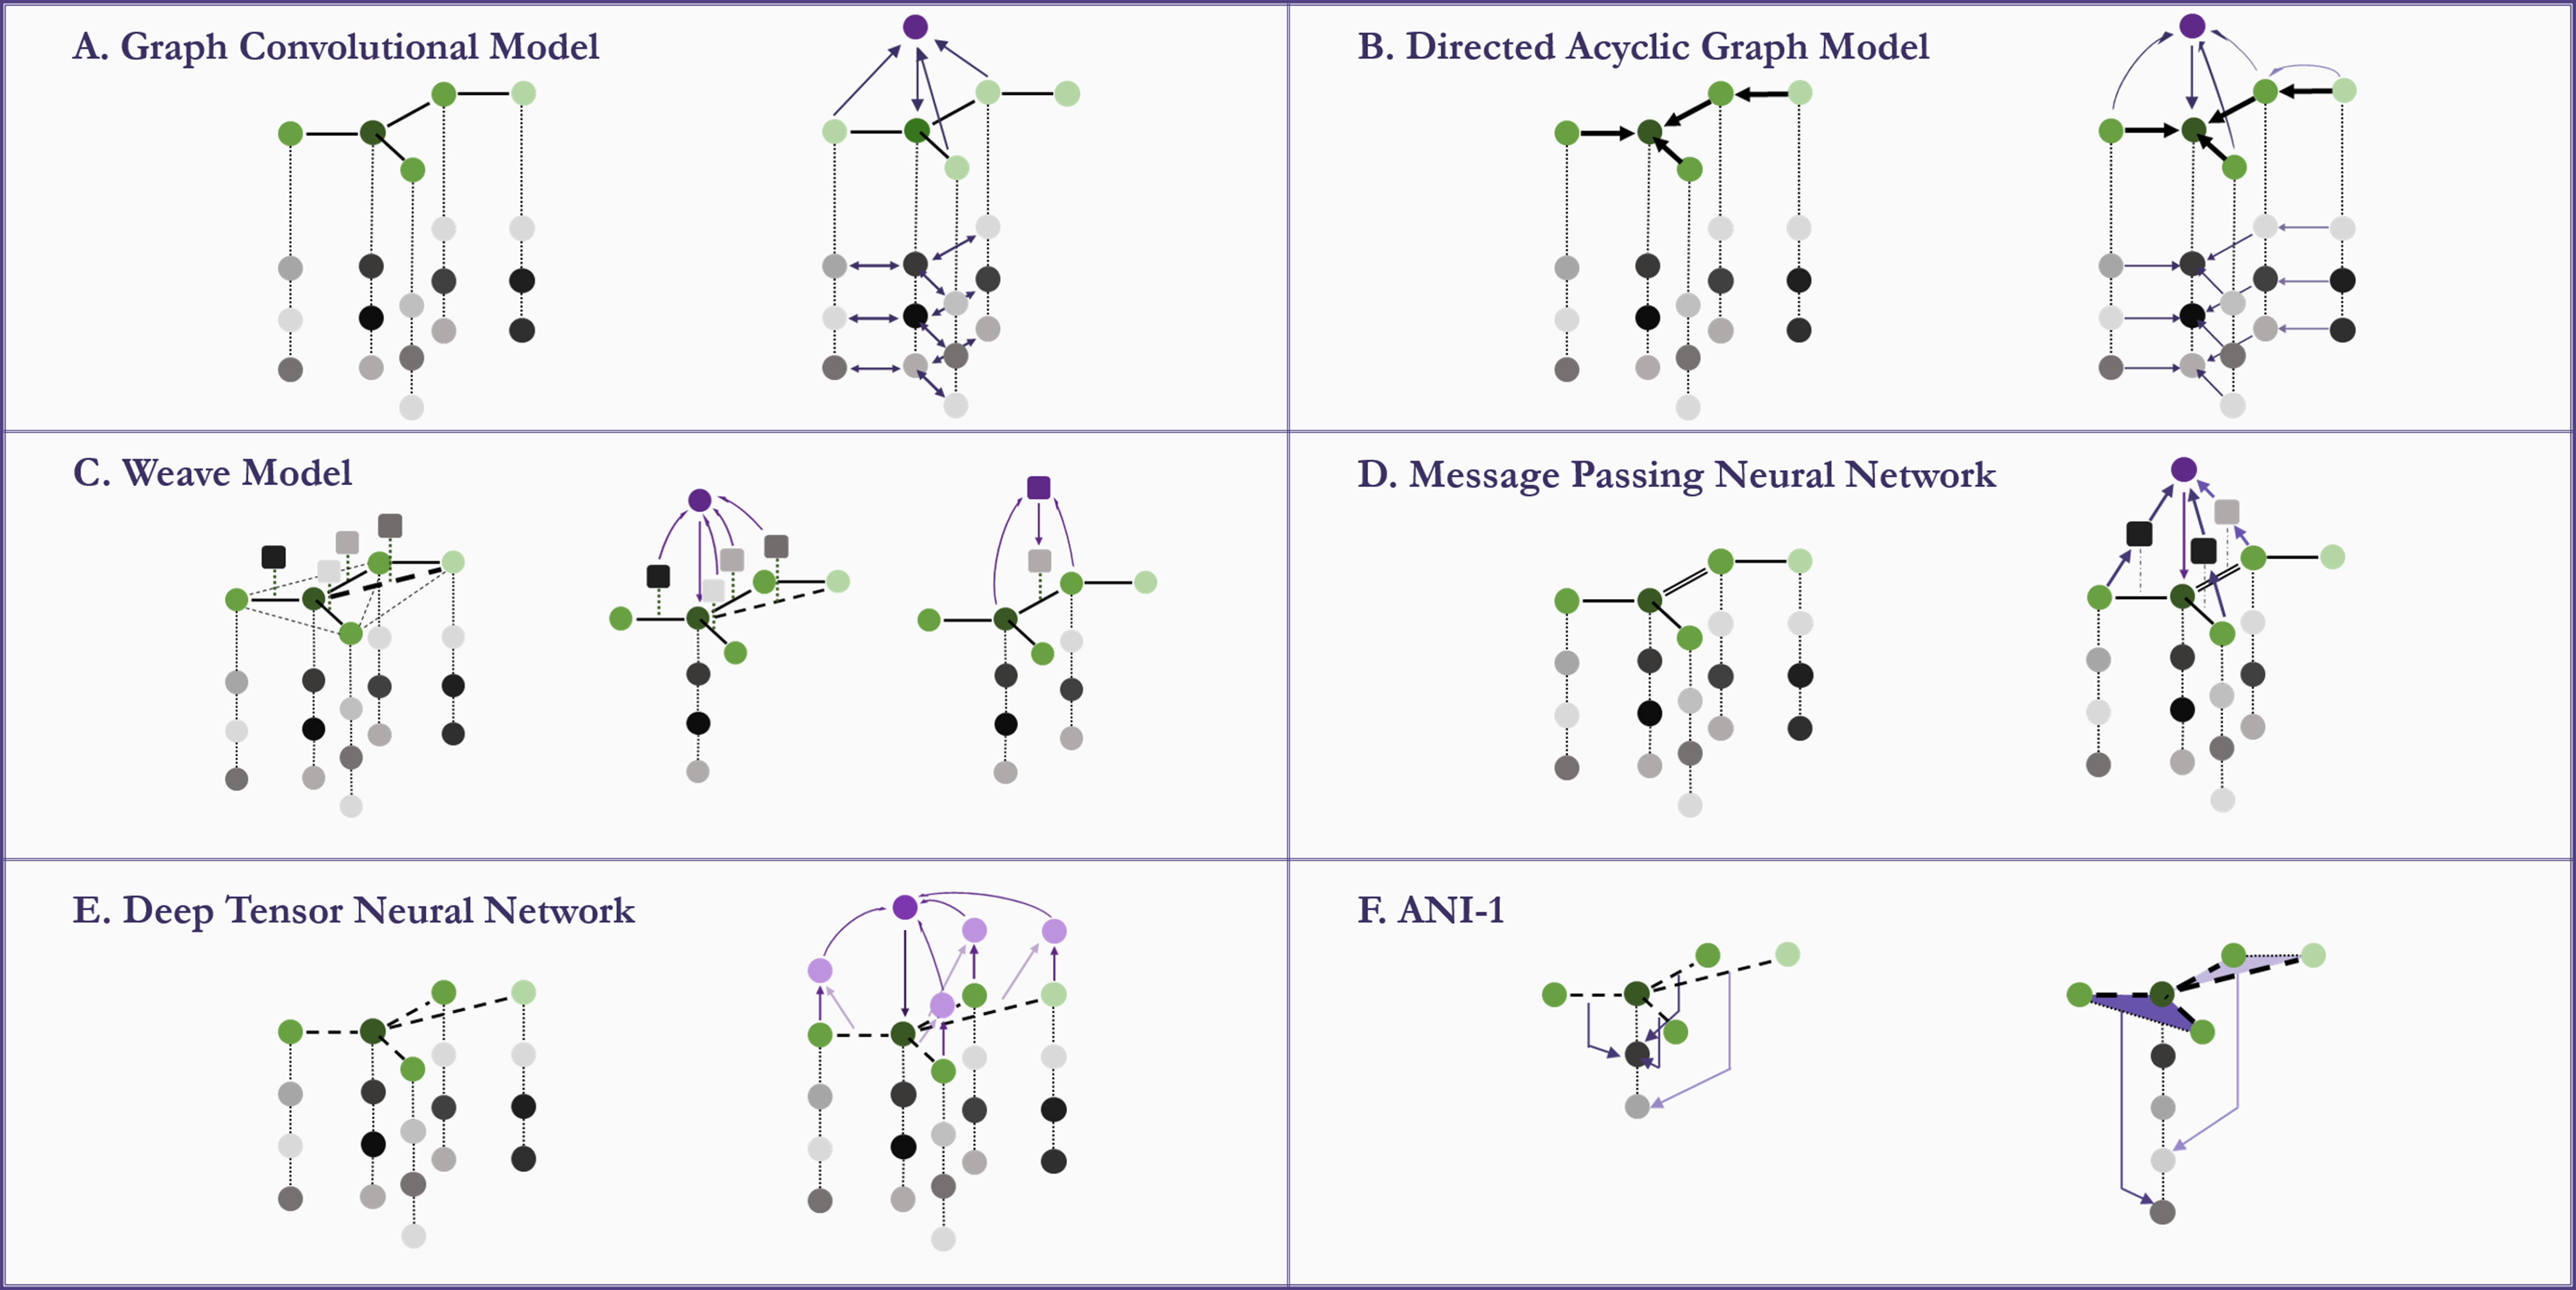
\includegraphics[width=0.9\textwidth]{Images/model_structure.png}
  \caption{Core structures of graph-based models implemented in MoleculeNet. To build features for the central dark green atom: \textbf{A} Graph Convolutional Model: features are updated by combination with neighbour atoms; \textbf{B} Directed Acyclic Graph Model: all bonds are directed towards the central atom, features are propagated from the farthest atom to the central atom through directed bonds; \textbf{C} Weave Model: Pairs are formed between each pair of atoms(including not directly bonded pairs), features for the central atom are updated using all other atoms and their corresponding pairs, pair features are also updated by combination of the two pairing atoms; \textbf{D} Message Passing Neural Network: Neighbour atoms' features are input into bondtype-dependent neural networks, forming outputs(messages). Features of the central atom are then updated using the outputs; \textbf{E} Deep Tensor Neural Network: No explicit bonding information is included, features are updated using all other atoms based on their corresponding physical distances; \textbf{F} ANI-1: features are built on distance information between pairs of atoms(radial symmetry functions) and angular information between triplets of atoms(angular symmetry functions).}
  \label{fig:model_structure1}
\end{figure*}

\paragraph{Graph Convolutional models}

Graph convolutional models (GC) extend the decomposition principles of circular fingerprints. Both methods gradually merge information for distant atoms by extending radially through bonds. This information is used to generate identifiers for all substructures. However, instead of applying fixed hash functions, graph convolutional models allow for adaptive learning by using differentiable network layers. This creates a learnable process capable of extracting useful representations of molecules suited to the task at hand. (Note that this property is shared, to some degree, by all deep architectures considered in MoleculeNet. However, graph convolutional architectures are more explicitly designed to encourage extraction of useful featurizations).

On a higher level, graph convolutional models treat molecules as undirected graphs, and apply the same learnable function to every node (atom) and its neighbors (bonded atoms) in the graph. This structure recapitulates convolution layers in visual recognition deep networks.

MoleculeNet uses the graph convolutional implementation in DeepChem from previous work.\cite{altae2016low} This implementation converts SMILES strings into molecular graphs using RDKit \cite{RDKit} As mentioned previously, the initial representations assign to each atom a vector of features including its element, connectivity, valence, etc. Then several graph convolutional modules, each consisting of a graph convolutional layer, a batch normalization layer and a graph pool layer, are sequentially added, followed by a fully-connected dense layer. Finally, the feature vectors for all nodes (atoms) are summed, generating a graph feature vector, which is fed to a classification or regression layer.

\paragraph{Weave models}

The Weave architecture is another graph-based model that regards each molecule as a undirected graph. Similar to graph convolutional models, it utilizes the idea of adaptive learning on extracting meaningful representations.\cite{kearnes2016graphconv} The major difference is the size of the convolutions: To update features of an atom, weave models combine info from all other atoms and their corresponding pairs in the molecule. Weave models are more efficient at transmitting information between distant atoms, at the price of increased complexity for each convolution.

In our implementation, a molecule is first encoded into a list of atomic features and a matrix of pair features by the weave model's featurization method. Then in each weave module, these features are inputted into four sets of fully connected layers (corresponding to four paths from two original features to two updated features) and concatenated to form new atomic and pair features. After stacking several weave modules, a similar gather layer combines atomic features together to form molecular features that are fed into task-specific layers.

\paragraph{Directed Acyclic Graph models}

Directed Acyclic Graph (DAG) models regard molecules as directed graphs. While chemical bonds typically do not have natural directions, one can arbitrarily generate a DAG on a molecule by designating a central atom and then define directions of all bonds in certain orientations towards the atom.\cite{lusci2013deep} In the case of small molecules, taking all possible orientations is computationally feasible. In other words, for a molecule with $n_a$ atoms, the model will generate $n_a$ DAGs, each centered on a different atom. 

In the actual calculations of a graph, a vector of graph features is calculated for each atom based on its atomic features (reusing the graph convolutions featurizer) and its parents' graph features. As features gradually propagate through bonds, information converges on the central atom. Then a final sum of all graphs gives the molecular features, which are fed into classification or regression tasks. Note that $n_a$ graphs are evaluated for each molecule, which can cause a significant increase in required calculations.

\paragraph{Deep Tensor Neural Networks}

Deep Tensor Neural Networks (DTNN) are adaptable extensions of the Coulomb Matrix featurizer.\cite{schutt2016quantum} The core idea is to directly use nuclear charge (atom number) and the distance matrix to predict energetic, electronic or thermodynamic properties of small molecules. To build a learnable system, the model first maps atom numbers to trainable embeddings(randomly initialized) as atomic features. Then each atomic feature $a_i$ is updated based on distance info $d_{ij}$ and other atomic features $a_j$. Comparing with Weave models, DTNNs share the same idea in terms of updating based on both atomic and pair features, while the difference is using physical distance instead of graph distance. Note that the use of 3D coordinates to calculate physical distances limits DTNNs to quantum mechanical (or perhaps biophysical) datasets.

We reimplement the model proposed by Sch\"{u}tt et al.\cite{schutt2016quantum} in a more generalized fashion. Atom numbers and a distance matrix are calculated by RDKit\cite{RDKit}, using the Coulomb matrix featurizer. After embedding atom numbers into feature vectors $a_i$, we update $a_i$ in each convolutional layer by adding the outputs from all network layers which use $d_{ij}$ and $a_j$ ($i\neq j$) as input. After several layers of convolutions, all atomic features are summed together to form molecular features, used for classification and regression tasks.

\paragraph{ANI-1}

ANI-1 is designed as a deep neural network capable of learning accurate and transferable potentials for organic molecules. It is based on the symmetry function method\cite{SymmetryFunction}, with additional changes enabling it to learn different potentials for different atom types. Feature vector, a series of symmetry functions, is built for each atom in the molecule based on its atom type and interaction with other atoms. Then the feature vectors are fed into different neural network potentials(depending on atom types) to generate predictions of properties.

This model is first introduced by Smith et al.\cite{ANI-1}. In their original article, the model is trained on ~58k small molecules with 8 or less heavy atoms, each with multiple poses and potentials. Training set in total has ~17.2 million data points, which is far bigger than qm8 or qm9 in our collection. Since we only have molecules in their most stable configuration, we cannot expect similar level of accuracy. Further comparison and benchmarking with similar size of training set is left to future work.

\begin{figure*}[htb]
  \centering
  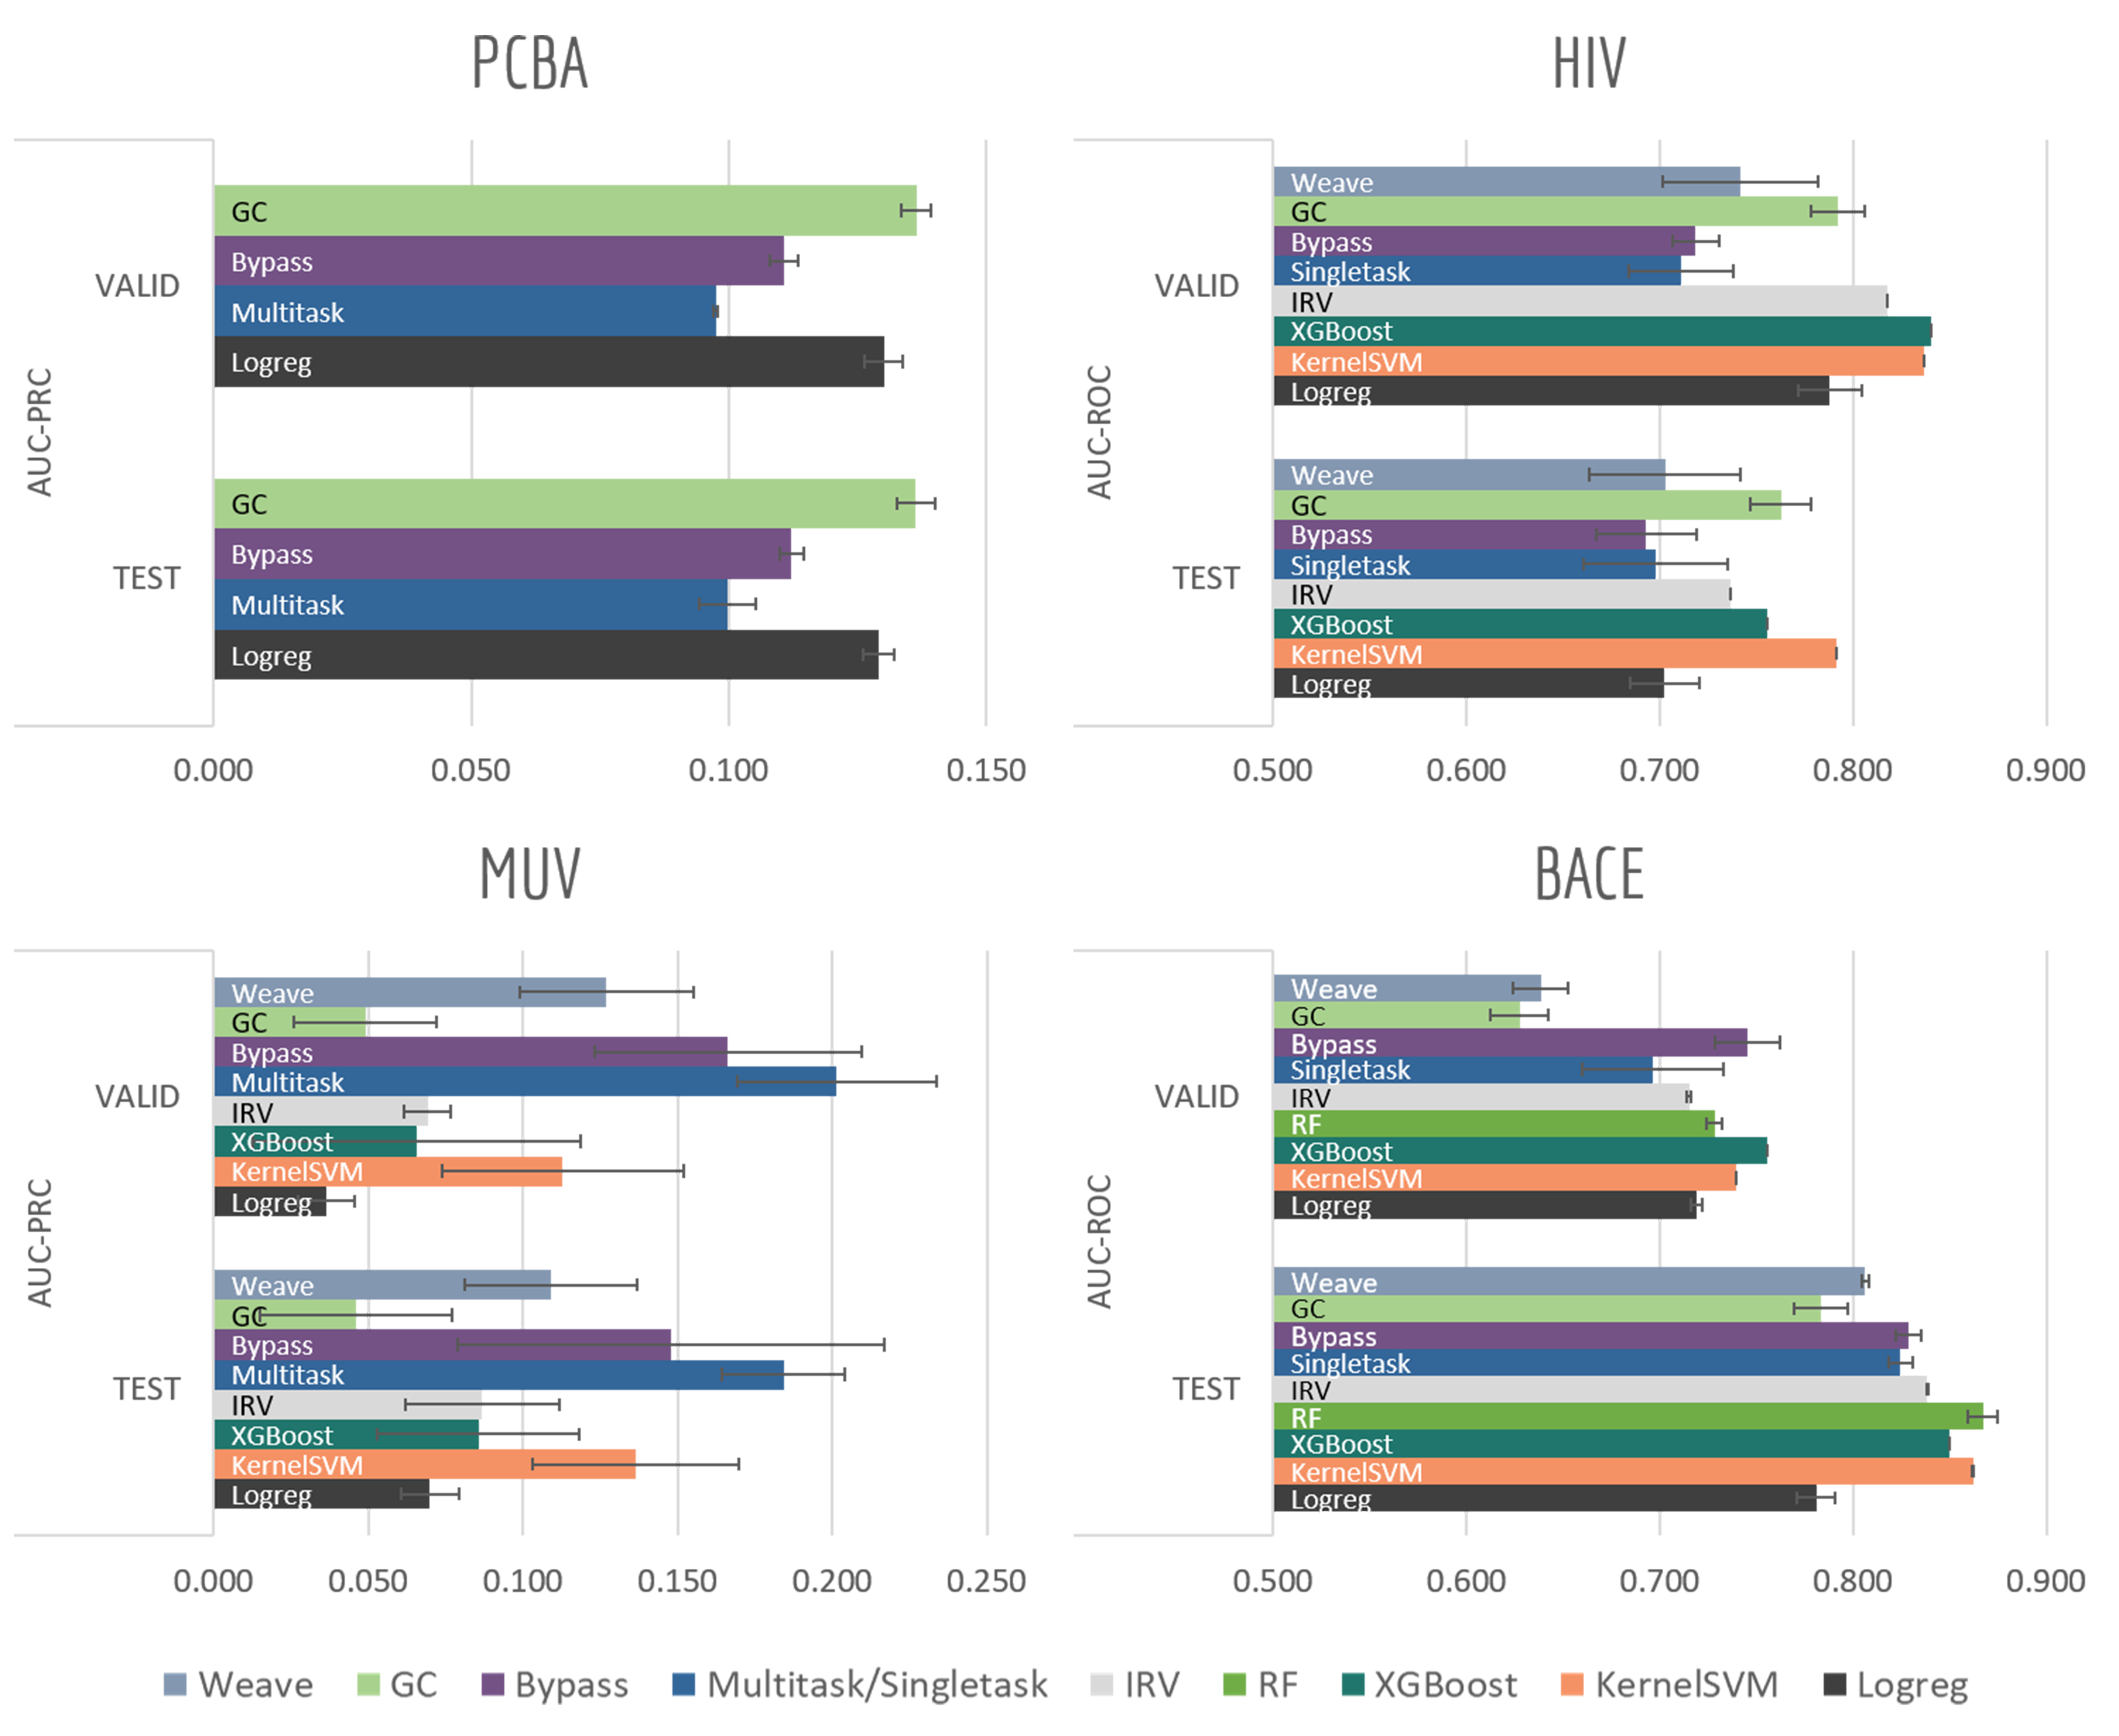
\includegraphics[width=.85\textwidth]{Images/Biophysics.png}
  \caption{Benchmark performances for biophysics tasks: \textbf{PCBA}, 4 models are evaluated by AUC-PRC on random split; \textbf{MUV}, 8 models are evaluated by AUC-PRC on random split; \textbf{HIV}, 8 models are evaluated by AUC-ROC on scaffold split; \textbf{BACE}, 9 models are evaluated by AUC-ROC on scaffold split. For AUC-ROC and AUC-PRC, higher value indicates better performance(to the right).}
  \label{fig:PCBA_HIV_MUV_BACE}
\end{figure*}

\paragraph{Message Passing Neural Networks}

Message passing neural network(MPNN) is a generalized model proposed by Gilmer et al.\cite{MPNN} that targets to formulate a single framework for graph based model. The prediction process is separated into two phases: message passing phase and readout phase. Multiple message passing phases are stacked to extract abstract information of the graph, then the readout phase is responsible for mapping the graph to its properties.

Here we reimplemented the best-performing model in the original article: using an Edge network as message passing function and a set2set model\cite{set2set} as readout function. In message passing phase, an edge-dependent neural network maps all neighbour atoms' feature vectors to updating messages, which are then merged using gated recurrent units. In the final readout phase, feature vectors for all atoms are regarded as a set, then an LSTM using attention mechanism is applied on the set for multiple steps, with its final state used as the output for the molecule.

\subsection{Results and Discussion}

In this section, we discuss the performance of benchmarked models on MoleculeNet datasets. Different models are applied depending on the size, features and task types of the dataset. All graph models use their corresponding featurizations. Non-graph models use ECFP featurizations by default, Coulomb Matrix (CM) and Grid featurizer are also applied for certain datasets.

We run a brief Gaussian process hyperparameter optimization on each combination of dataset and model. Then three independent runs with different random seeds are performed. More detailed description of optimization method and performance tables can be found in supplementary information\dag. Note that all benchmark results presented here are the average of three runs, with standard deviations listed or illustrated as error bars.

We also run a set of experiments focusing on how variable size of training set affect model performances.(Tox21, FreeSolv and QM7) Details will be presented in the following texts.

\subsubsection{Biophysics and Physiology Tasks}

\begin{figure*}[!h]
  \centering
  \includegraphics[width=.85\textwidth]{Images/Physiology.png}
  \caption{Benchmark performances for physiology tasks: \textbf{ToxCast}, 8 models are evaluated by AUC-ROC on random split; \textbf{Tox21}, 9 models are evaluated by AUC-ROC on random split; \textbf{BBBP}, 9 models are evaluated by AUC-ROC on scaffold split; \textbf{SIDER}, 9 models are evaluated by AUC-ROC on random split. For AUC-ROC, higher value indicates better performance(to the right).}
  \label{fig:ToxCast_BBBP_Tox21_SIDER}
\end{figure*}

\begin{figure}[htbp]
  \centering
  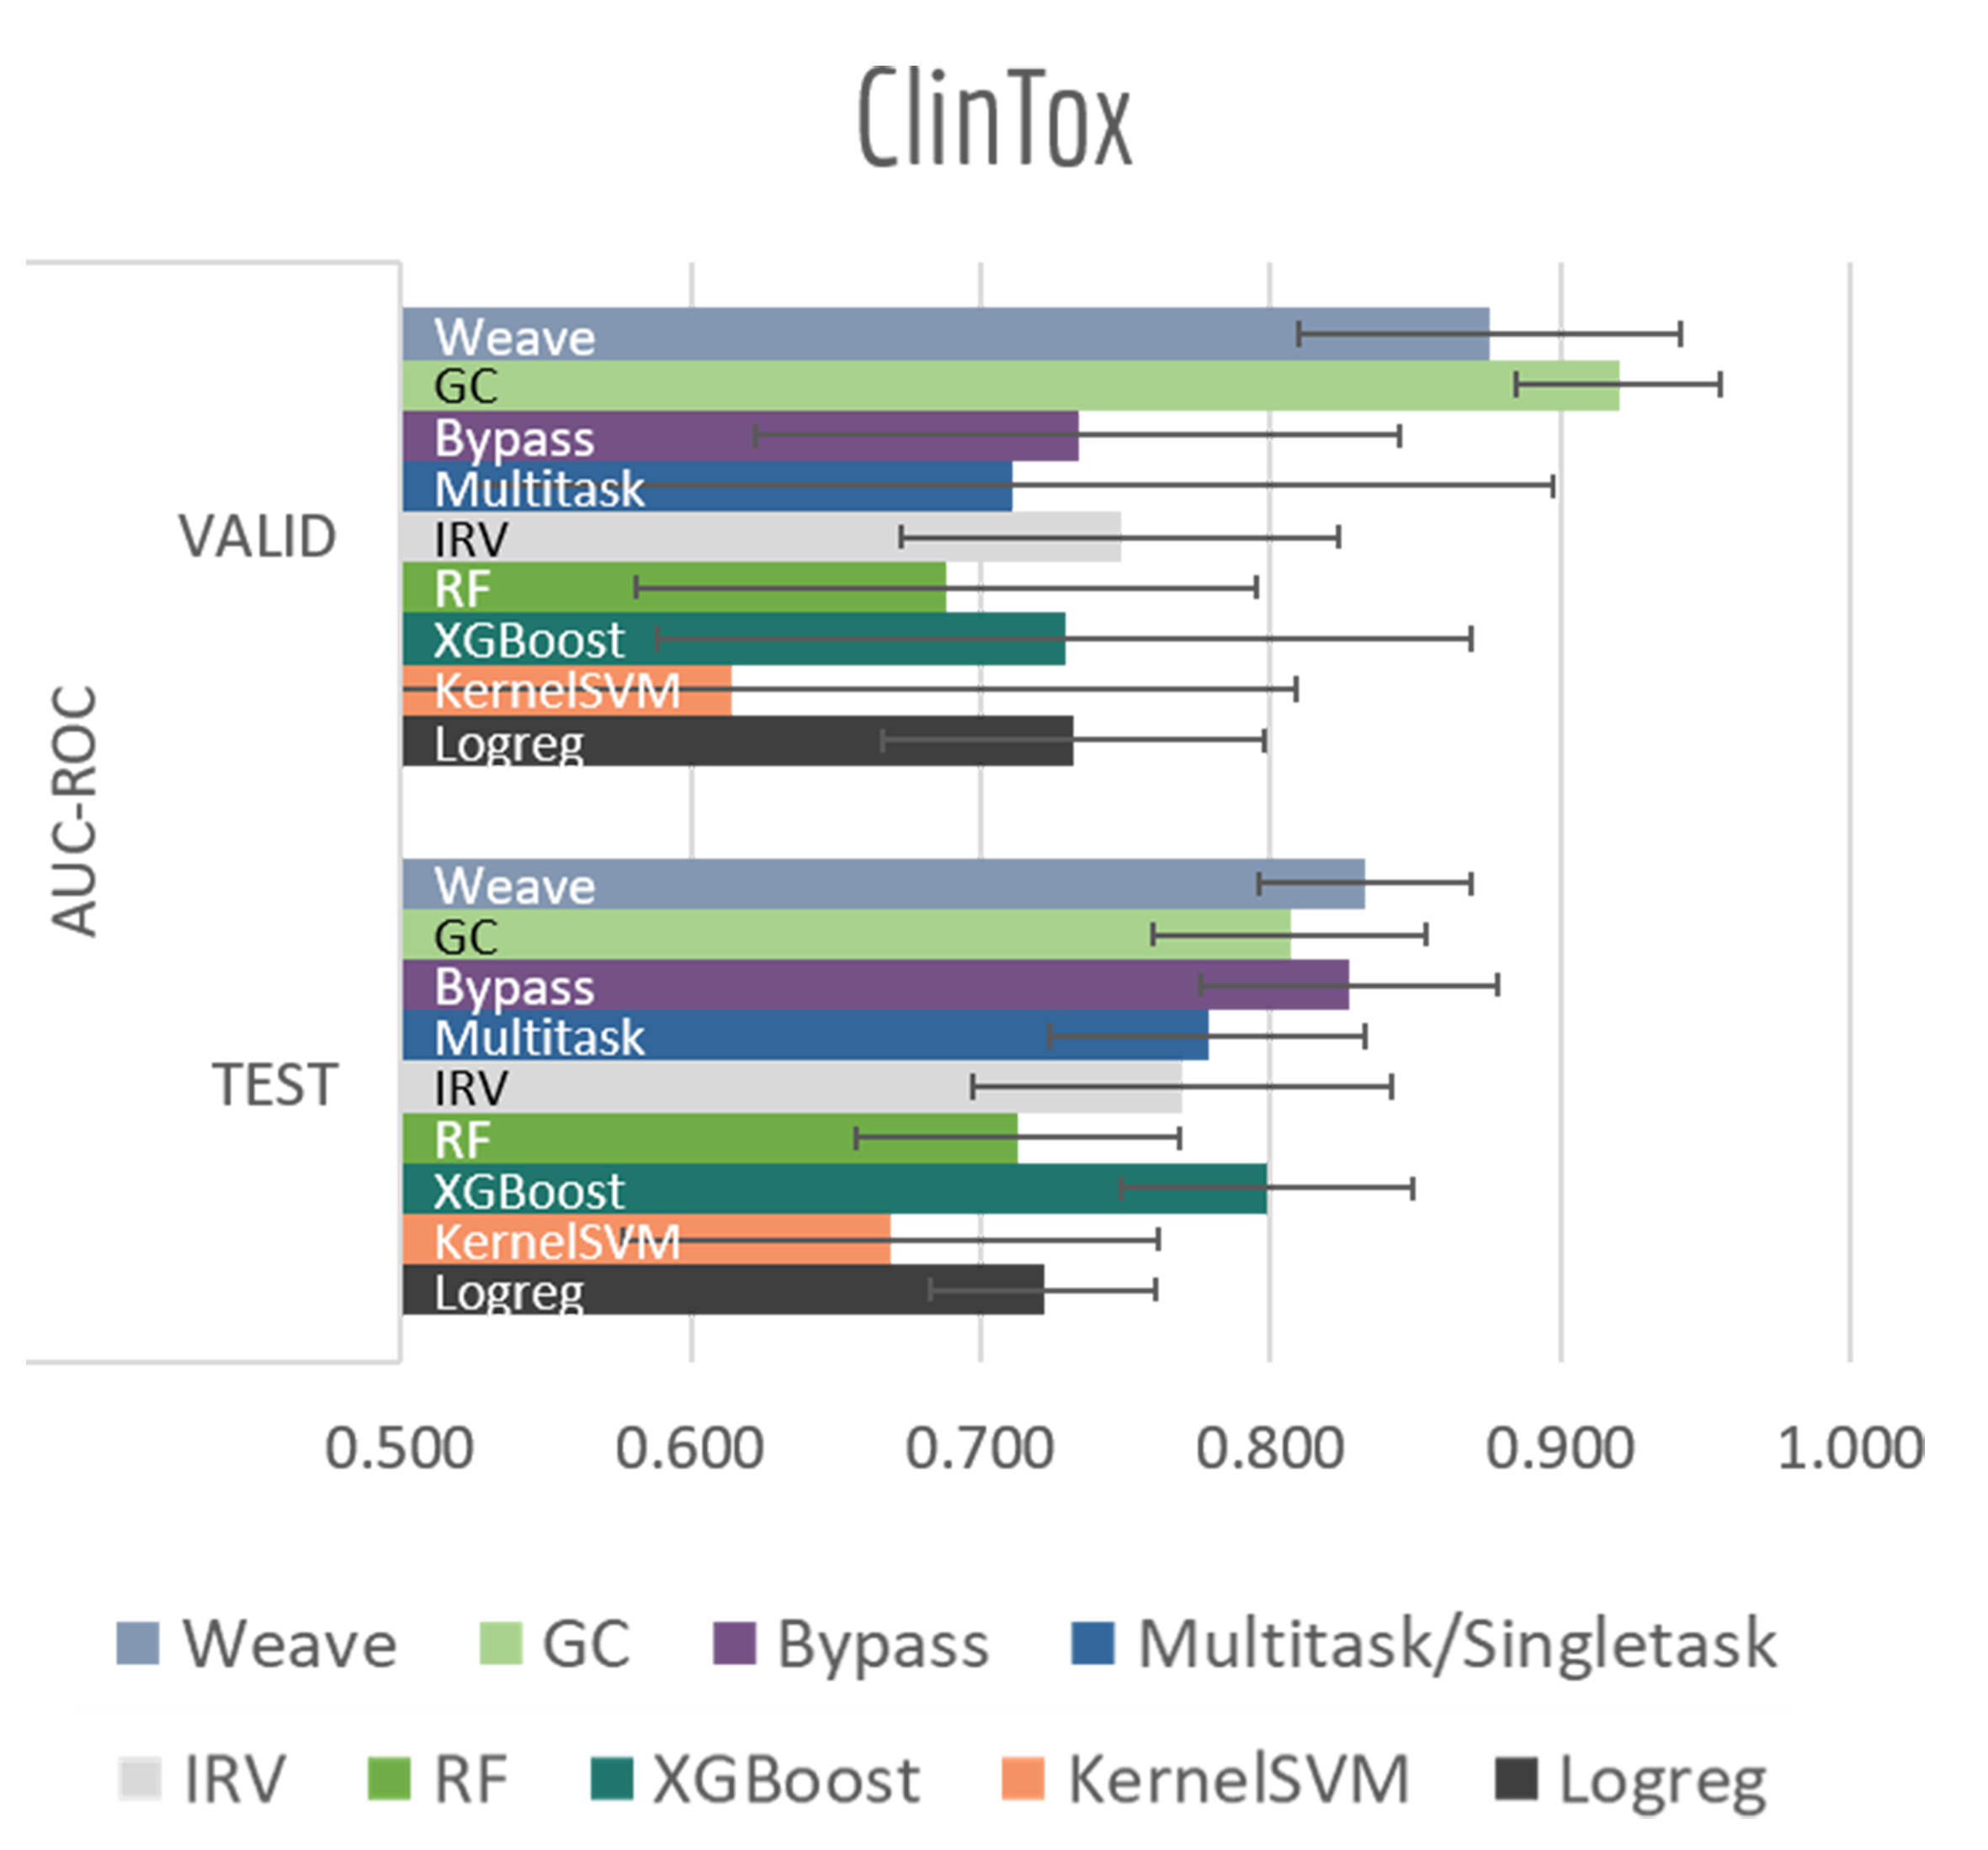
\includegraphics[width=.425\textwidth]{Images/Physiology2.png}
  \caption{Benchmark performances for physiology tasks: \textbf{ClinTox}, 9 models are evaluated by AUC-ROC on random split.}
  \label{fig:ClinTox}
\end{figure}

Tables~\ref{tab:PCBA_MUV_HIV_BACE}, \ref{tab:BBBP_Tox21_ToxCast_SIDER} and Figures~\ref{fig:PCBA_HIV_MUV_BACE}, \ref{fig:ToxCast_BBBP_Tox21_SIDER}, \ref{fig:ClinTox} report AUC-ROC or AUC-PRC results of $4$ to $9$ different models on biophysics datasets (PCBA, MUV, HIV, BACE) and physiology datasets (BBBP, Tox21, Toxcast, SIDER, ClinTox). Some models were too computationally expensive to be run on the larger datasets. All of these datasets contain only classification tasks. 

Most models have train scores (listed in Tables~\ref{tab:PCBA_MUV_HIV_BACE}, \ref{tab:BBBP_Tox21_ToxCast_SIDER}) higher than validation/test scores, indicating that overfitting is a general issue. Singletask logistic regression exhibits the largest gaps between train scores and validation/test scores, while models incorporating multitask structure generally show less overfit, suggesting that multitask training has a regularizing effect. Most physiological and biophysical datasets in MoleculeNet have only a low volume of data for each task. Multitask algorithms combine different tasks, resulting in a larger pool of data for model training. In particular, multitask training can, to some extent, compensate for the limited data amount available for each individual task.

Graph convolutional models and weave models, each based on an adaptive method of featurization\cite{graphconv_feat, kearnes2016graphconv}, show strong validation/test results on larger datasets, along with less overfit. Similar results are reported in previous graph-based algorithms \cite{kearnes2016graphconv, graphconv_feat, MPNN, schutt2016quantum, lusci2013deep}, showing that learnable featurizations can provide a large boost compared with conventional featurizations.

For smaller singletask datasets (less than 3000 samples), differences between models are less clear. Kernel SVM and ensemble tree methods (gradient boosting and random forests) are more robust under data scarcity, while they generally need longer running time (see Table~\ref{tab:running_time}). Worse performances of graph-based models are within expectation as complex models generally require more training data.

Bypass networks show higher train scores and equal or higher validation/test scores compared with vanilla multitask networks, suggesting that the bypass structure does add robustness. IRV models achieve performance broadly comparable with multitask networks. However, the quadratic nearest neighbor search makes the IRV models slower to train than the multitask networks (see Table~\ref{tab:running_time}).

Three datasets (HIV, BACE, BBBP) in these two categories are evaluated under scaffold splitting. As compounds are divided by their molecular scaffolds, increasing differences between train, validation and test performances are observed. Scaffold splits provide a stronger test of a given model's generalizability compared with random splitting. Two datasets (PCBA, MUV) are evaluated by AUC-PRC, which is more practically useful under high class imbalance as discussed above. Graph convolutional model performs the best on PCBA (positive rate $1.40\%$), while results on MUV (positive rate $0.20\%$) are much less stable, which is most likely due to its extreme low amount of positive samples. Under such high imbalance, graph-based models are still not robust enough in controlling false positives.

\begin{figure}[!h]
  \centering
  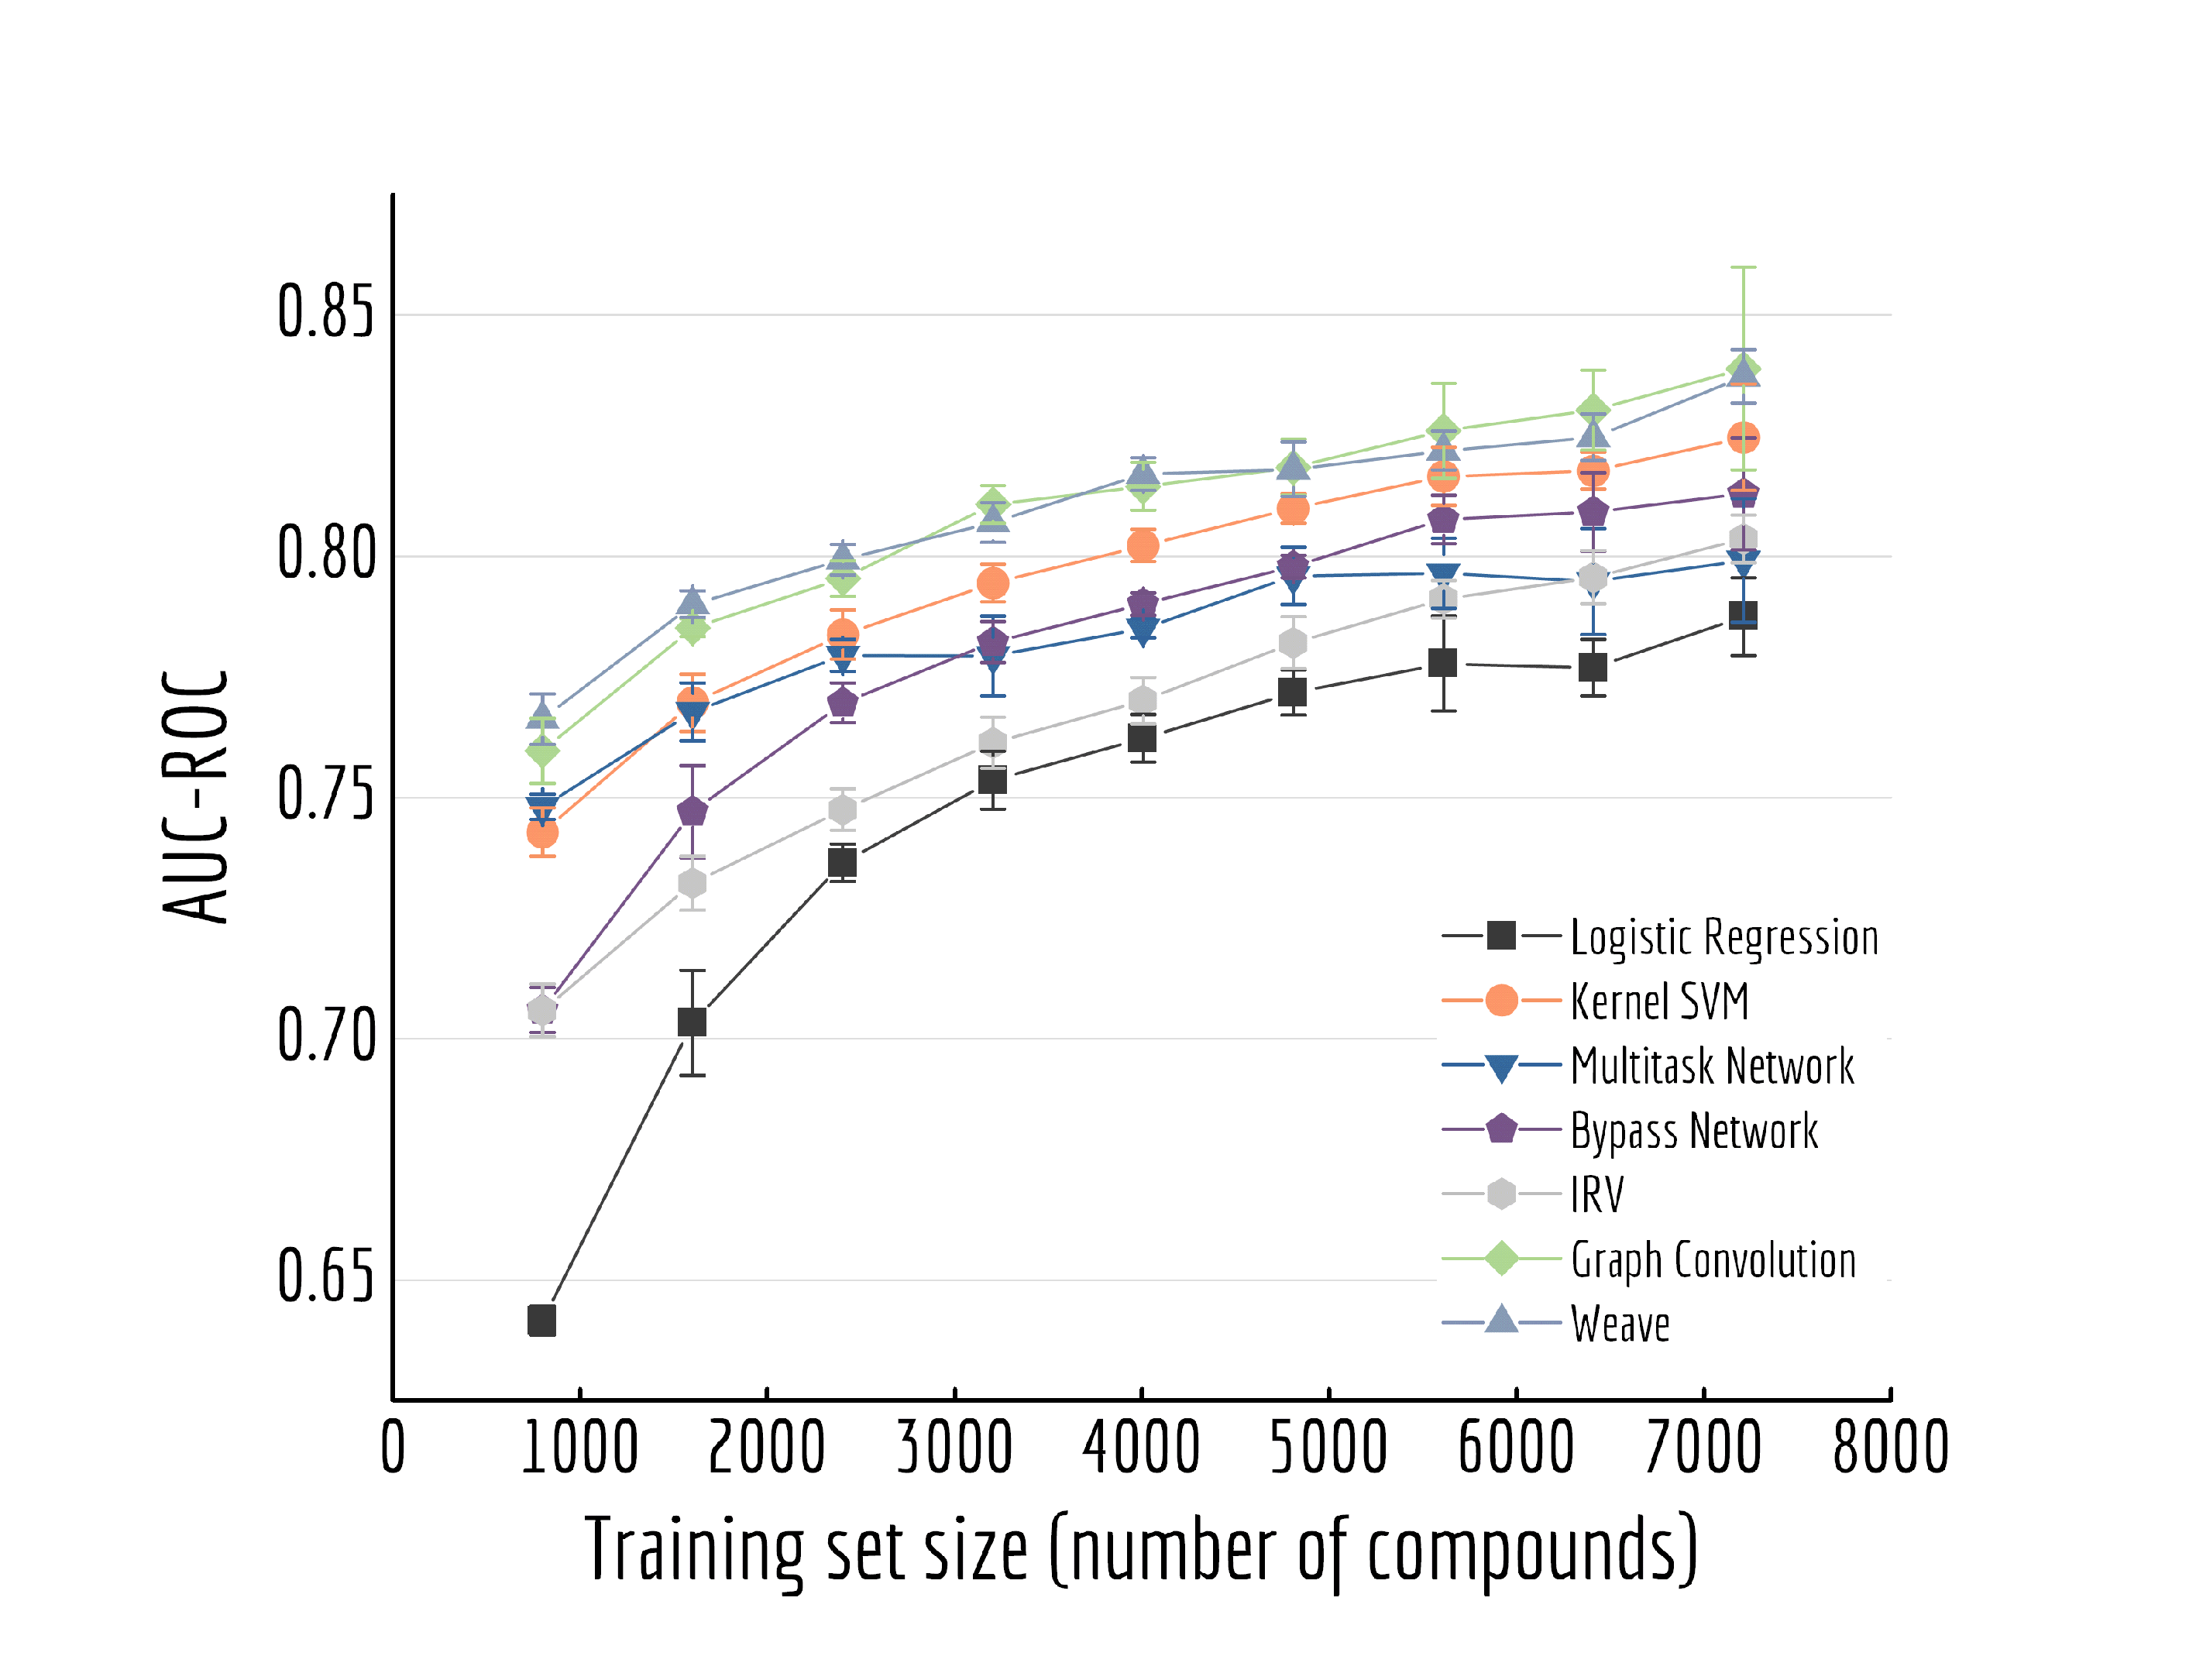
\includegraphics[width=.45\textwidth]{Images/Tox21_variable.png}
  \caption{Out-of-sample performances with different training set sizes on Tox21. Each datapoint is the average of 5 independent runs, with standard deviations shown as error bars.}
  \label{fig:Tox21_variable}
\end{figure}

Here we performed a more detailed experiment to illustrate how model performances change with increasing training samples. We trained multiple models on Tox21 with training sets of different size($10\%$ to $90\%$ of the whole dataset) Figure~\ref{fig:Tox21_variable} displayed mean out-of-sample performances (and standard deviations) of five independent runs. A clear increase on performance is observed for each model, and graph-based models (Graph convolutional model and weave model) always stay on top of the lines. By drawing a horizontal line at around 0.80, we can see graph-based models achieve the similar level of accuracy with multitask networks by using only one-third of the training samples($30\%$ versus $90\%$).

\begin{figure}[!h]
  \centering
  \includegraphics[width=0.425\textwidth]{Images/PDBbind.png}
  \caption{Benchmark performances of \textbf{PDBbind}: 5 models are evaluated by RMSE on the three subsets: core, refined and full. Time split is applied to all three subsets. Noe that for RMSE, lower value indicates better performance(to the right).}
  \label{fig:PDBbind}
\end{figure}

\begin{figure}[!h]
  \centering
  \includegraphics[width=.425\textwidth]{Images/PhysicalChemistryTasks.png}
  \caption{Benchmark performances for physical chemistry tasks: \textbf{ESOL}, 8 models are evaluated by RMSE on random split; \textbf{FreeSolv}, 8 models are evaluated by RMSE on random split; \textbf{Lipophilicity}, 8 models are evaluated by RMSE on random split. Note that for RMSE, lower value indicates better performance(to the right).}
  \label{fig:ESOL_FreeSolv_Lipo}
\end{figure}

\subsubsection{Biophysics Task - PDBbind}

The PDBBind dataset maps distinct ligand-protein structures to their binding affinities. As discussed in the datasets section, we created grid featurizer to harness the joint ligand-protein structural information in PDBBind to build a model that predicts the experimental $K_i$ of binding. We applied time splitting to all three subsets: core, refined, and full subsets of PDBbind(Core contains roughly 200 structures, refined 4000, and full 15000. The smaller datasets are cleaned more thoroughly than larger datasets.), with all results displayed in Table~\ref{tab:PDBbind} and Figure~\ref{fig:PDBbind}. Clearly as dataset size increased, we can see a significant boost on validation/test set performances. At the same time, for the two larger subsets: refined and full, switching from pure ligand-based ECFP to grid featurizer do increase the performances by a small margin in both Singletask networks and random forests. While for core subset, all models are showing relatively high errors and two featurizations do not show clear differences, which is within expectation as sample amount in core subset is too small to support a stable model performance. Note that models on the full set aren't significantly superior to models with less data; this effect may be due to the additional data being less clean.

Note that all models display heavy overfitting. Additional clean data may be required to create more accurate models for protein-ligand binding.

\subsubsection{Physical Chemistry Tasks}

Solubility, solvation free energy and lipophilicity are basic physical chemistry properties important for understanding how molecules interact with solvents. Figure~\ref{fig:ESOL_FreeSolv_Lipo} and Table~\ref{tab:ESOL_FreeSolv_Lipo} presented performances on predicting these properties. 

Graph-based methods: graph convolutional model, DAG, MPNN and weave model all exhibit significant boosts over vanilla singletask network, indicating the advantages of learnable featurizations. Differences between graph-based methods are rather minor and task-specific. The best-performing models in this category can already reach the accuracy level of \textit{ab-initio} predictions(+/- 0.5 for ESOL, +/- 1.5 kcal/mol for FreeSolv).

We performed a more detailed comparison between data-driven methods and \textit{ab-initio} calculations on FreeSolv. Hydration free energy has been widely used as a test of computational chemistry methods. With free energy values ranging from $-25.5$ to $3.4\mbox{kcal/mol}$ in the FreeSolv dataset, RMSE for calculated results reach up to $1.5\mbox{kcal/mol}$.\cite{SAMPL4} On the other hand, though machine learning methods typically need large amounts of training data to acquire predictive power, they can achieve higher accuracies given enough data. We investigate how the performance of machine learning methods on FreeSolv changes with the volume of training data. In particular, we want to know the amount of data required for machine learning to achieve accuracy similar to that of physically inspired algorithms.

\begin{figure}[htbp]
  \centering
  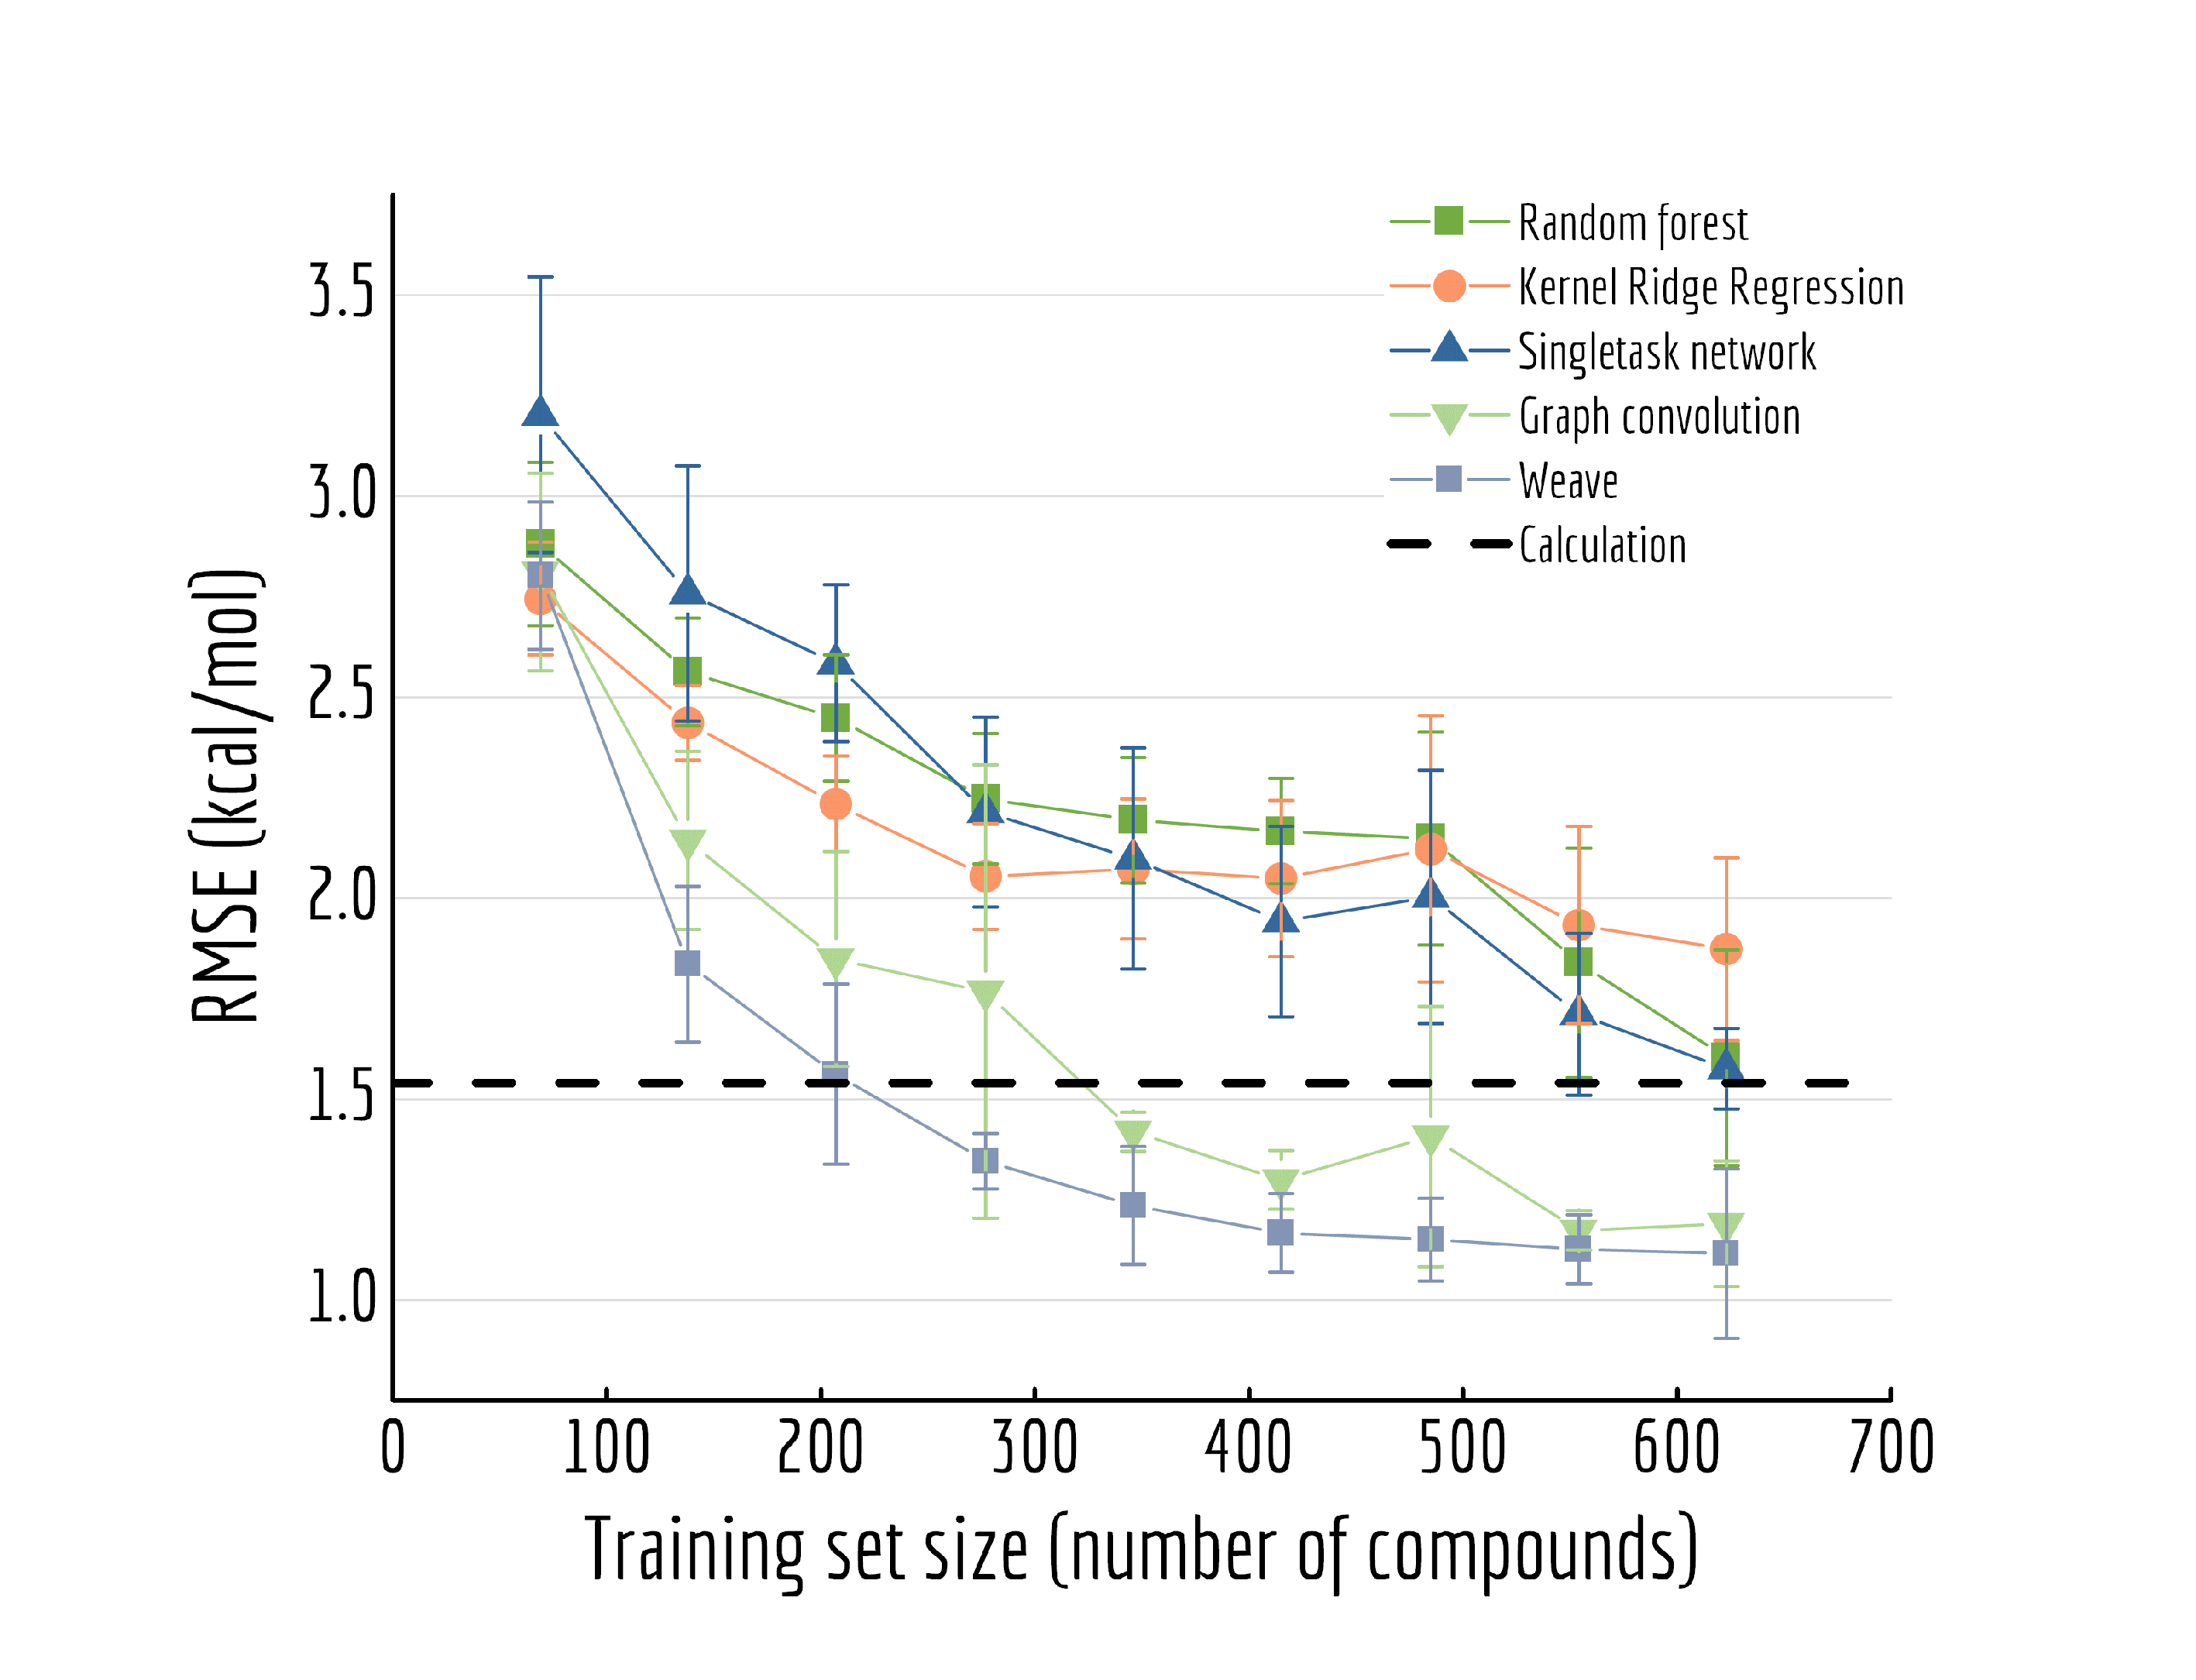
\includegraphics[width=.45\textwidth]{Images/FreeSolv_variable.png}
  \caption{Out-of-sample performances with different training set sizes on FreeSolv. Each datapoint is the average of 5 independent runs, with standard deviations shown as error bars.}
  \label{fig:FreeSolv_variable}
\end{figure}

For Figure~\ref{fig:FreeSolv_variable}, we similarly generated a series of models with different training set volumes and calculated their out-of-sample RMSE. Each data point displayed is the average of 5 independent runs, with standard deviations displayed as error bars. Both graph convolutional model and weave model are capable of achieving better performances with enough training samples ($30\%$ and $50\%$ of the data respectively). Given the size of FreeSolv dataset is only around 600 compounds, a weave model can reach state-of-the-art free energy calculation performances by training on merely 200 samples. On the other hand, comparing with singletask network's performance, weave model achieved the same level of accuracy with only one-third of the training samples.

\subsubsection{Quantum Mechanics Tasks}

\begin{figure}[htbp]
  \centering
  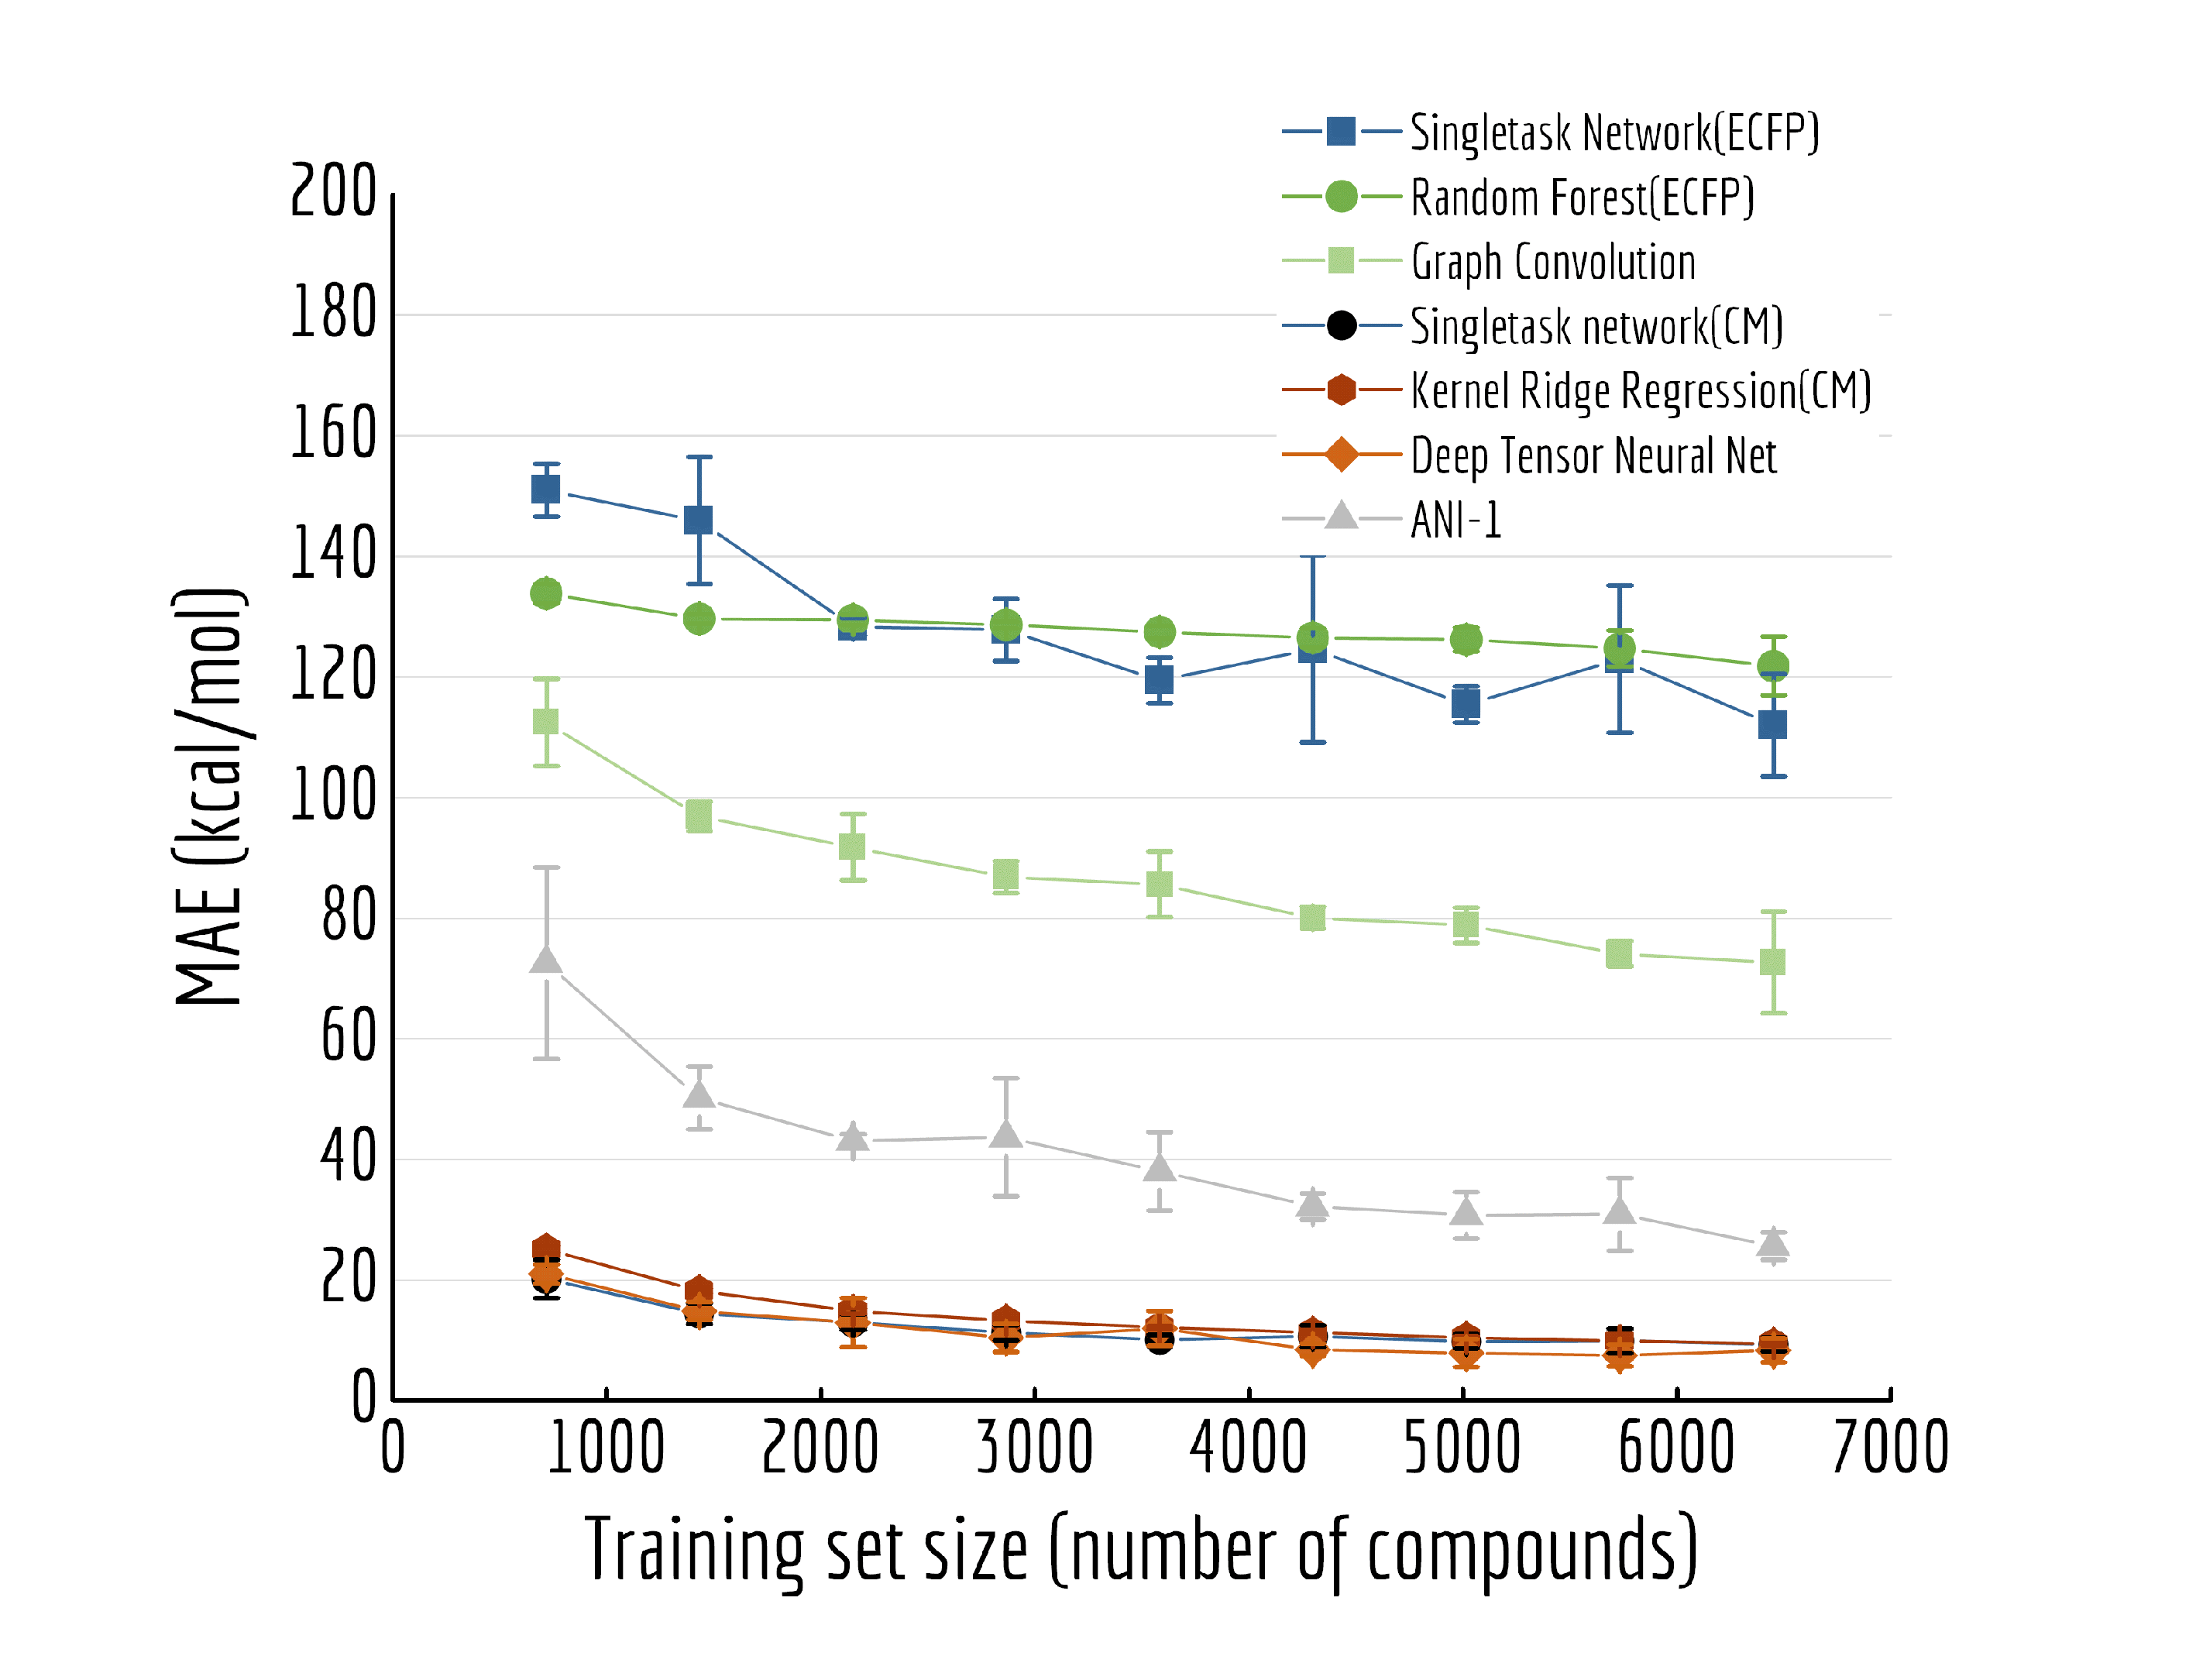
\includegraphics[width=.45\textwidth]{Images/QM7_variable.png}
  \caption{Out-of-sample performances with different training set sizes on QM7. Each datapoint is the average of 5 independent runs, with standard deviations shown as error bars.}
  \label{fig:QM7_variable}
\end{figure}

\begin{figure}[htbp]
  \centering
  \includegraphics[width=.425\textwidth]{Images/QM.png}
  \caption{Benchmark performances for quantum mechanics tasks: \textbf{QM7}, 8 models are evaluated by MAE on stratified split; \textbf{QM7b}, 3 models (QM7b only provides 3D coordinates) are evaluated by MAE on random split; \textbf{QM8}, 7 models are evaluated by MAE on random split; \textbf{QM9}, 5 models are evaluated by MAE on random split. Note that for MAE, lower value indicates better performance(to the right)}
  \label{fig:QM}
\end{figure}

The QM datasets (QM7, QM7b, QM8, QM9) represent another distinct category of properties that are typically calculated through solving Schr\"odinger's equation (approximately using techniques such as DFT). As most conventional methods are slower than data-driven methods by orders of magnitude, we hope to learn effective approximators by training on existing datasets.

Table~\ref{tab:QM7_QM7b_QM8_QM9} and Figure~\ref{fig:QM} display the performances in mean absolute error of multiple methods. Table~\ref{tab:QM7b}, \ref{tab:QM8} and \ref{tab:QM9} show detailed performances for each task.(Due to difference in range of labels, mean performances of QM7b and QM9 are more skewed) Unsurprisingly, significant boosts on performances and less overfitting are observed for models incorporating distance information (multitask networks and KRR with Coulomb Matrix featurization, DTNN, MPNN). In particular, KRR and multitask networks(CM) outperform their corresponding baseline models in QM7 and QM9 by a large margin, while DTNN and MPNN display less error comparing with graph convolutional models as well. At the same time, DTNN and MPNN gains better performances than multitask networks and KRR (CM) on most tasks. Table~\ref{tab:QM7b} shows that DTNN outperforms KRR(CM) on 12/14 tasks in QM7b(Though the mean error shows the opposite result due to averaging errors on different magnitudes). In total, DTNN and MPNN covers the best-performing models on 28/39 of all tasks in this category, again reflecting the superiority of learnable featurization.

Another variable trainging size experiment is performed on QM7: predicting atomization energy. All mean absolute error performances are displayed in Figure~\ref{fig:QM7_variable}. Clearly incorporation of spatial position creates the huge gap between models, DTNN and multitask networks(CM) reach similar level of accuracy as reported in previous work on this dataset. (There is still a gap between the MoleculeNet implementation and best reported numbers from previous work\cite{GDB7_dataset_arxiv, schutt2016quantum}, which would likely be closed by training models longer). ANI-1 is also reported to achieve comparable performances on similar task in the previous work\cite{ANI-1} with a much larger dataset. Apparently its worse performance is restricted by training set size, as the MAE is keep decreasing with more training samples.

For QM series, proper choice of featurization appears critical. As mentioned previously, ECFP only consider graph substructures, while Coulomb Matrix and graph featurizations used by DTNN and MPNN are explicitly calculated on charges and physical distances, which are exactly the required input for  solving Schr\"odinger's equation. 



\subsection{Conclusions}

\begin{table*}[htbp]
    \caption{Summary of performances(test subset): conventional methods versus graph-based methods. Graph-based models outperform conventional methods on 11/17 datasets.}
    \centering
    \label{tab:conventional_versus_graph}
    \begin{threeparttable}[b]
    \begin{tabular*}{\textwidth}{@{\extracolsep{\fill}}lllll}
    \hline
    \multirow{2}{*}{\textbf{Category}} & \multirow{2}{*}{\textbf{Dataset}} & \multirow{2}{*}{\textbf{Metric}} & \textbf{Best performances - } & \textbf{Best performances - }\\
    & & & \textbf{conventional methods} & \textbf{graph-based methods} \\
    \hline
    \multirow{4}{*}{Quantum Mechanics} & QM7 & MAE & KRR(CM): 10.22 & \textbf{DTNN: 8.75} \\\cline{2-5}
    & QM7b & MAE & KRR(CM): 1.05 & \textbf{DTNN: 1.77*} \\\cline{2-5}
    & QM8 & MAE & Multitask: 0.0150 & \textbf{MPNN: 0.0143} \\\cline{2-5}
    & QM9 & MAE & Multitask(CM): 4.35 & \textbf{DTNN: 2.35} \\\cline{2-5}
    \hline
    \multirow{3}{*}{Physical Chemistry} & ESOL & RMSE & XGBoost: 0.99 & \textbf{MPNN: 0.58} \\\cline{2-5}
    & FreeSolv & RMSE & XGBoost: 1.74 & \textbf{MPNN: 1.15} \\\cline{2-5}
    & Lipophilicity & RMSE & XGBoost: 0.799 & \textbf{GC: 0.655} \\
    \hline
    \multirow{5}{*}{Biophysics} & PCBA & AUC-PRC & Logreg: 0.129 & \textbf{GC: 0.136} \\\cline{2-5}
    & MUV & AUC-PRC & \textbf{Multitask: 0.184} & Weave: 0.109 \\\cline{2-5}
    & HIV & AUC-ROC & \textbf{KernelSVM: 0.792} & GC: 0.763 \\\cline{2-5}
    & BACE & AUC-ROC & \textbf{RF: 0.867} & Weave: 0.806 \\\cline{2-5}
    & PDBbind(full) & RMSE & \textbf{RF(grid): 1.25} & GC: 1.44 \\
    \hline
    \multirow{5}{*}{Physiology} & BBBP & AUC-ROC & \textbf{KernelSVM: 0.729} & GC: 0.690 \\\cline{2-5}
    & Tox21 & AUC-ROC & KernelSVM: 0.822 & \textbf{GC: 0.829} \\\cline{2-5}
    & ToxCast & AUC-ROC & Multitask: 0.702 & \textbf{Weave: 0.742} \\\cline{2-5}
    & SIDER & AUC-ROC & \textbf{RF: 0.684} & GC: 0.638 \\\cline{2-5}
    & ClinTox & AUC-ROC& Bypass: 0.827 & \textbf{Weave: 0.832} \\
    \hline
    \end{tabular*}    
    \begin{tablenotes}
        \item * As discussed in section 4.4, DTNN outperforms KRR(CM) on 14/16 tasks in QM7b while the mean-MAE is skewed due to different magnitudes of labels.
    \end{tablenotes}
    \end{threeparttable}
\end{table*}

This work introduces MoleculeNet, a benchmark for molecular machine learning. We gathered data for a wide range of molecular properties: 17 dataset collections including over 800 different tasks on 700,000 compounds. Tasks are categorized into 4 levels as illustrated in Figure~\ref{fig:dataset_composition}: (i) quantum mechanical characters; (ii) physical chemistry properties; (iii) biophysical affinity and activity with bio-macromolecules; (iv) macroscopic physiological effects on human body. 

MoleculeNet contributes a data-loading framework, featurization methods, data splitting methods, and learning models to the open source DeepChem package (Figure~\ref{fig:benchmark_example}). By adding interchangeable featurizations, splits and learning models into the DeepChem framework, we can apply these primitives to the wide range of datasets in MoleculeNet. 

Broadly, our results show that graph-based models (graph convolutional models, weave models and DTNN) outperform other methods by comfortable margins on most datasets(11/17, best performances comparison in Table~\ref{tab:conventional_versus_graph}), revealing a clear advantage of learnable featurizations. However, this effect has some caveats: Graph-based methods are not robust enough on complex tasks under data scarcity; on heavily imbalanced classification datasets, conventional methods such as kernel SVM outperform learnable featurizations with respect to recall of positives. Furthermore, for the PDBBind and quantum mechanics datasets, the use of appropriate featurizations which contains pertinent information is very significant. Comparing fully connected neural networks, random forests, and other comparatively simple algorithms, we claim that the PDBbind and QM7 results emphasize the necessity of using specialized features for different tasks. DTNN and MPNN which use distance information perform better on QM datasets than simple graph convolutions. While out of the scope of this paper, we note similarly that customized deep learning algorithms \cite{AtomNet} could in principle supplant the need for hand-derived, specialized features in such biophysical settings. On the FreeSolv dataset, comparison between conventional \textit{ab-initio} calculations and graph-based models for the prediction of solvation energies shows that data-driven methods can outperform physical algorithms with moderate amounts of data. These results suggest that data-driven physical chemistry will become increasingly important as methods mature. Results for biophysical and physiological datasets are currently weaker than for other datasets, suggesting that better featurizations or more data may be required for data-driven physiology to become broadly useful.

%ENF: the conclusions here about PDBBind and QM7/7b are in part correct, but we may want to nuance it. *Given Fully connected neural networks, RFs, and other relatively simple ML techniques that do not have the capacity to learn higher-order features, the physical elements of featurization is more important than the ML algorithm. However, AtomWise's AtomNet and Gomes et al Atomic ConvNet paper do and will show that this is not true given sufficiently fancy DNNs, right?

By providing a uniform platform for comparison and evaluation, we hope MoleculeNet will facilitate the development of new methods for both chemistry and machine learning. In future work, we hope to extend MoleculeNet to cover a broader range of molecular properties than considered here. For example, 3D protein structure prediction, or DNA topological modeling would benefit from the presence of strong benchmarks to encourage algorithmic development. We hope that the open-source design of MoleculeNet will encourage researchers to contribute implementations of other novel algorithms to the benchmark suite. In time, we hope to see MoleculeNet grow into a comprehensive resource for the molecular machine learning community.

\subsection{Acknowledgements}
We would like to thank the Stanford Computing Resources for providing us with access to the Sherlock and Xstream GPU nodes. Thanks to Steven Kearnes and Patrick Riley for early discussions about the MoleculeNet concept. Thanks to Aarthi Ramsundar for help with diagram construction.

Thanks to Zheng Xu for feedback on the MoleculeNet API. Thanks to Patrick Hop for contribution of the Lipophilicity dataset to MoleculeNet. Thanks to Anthony Gitter and Johnny Israeli for suggesting the addition of AuPRC for imbalanced datasets. Thanks to Keri McKiernan for composing the tutorial of preparing datasets.

The Pande Group is broadly supported by grants from the NIH (R01 GM062868 and U19 AI109662) as well as gift funds and contributions from Folding@home donors. 


We acknowledge the generous support of Dr. Anders G. Fr{\o}seth and Mr. Christian Sundt for our work on machine learning.

B.R. was supported by the Fannie and John Hertz Foundation.

%%%END OF MAIN TEXT%%%

%The \balance command can be used to balance the columns on the final page if desired. It should be placed anywhere within the first column of the last page.

%\balance

%If notes are included in your references you can change the title from 'References' to 'Notes and references' using the following command:
%\renewcommand\refname{Notes and references}

%%%REFERENCES%%%
%\bibliography{rsc} %You need to replace "rsc" on this line with the name of your .bib file
%\bibliographystyle{rsc} %the RSC's .bst file

%\end{document}

\clearpage
\section{Low Data Drug Discovery with One-Shot Learning}

\begin{abstract}
Recent advances in machine learning have made significant contributions to drug discovery. Deep neural networks in particular have been demonstrated to provide significant boosts in predictive power when inferring the properties and activities of small-molecule compounds \cite{ma2015deep}. However, the applicability of these techniques has been limited by the requirement for large amounts of training data. In this work, we demonstrate how one-shot learning can be used to significantly lower the amounts of data required to make meaningful predictions in drug discovery applications. We introduce a new architecture, the iterative refinement LSTM, that, when combined with graph convolutional neural networks, significantly improves learning of meaningful distance metrics over small-molecules. We open source all models introduced in this work as part of DeepChem, an open-source framework for deep-learning in drug discovery
\cite{ram2016}.
\end{abstract}

\subsection{Introduction}
The lead optimization step of drug discovery is fundamentally a low-data problem. When biological studies yield evidence that a particular molecule can modulate essential pathways to achieve therapeutic activity, the discovered molecule often fails as a potential drug for a number of reasons including toxicity, low activity, and low solubility \cite{waring2015analysis}. The central problem of small-molecule based drug-discovery is to optimize the candidate molecule by finding analogue molecules with increased pharmaceutical activity and reduced risks to the patient. Yet, with only a small amount of biological data available on the candidate and related molecules, it is challenging to form accurate predictions for novel compounds.

In the last few years, the field of machine-learning has produced several pivotal advances that address complex problems. Deep neural networks have solved challenging problems in visual perception \cite{ILSVRC15}, speech-recognition \cite{deng2013new}, language translation \cite{wu2016google}, and game-playing \cite{silver2016mastering}. These techniques leverage the use of multilayer neural network architectures as powerful and flexible function approximators. This capability of deep neural networks is underpinned by their ability to learn sophisticated representations of their input given large amounts of data.

These advances in deep-learning have inspired novel approaches for better understanding chemistry. For example, in 2012, Merck sponsored a Kaggle competition for improving the accuracy of molecular property prediction. The winning team used multitask deep networks and achieved a 15\% improvement in relative accuracy over a random forest baseline \cite{dahl2012deep}. Following this work, many groups demonstrated that massively multitask networks can provide significant boosts in the predictive power of deep-learning models for property prediction \cite{ramsundar2015massively, unterthiner2014deep}. In parallel, other groups developed sophisticated deep-architectures for processing and extracting features from molecular structures \cite{lusci2013deep}. Graph-convolutional architectures \cite{duvenaud2015convolutional, kearnes2016molecular} in particular process small-molecules as undirected graphs and build up features using learnable convolution layers. In contrast to older small-molecule featurizing algorithms, such as circular fingerprints\cite{rogers2010extended}, these new graph convolutional feature extracting architectures are learnable, meaning they can be modified to improve performance. 

The practical effect of these innovations in drug discovery has been limited as most of the aforementioned deep-learning frameworks require large-amounts of data. For example, massively multitask networks have so far been trained with millions of datapoints \cite{ramsundar2015massively}. This is in stark contrast to the state of current drug discovery pipelines, which often struggle to characterize even a few dozen compounds. Recent work has demonstrated that standard machine-learning techniques such as random forests and simple deep-networks are capable of learning meaningful chemical information from only a few hundred compounds \cite{subramanian2016computational}, but even a hundred compounds is often too resource intensive for standard drug discovery campaigns. 

Other recent advances in machine learning have demonstrated that in some circumstances, non-trivial predictors may be learned from only a few datapoints \cite{lake2015human, santoro2016one, vinyals2016matching}. These methods work by using related data to learn a meaningful distance metric over the space of possible inputs. This sophisticated metric is used to compare new datapoints to the limited available data and subsequently predict properties of these new datapoints. More broadly, these techniques are known as "one-shot learning" methods. For example, matching-networks \cite{vinyals2016matching}, learn a distance-metric upon images which they use to achieve impressive near-human accuracies on the one-shot character-recognition Omniglot dataset \cite{lake2015human}.

In this work, we mathematically adapt the standard one-shot learning paradigm to the the drug discovery problem. Standard one-shot learning focuses on recognizing new-classes (say recognizing a giraffe given only one example). In drug-discovery, the challenge is rather to predict the behavior of a molecule in a new experimental system.

We introduce a new deep-learning architecture, the iterative refinement LSTM, a modification of the matching-networks architecture and the the residual convolutional network \cite{he2016identity}. This architecture allows for the learning of sophisticated metrics which can trade information between evidence and query molecules. We demonstrate that this architecture offers significant boosts in predictive power for a variety of problems meaningful for low-data drug discovery.

Furthermore, we take a strong open-source approach in this work. Every primitive introduced in this paper is open-sourced as part of the DeepChem \cite{ram2016} library for open-source drug discovery. In particular we provide high-quality Tensorflow \cite{abadi2016tensorflow} implementations of graph-convolutional primitives along with implementations of our one-shot learning models. The scripts used to generate all numbers in this paper are similarly open sourced, along with all datasets. Interested parties can reproduce all results claimed in this work with relative ease.

%\subsection{Related Work}
%Matching Networks Paper. Massively Multitask Networks for Drug %Discovery. Merck Deep Learning Papers. Graph convolutions. Google Graph %Convolutions. 

\subsection{Results and Discussion}

This paper introduces the task of low data learning for drug discovery, and provides an architecture for learning such models. We demonstrate that this architecture can provide strong boosts over simpler methods for low-data learning. On the Tox21 and SIDER collections, one-shot learning methods strongly dominate simpler machine learning baselines. This result is particularly interesting for the SIDER collection, since this dataset consists of very high-level phenotypic side-effect observations. Given the amount of uncertainty in these predictions, the fact that one-shot learning is able to do well is a strong indication that these methods could offer strong performance on small biological datasets (for example, perhaps on a small number of drug tests done with rats).

We note that our work is not simply an application of prior work on one-shot learning to molecular datasets. The learning task undertaken by previous one-shot algorithms \cite{vinyals2016matching} is to perform object recognition for new classes of images given only a few examples from each class. For molecules, the analogous learning challenge would be to learn the behavior of compounds in a new molecular scaffold, for a fixed experimental assay, given only a few data points from the new scaffold. Our results go further, and demonstrate that iterative refinement LSTMs can generalize to new experimental assays, related but not identical to assays in the training collection. For images, the analogous step would be demonstrating that one-shot methods trained to perform object recognition, can perform, say, object localization given only limited amounts of data. Consequently, this work takes a conceptual step forward, showing that one-shot methods are capable of stronger generalization than demonstrated previously.

At the same time, it is clear that there are strong limitations to the generalization powers of current one-shot learning methods. On the MUV datasets, one-shot learning methods struggle compared to simple machine-learning baselines. This result is likely due to the presence of diverse scaffolds in the MUV collection, suggesting that one-shot learning methods may struggle to generalize to unseen molecular scaffolds. Furthermore, on the transfer learning experiment, which attempts to use the Tox21 collection to train SIDER predictors, all one-shot learning methods collapse entirely. It is clear that there is a limit to the cross-task generalization capability of one-shot models, but it is left to future work to determine the precise limits. Future work might also investigate the structure of the embeddings learned by the iterative refinement LSTM modules, to understand how these representations compare to standard techniques such as circular fingerprints. It might, for example, be possible to perform one-shot learning purely with circular fingerprints rather than learned dense embeddings.

In order to facilitate the wide adoption of these models, we've open-sourced all graph-convolutional primitives in addition to the iterative refinement LSTM models themselves as part of the DeepChem library. All scripts used to perform experiments listed in this paper have been made public as well.

The use of one-shot learning in chemistry can only be validated experimentally, but we hope that our results will provide the impetus for such work.


\subsection{Methods}
Figure~\ref{fig:schematic} provides a high-level schematic of our architecture for one-shot learning in drug-discovery. The remainder of this section will expand on the subcomponents that comprise such an architecture and introduce our proposed iterative refinement LSTM module.

\begin{figure}[h]
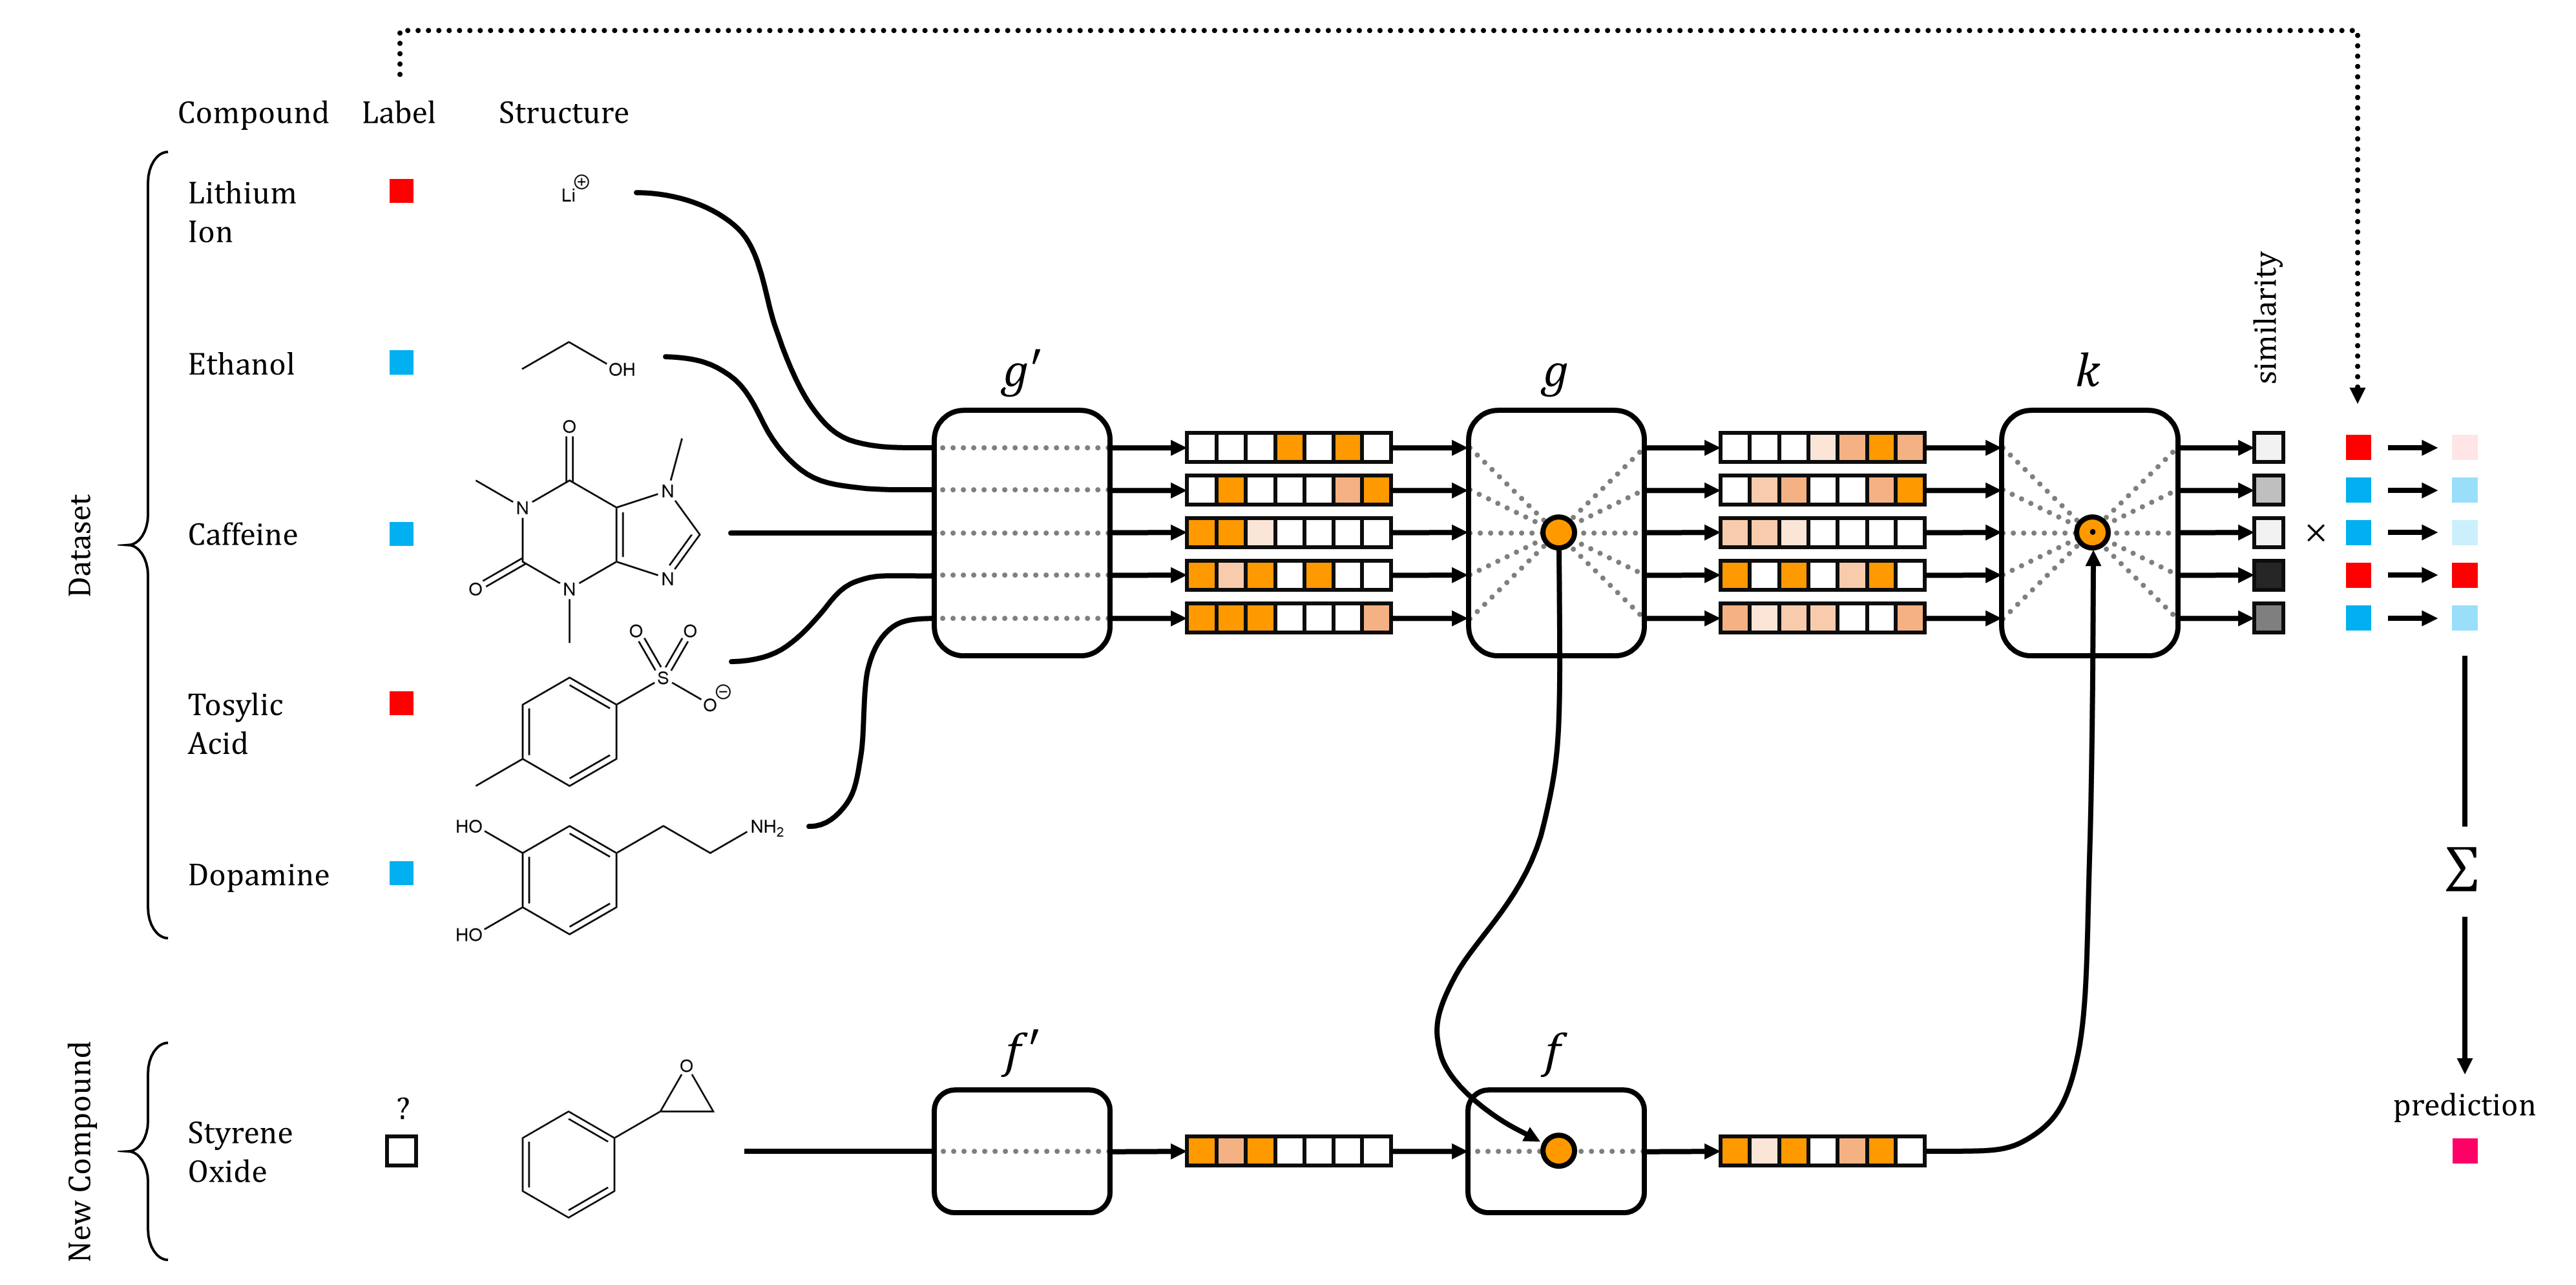
\includegraphics[width=\textwidth]{Images/schematic_v2.png}
\captionof{figure}{Schematic of Network Architecture for one-shot learning in drug discovery}
\label{fig:schematic}
\end{figure}

\subsubsection{Mathematical Formalism}

In this paper, we consider the situation in which one has multiple binary learning tasks. Some proportion of these tasks are reserved for training a one-shot learning model. The remaining tasks are those with too little data for standard machine-learning models to learn an effective classifier predicting the outcomes for these tasks (active/inactive correspond respectively to positive/negative examples for the binary classifier). The goal is to harness the information available in the training tasks to create strong classifiers for the test systems. 

%(The one-shot learning framework does not currently support low-data regression. It would be interesting for future work to extend the mathematical framework to do so. Han: I completely agree this is quite fascinating. Perhaps,  you could do a kernel average over the outcomes for regression. )

Mathematically, we have $T$ tasks, each associated with a data set, $S=\left\{\left(x_i,y_i\right)\right\}_{i=1}^{m}$, $y_i\in\left\{0,1\right\}$ (here $m = |S|$ is the number of datapoints in $S$). In our setting, each task typically corresponds to an experimental assay. The datapoints $x$ are compounds tested in the experimental assay, while the labels $y$ are binary experimental outcomes for the experiment (e.g. active/inactive). The learning challenge is learning to predict the experimental outcomes for new compounds tested against this assay.

We refer to the collection of available datapoints for a given task as a "support" set. The goal is to learn a function $h$, parameterized upon choice of support $S$ that predicts the probability of any query $x$ being active in the same system. Formally, $h_S(x)\,:\,\mathcal{X}\rightarrow\left[0,1\right]$, where $\mathcal{X}$ is the chemical space of small-molecules. If $h$ is specified with a neural network, fully differentiable with respect to $x$ \emph{and} $S$, then $h$ can be trained end-to-end with gradient descent.


\subsubsection{One-shot Learning}
In this section, we briefly review previously proposed techniques for one-shot learning and then introduce our new architecture for one-shot learning. We closely follow notation introduced in previous work \cite{vinyals2016matching} to lower notational burden for readers.
\paragraph{Review of prior one-shot techniques}

Deep one-shot learning systems \cite{santoro2016one, vinyals2016matching} use convolutional layers to encode images into continuous vectors. In the simplest one-shot learning formalism these continuous vectors are then fed into a simple nearest-neighbor classifier, that labels new examples by distance-weighted combination of support set labels. Let $a(x, x_i)$ denote some weighting function for query example $x$ and support set element $x_i$ with associated label $y_i$. Then the label $h_S(x)$ for query compound $x$ can be defined as
\[
h_S(x) = \sum\limits_{i=1}^{m}a\left(x,x_i\right)y_i
\]
The function $a$ is called an attention mechanism in previous work \cite{vinyals2016matching}. Mathematically, an attention mechanism is a non-negative function $a(x,x_i)$, with $\sum\nolimits_{i=1}^{m}a(x,x_i)=1$, that forms a probability distribution over the support set. The purpose of the attention distribution $a(x, \cdot)$ is to reflect the model's reasoning about the relationship between examples in support $S$ and the query $x$. The final prediction of the task's output for $x$ can then be interpreted as the expected value of the $y_i$'s under the attention distribution.

The attention mechanism $a$ depends on two embedding functions $f\,:\,\mathcal{X}\rightarrow\mathbf{R}^p$ and $g\,:\,\mathcal{X}\rightarrow\mathbf{R}^p$ which embed input examples (in small molecule space) into a continuous representation space. In past work, both $f$ and $g$ are standard convolutional networks, while in ours, $f$ and $g$ are graph-convolutional networks. The similarities between the ``embedded'' vectors $f(x)$ and $\{g(x_i)\}$ are computed using a similarity measure $k(\cdot,\cdot)$.  For example, $k$ could be the cosine-distance between two vectors. Given a choice of similarity measure, a simple attention mechanism $a$ can be defined by normalizing the similarity values
\[
a(x,x_i) = \frac{k\left(f(x),g(x_i\right))}{\sum\nolimits_{j=1}^{m} k\left(f(x),g(x_j\right))}
\]
Note that $a(x,x_i)$ is large when $f(x)$ is closer to $g(x_i)$ under metric $k$ compared to the other $g(x_j)$'s. This formulation of one-shot learning has been referred to as a Siamese one-shot learning method \cite{koch2015siamese}. If $f$ and $g$ are circular fingerprints\cite{rogers2010extended}, and $k$ the Tanimoto distance, notice that this formula matches standard chemoinformatic similarity methods.

% Example similarity functions include the exponentiated cosine similarity, $k(z,z^\prime)=e^{\cos\left(z,z^\prime\right)}$ or the RBF kernel, $k(z,z^\prime)=e^{-\|z - z^\prime|_2^2/2}$. 

The simple one-shot learning formulation introduced thus far uses independent embeddings $f(x)$ and $g(x_i)$ with only the distance metric $k$ linking the information from the two feature embeddings. As a result, the feature map $f(x)$ is formed without any context about data available in support $S = \{x_1,\dotsc, x_m\}$. The previously introduced matching-network architecture \cite{vinyals2016matching} addresses this problem by developing full context embeddings, in which embeddings $f(x)=f(x\mid S)$ and $g(x_i)=g(x_i\mid S)$ are computed using both $x$ and $S$. Full context embeddings allow the embeddings for $x$ and $x_i$'s to affect one another. Empirically, this modification allows for stronger one-shot learning results.

To construct $f(x\mid S)$ and $g(x_i\mid S$), matching networks\cite{vinyals2016matching} compute initial embeddings $f^\prime(x)$ and $g^\prime(x)$ using standard convolutional neural networks. (Note $f'$ and $g'$ are identical to the $f$ and $g$ used in the simple one-shot formulation.) The embedding $g(x)$ is computed by placing all the $g^\prime(x_i)$'s into a vector, and linking all the elements using a bidirectional LSTM \cite{hochreiter1997long, graves2013hybrid} ($\text{BiLSTM}$), allowing each $g(x_i)$ to be influenced by all the $g^\prime(x_j)$'s. 
\[
g(x\mid S) =\text{BiLSTM}([g'(x_1)|\cdots|g'(x_m)])
\]
We note that LSTM (long short-term memory) networks are a form of recurrent neural network useful for processing sequences of information. In our application, the support set $S$ can be viewed as a sequence $x_1,\dotsc, x_m$. The BiLSTM is a modification of the basic LSTM that partially reduces dependence of the output on the ordering of the sequence. 

To compute embedding $f(x\mid S)$, matching networks exploit a context based attention LSTM model \cite{vinyals2015order} ($\text{attLSTM}$), which is entirely order invariant with respect to the sequence. This model computes an order independent combination of its inputs.
\[
f(x\mid S) = \text{attLSTM}(f'(x), \{g(x_i\mid S)\})
\]
Internally, the $\text{attLSTM}$ contains $K$ layers of processing which allow for transfer of information amongst its input. Note that both the $\text{BiLSTM}$ and $\text{attLSTM}$ are mechanisms for combining sequences of vectors into single vectors. However, the $\text{attLSTM}$ is order-independent, while the $\text{BiLSTM}$ is order dependent. The order dependence in the definition of $g(x\mid S)$ is undesirable since there is no natural ordering to the elements of the support set. Furthermore, the treatment of $f$ and $g$ is non-symmetric. While $g(\cdot \mid S)$ depends only on the $g'$, the definition of $f$ depends on $f'$ and the embedding $g(\cdot \mid S)$. %A more natural architecture might insist upon a more symmetric ordering.


%Moreover, notice that $f$ is formed after $g$

%take $g^\prime(S)$ to be $\left[g^\prime(x_1)^\top,\dots,g^\prime(x_m)^\top\right]^\top$

\paragraph{Iterative refinement LSTMs}
\begin{figure}[h]
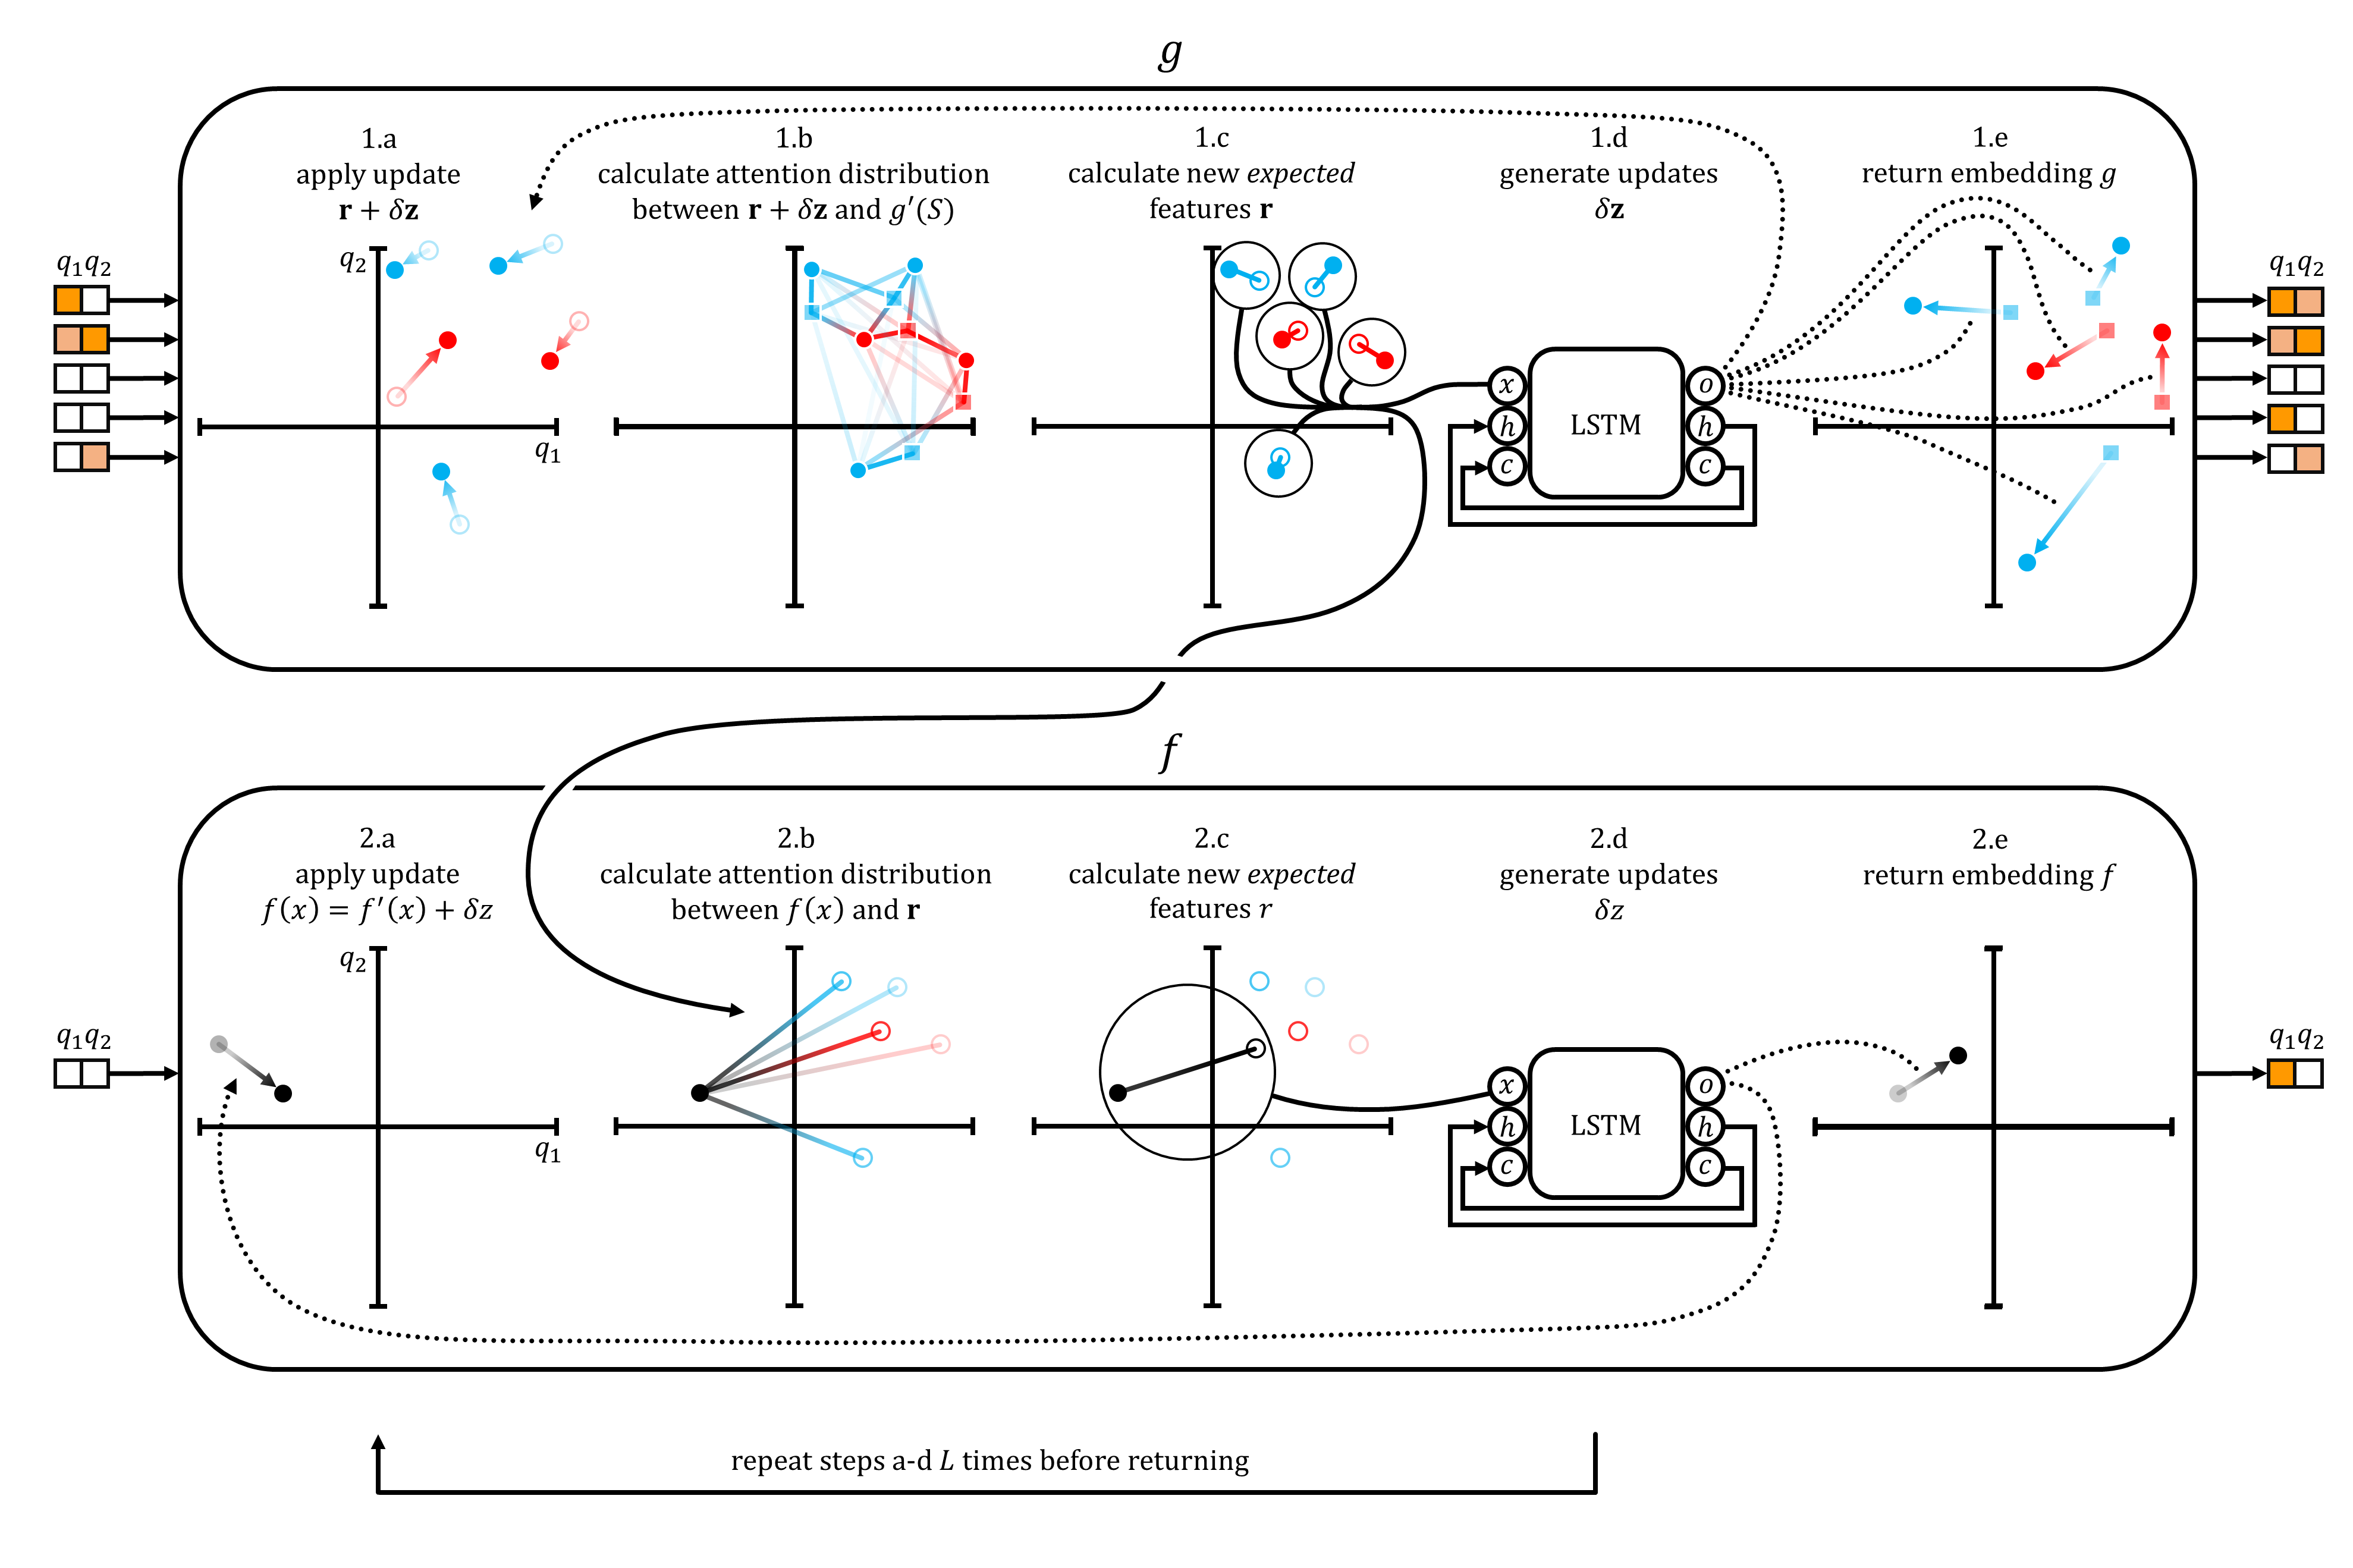
\includegraphics[width=\textwidth]{Images/resiembedding_graphic_v2.png}
\captionof{figure}{Pictorial depiction of iterative refinement of embeddings. Inputs/outputs are 2 dimensional for illustrative purposes, with $q_1$ and $q_2$ forming the coordinate axes. Red and blue points depict positive/negative samples (for illustrative purposes only). The original embedding $g'(S)$ is shown as squares. The expected features, $\mathbf{r}$ are shown as empty circles.}
\label{fig:resiembed}
\end{figure}

Our proposed architecture for one-shot learning preserves the context-aware design of matching networks, but resolves the order dependence in the support-embedding $g$ and the non-symmetric treatment of the query and support noted in the previous section (Figure~\ref{fig:resiembed}).

The core idea is to use an $\text{attLSTM}$ to generate both query embedding $f$ and support embedding $g$. As noted previously, the matching networks \cite{vinyals2016matching} embedding requires the support embedding $g(\cdot \mid S)$ to define $f(\cdot \mid S)$. To resolve this issue, our architecture iteratively evolves both embeddings simultaneously.

On the first iteration, we define $f(x) = f^\prime(x)$ and $g(S)= g^\prime(S)$. Then, we iteratively update the embeddings $f$ and $g$ for $L$ steps using an attention mechanism. This iteration for $L$ steps is analogous to the $K$ internal steps within an $\text{attLSTM}$, but with dual refinement of both support and query (Figure~\ref{fig:resiembed}). This construction allows the embedding of the data set to iteratively inform the embedding of the query. The quantity $L$ will be referred to as the depth of the IterRefLSTM. The equations below specify the full update performed over the $L$ iterations.

%(lines 1-3 below). For each example, the expected feature map under the attention mechanism is calculated, which is then fed alongside the initial embeddings into an LSTM, which generates changes to the original embedding. The process is then repeated with the new embedding for a fixed number of steps.
\begin{minipage}[b]{\linewidth}
\centering
\begin{tabular}{M M l}
        \multicolumn{4}{c}{\emph{Initialize}}\\
        \multicolumn{4}{c}{$\mathbf{r} = g^\prime(S)$\quad $\delta \mathbf{z} = \mathbf{0}$\quad $\delta z = 0$}\\       
        \multicolumn{4}{c}{\emph{Repeat L times}}\\
        e & k(f^\prime(x)+\delta z,\mathbf{r}) & \mathbf{e} & k(\mathbf{r}+\delta\mathbf{z},g^\prime(S)) & \mbox{(similarity measures)}\\
        a_j &  e_{j} / \sum\nolimits_{j=1}^{m}e_{ij} &  \mathbf{A}_{ij} &  \mathbf{e}_{ij} / \sum\nolimits_{j=1}^{m}\mathbf{e}_{ij} & \mbox{(attention mechanism)}\\        
        r & a^\top \mathbf{r} & \mathbf{r} & \mathbf{A} g^\prime(\mathbf{S}) &  \mbox{(expected feature map)}\\
        \delta z & {\rm{LSTM}}\left([\delta z,r]\right) & \delta \mathbf{z} & {\rm{LSTM}}\left([\delta \mathbf{z}, \mathbf{r}]\right) &  \mbox{(generate updates)}\\
        \multicolumn{4}{c}{\emph{Return}}\\
        f(x) & f^\prime(x) + \delta z & g(\mathbf{S}) & g^\prime(\mathbf{S})+\delta \mathbf{z} & \mbox{(evolve embeddings)}\\
\end{tabular}
\end{minipage}
\vspace{6pt}

The generated dually evolved embeddings are used to perform one-shot learning as in the simpler models explained in previous sections.

\subsubsection{Graph Convolutions}
We briefly review prior work on molecular graph convolution, then introduce a pair of new graph convolutional layers that we find useful for architectural design.

\paragraph{Review of prior work on molecular graph convolutions}
Earlier work \cite{duvenaud2015convolutional} defines a generalized graph convolution layer that extends standard two-dimensional convolutions upon images to arbitrary graphs. In standard convolutional networks, an image can be viewed as a grid, where each node corresponds to a pixel. The ``neighbors'' of a pixel in the same receptive field are passed through a dense neural layer to compute the output value for the convolution\cite{karpathy231n}. Similarly, when computing the convolution output for a specific node in an arbitrary graph, all neighbors of the node are passed through a dense layer to form the new features at this node. Both convolutions exploit the ``local geometry'' of the system to reduce the number of learnable parameters (see figure \ref{conv} and Appendix). Since molecules can be viewed as undirected graphs, with atoms as nodes and bonds as edges, graph convolutional architectures allow for the learning of complex functions of molecular structure.

Graph-convolutional networks are useful for transforming small-molecules into continuous vectorial representations. Such representations have emerged as a powerful way to manipulate small molecules within deep networks \cite{gomez2016automatic}. Earlier work on one-shot learning uses convolutional neural networks to encode images into continuous vectors which are then used to make one-shot predictions. By analogy, we use graph-convolutional neural networks to encode small-molecules in a form suitable for one-shot prediction.


\paragraph{New Layers}
For the purposes of architectural design, we found it useful to introduce a pair of graph convolutional layer types, max-pooling and graph-gathering. The max-pooling operation has been used widely in the broader convolutional architecture literature \cite{karpathy231n}, and the graph-gather layer has been used implicitly in previous graph-convolutional architectures \cite{duvenaud2015convolutional}.

Standard convolutional networks have "pooling layers", which perform a max operation upon local receptive fields in an image \cite{karpathy231n}. In analogy to this pooling operation, we introduce an analogous max pool operator on a node in graph structured data that simply returns the maximum activation across the node and the node's neighbors (see figure \ref{conv} and Appendix). Such an operation is useful for increasing the size of downstream convolutional layer receptive fields without increasing the number of parameters.

In a graph-convolutional system, each node has a vector of descriptors. However, at prediction time, we will require a single vector descriptor of fixed size for the entire graph. We introduce a graph-gather convolutional layer which simply sums all feature vectors for all nodes in the graph to obtain a graph feature vector (see figure \ref{conv}). Note that summing feature vectors in this fashion has been done in previous architectures \cite{duvenaud2015convolutional}, but we find that explicitly defining a graph-gather layer is useful for architectural design.


To facilitate the use of graph-convolutional layers in future work, we open-source our Tensorflow\cite{abadi2016tensorflow} implementation of graph-convolutions, graph-pooling, and graph-gathering layers as part of DeepChem \cite{ram2016}.

\begin{figure}[H]
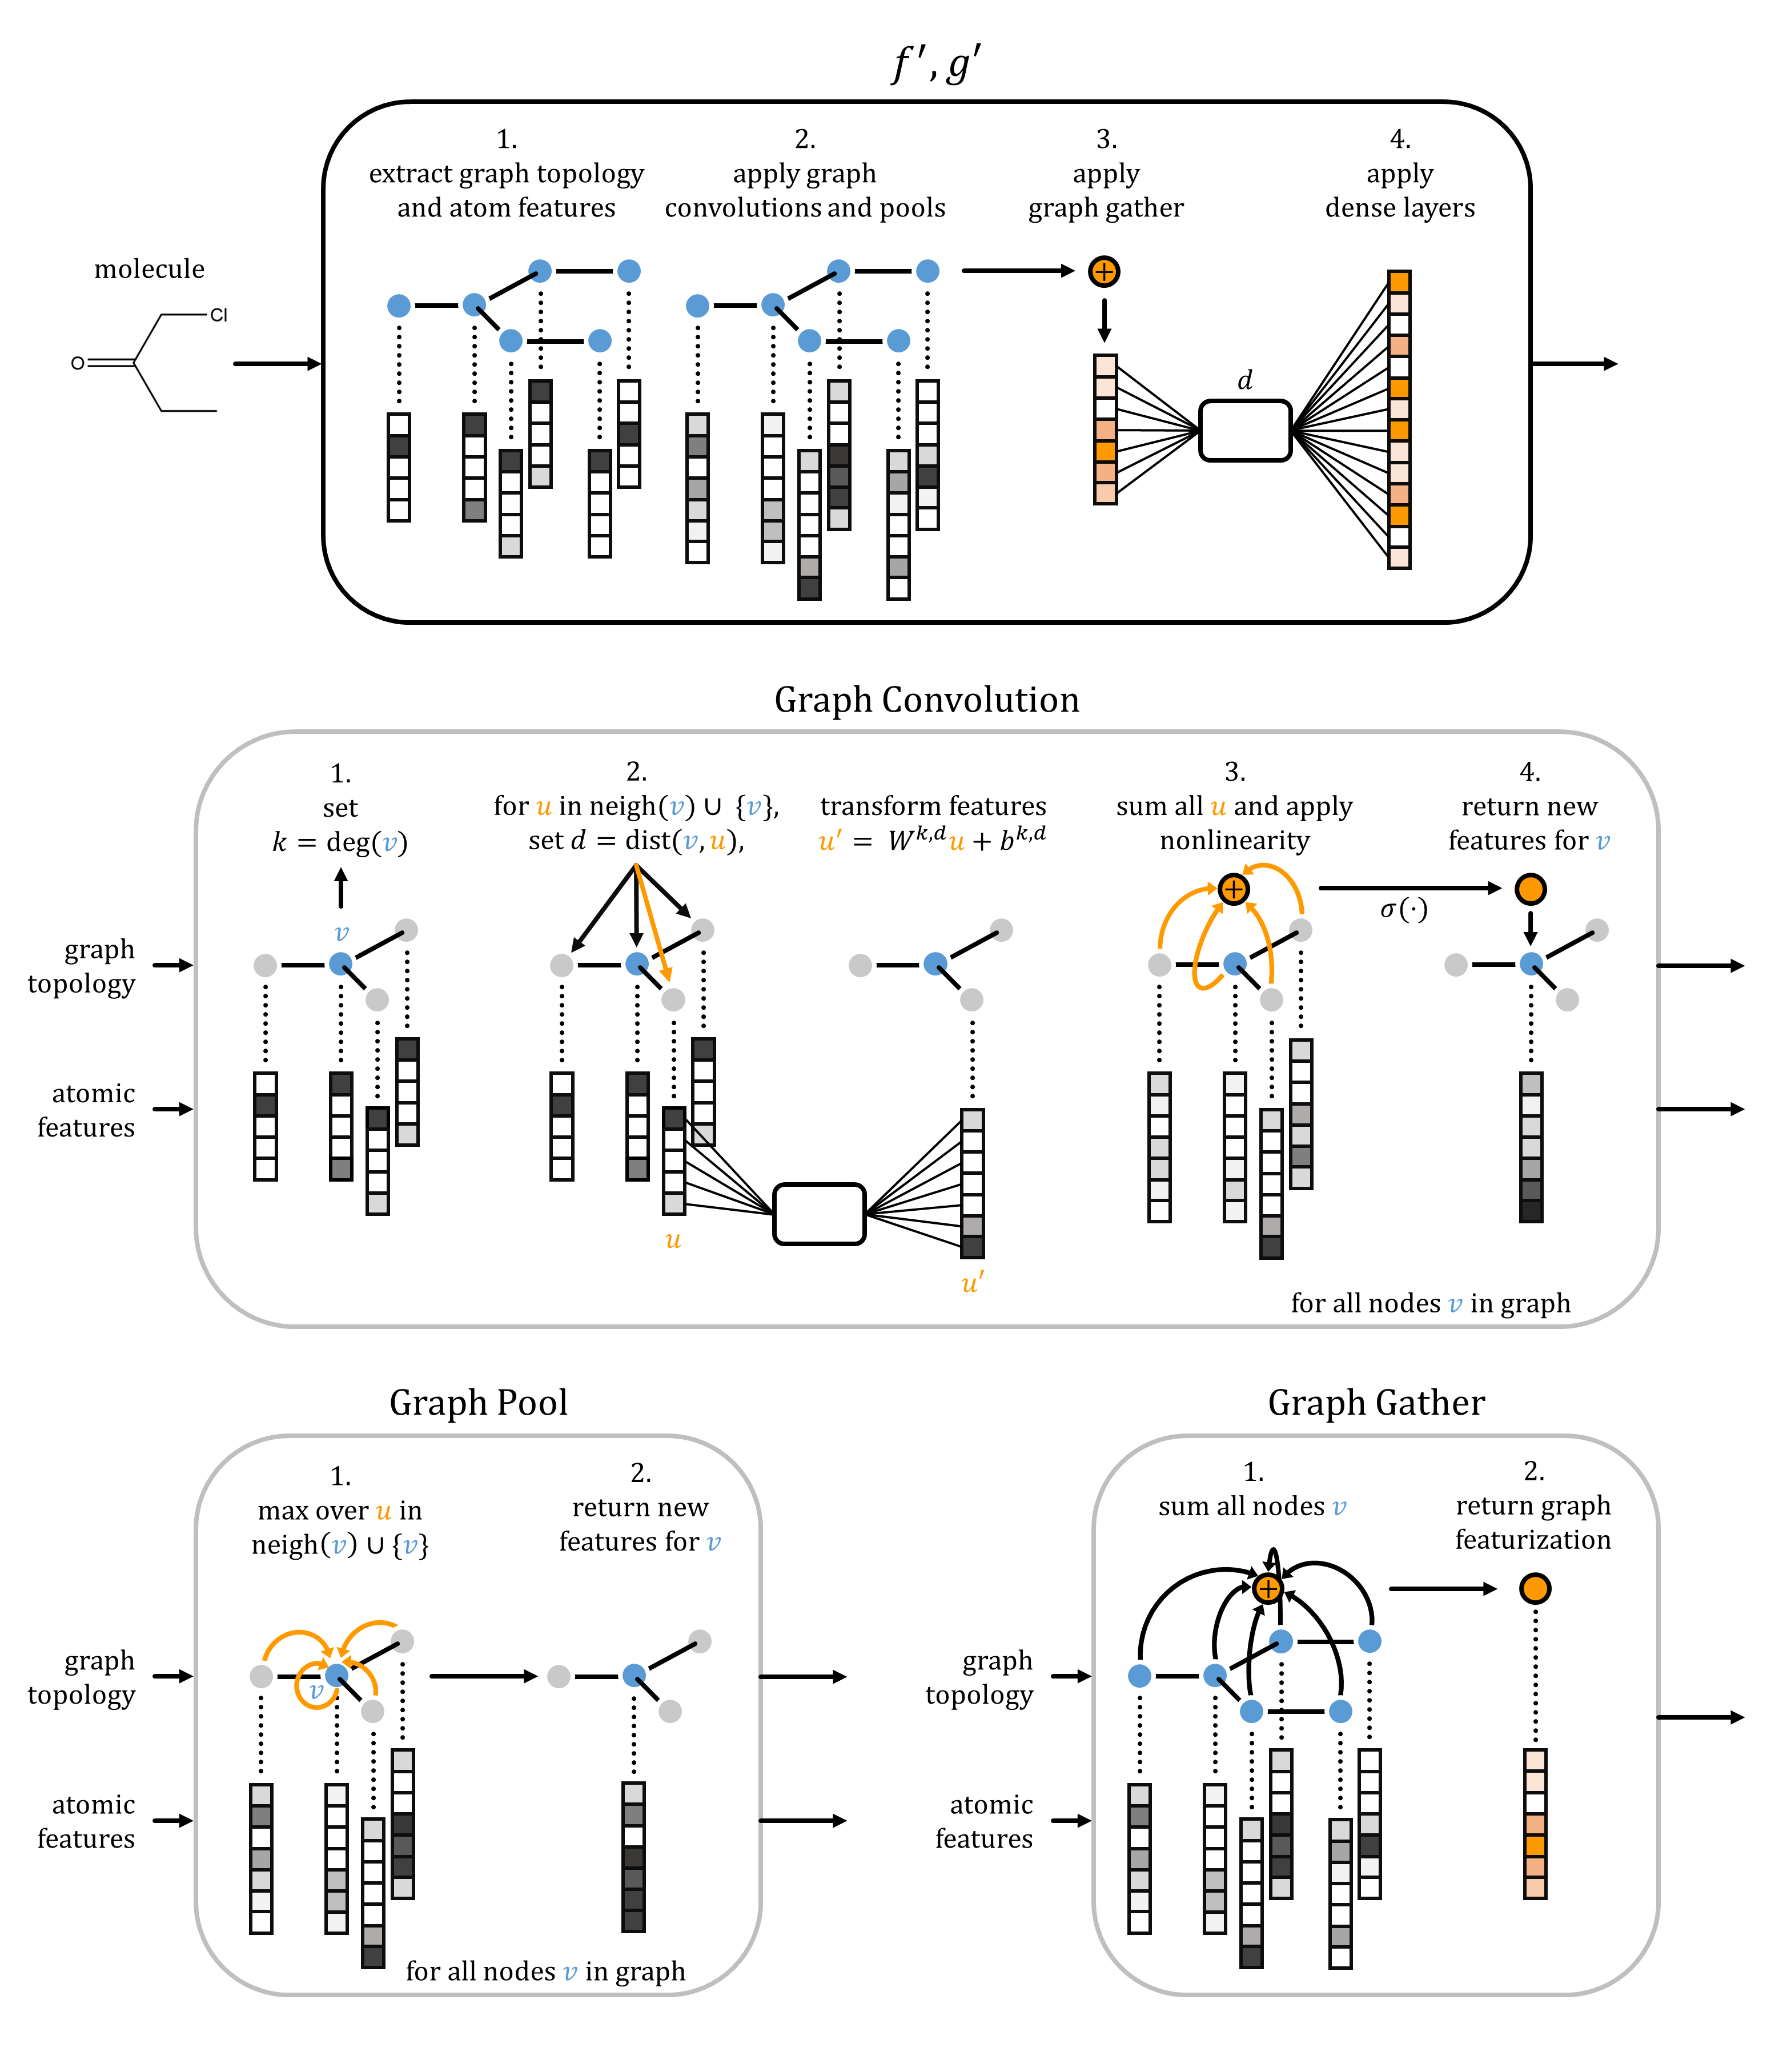
\includegraphics[width=\textwidth]{Images/graphconv_graphic_v2.png}
\captionof{figure}{Graphical representation of the major graph operations described in this paper. For each of the operations, the nodes being operated on are shown in blue, with unchanged nodes shown in light blue. For graph convolution and graph pool, the operation is shown for a single node, $v$, however, these operations are performed on all nodes $v$ in the graph simultaneously.}
\label{conv}
\end{figure}

%Furthermore, we modify the architecture in (\cite{duvenaud2015convolutional}) to more closely mirror the feedforward architectures commonly used in convolutional neural networks, such as those found in AlexNet (\cite{alex_net}) and LeNet (CITE).

\subsubsection{Model Training and Evaluation}
The objective for the iterative refinement LSTM models is similar to that for the matching networks, with the key difference that a set of training tasks are specified instead of a set of training classes. Note that this distinction means our work is not a direct extension of prior work on one-shot learning; rather we seek to demonstrate that one-shot methods are capable of transferring information between related, but distinct learning tasks. 

Let $\text{Tasks}$ represent the set of all learning tasks. We split this into two disjoint sets, $\text{Train-Tasks}$ and $\text{Test-Tasks}$. Let $S$ represent a support set, and let $B$ represent a batch of queries.
\[
\mathcal{L} = -E_{T\in\text{Train-Tasks}} \left [ E_{S\sim T, B\sim T} \left [ \sum_{(x,y) \in B} \log P_\theta(y\mid x, S) \right ] \right ]
\]

Training consists of a sequence of episodes. In each episode, a task $T$ is randomly sampled, then a support $S$ and a batch of queries $B$ (non-overlapping) are sampled from the task. One gradient descent step minimizing $\mathcal{L}$, using ADAM \cite{kingma2014adam} is performed for each episode. We experimented with more gradient descent steps per episode, but found that sampling more supports instead improved performance. The appendix contains numerical details of settings used for training.

At test time, the accuracy of a one-shot model is evaluated separately for each test task in $\text{Test-Tasks}$. For a given test task, a support of size $|S|$ is sampled at random from datapoints for that task. The ROC-AUC score for the model is evaluated on the remainder of the datapoints for the test task (excluding the support). This procedure is reported $n$ times for each test task ($20$ times in all experiments reported below), and the mean and standard deviations of ROC-AUC scores for each test task are computed. 
  

\subsection{Experiments}
This section reports experimental results for one-shot models across a number of assay collections.
\subsubsection{Tox21}
The Tox21 collection consists of 12 nuclear receptor assays related to human toxicity, first gathered for the Tox21 Data Challenge \cite{Tox21}. The winner of this challenge used a multitask deep-network \cite{unterthiner2015toxicity} to achieve strong predictive performance. For a low-data benchmark, we don't use the standard train/test split for this dataset. Instead, we use the first nine assays as the training set, and the last 3 assays as the test collection. For details, see appendix.

Results are in Table~\ref{tab:tox21}. All one-shot learning methods show strong boosts over the random-forest baseline, with the iterative refinement LSTM models showing a more robust boost in the presence of less data. Interestingly, the iterative refinement LSTM appears to display lower variance due to choice of support set when compared to other models, demonstrating a potential benefit of iterative refinement process. The singletask graph convolutional baseline performs much worse than all one-shot models, demonstrating that the strong performance of one-shot models likely requires architectures that explicitly promote metric learning.
\begin{table}[h]
    \centering
    \begin{tabular}{ |c|c|c|c|c|c| } 
    \hline
    Tox21 & RF (100 trees) & Graph Conv & Siamese & AttnLSTM & IterRefLSTM \\ 
    \hline
    10+/10- & $0.586 \pm 0.056$ & $0.648 \pm 0.029$ & $0.820 \pm 0.003$ & $0.801 \pm 0.001$ & $\mathbf{0.823 \pm 0.002}$ \\
    \hline
    5+/10- & $0.573 \pm 0.060$ & $0.637 \pm 0.061$ & $0.823 \pm 0.004$ & $0.753 \pm 0.173$ & $\mathbf{0.830 \pm 0.001}$ \\ 
    \hline
    1+/10- & $0.551 \pm 0.067$ & $0.541 \pm 0.093$ & $\mathbf{0.726 \pm 0.173}$ & $0.549 \pm 0.088$ & $0.724 \pm 0.008$ \\ 
    \hline
    1+/5- & $0.559 \pm 0.063$ & $0.595 \pm 0.086$ & $0.687 \pm 0.210$ & $0.593 \pm 0.153$ & $\mathbf{0.795 \pm 0.005}$ \\ 
    \hline
    1+/1- & $0.535 \pm 0.056$ & $0.589 \pm 0.068$ & $0.657 \pm 0.222$ & $0.507 \pm 0.079$ & $\mathbf{0.827 \pm 0.001}$\\ 
    \hline
    \end{tabular}
    \caption{ROC-AUC scores of models on median held-out task for each model on Tox21. Numbers reported are means and standard deviations. Randomness is over the choice of support set; experiment is repeated with 20 support sets. The appendix contains results for all held-out Tox21 tasks. The result with highest mean in each row is highlighted. The notation 10+/10- indicates supports with $10$ positive examples and $10$ negative examples.}
    \label{tab:tox21}
\end{table}

\subsubsection{SIDER}

The SIDER dataset contains information on marketed medicines and their observed adverse reactions \cite{kuhn2015sider}. We originally tested on the original 5868 side effect categories, but due to lack of signal at this level of granularity we grouped the drug-SE pairs into 27 system organ classes according to MedDRA classifications \cite{meddra}. We treat the problem of predicting whether a given compound induces a side-effect as an individual task (for 27 tasks in total). For the low-data benchmark, all models were trained on the first 21 tasks and tested on the last 6. For details see appendix.

Results are in Table~\ref{tab:sider}. The Siamese and IterRefLSTM methods show strong boosts over the random-forest baseline, but the AttnLSTM has poor performance on this collection (comparable to the random forest). The iterative refinement LSTM models show a robust boost in the presence of less data. As before, the iterative refinement models tend to have lower variance. The graph convolutional baseline does poorly, with performance indistinguishable from random.

\begin{table}
    \centering
    \begin{tabular}{ |c|c|c|c|c|c| } 
    \hline
    SIDER & RF (100 trees) & Graph Conv & Siamese & AttnLSTM & IterRefLSTM \\ 
    \hline
    10+/10- & $0.535 \pm 0.036$ & $0.483 \pm 0.026$ & $\mathbf{0.687 \pm 0.089}$ & $0.553 \pm 0.058$ & $0.669 \pm 0.007$ \\
    \hline
    5+/10- & $0.533 \pm 0.030$ & $0.473 \pm 0.029$ & $0.648 \pm 0.070$ & $0.534 \pm 0.053$ & $\mathbf{0.704 \pm 0.002}$ \\ 
    \hline
    1+/10- & $0.540 \pm 0.034$ & $0.447 \pm 0.016$ & $0.544 \pm 0.056$ & $0.506 \pm 0.016$ & $\mathbf{0.556 \pm 0.011}$ \\ 
    \hline
    1+/5- & $0.529 \pm 0.028$ & $0.457 \pm 0.029$ & $0.530 \pm 0.050$ & $0.505 \pm 0.022$ & $\mathbf{0.644 \pm 0.012}$ \\ 
    \hline
    1+/1- & $0.506 \pm 0.039$ & $0.468 \pm 0.045$ & $0.510 \pm 0.016$ & $0.501 \pm 0.022$ & $\mathbf{0.697 \pm 0.002}$ \\ 
    \hline
    \end{tabular}
    \caption{ROC-AUC scores of models on median held-out task for each model on SIDER. Numbers reported are means and standard deviations. Randomness is over the choice of support set; experiment is repeated with 20 support sets. The appendix contains results for all held-out SIDER tasks. The result with highest mean in each row is highlighted. The notation 10+/10- indicates supports with $10$ positive examples and $10$ negative examples.}
    \label{tab:sider}
\end{table}

\subsubsection{MUV}
The MUV dataset collection \cite{rohrer2009maximum} contains 17 assays designed to be challenging for standard virtual screening. The positives examples in these datasets are selected to be structurally distinct from one another. As a result, this collection is a best-case scenario for baseline machine learning (since each data point is maximally informative) and a worst-case test for the low-data methods, since structural similarity cannot be effectively exploited to predict behavior of new active compounds.

Results are in Table~\ref{tab:MUV}. The random forest baseline does significantly better for MUV than for the other two datsets we tested. All one-shot models struggle on this collection. The graph-convolutional baseline struggles on MUV as well, suggesting that part of the difficulty of MUV may be due to current limitations of graph convolutions. That said, these results suggest that one-shot learning methods may have some difficulties generalizing to new molecular scaffolds.

\begin{table}
    \centering
    \begin{tabular}{ |c|c|c|c|c|c| } 
    \hline
    MUV & RF (100 trees) & Graph Conv & Siamese & AttnLSTM & IterRefLSTM \\ 
    \hline
    10+/10- & $\mathbf{0.754 \pm 0.064}$ & $0.568 \pm 0.085$ & $0.601 \pm 0.041$ & $0.504 \pm 0.058$ & $0.499 \pm 0.053$ \\
    \hline
    5+/10- & $\mathbf{0.730 \pm 0.063}$ & $0.565 \pm 0.068$ & $0.655 \pm 0.166$ & $0.507 \pm 0.052$ & $0.663 \pm 0.019$ \\ 
    \hline
    1+/10- & $0.556 \pm 0.084$ & $0.569 \pm 0.061$ & $\mathbf{0.602 \pm 0.118}$ & $0.504 \pm 0.044$ & $0.569 \pm 0.012$ \\ 
    \hline
    1+/5- & $0.598 \pm 0.067$ & $0.554 \pm 0.089$ & $0.514 \pm 0.053$ & $0.515 \pm 0.021$ & $\mathbf{0.632 \pm 0.011}$ \\ 
    \hline
    1+/1- & $\mathbf{0.559 \pm 0.095}$ & $0.552 \pm 0.084$ & $0.500 \pm 0.0001$ & $0.500 \pm 0.027$ & $0.479 \pm 0.037$ \\ 
    \hline
    \end{tabular}
    \caption{ROC-AUC scores of models on median held-out task for each model on MUV. Numbers reported are means and standard deviations. Randomness is over the choice of support set; experiment is repeated with 20 support sets. The appendix contains results for all held-out MUV tasks. The result with highest mean in each row is highlighted. The notation 10+/10- indicates supports with $10$ positive examples and $10$ negative examples.}
    \label{tab:MUV}
\end{table}

\subsubsection{Transfer Learning to SIDER from Tox21}

The experiments thus far have tested the ability of one-shot learning methods to generalize from training tasks to closely related testing tasks. To test whether one-shot learning methods are capable of broader generalization, we trained models on the Tox21 dataset collection and evaluated predictive accuracy on the SIDER collection. Note that these collections are broadly distinct, with Tox21 measuring results in nuclear receptor assays, and SIDER measuring adverse reactions from real patients.

Results are in Table~\ref{tab:transfer}. None of our models achieve any predictive power on this task, providing evidence that the one-shot models have limited generalization powers to unrelated systems.

\begin{table}
    \centering
    \begin{tabular}{ |c|c|c|c| } 
    \hline
    SIDER from Tox21 & Siamese & AttnLSTM & IterRefLSTM \\ 
    \hline
    10+/10- & $0.511 \pm 0.031$ & $0.509 \pm 0.014$ & $0.509 \pm 0.012$ \\
    \hline
    \end{tabular}
    \caption{ROC-AUC scores of models trained on Tox21 on median SIDER task for each model on SIDER. Note that models are evaluated on all SIDER tasks and not just the held-out SIDER tasks from previous section. Numbers reported are means and standard deviations. Randomness is over the choice of support set; experiment is repeated with 20 support sets. The result with highest mean in each row is highlighted. The notation 10+/10- indicates supports with $10$ positive examples and $10$ negative examples.}
    \label{tab:transfer}
\end{table}


\clearpage

\subsubsection*{Acknowledgments}

We would like to thank the Stanford Computing Resources for providing us with access to the Sherlock and Xstream GPU clusters. Thanks to David Duvenaud for useful preliminary discussions.

B.R. was supported by the Fannie and John Hertz Foundation.
%\bibliography{paper.bib}

\newpage
\section*{For Table of Contents Use Only}
{\huge \centering Low Data Drug Discovery with One-shot Learning}

{\Large Han Altae-Tran*, Bharath Ramsundar*, Aneesh S. Pappu, Vijay Pande}

* equal contribution

\begin{figure}[H]
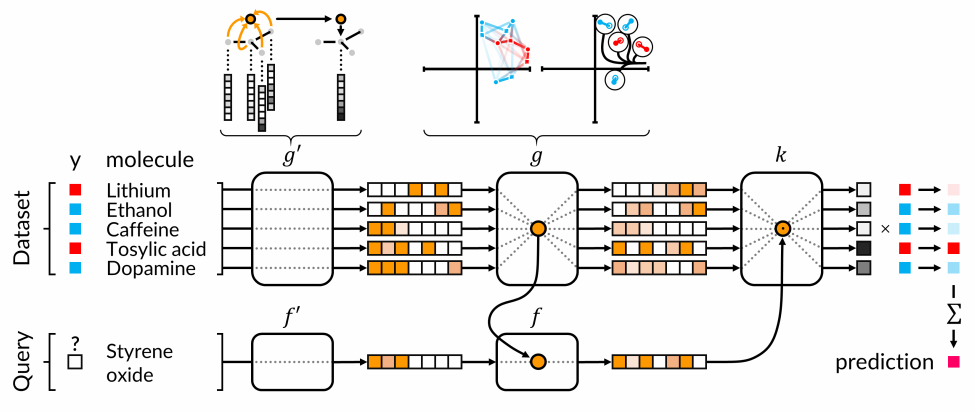
\includegraphics{Images/For_Table_Of_Contents_Only.png}
\end{figure}

Synopsis: We demonstrate how one-shot learning can lower the amount of data required to make meaningful predictions in drug discovery. Our architecture, the iterative refinement LSTM, permits the learning of meaningful distance metrics on small-molecule space.


%\end{document}

%\clearpage
%\section{Atomic Convolutional Networks for Predicting Protein-Ligand Binding Affinity}

\subsection{Abstract}
Empirical scoring functions based on either molecular force fields or cheminformatics descriptors are widely used, in conjunction with molecular docking, during the early stages of drug discovery to predict potency and binding affinity of a drug-like molecule to a given target.  These models require expert-level knowledge of physical chemistry and biology to be encoded as hand-tuned parameters or features rather than allowing the underlying model to select features in a data-driven procedure.  Here, we develop a general 3-dimensional spatial convolution operation for learning atomic-level chemical interactions directly from atomic coordinates and demonstrate its application to structure-based bioactivity prediction.  The atomic convolutional neural network is trained to predict the experimentally determined binding affinity of a protein-ligand complex by direct calculation of the energy associated with the complex, protein, and ligand given the crystal structure of the binding pose. Non-covalent interactions present in the complex that are absent in the protein-ligand sub-structures are identified and the model learns the interaction strength associated with these features. We test our model by predicting the binding free energy of a subset of protein-ligand complexes found in the PDBBind dataset and compare with state-of-the-art cheminformatics and machine learning-based approaches.  We find that all methods achieve experimental accuracy (less than 1 kcal/mol mean absolute error) and that atomic convolutional networks either outperform or perform competitively with the cheminformatics based methods. Unlike all previous protein-ligand prediction systems, atomic convolutional networks are end-to-end and fully-differentiable.  They represent a new data-driven, physics-based deep learning model paradigm that offers a strong foundation for future improvements in structure-based bioactivity prediction. 

\subsection{Introduction}


The success rate of the initial phases of drug discovery depends on the prediction, or measurement, of the affinity of a candidate ligand for a therapeutic target (e.g., protein) of interest. The space of synthetically accessible small molecules is unfathomably vast, estimated at over $10^{60}$ compounds \cite{virshup2013stochastic}. While exploring this entire space is currently computationally intractable, this combinatorial explosion underscores a core challenge in drug discovery: testing the affinity of as many small molecules as possible while maintaining a sufficient degree of accuracy. There is currently a significant trade-off in both experimental and computational drug screening approaches between speed, cost, and accuracy.\cite{dragiev2011systematic, wang2015accurate, trott2010autodock}

The introduction of machine learning into drug discovery pipelines has improved virtual drug screening as well as other physics-based evaluations of small molecules. Models such as random forests, logistic regression, and support vector machines \cite{svetnik2003random} have been used  extensively in virtual screening and chemoinformatics in the past decade and beyond. However, such models were beset by a fundamental limitation: the need to represent molecules with hand-curated, fixed-length vector features.

More recently, deep learning has demonstrated the potential to exceed this inherent limitation in traditional machine learning. The flexibility of deep neural networks allows models in principle to ``learn" successively higher orders of features from the simplest possible representations of the data at hand. In the computer vision field, for example, convolutional neural networks \cite{krizhevsky2012imagenet} applied to images can learn how to detect edges in early layers in the network; eyes, ears, etc. in intermediate network layers; and finally faces in terminal layers of the network. While such advanced artificial neural network frameworks have led to immense advances in the fields of computer vision and natural language processing, they have only recently penetrated other areas. 

The promise of DNNs has only just begun to be realized in the fields of chemistry and physics. Scientists have demonstrated the use of neural networks for molecular force fields \cite{behler2007nnpes,behler2011atomnn}, prediction of electronic properties of small molecules \cite{montavon2013machine}, protein-ligand binding \cite{durrant2011nnscore, wallach2015atomnet,ragoza2016protein}, chemoinformatics \cite{duvenaud2015convolutional, kearnes2016molecular, altae2016low}, among others. Previous works that addressed protein-ligand binding have used simpler, fully connected neural networks based on hand-curated features \cite{durrant2011nnscore} or used a direct application of voxel-based convolutional neural networks in the two-class classification task of distinguishing small molecule binders from non-binders. \cite{wallach2015atomnet,ragoza2016protein}  The atomic convolution architecture was inspired by the atomic fingerprint neural network, originally proposed by Behler and Parrinello \cite{behler2007nnpes,behler2011atomnn} for the purpose of fitting potential energy surfaces, with several key differences.  Rather than choose fixed parameters for the featurization of molecules into atomic fingerprint vectors, we optimize these parameters simultaneously with the neural network in an end-to-end fashion to allow the model to make data-driven decisions on features that are important to predicting ligand binding.  In addition, we utilize a neighbor list routine to reduce the computational cost of model training and evaluation, allowing the models to scale well to large systems.  This work represents the largest application of this method to date and the first application based purely on experimental data.

In this paper, we introduce a new fundamental deep learning primitive to improve the representational and predictive power for molecular systems, the Atomic Convolutional Neural Network (ACNN). Analogous to the original CNNs \cite{krizhevsky2012imagenet, lecun1995comparison}, ACNN's directly exploit the local three-dimensional structure of molecules to hierarchically learn more complex chemical features by optimizing both the model and featurization simultaneously in an end-to-end fashion.
Whereas many previous works focus on two-class classification of drug binding or non-binding, we apply ACNNs to directly predict binding free energy arising from non-covalent interactions purely from experimental data by direct integration of a ligand-binding thermodynamic cycle into the model optimization.  The resulting optimized energy function is size-extensive and fully-differentiable with respect to atomic coordinates.  In addition, ACNN models have the desirable feature of being able to generalize to larger systems than those it has been trained on.  After describing the mathematical architecture of the ACNNs, we report their application for the prediction of protein-ligand binding affinity with the publicly available PDBBind dataset. \cite{wang2005pdbbind}  All calculations were done in the open-source molecular machine learning package DeepChem.\cite{deepchem}  We open source all datasets and code required to reproduce this work.

\subsection{Methods}

\subsubsection{Atomic Convolutional Neural Networks}
The architecture of the atomic convolutional neural network is shown in Figure~\ref{fig:atomic_conv}.  We introduce two new primitive convolutional operations, atom type convolution and radial pooling. The atom type convolution makes use of a neighbor-listed distance matrix to extract features encoding local chemical environments from an input representation (Cartesian atomic coordinates) that does not necessarily contain spatial locality.
\begin{figure}
    \centering
    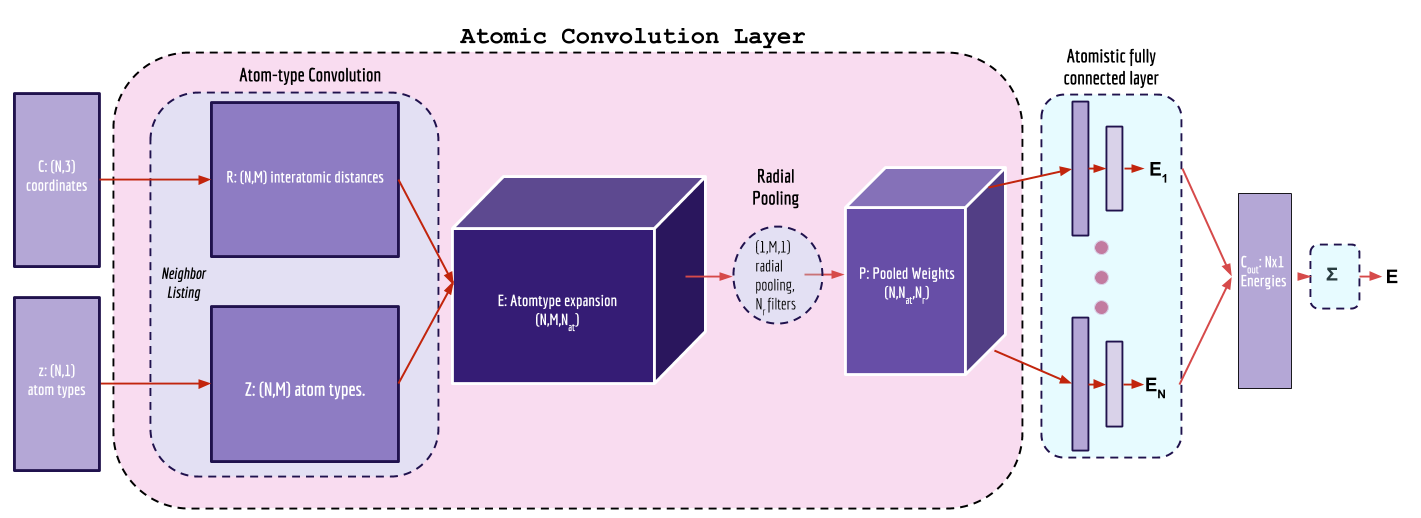
\includegraphics[width=\textwidth]{Images/Atomic_Conv_Diagram_rev3.png}
    \caption{Schematic of atomic convolution layer.}
    \label{fig:atomic_conv}
\end{figure}

\paragraph{Distance matrix and neighbor list construction}
The distance matrix $R$ and atomic number matrix $Z$ are constructed from the Cartesian atomic coordinates $X$.  We use a neighbor list routine \cite{yip1989neighbor} to reduce the complexity of this step from $O(N^2)$ to $O(NM)$, where $M$ is some maximum number of neighbors.  The radial interaction cutoff used in the neighbor list routine is 12 Å and the neighbor list is truncated at number of neighbors $M$, typically 12.  The initial neighbor list distance matrix representation is invariant to rigid body translation and rotation of the molecular system but not atom index or neighbor list atom index permutation.

The distance matrix construction accepts as input a $(N,3)$ coordinate matrix $C$. This matrix is ``neighbor listed'' into a $(N,M)$ matrix $R$. For atom $i$, the neighbor listing process finds the $M$ atoms closest to $i$ spatially. Let $N_i = [a_{i_1},\dotsc,a_{i_m}]$ be the list of neighbors. Then $R_{i,j}$ is defined as
\begin{eqnarray*}
R_{i,j} &= \|C_i - C_{i_j}\|_2
\end{eqnarray*}
The neighbor listing operation also constructs from the $(N,1)$ atomic number vector $z$ a $(N,M)$ matrix $Z$ which lists the atomic number of neighboring atoms (atom types).
\begin{equation*}
Z_{i,j} = \textrm{Atom type of }a_{i_j}
\end{equation*}

\paragraph{Atom type convolution} 
The output of the atom type convolution is constructed from the distance matrix $R$ and atomic number matrix $Z$. The matrix $R$ is fed into a (1x1) filter with stride 1 and depth of $N_\textrm{at}$, where $N_\textrm{at}$ is the number of unique atomic numbers (atom types) present in the molecular system.  The atom type convolution kernel is a step function that operates on neighbor distance matrix $R$:
\begin{equation*}
E_{i, j, k} = (K*R)_{i, j} = R_{i,j}K_{i,j}^k
\end{equation*}
where 
\begin{equation*}
K_{i,j}^k = \begin{cases} 
      1 & Z_{i,j} = N_k \\
      0 & \textrm{otherwise}
   \end{cases}
\end{equation*}
where $N_a$ is the atomic number of atom type $a$ ($a = 1,\dotsc,N_\textrm{at}$).  The atom type convolution layer is applied to the neighbor distance matrix to create output matrix $E$ of shape $(N, M, N_\textrm{at})$. The atom type convolution can also be thought of as an expansion layer that one-hot encodes the atom type $N_{a}$ into separate copies of the distance matrix $R_{N_{a}}$.
\paragraph{Radial pooling layer}
Radial pooling is a dimensionality reduction process intended to down-sample the output of the atom type convolution. This dimensionality reduction is done in part to prevent over-fitting by providing an abstracted form of the representation through feature binning, as well as reducing the number of parameters learned.  In addition, radial pooling provides an output representation invariant to neighbor list atom index permutation.  

Radial pooling takes input tensor $E$ output by the atom-type convolution of shape $(N,M,N_{at})$. Radial pooling is then performed by applying a radial filter over non-overlapping sub-regions of the input representation.  Mathematically, radial pooling layers pool over tensor slices (receptive fields) of size (1x$M$x1) with stride $1$ and a depth of $N_r$, where $N_r$ is the number of desired radial filters.  Radial pooling filters are of the functional form $f_s$

\begin{eqnarray*}
f_s(r_{i,j}) &= \exp\left(-\frac{(r_{i,j} - r_s)^2}{\sigma_s^2}\right)f_c(r_{i,j})\\
f_c(r_{i,j}) &= \begin{cases} 
      \frac{1}{2}\cos\left (\frac{\pi r_{i,j}}{R_c}\right) + 1 & 0 < r_{i,j} < R_c \\
      0 & r_{i,j} \geq R_c
   \end{cases}
\end{eqnarray*}

\begin{eqnarray*}
f_{i, j} = \sum_{n=1}^M \exp\left(-\frac{(r_{i,n} - r_{s,j})^2}{\sigma_{s,j}^2}\right)f_c(r_{i,n})\delta(Z_n - Z_j)
\end{eqnarray*}

Parameters $r_s$ and $\sigma_s$ are learn-able parameters for pooling function $f_s$. Parameter $R_c$ is the radial interaction cutoff, which is fixed to 12 Å.  Then, the output pooled matrix $P$ is of shape $(N,N_\textrm{at},N_r)$ and has entries
\begin{eqnarray*}
P_{i,n_a,n_r} = \beta_{n_r} \sum_{j=1}^M f_{n_r}(E_{i,j,k}) + b_{n_r}
\end{eqnarray*}
where $\beta_{n_r}$ is the non-learn-able scaling constant and $b_{n_r}$ is a non-learn-able bias constant.  Conceptually, applying radial pooling following an atom type convolution layer produces features which sum the pairwise-interactions between atom $i$ with atom type $a_i$ (e.g. H, C, N, etc.) and all neighboring atoms of type $a_j$ (e.g. H-H, H-C, H-N, etc.). 

\paragraph{Atomistic fully connected network}
The output $P$ of the radial pooling layer has shape $(N,N_\textrm{at}, N_r)$. We flatten the coordinates for each atom to obtain a tensor of shape $(N, N_\textrm{at}\cdot N_r)$. Atomic convolution layers can be stacked by feeding the flattened output of the radial pooling layer back into the atom-type convolution operation. Finally, we feed the tensor row-wise (per-atom) into a fully-connected network. The same fully connected weights and biases are used for each atom in a given molecule. The output of the atomistic fully-connected network is energy $E_i$ of atom $i$ ($i=1\cdots N$).  The total energy of the molecule, $E = \sum_i E_i$, is the sum of the atomic energies and is consequently invariant to atom index permutation.  Since the fully connected network input dimension only depends on the number of features, not number of atoms, a fully trained ACNN model can generalize to systems larger than those contained in the training set, given a fixed number of atom types and radial pooling filters.

\subsubsection{Application of atomic convolution networks to predicting protein-ligand binding affinity}
\begin{figure}[h]
  \centering
  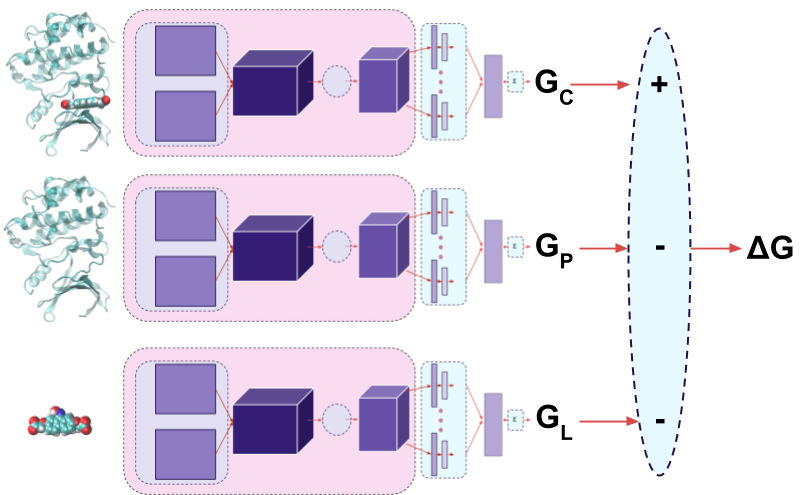
\includegraphics[width=.8\textwidth]{Images/pldiagram2.png}
  \caption{Diagram of Atomic Convolutions on Protein Ligand Systems.}
  \label{fig:protein_ligand}
\end{figure}
The atomic convolution network architecture produces an energy that is size-extensive and differentiable with respect to atomic positions. In order to learn non-covalent interactions using the atomic convolution energy function, we integrate the following thermodynamic cycle into the learning process
\begin{eqnarray*}
\Delta G_\textrm{complex} = G_\textrm{complex} - G_\textrm{protein} - G_\textrm{ligand}
\end{eqnarray*}

To create a model which can accurately predict $\Delta G_{\textrm{complex}}$, we create three weight-sharing, replica networks, one each for complex, protein, and ligand (Figure~\ref{fig:protein_ligand}). The full system is trained against the loss
\[\mathcal{L} = (\Delta G_\textrm{complex} - y_\textrm{complex})^2\]
Note how the complete network incorporates the thermodynamic cycle as a subcomponent. This system is trained end-to-end to predict $\Delta G$, but does so in a fashion which respects the underlying adsorption thermodynamics.  ACNN models were trained with stochastic gradient descent with a batch size of 24 and the ADAM optimizer \cite{kingma2014adam} for 100 epochs.

\subsubsection{Baseline Comparison}
\paragraph{Grid Featurizer Method}
The grid featurization method (GRID), first introduced in molecular machine learning benchmark MoleculeNet \cite{wu2017moleculenet}, was chosen as the baseline method for comparison of structure-based machine learning methods. The GRID method incorporates both the ligand and target protein structural information by considering both the chemical interaction within the binding pocket as well as features of the protein and ligand individually. The grid featurizer was inspired by the NNscore featurizer \cite{durrant2011nnscore} and SPLIF \cite{da2014splif} but optimized for speed, robustness, and generalizability. The molecular interactions enumerated by the GRID method include salt bridges and hydrogen bonding between protein and ligand, intra-ligand circular fingerprints\cite{rogers2010extended}, intra-protein circular fingerprints, and protein-ligand SPLIF fingerprints.

The features produced by GRID were used to create a random forest regression model (GRID-RF) and a fully-connected neural network model (GRID-NN). Random forest models were trained using the scikit-learn \texttt{RandomForestRegressor}.  Fully-connected neural network models were trained using the DeepChem \texttt{†MultitaskRegressor}. Model hyperparameters are described elsewhere \cite{wu2017moleculenet}.  The GRID method in conjunction with the random forest regression model is currently the top performing machine learning method for structure-based binding affinity prediction on the PDBBind dataset contained within the MoleculeNet benchmark.

\paragraph{Graph Convolution Method}

The graph convolutional neural network (GCNN) of Duvenaud and Maclaurin\cite{duvenaud2015convolutional} was chosen as a baseline for ligand-based convolutional deep learning methods.  Graph convolutional models treat molecules as undirected graphs whose vertices and edges represent individual atoms and bonds. A graph convolutional layer applies the same learnable function to every atom in the graph, resulting in a learned featurization. The graph convolutional algorithm is similar in spirit to the ACNN, but uses the bonded connectivity graph instead of a spatial neighbor list. Put another way, the GCNN is purely two dimensional, while the ACNN is natively a three dimensional architecture. Descriptions of the graph convolutional models and model hyperparameters are given elsewhere in the literature \cite{wu2017moleculenet}.

\paragraph{ECFP Fingerprint Method}

The extended-connectivity fingerprints\cite{rogers2010extended} (ECFP) featurization method was chosen as a baseline for ligand-based machine learning methods.  ECFPs are widely-used molecular characterizations in chemical informatics. The ECFP featurization process decomposes a  molecule into segments originated from non-hydrogen atoms, each assigned with a unique identifier. These segments and identifiers are extended through bonds to generate larger substructures and corresponding identifiers. The substructures are hashed into a fixed length binary fingerprint.

The features produced by ECFP were used to create a random forest regression model (ECFP-RF) and a fully-connected neural network model (ECFP-NN). Random forest models were trained using the scikit-learn \texttt{RandomForestRegressor}.  Fully-connected neural network models were trained using the DeepChem \texttt{TensorflowMultitaskRegressor}. Model hyperparameters are described elsewhere \cite{wu2017moleculenet}.

\paragraph{Datasets}
PDBBind \cite{wang2004pdbbind,wang2005pdbbind} is a database of experimentally measured binding affinities for protein ligand complexes. PDBBind provides 3D crystal structures and associated inhibition constant $K_i$ for the protein-ligand complexes in its collection. The PDBBind 2015 dataset contains three subsets: core (195 structures), refined (3,706 structures), and full (14,260). The crystal structures present in the refined datasets are obtained at a higher resolution and cleaned more thoroughly than the full dataset, in addition to more stringent requirements on the quality of the complex structure, quality of the binding data, and the nature of the complex. The complexes present in the refined set are then clustered by 90\% similarity in protein sequence to create 65 families.  From these families, the core set was created by selecting three representative complexes (weakest binding, median binding, and strongest binding) to control sample redundancy.  Additional information on the curation of these datasets can be found elsewhere \cite{liu2014pdb}.  We use the core and refined subsets to train and benchmark the performance of ACNNs.  Other popular protein-ligand scoring functions trained on the PDBBind dataset include X-Score\cite{wang2002further} and AutoDock Vina\cite{trott2010autodock}.

\paragraph{Dataset Splitting}
We consider four methods of splitting PDBBind core and refined sets into subsets for train/test evaluation: random, stratified, scaffold, and temporal. All train/test splits follow the 80/20 ratio.  Splits were performed with a fixed random seed for reproducibility and to ensure all models are trained and evaluated on the same data.  The random split randomly splits samples into train/test subsets.  The stratified split sorts examples in order of increasing inhibition constant $K_i$, and then choses samples 10 at a time and randomly splits these samples into train/test subsets to ensure that each set contains the full range of inhibition constant present in the parent dataset.  Scaffold splitting was performed using Bemis-Murcko ligand scaffold clustering \cite{bemis1996properties}.  This procedure clusters ligand molecules present in the datasets by removing side chain atoms and sorting by scaffold frequency.  Common scaffolds are placed in the train set and uncommon scaffolds are placed in the test set.  Since this split attempts to separate structurally distinct molecules into train and test sets, it represents a much greater challenge for learning algorithms compared with random and stratified split.  Temporal splitting was performed based on the year that the protein-ligand complex was entered in the Protein Data Bank.  This split tests the ability of the learning algorithm to use prior historical data to predict results of future experiments, similar to typical use in prospective drug discovery.  The random, stratified, and scaffold splits are explained in much greater detail in the MoleculeNet\cite{wu2017moleculenet} benchmark.

\paragraph{Performance Metrics}
To determine the train and test set performance, the squared Pearson correlation coefficient ($R^2$) of log$K_i$ and binding free energy mean unsigned error were evaluated.  Raw scatter plots comparing the actual and predicted log$K_i$ for all datasets and splits using the ACNN and GRID-RF methods are given in Supplementary Information.

\begin{table}[h]
  \centering
    \begin{tabular}{|c||c|c||c|c||c|c||c|c||c|c||c|c|}
    \hline
    \multicolumn{1}{|c||}{} & \multicolumn{2}{c||}{ACNN} & \multicolumn{2}{c||}{GRID-RF} & \multicolumn{2}{c||}{GRID-NN} & \multicolumn{2}{c||}{GCNN} & \multicolumn{2}{c||}{ECFP-RF} & \multicolumn{2}{c|}{ECFP-NN}\\
    \hline
    \hline
    Split & Train & Test & Train & Test & Train & Test & Train & Test & Train & Test & Train & Test \\
    \hline
    Random & .795 & \textbf{.495} & .969 & .336 & .963 & .058 & .676 & .265 & .920 & .212 & .942 & .227 \\
    Stratified & .838 & \textbf{.360} & .969 & .132 & .963 & .165 & .735 & .064 & .924 & .071 & .942 & .077 \\
    Scaffold & .755 & .202 & .965 & .109 & .953 & .067 & .797 & \textbf{.254} & .920 & .218 & .940 & .206 \\
    Temporal & .785 & \textbf{.432} & .972 & .287 & .957 & .245 & .744 & .095 & .925 & .206 & .952 & .071 \\
    \hline
    \end{tabular}
  \caption{Performance (Pearson $R^2$) on PDBBind core train/test sets.}
  \label{tab:core-pearson}
\end{table}
\begin{table}[h]
  \centering
    \begin{tabular}{|c||c|c||c|c||c|c||c|c||c|c||c|c|}
    \hline
    \multicolumn{1}{|c||}{} & \multicolumn{2}{c||}{ACNN} & \multicolumn{2}{c||}{GRID-RF} & \multicolumn{2}{c||}{GRID-NN} & \multicolumn{2}{c||}{GCNN} & \multicolumn{2}{c||}{ECFP-RF} & \multicolumn{2}{c|}{ECFP-NN}\\
    \hline
    \hline
    Split & Train & Test & Train & Test & Train & Test & Train & Test & Train & Test & Train & Test \\
    \hline
    Random & 0.515 & \textbf{0.696} & 0.385 & 0.741 & 0.230 & 0.877 & 0.656 & 1.112 & 0.399 & 1.112 & 0.234 & 1.138 \\
    Stratified & 0.402 & 0.817 & 0.339 & 0.990 & 0.205 & \textbf{0.813} & 0.556 & 0.995 & 0.410 & 0.901 & 0.223 & 1.115 \\
    Scaffold & 0.526 & 1.120 & 0.338 & 1.397 & 0.211 & 1.630 & 0.516 & \textbf{0.883} & 0.438 & 1.003 & 0.221 & 0.909 \\
    Temporal & 0.504 & 0.873 & 0.368 & \textbf{0.860} & 0.237 & 0.809 & 0.588 & 1.062 & 0.413 & 0.974 & 0.341 & 1.265 \\
    \hline
    \end{tabular}
  \caption{Performance (MUE [kcal/mol]) on PDBBind core train/test sets.}
  \label{tab:core-mae}
\end{table}

\begin{table}[h]
  \centering
    \begin{tabular}{|c||c|c||c|c||c|c||c|c||c|c||c|c|}
    \hline
    \multicolumn{1}{|c||}{} & \multicolumn{2}{c||}{ACNN} & \multicolumn{2}{c||}{GRID-RF} & \multicolumn{2}{c||}{GRID-NN} & \multicolumn{2}{c||}{GCNN} & \multicolumn{2}{c||}{ECFP-RF} & \multicolumn{2}{c|}{ECFP-NN}\\
    \hline
    \hline
    Split & Train & Test & Train & Test & Train & Test & Train & Test & Train & Test & Train & Test \\
    \hline
    Random & .522 & .536 & .962 & \textbf{.546} & .976 & .539 & .581 & .403 & .883 & .466 & .850 & .386 \\
    Stratified & .521 & .521 & .963 & \textbf{.562} & .983 & .494 & .635 & .410 & .883 & .477 & .840 & .462 \\
    Scaffold & .473 & .269 & .964 & \textbf{.349} & .977 & .334 & .652 & .135 & .861 & .229 & .824 & .146 \\
    Temporal & .521 & \textbf{.558} & .963 & .486 & .978 & .455 & .596 & .315 & .875 & .401 & .827 & .362 \\
    \hline
    \end{tabular}
  \caption{Performance (Pearson $R^2$) on PDBBind refined train/test sets.}
  \label{tab:refined-pearson}
\end{table}
\begin{table}[h]
  \centering
    \begin{tabular}{|c||c|c||c|c||c|c||c|c||c|c||c|c|}
    \hline
    \multicolumn{1}{|c||}{} & \multicolumn{2}{c||}{ACNN} & \multicolumn{2}{c||}{GRID-RF} & \multicolumn{2}{c||}{GRID-NN} & \multicolumn{2}{c||}{GCNN} & \multicolumn{2}{c||}{ECFP-RF} & \multicolumn{2}{c|}{ECFP-NN}\\
    \hline
    \hline
    Split & Train & Test & Train & Test & Train & Test & Train & Test & Train & Test & Train & Test \\
    \hline
    Random & 0.745 & 0.732 & 0.240 & \textbf{0.630} & 0.468 & 1.208 & 0.598 & 0.726 & 0.319 & 0.661 & 0.335 & 0.740 \\
    Stratified & 0.725 &  0.749 & 0.237 & \textbf{0.650} & 0.439 & 1.109 & 0.559 & 0.710 & 0.319 & 0.660 & 0.344 & 0.678 \\
    Scaffold & 0.734 & 0.701 & 0.245 & \textbf{0.537} & 0.406 & 1.177 & 0.557 & 0.805 & 0.339 & 0.749 & 0.373 & 0.856 \\
    Temporal & 0.694 & 0.697 & 0.235 & \textbf{0.666} & 0.410 & 1.184 & 0.610 & 0.865 & 0.321 & 0.770 & 0.371 & 0.798 \\
    \hline
    \end{tabular}	
  \caption{Performance (MUE [kcal/mol]) on PDBBind refined train/test sets.}
  \label{tab:refined-mae}
\end{table}

\subsection{Discussion and Results}
The results of model training and evaluation on the PDBBind core set are shown in Tables \ref{tab:core-pearson} and \ref{tab:core-mae}.  All ACNN core set models were trained with 15 atom types, 3 radial filters, and a (32, 32, 16) pyramidal atomistic fully-connected layer. ACNN models show comparable or better performance with GRID-RF across all data splits in both Pearson $R^2$ and mean absolute error metrics.  Mean absolute error metrics across all splits within the structure-based methods (ACNN, GRID-RF, GRID-NN) are all comparable, with the exception of scaffold split where ACNN models demonstrate better test performance.  The ligand-based baselines (GCNN, ECFP-RF, ECFP-NN) all exhibit strong train performance, but inferior test performance and fail to generalize well compared with structure-based models due to the lack of features representing protein structure.  One notable exception is the performance of GCNN on the scaffold split core test set, which performs best out of all methods across both metrics.

In all ACNN core set models, the mean absolute error on the test set is less than 1 kcal/mol, a barrier which has been previously cited as chemical accuracy necessary to enable rapid computational drug design.\cite{peterson2012chemical} The demonstrated performance indicates that ACNN models are able to learn chemical interactions from relatively few (less than 160) datapoints. However, in all core set models, there is a large gap between train and test performance, indicating that overfitting is a general problem in these models, and that either more data or better parameter regularization is required.

The results of model training and evaluation on the PDBBind refined set are shown in Tables \ref{tab:refined-pearson} and \ref{tab:refined-mae}.  All ACNN refined set models were trained with 25 atom types, 5 radial filters, and a (128, 128, 64) pyramidal atomistic fully-connected layer.  Learnable parameter regularization was enforced by the Dropout method \cite{srivastava2014dropout}, with a dropout probability of 40\% applied to all but the final fully connected layer.  ACNN models exhibit comparable Pearson $R^2$ and nearly identical mean absolute error performance on the refined datasets compared with GRID models.  The addition of Dropout to the ACNN models does improve generalizability between train and test sets across all splits, and the maximum mean unsigned error of the ACNN models across all test sets is less than 1 kcal/mol.  In general, end-to-end trained models (ACNN and GCNN) exhibit the best generalization between train and test. Ligand-based baselines do well compared to structure-based mathods on the refined dataset, also exhibiting mean unsigned error less than 1 kcal/mol across all splits.  Even without protein structure, these methods are able to discern what is and what isn't a potent drug-like molecule.    

The largest shortcoming of the ACNN models in the current work is the inability to learn better from larger PDBBind datasets. Since the ACNN models are featurized based on raw atomic coordinates, rather than interaction counts and molecular graph fingerprints, they are more susceptible to incorrect learning due to noise in experimental crystal structure.  ACNN models trained on the full PDBBind set, which has much looser requirements on the completeness and accuracy of structural data and binding constants, do not exhibit smooth loss convergence, and train/test performance can show large fluctuations even at long train times.  The degradation of performance due to structural data can be improved by including more, higher-quality crystal structures and binding free energy measurements or through systematic structural refinement with, for example, a molecular force field in addition to the inclusion of multiple ligand binding conformations per complex.

We anticipate the current ACNN models will exhibit worse performance when trained models are applied well-outside the scope of training data, forcing the model to extrapolate rather than interpolate.  This includes new atom types, interaction types, ligand scaffolds, and protein binding pockets that differ greatly than those included in the training set.  The poor performance on predicting the binding affinity of unseen scaffolds is an issue with all methods tested in this study.  The improved performance of ACNN models over traditional ML approaches on the core dataset suggest that ACNN models can be retrained with relatively few data points on systems of interest outside of the original training set to boost predictive power. 

Early experiments with weight regularization techniques such as Dropout and L2/L1 regularization suggest that model overfitting and test set performance are highly sensitive to regularization strength and technique.  Increasing number of parameters beyond what was presented in the paper leads to overfitting on train and reduced performance on test.  The addition of regularization techniques may also help ACNN models become less sensitive to noise in structural and thermodynamic data and reduce overfitting.  A systematic cross-validation study of model architecture and weight regularization is currently underway.

We argue that ACNNs represent a fundamental advance in protein-ligand affinity prediction due to the fact that they utilize a fully-differentiable end-to-end learned representation. In machine translation, Bahdanau et al.\cite{bahdanau2014neural} introduced the first end-to-end neural machine translation architecture. This architecture was the first fully-differentiable system for machine translation. In its first iteration, the model only performed at par with older machine translation systems (much as ACNNs only perform at par with simpler machine learning baselines). However, with two years of refinement, the latest neural machine translation system has been deployed in Google Translate\cite{wu2016google} and led to dramatic improvements of 60\% relative to the older system. We believe that a similar potential for improvement exists with atomic convolutions.

Finally, we note that ACNNs should also be applicable to a number of applications not directly related to drug discovery. For example, ACNNs may be able to improve upon existing neural network-based potentials for the automated fitting of potential energy surfaces (force fields), which have wide applicability in theoretical chemistry for accelerating \textit{ab-initio} molecular dynamics simulations of many-body systems.  By introducing a learnable, convolutional 3-D atomic fingerprint and neighbor list routine to the existing atomic neural network potential, the accuracy and computational tractability of models are vastly improved. Additionally, ACNNs are a general featurization technique that should perform well on traditional virtual screening tasks where 3-D structural information is required, such as the prediction of electronic properties of molecules \cite{montavon2013machine} and the virtual screening of new materials, such as organic photovoltaics \cite{hachmann2011harvard} and light-emitting diodes \cite{gomez2016design}.


\subsection{Acknowledgements}

The Pande Group is broadly supported by grants from the NIH (R01 GM062868 and U19 AI109662).  B.R. was supported by the Fannie and John Hertz Foundation. E.N.F. was supported by NIH training grant T32 GM08294.  We would like to acknowledge the Stanford Computing Resources for providing access to the Sherlock and Xstream GPU clusters. Thanks to Aarthi Ramsundar for assistance with diagrams.

\subsection{Author contributions statement}
J.G and B.R. developed the atomic convolution algorithm.  E.N.F. and B.R. developed the grid featurizer algorithm.  J.G., B.R., and E.N.F. planned the experiments.  J.G. collected and analyzed the data from experiments. J.G., B.R., and E.N.F. interpreted the data and wrote the manuscript.  V.S.P. advised the work and edited the manuscript.  J.G, B.R, E.N.F, and V.S.P. all approved the final revision of the manuscript.

%\clearpage
%\section{Retrosynthetic reaction prediction using neural sequence-to-sequence models}

\subsection{Acknowledgments}

This chapter is adapted from: 

Liu, Bowen, Bharath Ramsundar, Prasad Kawthekar, Jade Shi, Joseph Gomes, Quang Luu Nguyen, Stephen Ho, Jack Sloane, Paul Wender, and Vijay Pande. "Retrosynthetic reaction prediction using neural sequence-to-sequence models." \cite{liu2017retrosynthetic}. 

I was the second author and worked on conception of the original idea, design of experiments, and writing of the paper.


\subsection{Abstract}
We describe a fully data driven model that learns to perform a retrosynthetic reaction prediction task, which is treated as a sequence-to-sequence mapping problem. The end-to-end trained model has an encoder-decoder architecture that consists of two recurrent neural networks, which has previously shown great success in solving other sequence-to-sequence prediction tasks such as machine translation. The model is trained on 50,000 experimental reaction examples from the United States patent literature, which span 10 broad reaction types that are commonly used by medicinal chemists. We find that our model performs comparably with a rule-based expert system baseline model, and also overcomes certain limitations associated with rule-based expert systems and with any machine learning approach that contains a rule-based expert system component. Our model provides an important first step towards solving the challenging problem of computational retrosynthetic analysis. 

\subsection{Introduction}
Organic synthesis is a critical discipline that directly brings scientific and societal benefits by enabling access to poorly available molecules and, more significantly, to new molecules that have never been studied before. This accessibility fundamentally enables other fields of research such as materials science, environmental science, and drug discovery. Retrosynthetic analysis is a technique widely-used by organic chemists to design synthetic routes to “target” molecules, where the target is recursively transformed into simpler precursor molecules until commercially available “starting” molecules are identified. \cite{corey1989logic, corey1967general, corey1969computer}. It encompasses two related tasks. The first task, reaction prediction, involves predicting how a set of reactants will react to form products. The second task involves planning the optimal series of reaction prediction steps to recursively deconvolute the target molecule into simple or commercially available precursor molecules in a way that minimizes steps, cost, time, and waste. \cite{wender2014toward, wender2015function}.

Computational retrosynthetic analysis tools can potentially greatly assist chemists in designing synthetic routes to novel molecules, and would have many applications in drug discovery, medicinal chemistry, materials science and natural product synthesis. Since the 1960s, chemists have recognized the promise of modern computing in assisting organic synthesis analyses. However, although various algorithms have been developed over the years, their widespread acceptance by mainstream chemists has lagged\cite{ley2015organic}. In part this is due to these approaches being applicable to only relatively simple target molecules for which expert chemists could readily deduce synthetic plans without assistance \cite{judson2009knowledge}. The first class of algorithms uses reaction rules that are either manually encoded by human experts or automatically derived from a reaction database \cite{szymkuc2016computer, pensak1977lhasa, segler2017modelling, corey1972techniques, corey1975general, corey1985computer, salatin1980computer, gasteiger1987new, satoh1995sophia, satoh1999novel, gelernter1990building, chen2009no, chen2008synthesis, law2009route, gothard2012rewiring, jorgensen1990cameo}. The key drawback of such rule-based expert systems is that they generally cannot make accurate predictions outside of their knowledge base. As a result, these systems perform poorly when generalizing to new target structures and reaction types. The second class of algorithms uses principles of physical chemistry to predict energy barriers of a reaction based on first principles \cite{zimmerman2013automated, wang2014discovering, wang2016automated, xu2009dynamics, rappoport2014complex, socorro2005robia, martinez2017ab}. Although this approach can generalize to novel molecules and reaction types, currently such calculations are often prohibitively expensive to perform for full synthetic planning problems.

The third class of algorithms is based on machine learning techniques, which attempts to address the shortcomings of the rule-based and the physical chemistry approaches by making predictions that generalize better than those of rule-based approaches at a computational cost that is much less than those of physical chemistry approaches \cite{kayala2011learning, kayala2012reactionpredictor, carrera2009machine, zhang2005structure}. More recently, deep learning techniques have been applied to the reaction prediction task. The typical deep learning approach combines a rule-based expert system with a feedforward neural network (NN) component that performs candidate ranking. The NN either ranks the applicability of each rule in the knowledge base to a given example \cite{segler2017neural, wei2016neural} or ranks the likelihood of each predicted product obtained by applying all the rules in the knowledge base to a given example \cite{coley2017prediction}.

However, these types of deep learning approaches are fundamentally dependent on the rule-based expert system component and thus inherit some of its major limitations. In particular, these approaches have issues with making accurate predictions outside of the rule-based knowledge base. Additionally, there is a tradeoff between defining very general rules that result in a lot of noise, and defining very specific rules that are only applicable to a limited set of reactions with very specific reactants and products \cite{segler2017neural}. The reaction rules are necessarily inadequate representations of the underlying chemistry because they focus on the local molecular environment of the reaction centers only. Furthermore, the rule-based expert system components used by these deep learning approaches do not fully account for stereochemistry; noticeably, none of their reported reaction examples contain molecules with stereocenters.

An alternative deep learning approach that eliminates the rule-based expert system component would overcome these limitations. One way to view the reaction prediction task is to cast it as a sequence-to-sequence prediction problem, where the objective is to map a text sequence that represents the reactants to a text sequence that represents the product, or vice versa. Although molecules are usually represented as 2D or 3D graphs, they can also be equivalently expressed as text sequences in line notation format, such as simplified molecular-input line-entry system (SMILES) \cite{weininger1988smiles} or International Chemical Identifier (InChI) \cite{heller2013inchi}. The text representation of molecules in various chemoinformatic applications, and the relationships between organic chemistry and linguistics, have been explored previously \cite{gomez2016automatic, ikebata2017bayesian, jastrzkebski2016learning, bjerrum2017smiles, segler2017generating, cadeddu2014organic} Recently, Nam and Kim \cite{nam2016linking} described a neural sequence-to-sequence (seq2seq) model for the forward reaction prediction task. The model was trained end-to-end on a combination of artificially generated reactions and experimental reactions from an open source patent dataset \cite{lowe2012extraction}. Given an input SMILES that represents the reactants, the model directly outputs a SMILES that represents the predicted products.

Here, we attempt to solve the retrosynthetic reaction prediction task, which presents additional challenges compared to the forward reaction prediction task, because the input in the retrosynthetic reaction prediction task contains less information and there are many more possible outputs. For forward reaction prediction, the starting materials significantly constrain the reaction types that are possible and limits the number of possible products. On the other hand, for retrosynthetic reaction prediction, there are usually multiple possible ways to disconnect the target molecule, via many different reaction types, to produce a large number of possible starting materials. Indeed, every bond in the target molecule represents a possible retrosynthetic disconnection. Figure~\ref{fig:phenyl} shows a synthetic scheme for phenylalanine that illustrates the asymmetry in the input constraints for the forward and retrosynthetic reaction prediction tasks. In the forward direction, each of the three different sets of starting materials and reaction conditions will result in phenylalanine as the single major product. Conversely, in the retrosynthetic direction, the phenylalanine can be disconnected into three different sets of starting materials. 

\begin{figure}
  \centering
  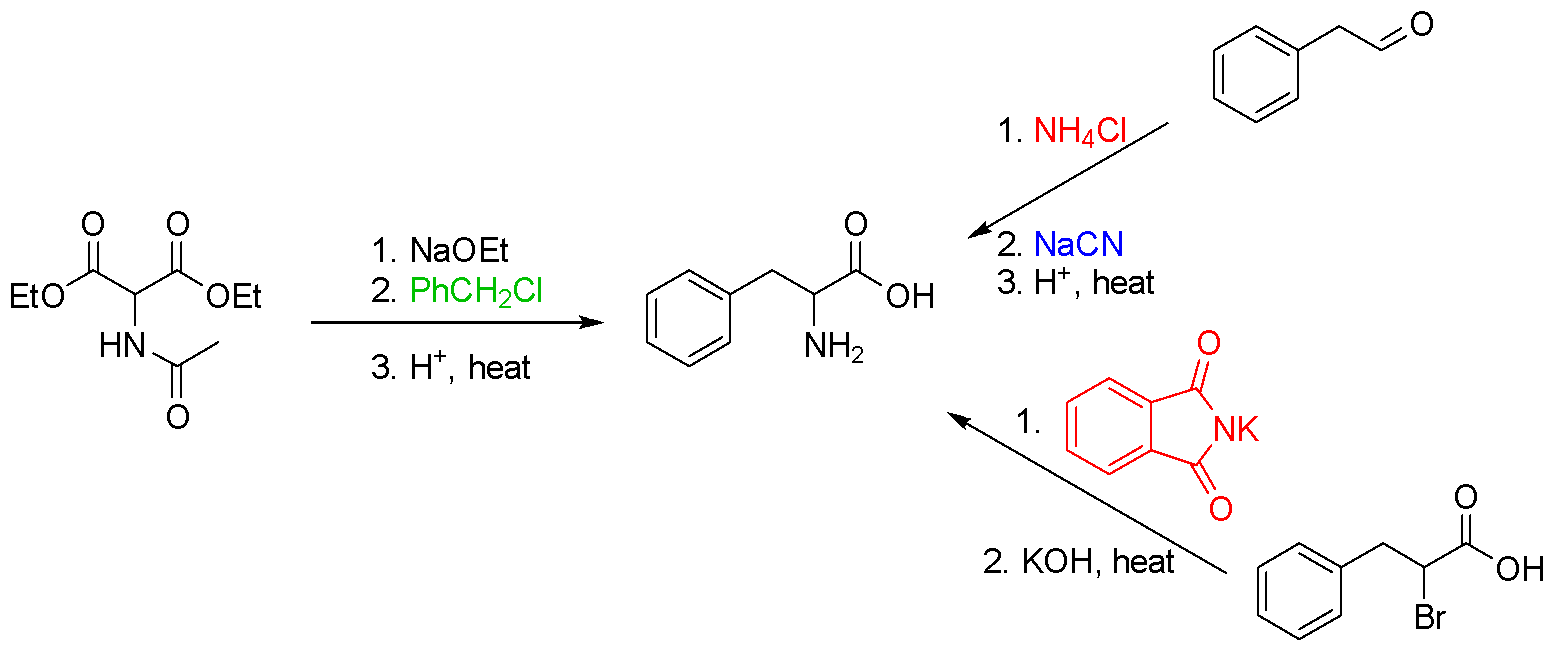
\includegraphics[width=0.9\textwidth]{Images/phenylalanine_synth.png}
  \caption{Phenylalanine synthetic scheme.}
  \label{fig:phenyl}
\end{figure}

In this work, we describe our initial studies directed at solving the challenging problem of computational retrosynthetic analysis. In particular, we develop a fully data driven seq2seq model that learns to perform the retrosynthetic reaction prediction subtask. For a given target molecule and a specified reaction type, the model predicts the most likely reactants that can react in the specified reaction type to produce the target molecule. The seq2seq model is trained end-to-end on a subset of experimental reactions with labelled reaction types \cite{schneider2016s} from an open source patent database \cite{lowe2012extraction}. We show that the trained seq2seq model performs comparably with a rule-based expert system baseline model on the relatively simple chemistry found in the patent dataset. 

\subsection{Approach}

\subsubsection{Problem definition}
Concretely, the retrosynthetic reaction prediction task is shown in Figure~\ref{fig:ret_problem_example}. Given an input SMILES that represents the target molecule and a specified reaction type, the model predicts the output SMILES which represents the likely reactants that can react in the specified reaction type to form the target molecule. 


\begin{figure}
  \centering
  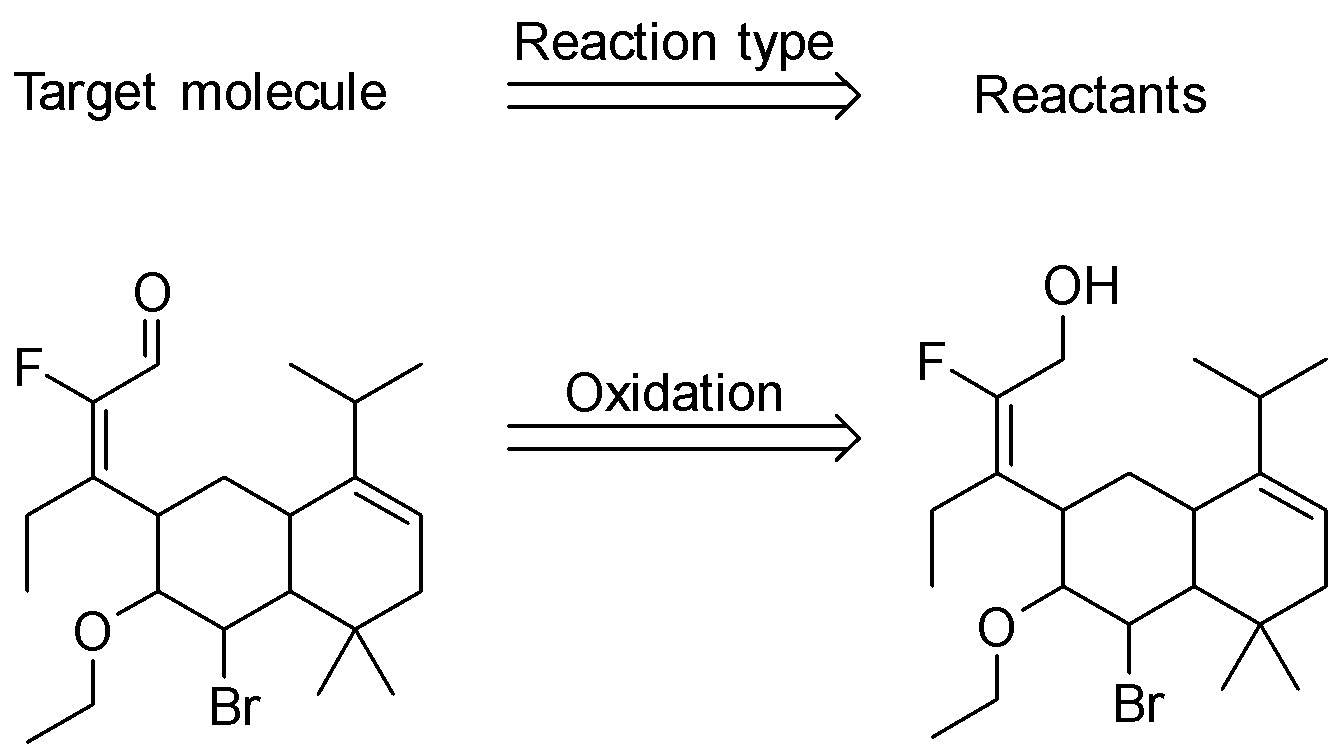
\includegraphics[width=0.9\textwidth]{Images/ret_problem_definition.png}
  \caption{Retrosynthetic reaction prediction task and an example of a possible retrosynthetic disconnection for a target molecule.}
  \label{fig:ret_problem_example}
\end{figure}

\subsubsection{Data preparation}

We use a filtered patent dataset, derived from an open source patent database \cite{lowe2012extraction}, which contains 50,000 atom-mapped reactions that have been classified into 10 broad reaction types \cite{schneider2016s} This filtered patent dataset was originally constructed to represent the typical reaction types found in the medicinal chemist’s toolkit. The reaction examples are further preprocessed to eliminate all reagents in order to only contain reactants and products \cite{schneider2016s}, and then canonicalized. We additionally process this dataset so that each reaction example contains a single product by splitting any reactions with multiple products into multiple single product reactions that contain the original reactants. Any resulting reaction examples with trivial products such as inorganic ions and solvent molecules are removed. Table \ref{fig:ret_table_1} shows the distribution of the 10 reaction classes in the final processed dataset. Finally, the dataset was split into training, validation and test datasets (8:1:1). 

\begin{figure}
  \centering
  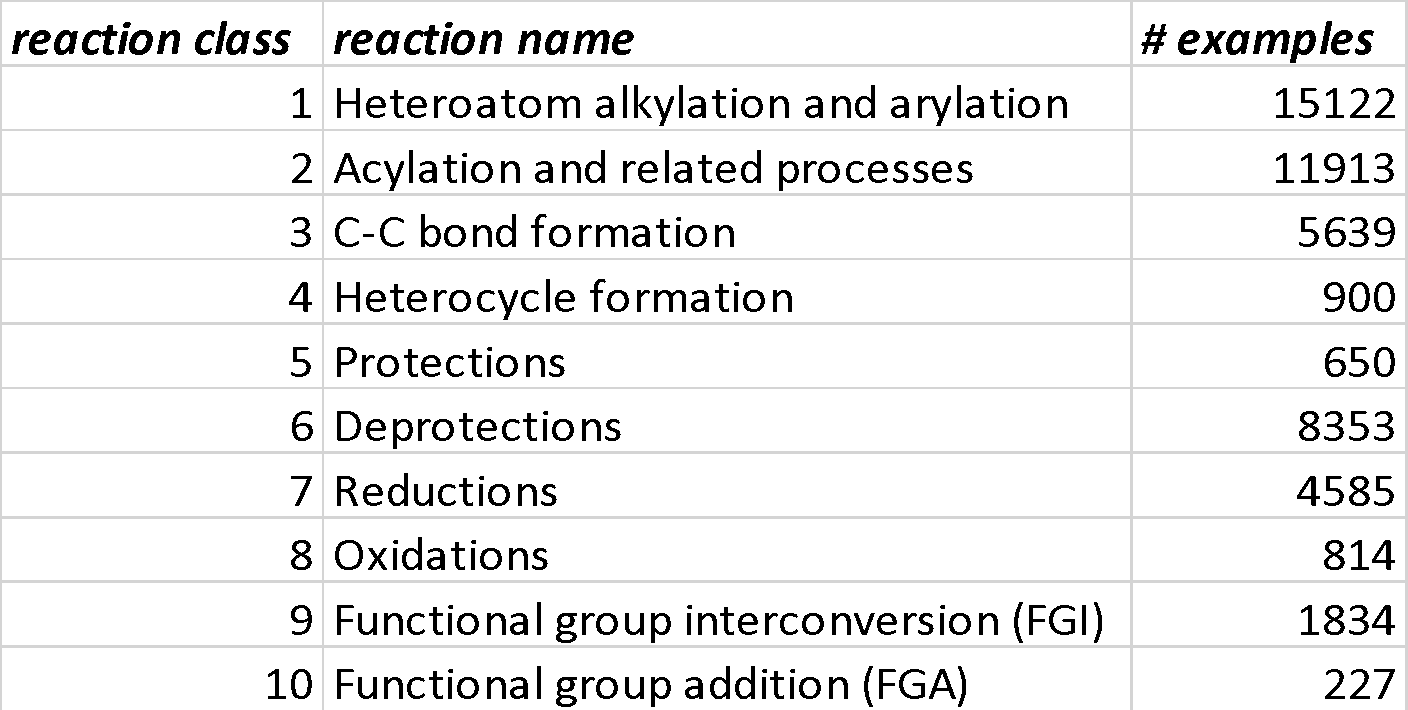
\includegraphics[width=0.9\textwidth]{Images/ret_table_1.png}
  \caption{Table: Distribution of major reaction classes within the processed reaction dataset.}
  \label{fig:ret_table_1}
\end{figure}

\subsubsection{Model}

\paragraph{Seq2seq model}

Neural sequence-to-sequence (seq2seq) models map one sequence to another, and have recently shown state of the art performance in many tasks such as machine translation \cite{bahdanau2014neural, sutskever2014sequence}. It is based on an encoder-decoder architecture that consists of two recurrent neural networks (RNN), and can include an attention mechanism that aligns the target tokens with the source tokens \cite{bahdanau2014neural}. Figure~\ref{fig:ret_seq2seq} shows a simple seq2seq encoder-decoder architecture for our retrosynthetic reaction prediction task.

\begin{figure}
  \centering
  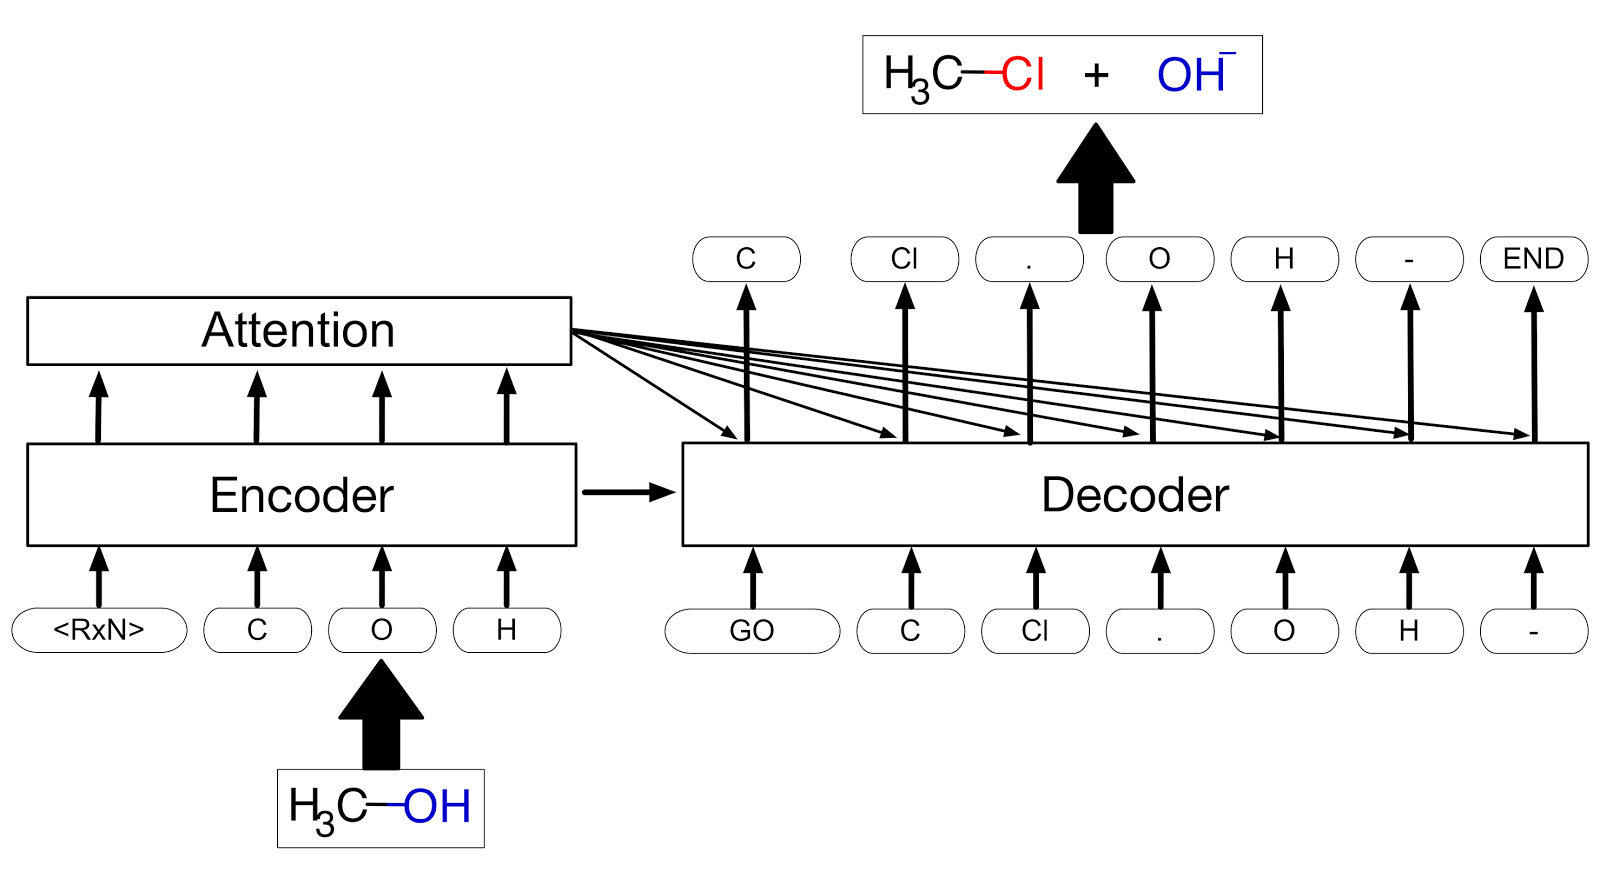
\includegraphics[width=0.9\textwidth]{Images/ret_seq2seq.png}
  \caption{seq2seq model architecture.}
  \label{fig:ret_seq2seq}
\end{figure}

We adapt the open source seq2seq library from Britz et al. \cite{britz2017massive} for our character-wise seq2seq model. The encoder-decoder architecture consists of Long Short Term Memory (LSTM) cells, which is a variant of RNN cells that more effectively learn long-range dependencies in the sequences \cite{hochreiter1997long}. More specifically, the seq2seq model consists of a bidirectional LSTM encoder and a LSTM decoder. Furthermore, an additive attention mechanism is used \cite{bahdanau2014neural}. The key hyperparameter settings of the seq2seq model are shown in Table S1.
The seq2seq model is trained on the training dataset with reaction atom-mapping removed. Each reaction example is split into a source sequence and target sequence. The source sequence consists of a sequence of characters that is derived from splitting the SMILES that correspond to the product into characters, with a reaction type token prepended to the sequence. The source sequence is reversed prior to feeding into the encoder. The target sequence consists of a sequence of characters that is derived from splitting the SMILES that correspond to the reactants into characters. The seq2seq model is evaluated every 4000 training steps on the validation dataset, and model training is stopped once the evaluation log perplexity starts to increase. 
Finally, the trained seq2seq model is evaluated on the test dataset with reaction atom-mapping removed. Each target molecule SMILES example from the test dataset is converted into an input sequence of characters, with a reaction type token prepended to the sequence, and reversed prior to feeding into the encoder. A beam search procedure is used for model inference. Figure~\ref{fig:ret_beam_search} depicts a partially completed beam search procedure with a beam width of 5 for an example input. For each source sequence input that represents the target molecule, the top N candidate output sequences ranked by overall sequence log probability at each time step during decoding are retained, where N is the width of the beam. The decoding is stopped once the lengths of the candidate sequences reach the maximum decode length of 140 characters. The candidate sequences that contain an end of sequence character are considered to be complete. On average, about 97\% of all beam search predicted candidate sequences are complete. These complete candidate sequences represent the reactant sets predicted by the seq2seq model for a particular target molecule, and they are ranked by the overall sequence log probabilities, which consists of the log probabilities of the individual characters in each complete candidate sequence. Additional beam search statistics and performance measures are shown in Table S2.

\begin{figure}
  \centering
  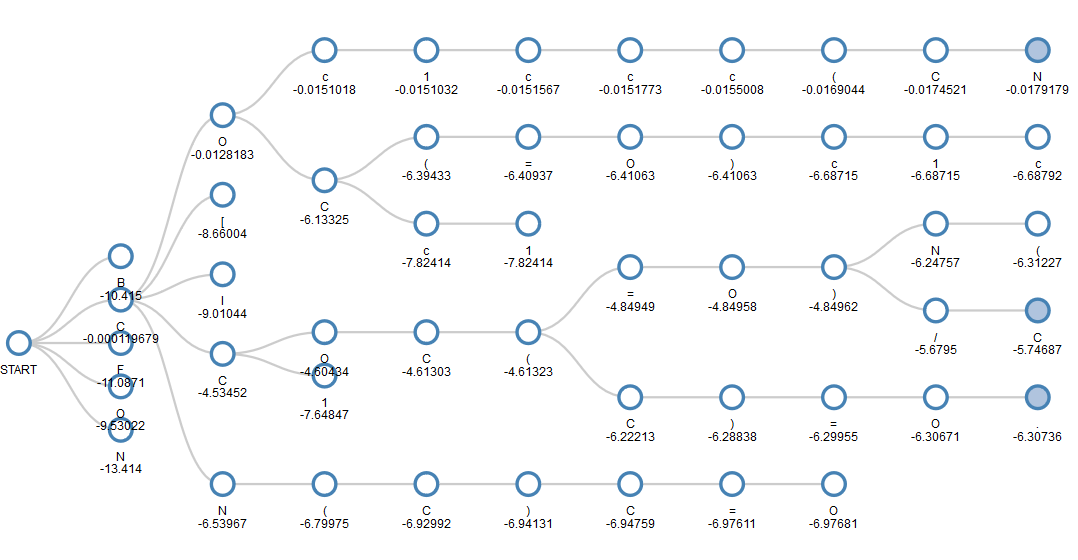
\includegraphics[width=0.9\textwidth]{Images/ret_beam_search.png}
  \caption{A partially completed beam search procedure with a beam width of 5 for an example input. Note that only the top 5 candidate sequences are retained at each time step. The visualization was produced using the seq2seq model library from Britz et al.51.}
  \label{fig:ret_beam_search}
\end{figure}

\paragraph{Baseline Model}
The baseline model is a rule-based expert system that applies retrosynthetic reaction rules of a specified reaction type to a target molecule to obtain the reactants. The reaction rules are automatically extracted from the training dataset. The rule extraction algorithm is adapted from Coley et al.’s implementation \cite{coley2017prediction}, which was based on the algorithms described by Law et al. \cite{law2009route} and Bogevig et al. \cite{bogevig2015route}. For each atom-mapped reaction example in the training dataset, the reaction centers are extracted by identifying changes in connectivity between product atoms and the corresponding reactant atoms. The reaction centers are expanded to include immediately neighboring atoms. A SMARTS string that describes the reaction core pattern is generated for the reactants and product, and combined to form a reaction SMARTS string that represents the retrosynthetic reaction rule. Each reaction rule is labelled with the reaction type of the corresponding reaction example that it was extracted from. Overall, 29272 valid rules were extracted from the training dataset, which represents a rule coverage of 73.1\% in the training dataset. A rule is defined to be valid if it is able to regenerate the product from the reactants and the reactants from the product in the reaction example from which the rule is extracted from. After filtering out duplicated rules, we end up with 2868 unique retrosynthetic reaction rules, defined by SMARTS strings. 
The rule-based expert system is evaluated on the test dataset. Each target molecule SMILES example from the test dataset is applied by all the rules of the particular reaction type. The resulting top N reactant sets obtained from the successful reaction rules are ranked by the number of occurrences of the corresponding rule of the target reaction class that were observed in the training dataset.
All scripts were written in Python (version 3.5), and RDKit (version 2016.09.04) \cite{landrumrdkit} was used for reaction preprocessing and rule extraction. The seq2seq model was built with TensorFlow (version 1.0.1) \cite{abadi2016tensorflow}.

\subsection{Results}

\subsubsection{Performance on the Test Dataset}

Table \ref{fig:ret_table2} shows the top-N accuracies of the rule-based expert system baseline and the seq2seq model on the test dataset. The top-N accuracy refers to the percentage of examples where the ground truth reactant set, which is the actual patent literature reported reactant set for the corresponding target molecule in the test dataset, was found within the top N predictions made by the model. By this metric, we observed that the seq2seq model performs comparably to the baseline model. Although the baseline model does not incorporate any NN component to perform candidate ranking, the performance of the baseline model becomes less sensitive to candidate ranking as N increases. The maximum accuracy of the baseline model, which is the percentage of examples where the ground truth reactant set was found in any of the predictions made by the baseline model, is 69.5\%. This represents the maximum possible test accuracy of the baseline model, as well as any deep learning approach that combines a NN component that performs candidate ranking with this rule-based expert system. The reason is that if no reaction rule exists that can produce the ground truth reactant set from the input molecule, then the NN component cannot rank it. The top-50 accuracy of the seq2seq model is higher than this maximum baseline accuracy. 


\begin{figure}
  \centering
  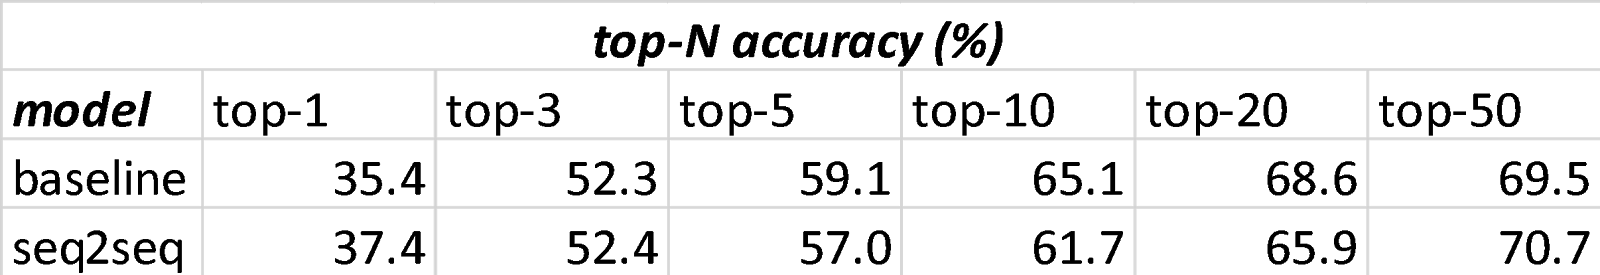
\includegraphics[width=0.9\textwidth]{Images/ret_table_2.png}
  \caption{Table: Comparison of top-N accuracies between the baseline and seq2seq models.}
  \label{fig:ret_table2}
\end{figure}

Some representative examples of correct seq2seq model predictions for each reaction class are shown in Figure~\ref{fig:ret_table2}. The examples are depicted in the retrosynthetic direction.

\begin{figure}
  \centering
  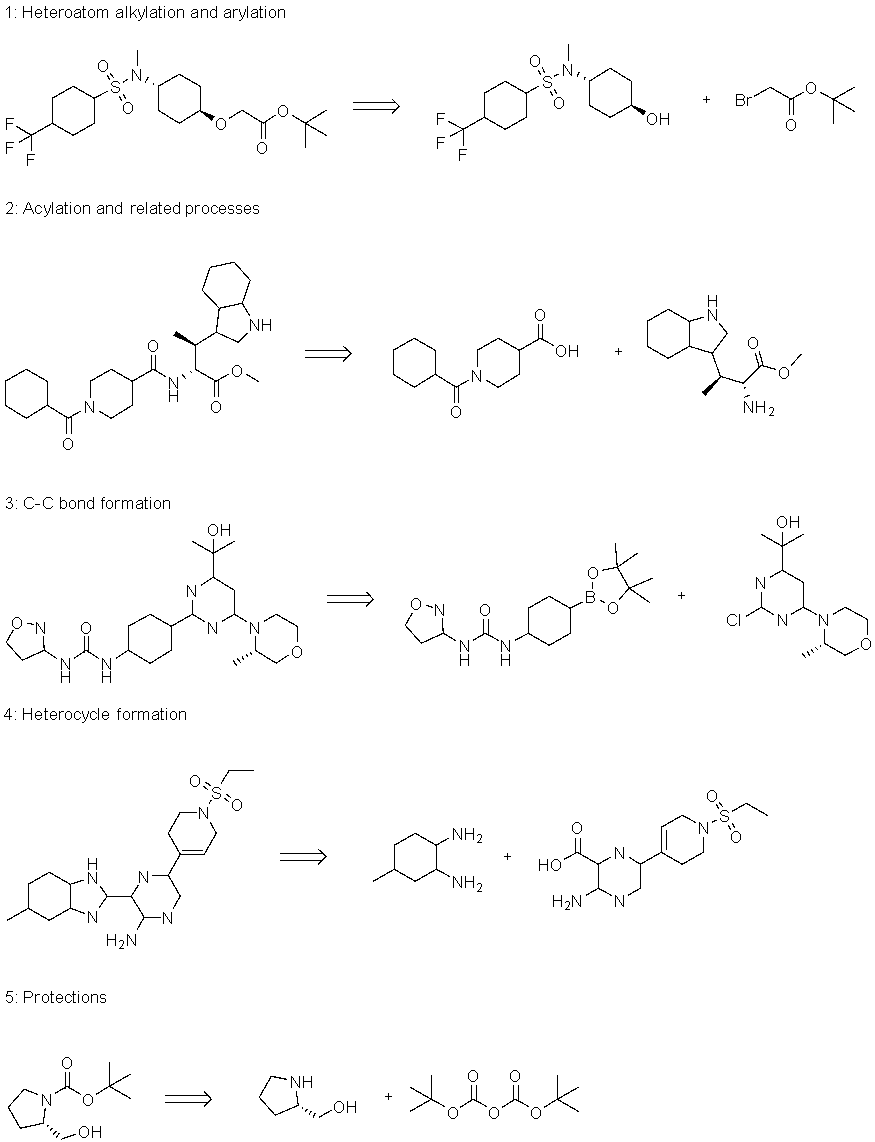
\includegraphics[width=0.9\textwidth]{Images/ret_seq2seq_correct.png}
  \caption{Representative examples of correct seq2seq model predictions for each reaction class.}
  \label{fig:ret_table2}
\end{figure}

\begin{figure}
  \centering
  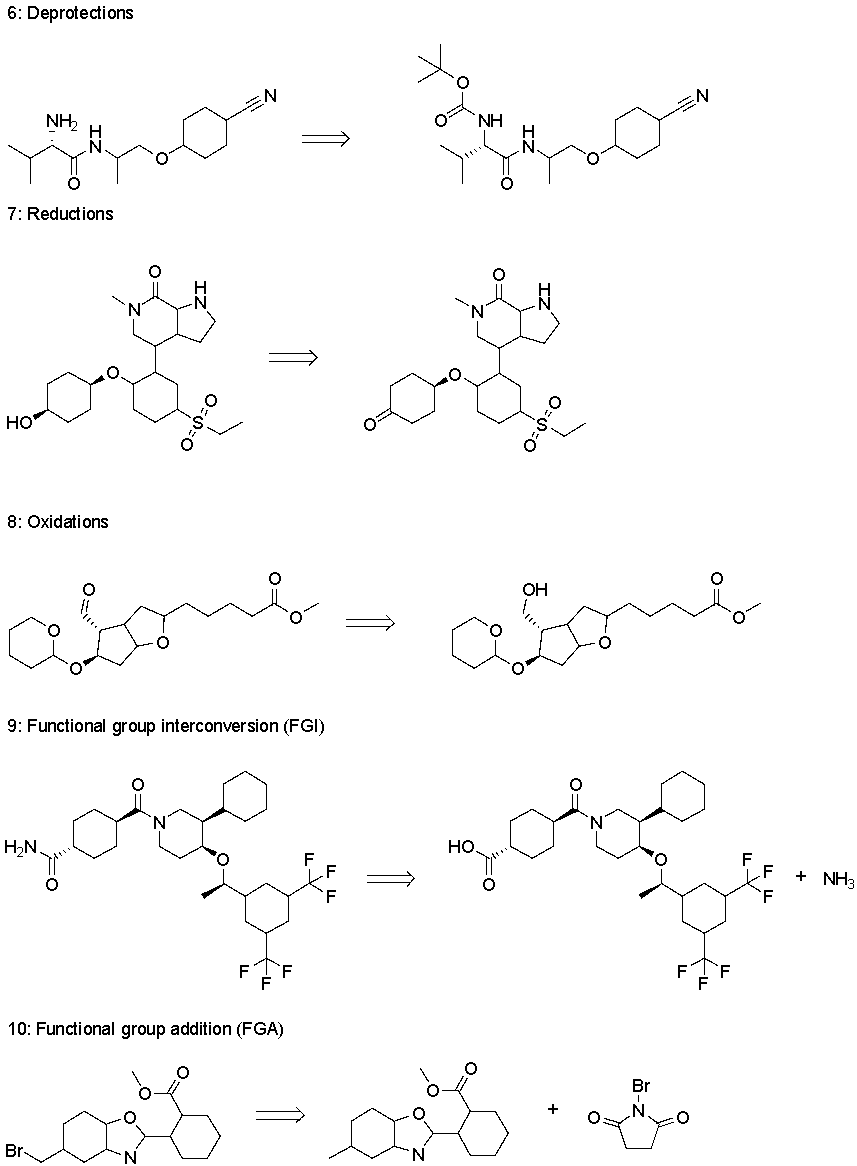
\includegraphics[width=0.9\textwidth]{Images/ret_seq2seq_correct_part_2.png}
  \caption{More Representative examples of correct seq2seq model predictions for each reaction class.}
  \label{fig:ret_table2}
\end{figure}

The detailed top-10 results for the baseline model and the seq2seq model broken down by the reaction classes is shown in Table \ref{fig:ret_table3}. The name of each reaction class is shown in Table \ref{fig:ret_table_1}.

\begin{figure}
  \centering
  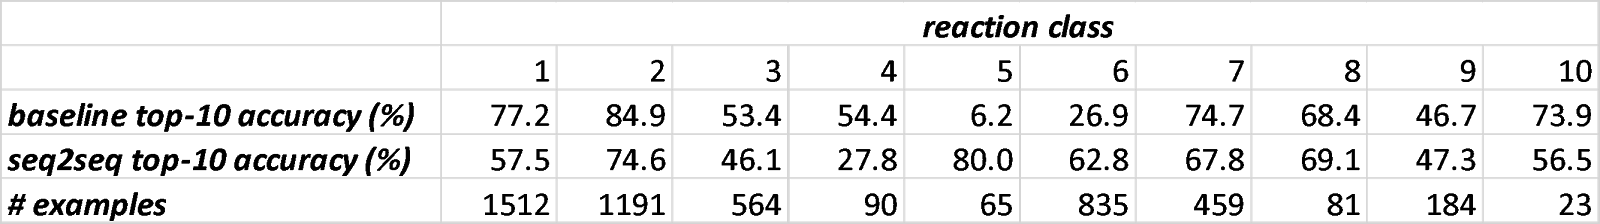
\includegraphics[width=0.9\textwidth]{Images/ret_table_3.png}
  \caption{Table: Breakdown of the top-10 accuracy of the baseline and seq2seq models by reaction class.}
  \label{fig:ret_table3}
\end{figure}

The baseline model performs significantly better in reaction class 1 (heteroatom alkylation and arylation) and reaction class 2 (acylation and related processes). The common feature of these reaction classes is that the reactions are possible with many possible functional groups at the reaction site. For example, in Figure 5, the acylation reaction between a carboxylic acid and an amine would also be possible with another carbonyl compound that has a suitable leaving group, such as an acyl chloride. Additionally, the target molecules in the dataset for these reaction classes often have multiple possible reaction sites. The knowledge base in the baseline model contains reaction rules for each of the possible functional groups that were present in the reaction examples from the training dataset. Therefore, the baseline model is able to easily enumerate reactant sets that span most of the possible functional group and reaction site combinations. On the other hand, the seq2seq model currently predicts only a few valid reactant sets that contain different possible functional group and reaction site combinations. As a result, the particular ground truth reactant set is more likely to be found in the predicted reactant sets from the baseline model. 

The baseline model also performs significantly better in reaction class 4 (heterocycle formation). The key feature of this reaction class is the formation of cyclic and aromatic structures, which results in a large difference between the reactant set SMILES string and the target molecule SMILES string. Also, there is a relatively small number of reaction examples in the training dataset for this reaction class. Overall, these two factors cause the seq2seq model to make a lot of grammatical mistakes in the SMILES predictions. 

The seq2seq model performs significantly better in reaction class 5 (protections) and reaction class 6 (deprotections). The common feature of reaction classes 5 and 6 is that the reactants have large leaving groups that are not included in the product side. As a result, the very general rules in the baseline model, which only contain the immediate neighborhood of the reaction centers, do not capture the identities of the leaving groups. Conversely, the seq2seq model captures the global molecular environment of all the reaction species and is able to predict the leaving groups correctly. 

\paragraph{Error analysis of the seq2seq model}

The seq2seq model makes three kinds of prediction errors:

\begin{figure}
  \centering
  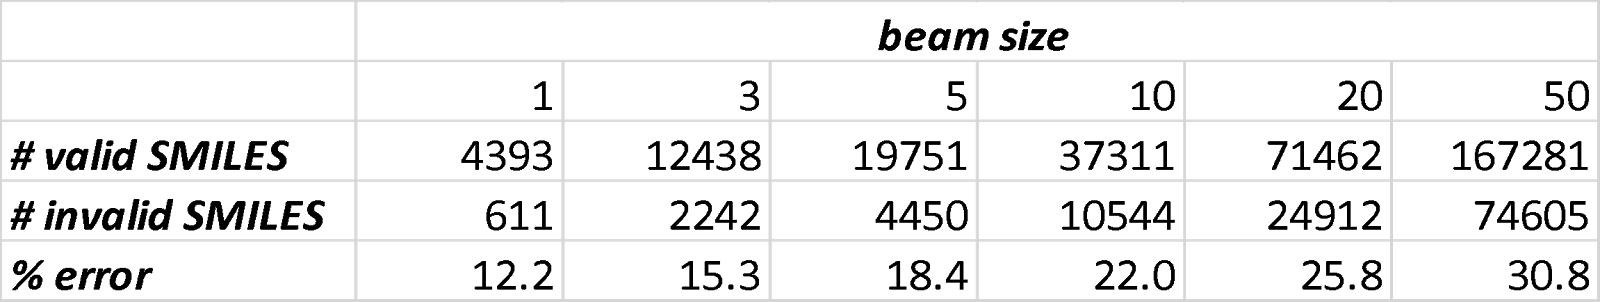
\includegraphics[width=0.9\textwidth]{Images/ret_table_4.png}
  \caption{Breakdown of the grammatically invalid SMILES error for different beam sizes.}
  \label{fig:ret_table4}
\end{figure}

\begin{figure}
  \centering
  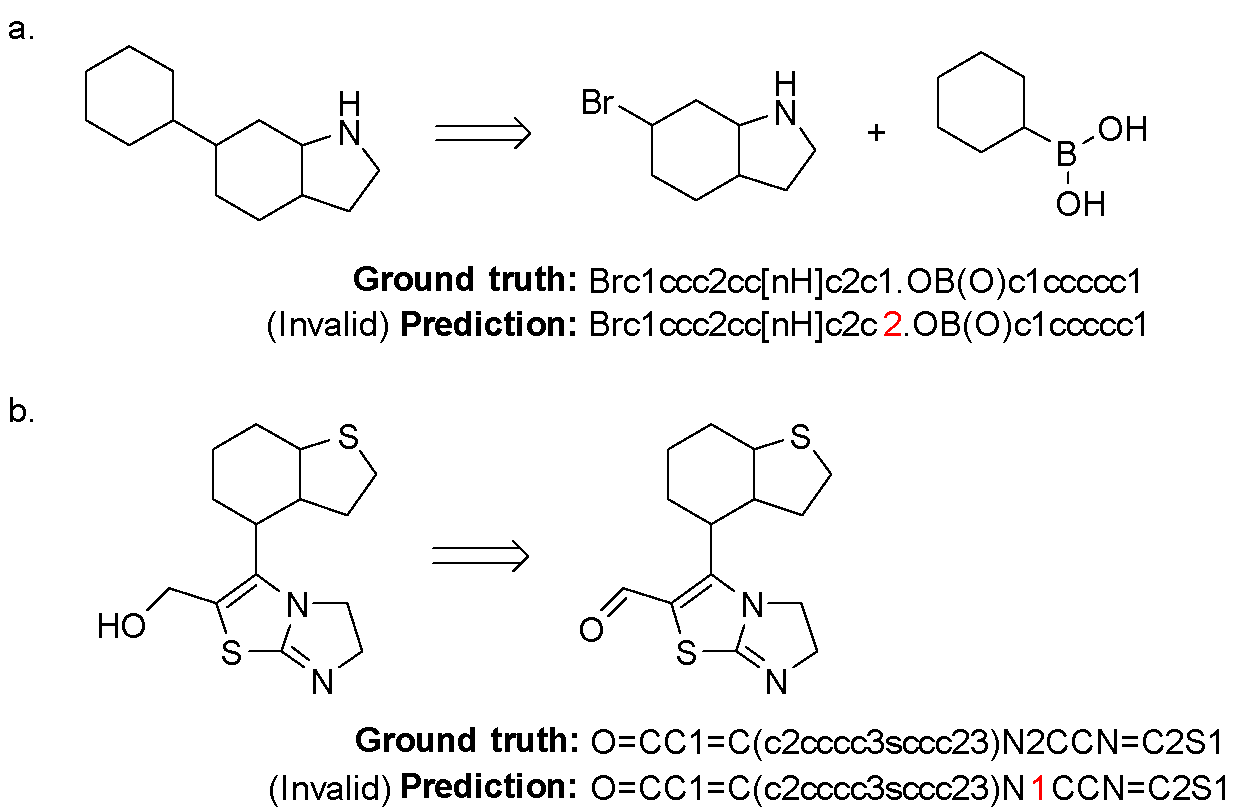
\includegraphics[width=0.9\textwidth]{Images/ret_seq2seq_grammer_invalid.png}
  \caption{Examples of reactant SMILES that are grammatically invalid: (a) reaction class 3 (C-C bond formation); (b) reaction class 7 (Reductions).}
  \label{fig:ret_table2}
\end{figure}

\begin{figure}
  \centering
  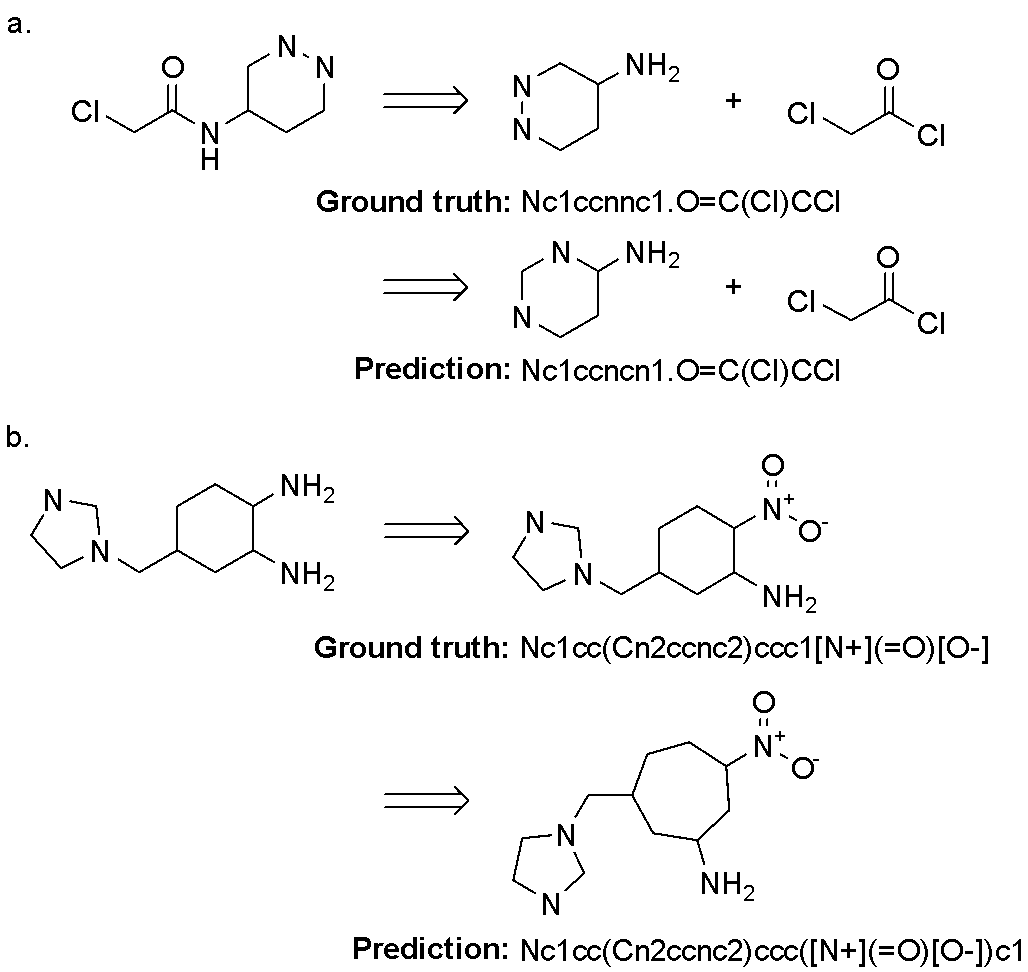
\includegraphics[width=0.9\textwidth]{Images/ret_seq2seq_implausible.png}
  \caption{Examples of reactant SMILES that are grammatically valid, but the overall reaction is chemically implausible: (a) reaction class 2 (Acylation and related processes); (b) reaction class 7 (Reductions).}
  \label{fig:ret_table2}
\end{figure}

\begin{figure}
  \centering
  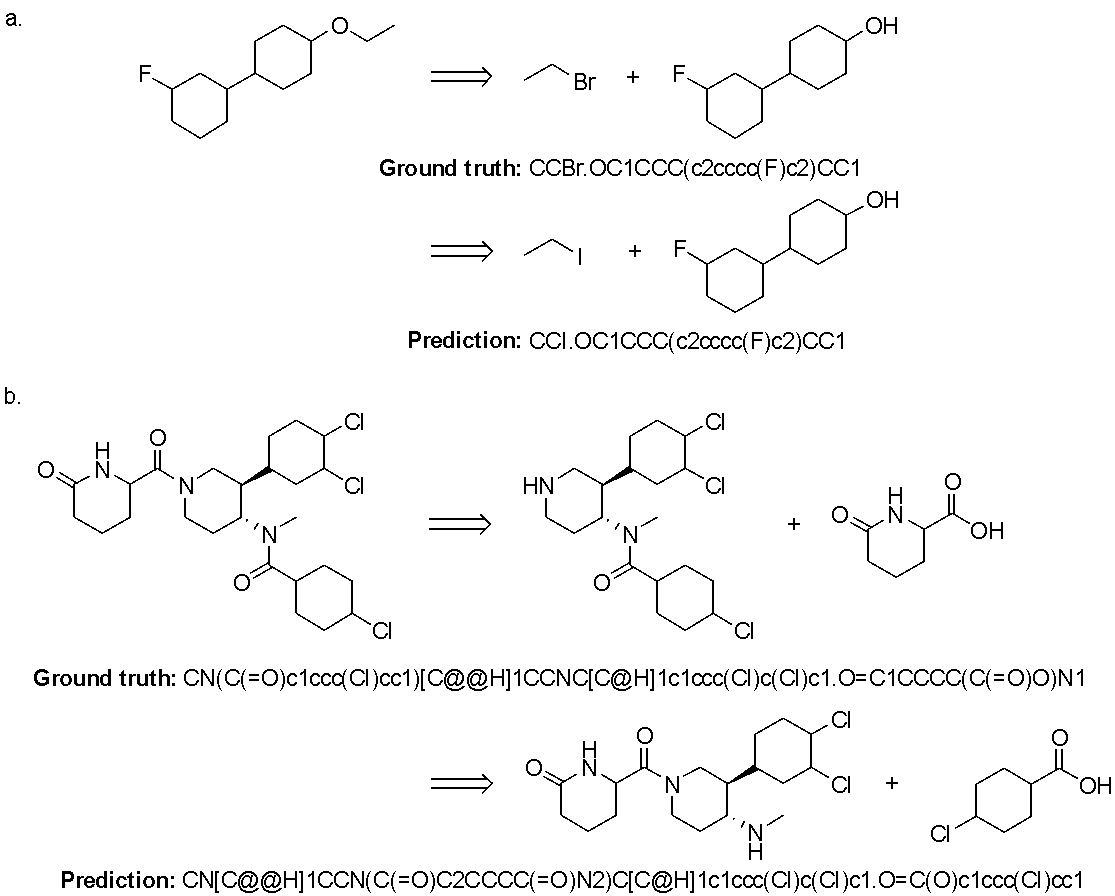
\includegraphics[width=0.9\textwidth]{Images/ret_seq2seq_plausible.png}
  \caption{Examples of reactant SMILES that are grammatically valid and the overall reaction is chemically plausible: (a) reaction class 1 (Oxidations); (b) reaction class 2 (Acylation and related processes)}
  \label{fig:ret_table2}
\end{figure}

\begin{enumerate}
    \item The predicted reactant SMILES is grammatically invalid. This is a result of the SMILES text representation of the molecules, which is fragile because single character alterations can completely invalidate the SMILES. Since the seq2seq decoder does not explicitly understand the grammar that underlie the SMILES representation, and also formulates predictions one character at a time, it is likely that some of the predicted reactant SMILES are invalid. Table \ref{fig:ret_table4} shows a breakdown of this type of error and Figure 6 shows examples of this type of error.
    \item The predicted reactant SMILES is grammatically valid, but the overall reaction is not chemically plausible. This is a typical error in which the predicted reactant set cannot react in the specified reaction type to produce the target molecule. Many of these errors can also be attributed to the fragile SMILES text representation because small alterations in the SMILES can result in very large differences in the resulting molecule. Figure 7 shows examples of this type of error.
    \item The predicted reactant SMILES is grammatically valid and the overall reaction is chemically plausible. Although the predicted reactant set does not match the ground truth reactant set, the predicted reactant set is likely to react in the specified reaction type to produce the target molecule. One reason for this type of error is the possibility of multiple possible functional groups combinations or reactants that can react in the same reaction type to form the target molecule. Another reason is the presence of multiple reaction sites in the target molecule that can be disconnected retrosynthetically, so multiple possible reactant sets are chemically plausible. Figure 8 shows examples of this type of error.
\end{enumerate}

\paragraph{Ranking of the seq2seq model predictions}

The ranked predictions from the beam search decoding procedure of seq2seq model correspond well to chemical reactivity. For the top-10 predictions with both the baseline and seq2seq models, Figure 9 depicts a histogram that shows the counts of the highest rank that is assigned to the prediction which matches the ground truth for each example in the test dataset. Overall, the higher the rank of the prediction, the more likely that the prediction corresponds to the ground truth. The distribution for the seq2seq model is much more skewed towards the highest ranks compared to the baseline model, which naively ranks by the number of occurrences of the rules that was observed in the training dataset. 


\begin{figure}
  \centering
  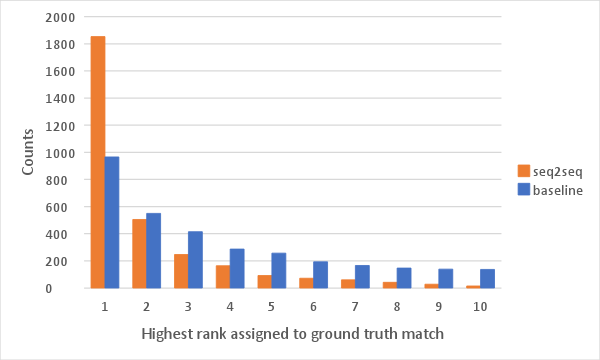
\includegraphics[width=0.9\textwidth]{Images/ret_histograph.png}
  \caption{Histogram of the highest rank assigned to the ground truth match in the top-10 predictions of the seq2seq and baseline models for each example. Note that the relative total counts across all the ranks for the seq2seq and baseline models is proportional to their relative top-10 accuracies shown in the table.}
  \label{fig:ret_table2}
\end{figure}

\paragraph{Analysis of the seq2seq model attention weights}

Figures S1-S10 show the attention weights between characters in the input sequence, which represent the target molecule and specified reaction type, and characters in the output sequence, which represent the predicted reactants, for representative examples of correct seq2seq model predictions in each reaction class. The attention weights provide information on which characters in the input sequence were considered to be more important when a particular character in the output sequence was generated. Generally, we see strong weights that trend diagonally, which monotonically align molecular substructures that are shared between the input and output. Additionally, we see that the input reaction type token generally has high weights with characters in the output sequence that correspond to the neighborhood of the reaction centers.

\subsection{Discussion}

\subsubsection{Comparison between the seq2seq and rule-based baseline model}

The seq2seq model performs comparably to the rule-based baseline model on the processed patent dataset, although the models perform differently for certain reaction types. Importantly, the seq2seq model has some significant advantages compared to the baseline model, and by extension to the deep learning based approaches that combine a rule-based expert system with a NN model for candidate ranking.

Firstly, the seq2seq model can be trained in a fully end-to-end manner directly from the training dataset. The seq2seq model both implicitly learns the chemical rules, and performs candidate ranking via the beam search decoding procedure. Conversely, the typical deep learning approach to reaction prediction combines a rule-based expert system component with a NN model component for candidate ranking, where the individual components need to be independently set up and trained. Also, any rule-based expert system that automatically extracts reaction rules from the reaction dataset depend heavily on accurate atom-mapping to describe the correspondence between the reactant and product atoms, which is itself a non-trivial problem \cite{chen2013automatic}. The seq2seq model does not require atom-mapped reaction examples for training. 

Secondly, the seq2seq model scales better to larger training datasets. The efficiency of rule-based expert systems depends on the number of rules in the knowledge base, which is an issue because the size of the knowledge base generally increases as the size of the training dataset increases. For the baseline model, as well as any deep learning approaches that use a rule-based expert system and a NN component to rank the likelihood of each predicted molecular species for a given example \cite{coley2017prediction}, the inference cost directly depends on the size of the knowledge base since every rule in the knowledge base must be exhaustively applied. On the other hand, the inference cost of a particular seq2seq model is independent of the size of the training dataset and depends primarily on the width of the beam search decoding procedure. For deep learning approaches that use a rule-based expert system and a NN component to rank the applicability of each rule in the knowledge base for a given example \cite{segler2017neural, wei2016neural}, a previous study showed that the classification accuracy decreases as the size of the knowledge base increases for a specific training dataset size, likely because the number of reaction rules that needs to be ranked in the multiclass classification problem also increases \cite{segler2017neural}. Overall, as training dataset size increases, the increasing NN accuracy from more training examples is partially offset by the negative effect on accuracy from the increased number of reaction rules to classify. In order to reduce the number of rules in the knowledge base, previous studies \cite{segler2017neural, coley2017prediction} removed rare reaction rules that occurred fewer times than a specified threshold. A side effect of this is a reduced rule coverage over the reaction examples, especially for rare reactions types. 

Thirdly, the seq2seq model incorporates information about the global molecular environment since the model learns from the complete SMILES for both the reactants and the target molecule in each reaction example. Also, the complete input target molecule SMILES is used to make predictions. However, the baseline model focuses only on the local molecular environment because the automatically extracted reaction rules in the knowledge base only incorporate the immediately neighboring atoms around the reaction centers. This results in an important issue with rule-based expert systems when performing the retrosynthetic reaction prediction task. In particular, the reaction examples in the dataset are processed into the form depicted in Figure 2, where each reaction consists of a single target molecule and one or more reactants. In all cases, every atom in the target molecule is atom-mapped and can be linked to reactant atoms. Unfortunately, the inverse is not true because for most reaction classes, not all atoms in the reactants are atom-mapped. These unmapped reactant atoms are the leaving groups which are not incorporated into the target molecule structure in the forward reaction. The issue arises when the leaving groups are large, which occurs commonly in reaction classes 5 (protections) and 6 (deprotections). If very general reaction rules are extracted that only contain the immediate neighborhood of the reaction centers, they will not fully capture the identities of the leaving groups. As a result, for these reaction classes that involve large leaving groups, the rules do not have sufficient information to reproduce the reactants from the target molecule. One solution would be to extract more specific rules that contains a larger neighborhood around the reaction centers in order to capture the identities of the leaving groups. However, the disadvantage with more specific rules is that they are less generalizable to new examples in the test dataset. Ultimately, there is a tradeoff between defining very general reaction rules and defining very specific reaction rules, which is challenging without manual intervention. Furthermore, a direct benefit of the seq2seq model incorporating the global molecular environment is that the model naturally accounts for stereochemistry. On the other hand, in order for deep learning approaches that combine a rule-based expert system with a NN model component to account for stereochemistry, both the reaction rules in the knowledge base and the descriptors that are used in the NN model must incorporate stereochemistry. Existing algorithms that automatically extract reaction rules do not fully address the issue of stereochemistry. 

\subsubsection{Molecular representations}

The seq2seq model maps one sequence to another, which restricts us to representing molecules using text sequences. In this study, we predominantly focused on the SMILES text representation because it has characteristics that make it particularly attractive as a text representation for molecules in a product to reactant sequence-to-sequence mapping task. Generally, when a reaction is expressed in a SMILES representation, there are many subsequences that are shared between the reactant and product SMILES strings. The SMILES representation reflects the fact that most reactions modify a particular reaction center, while keeping other parts of the molecule the same. The presence of shared subsequences between the input and output sequences makes the sequence-to-sequence mapping task relatively easier because the input and output sequences are similar. In comparison, our preliminary experiments using the InChI text representation for molecules in the seq2seq model resulted in worse performance when compared to using SMILES. This outcome is likely because InChI has a more complicated hierarchical syntax, which involves arithmetic to obtain the atom connectivity, and also there are fewer shared subsequences between the reactant and product InChI strings in a reaction. The weaker performance of InChI compared with SMILES when applied in an model that decodes text sequences is also in agreement with the observations of Gómez-Bombarelli et al. \cite{gomez2016automatic}  in their autoencoder architecture for generating molecular structures. Nonetheless, our results have shown that a key weakness with representing molecules using text sequences is the fragility of the representation, since very small changes in the text sequence can result in a very large change in the resulting molecular structure. A more natural way to represent molecules is to directly use graph representations, and our future work will explore model architectures that can take advantage of this feature.

\subsection{Conclusion}

Overall, we have created a data driven neural sequence-to-sequence model to solve the retrosynthetic reaction prediction task, which is a critical task in computational retrosynthetic analysis. While the current implementation of the seq2seq model performs comparably to the rule-based expert system baseline, the seq2seq model has fundamental advantages over rule-based expert systems and over any deep learning approach that depends on a rule-based expert system component. The seq2seq model can be trained in an end-to-end manner, scales more efficiently to larger datasets, and naturally incorporates the global molecular environments of the reaction species. We believe that there exists significant room for improvement over the current relatively unoptimized seq2seq model, so further work is likely to lead to greater prediction accuracies. 

In following work, we will seek to increase the accuracy of the seq2seq model by exploring architectural variants and by exploring new datasets. Additionally, since the seq2seq model is a very general architecture for mapping input sequences to output sequences, we could include reaction conditions and yields during training in order to predict reaction conditions and yields alongside the reactants during the decoding procedure. Furthermore, an interesting extension to the seq2seq models would be to use one-shot techniques \cite{vinyals2016matching, santoro2016one, altae2017low} to allow our retrosynthetic reaction prediction models to make reasonable predictions for reaction classes where only a few example reactions are available for training. We envision that our seq2seq model and its future variants would act as the single step reaction prediction module in a multistep retrosynthetic analysis tool, whereby a search procedure recursively deconvolutes the target molecule using the chemistry learned by the seq2seq model until simple or commercially available precursor molecules are obtained.

We believe that the approach and model architecture described in this work is an important early step towards solving the computational retrosynthetic analysis problem. Although the chemical complexity of the reactions and molecules explored in this work are intentionally simple to facilitate analysis and thus are quite far away from what is typically faced by mainstream synthetic chemists today, we strongly believe that the future evolution of this approach could bridge this gap and result in tools that can become broadly useful for the expert chemist and also more broadly for those less skilled in the science.

\subsection{Acknowledgments}

We thank Franklin Lee for critical reading and feedback on the manuscript. 
B.L. is supported by the NIH (U19 AI109662). B.R. is supported by the Fannie and John Hertz Foundation. S.H. is supported by a Postdoctoral Fellowship, PF-15-007-01-CDD from the American Cancer Society.
The Pande Group is broadly supported by grants from the NIH (R01 GM062868 and U19 AI109662) as well as gift funds and contributions from Folding@home donors. This research was also supported by the National Science Foundation (P.A.W.: CHE1265956).

We acknowledge the generous support of Dr. Anders G. Frøseth for our work on machine learning.

\subsection{Declarations}

VSP is a consultant and SAB member of Schrodinger, LLC and Globavir, sits on the Board of Directors of Apeel Inc, Freenome Inc, Omada Health, Patient Ping, Rigetti Computing, and is a General Partner at Andreessen Horowitz

%\clearpage
%\section{Is Multitask Deep Learning Practical for Pharma?}

\subsection{Abstract}
Multitask deep learning has emerged as a powerful tool for computational drug discovery. However, despite a number of preliminary studies, multitask deep networks have yet to be widely deployed in the pharmaceutical and biotech industries. This lack of acceptance stems from both software difficulties and from lack of understanding of the robustness of multitask deep networks. Our work aims to resolve both of these barriers to adoption. We introduce a high-quality open-source implementation of multitask deep networks as part of the DeepChem open-source platform. Our implementation enables simple python scripts to construct, fit, and evaluate sophisticated deep models. We use our implementation to analyze the performance of multitask deep networks and related deep models on four collections of pharmaceutical data (three of which have not previously been analyzed in the literature). We split these datasets into train/valid/test using time and neighbor-split to test multitask deep-learning performance under challenging conditions. Our results demonstrate that multitask deep networks are surprisingly robust and can offer strong improvement over random forests. Our analysis and open-source implementation in DeepChem provide an argument that multitask deep-networks are ready for widespread use in commercial drug discovery. 


\subsection{Introduction}
Deep learning has had unprecedented impact on computer science and technology over the last five years. The advent of sophisticated deep models has enabled the construction of powerful visual, speech, and natural language understanding systems \cite{lecun2015deep}. Over the past few years, deep learning has begun to influence drug discovery. In 2012, MSD (Merck \& Co., Inc., Kenilworth, NJ USA) hosted a Kaggle contest to measure the ability of data-science to improve predictive accuracies of quantitative structure-activity relationship (QSAR) methods. The winning entry used multitask deep networks (ensembled with other machine-learning techniques) to achieve a 15\% relative improvement over the baseline \cite{DahlKaggle}. In follow-up work, MSD demonstrated that strong improvements could be 
achieved on the Kaggle datasets using a single deep learning architecture, without constructing ensemble models \cite{ma2015deep}. In parallel, other research has demonstrated that large scale multitask deep networks can yield strong improvements over singletask models on public datasets with hundreds of tasks, extending MSD's work with smaller dataset collections \cite{ramsundar2015massively,unterthiner2014deep}. Similarly, recent work from Vertex demonstrates that multitask deep networks can offer improvements over simpler methods for modeling ADMET (absorption, distribution, metabolism, excretion, and toxicity) datasets \cite{kearnes2016modeling}. 

However, despite significant preliminary research, deep multitask networks have not succeeded in achieving broad adoption in the pharmaceutical and biotechnology industries. Transforming a machine-learning based research prototype into a production system can present
many challenges. For example, the winning entry for Netflix's million dollar recommendation challenge was not actually deployed in Netflix's production system due to engineering costs \cite{netflixNever}. Parts of the solution (singular value decompositions and restricted Boltzmann machines) were deployed, but shifting customer requirements rendered the full solution too unwieldy for broad implementation \cite{netflixBlog}.

Similar challenges may well be slowing the broad adoption of multitask deep networks in the pharmaceutical industry. Drug discovery companies often don't have strong software development teams, and creating a high-quality multitask deep network implementation is a formidable software engineering challenge. Each piece of research cited above uses an independent multitask implementation. While a research team may be able to create custom deep-learning implementations, such feats remain challenging for industrial teams. Until recently, a similar situation held more broadly within the deep learning community. While research teams could implement deep-learning systems, industrial users often stayed away due to the engineering challenges. However, this situation changed dramatically with the advent of sophisticated open source deep learning frameworks such as Tensorflow, Theano, and Keras \cite{abadi2016tensorflow,bastien2012theano,chollet2015keras}. These platforms offer convenient software primitives for building sophisticated deep architectures with low-overhead. As a result, the adoption of deep-learning techniques by the software industry has increased accordingly.

While deep learning systems offer powerful conveniences for users, the native
%comment MT: replace raw with native
packages are not well-suited to handle chemical datasets. Data loading procedures don't support common chemical formats such as SMILES strings \cite{weininger1988smiles} or provide for data-splits based on chemical scaffolds \cite{bemis1996properties}. The DeepChem library developed at Stanford provides a wrapper around Tensorflow that understands and facilitates the processing of chemical datasets \cite{deepchem}. DeepChem has been used for both application projects (modeling inhibitor design for BACE-1 \cite{subramanian2016computational}) and for algorithmic development (of novel one-shot deep-learning techniques for drug discovery \cite{altae2017low}).

In this work, we introduce a high-quality multitask deep network implementation to DeepChem. We use this implementation to construct multitask models on four broad collections of pharmaceutical data. We start by using DeepChem's implementation to reproduce results on the Kaggle collection explored by MSD previously. We then construct multitask deep models on the Factors, Kinase, and UV dataset collections from MSD (previously not analyzed in the literature). We aim to investigate whether multitask deep-learning is a robust tool; one that provides strong results across broad collections of pharmaceutical data.

We focus our analysis on gauging whether multitask networks provide consistent improvements over random-forest baselines. In particular, we aim to answer the question of whether deep networks can replace random-forest models without causing significant failures on a subset of predictive models. Furthermore, due to the ease of implementing new deep-learning architectures in DeepChem, we test the performances of two alternate deep learning architectures on these datasets. Google's Deepmind recently proposed progressive neural networks as a suitable architecture for solving sequences of challenging learning tasks \cite{rusu2016progressive} while leveraging transfer learning and avoiding learning failures. Progressive networks require an ordering of learning tasks (often unnatural in a drug-discovery setting with a collection of assays), so we also consider a variant bypass architecture halfway between multitask networks and progressive networks. Our analysis reveals that while these alternative architectures offer reasonable results, the simple multitask deep architecture currently remains the most robust deep architecture for QSAR datasets. On average, multitask deep networks offer performance boosts over random forest methods, but the improvements are not yet across the board.

To encourage adoption of multitask deep-learning methods, we open source all modeling code and datasets for the Kaggle, Factors, Kinase, and UV dataset collections as part of the DeepChem example suite. We hope that this example code and data will facilitate broader adoption of multitask deep-learning techniques for commercial drug discovery.

\subsection{Multitask Deep Learning with DeepChem}
\begin{figure}
  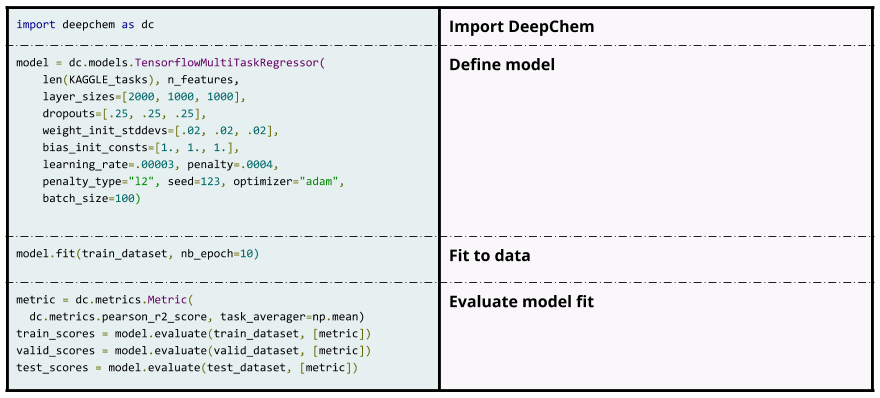
\includegraphics[width=\textwidth]{Images/deepchem_code.png}
  \caption{Example code for defining, training, and evaluating multitask deep networks for the Kaggle dataset with DeepChem. Code example is nearly complete, except for loading code. Full code for building networks on Kaggle datasets is available online}
  \label{fig:code}
\end{figure}

DeepChem offers a python API for constructing multitask deep-learning models. The API is object-oriented and modeled on the interfaces for popular machine-learning packages such as Scikit-Learn \cite{pedregosa2011scikit} and Keras \cite{chollet2015keras}. As part of this work, we contribute a high quality multitask deep network implementation to DeepChem.
%comment MT: DeepChem
Users can build, train, and evaluate multitask deep networks with simple python scripts.

Figure~\ref{fig:code} provides an (almost complete) code sample for using the multitask deep learning API in DeepChem to build a model for the Kaggle data collection. Users can specify model hyperparameters in the constructor for the multitask deep network. Figure~\ref{fig:code} demonstrates how a three hidden layer deep network, with dropout \cite{srivastava2014dropout} and $L^2$ regularization can be specified. Calling the \texttt{fit()} method fits the model using the ADAM optimization algorithm \cite{kingma2014adam} for 10 epochs over the training dataset. Note that code in 
%comment MT: add 'code in'
Figure~\ref{fig:code} has a \texttt{seed} flag for deep models. This flag allows multitask deep networks to be constructed in DeepChem with fixed random seed. Otherwise, model performance may vary on the order of a few percent due to random initialization choice, making debugging and model optimization challenging. Calling the \texttt{evaluate()} method allows users to evaluate the model using the squared Pearson correlation coefficient.

The full example for the Kaggle dataset is only slightly longer and has been open-sourced as part of the DeepChem example suite.

\subsection{Datasets}

\subsubsection{Data Description}
Modeling was performed on four collections of assays from MSD (see Table~\ref{tab:datasets} for details). The Kaggle collection is a collection of 15 of enzymatic inhibition and ADME/Tox datasets \cite{ma2015deep} with about 100,000
unique compounds. Not every compound in the Kaggle collection is tested against every assay. The Factors collection measures about 1500 of MSD's in-house compounds for IC50 of inhibition on 12 serine proteases, some of which are blood-clotting factors. The Kinase colection contains about 2500 in-house compounds measured for IC50 of inhibition on 99 protein kinases, carried out by a contract research partner. The UV collection tests 10,000
compounds on 190 absorption wavelengths, between 210 and 400 nanometers.

Pre-computed AP,DP (atom-pair, donor-pair) descriptors \cite{carhart1985atom,kearsley1996chemical} (of the same form as described in previous work \cite{ma2015deep}) were utilized
%comment MT: utilized
for these data collections. These descriptors used an unspecified ordering in order to make it difficult to reverse-engineer compound identities from AP,DP descriptors. Datasets were featurized and anonymized at MSD. The outputs were stored as CSV files. Each dataset collection was stored as two files. The descriptor files had separate columns holding descriptor values and compound ID. The activities files had columns for compound IDs and for the various assays in the dataset collection. The descriptors were permuted and the IDs arbitrarily assigned to numerical values to prevent identificiation. The descriptor and activity files were transferred from MSD to Stanford for analysis. At Stanford, the activity and descriptor files were combined into single CSV files (one for each dataset collection, perhaps sharded for convenience). The joined CSV files were directly fed into DeepChem for analysis (using \texttt{dc.feat.UserDefinedFeaturizer}).


This method of anonymizing compound data for transfer to academic partners may prove a useful model for future collaborations between industry and academia. However, as we discuss later, the lack of access to chemical structures may limit the predictive power of anonymized models.

\begin{table}[h]
    \centering
    \begin{tabular}{ |c|c|c| } 
    \hline
     Dataset Collection & Number of Compounds & Number of Tasks \\ 
    \hline
    \textbf{Kaggle} & ~100,000 & 15  \\
    \hline
    \textbf{Factors} & ~1500 & 12  \\
    \hline
    \textbf{Kinase} & ~2500 & 99  \\
    \hline
    \textbf{UV} & ~10,000 & 190 \\
    \hline
    \end{tabular}
    \caption{Dataset Collections and approximate training data counts.}
    \label{tab:datasets}
\end{table}

\subsubsection{Data Splits}

All datasets were split into training, validation, and test sets at MSD. The Kaggle and UV collections were split 75/25 into training and validation/test using time-splits (training compounds were experimentally evaluated before those in validation and test; the remaining 25\% was randomly split into validation/test). The Factors and Kinase collections were split 75/25 using neighbor-splits \cite{sheridan2013time}. That is, the test set contained the compounds with the fewest neighbors where neighbors are defined as more similar than 0.7 using the AP descriptor and Dice similarity index. Note that both time and neighbor splits are known to be challenging for multitask deep networks, so this choice of evaluation forms a particularly challenging test for multitask deep network performance relative to random forests.

The train, validation, and test collections were transmitted from MSD in separate files so that no choice of data splitting was made at Stanford. Following standard practice, the training set was used to train machine-learning models, the validation set for tuning model-hyperparameters, and the test-set for final evaluation of trained models. 


\subsection{Machine Learning models}

We tested a number of machine-learning algorithms on MSD's internal datasets. The following sections briefly describe random forests \cite{breiman2001random}, multitask deep networks \cite{ma2015deep}, progressive networks \cite{rusu2016progressive}, and our hybrid bypass architecture. All deep learning models discussed below were implemented as part of this work and contributed to DeepChem. The multitask, progressive, and bypass architectures were contributed to DeepChem as part of this work. Figure~\ref{fig:arch} provides a graphical depiction of all deep architectures tested.

\begin{figure}
  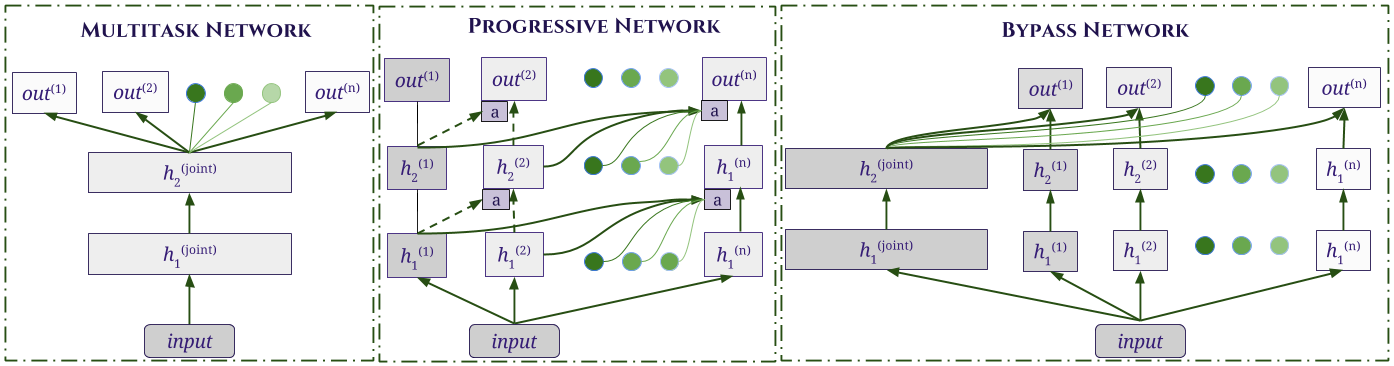
\includegraphics[width=\textwidth]{Images/robust_architectures.png}
  \caption{Left panel depicts a standard multitask architecture. Center panel depicts a progressive architecture. Dotted lines indicate frozen weights. Right depicts our proposed bypass architecture. Note that terms such as ``input'' and ``h'' above denote rows of neurons and not single neurons.}
  \label{fig:arch}
\end{figure}
\subsubsection{Random Forests}
Random forests \cite{breiman2001random} are an ensemble prediction method, where individual decision trees are trained on subsampled subsets of the original dataset. The results for individual trees are averaged to provide the output for the entire system. Random forests are currently widely used in the pharmaceutical industry for QSAR tasks \cite{svetnik2003random}.

We train RF models with 100 trees each, and with
$m/3$ descriptors used at each node, where $m$ is the
number of features in the AP,DP descriptors (using hyperparameters from previous work \cite{ma2015deep}). Tree nodes with 5 or fewer molecules are not split further.  We use the random-forest implementation from Scikit-Learn \cite{pedregosa2011scikit}, but through the DeepChem API for convenience.

\subsubsection{Singletask Architecture}

Singletask deep networks train a separate multilayer neural network for each learning task in the dataset collection. The model for each task is trained separately using backpropagation on the dataset for that task.

\subsubsection{Multitask Architecture}
Multitask deep networks train a joint representation of input datapoints shared for all learning tasks. This shared joint representation is fed into a separate linear model for each dataset in a dataset collection. The entire model is trained end-to-end on training data using backpropagation. The left panel in Figure~\ref{fig:arch} provides a graphical representation of the architecture. Detailed mathematical descriptions have been provided in previous works \cite{ma2015deep, ramsundar2015massively}.

\subsubsection{Progressive Architecture}
The problem of training models capable of solving many tasks is shared by many applications in machine-learning. The progressive neural network architecture \cite{rusu2016progressive} proposes a general solution to this problem by allotting each learning task an independent column of weights. However, the column for task $i$ can refer to all the weights for tasks $1,\dotsc, i-1$ through nonlinear ``adapter'' connections. Progressive networks are trained one task at a time. When task $i$ is training, only the weights in column $i$ are updated. The weights from previous tasks are frozen and may be referred to by the current column but not updated. See the middle panel Figure~\ref{fig:arch} for a graphical depiction of progressive networks, with full detail in the original paper \cite{rusu2016progressive}.

The major drawback of progressive architectures is that the total number of learnable parameters for task $i$ scales linearly with $i$, due to connections to previously learned weights for tasks $1,\dotsc,i-1$. Consequently, for a dataset with $N$ tasks, the total memory requirement scales as $O(N^2)$. For pharmaceutical dataset collections with potentially hundreds of assays, this memory requirement quickly becomes burdensome. Furthermore, the progressive architecture imposes an ordering upon the available tasks. This ordering is often not meaningful for biochemical datasets. For example, a kinase dataset collection may not have a natural notion of which kinase comes first and which comes second in the ordering.

Despite these issues, progressive networks have demonstrated strong results on challenging reinforcement learning and robotics tasks, so we decided to implement and evaluate the effectiveness of progressive architectures for drug-discovery datasets.

\subsubsection{Bypass Architecture}

Progressive architectures allow for each task to have independent nonlinear transformations. The multitask architecture lacks this property, which may render multitask architectures weak on dataset collections with very different tasks. At the same time, progressive architectures lack the shared learnable representations which render multitask architectures powerful. Consequently, we experiment with a bypass architecture that merges the per-task indepedent nonlinearities of progressive networks and the shared learnable layers of multitask networks. The bypass architecture has shared joint layers like the multitask architectures, but also has an independent column of weights which "bypass" the shared representation for each task. However, unlike the progressive architecture, the independent weights for a given task may not interact with the weights for other tasks. This decision prevents the memory growth of progressive networks and also removes the artificial ordering implicit in progressive architectures. See rightmost panel in Figure~\ref{fig:arch} for a depiction of bypass architectures.

\subsubsection{Model Evaluation Metrics}

Model performance is evaluated by using the squared Pearson correlation coefficient ($R^2$) \cite{ma2015deep}. For multitask models, we consider the mean Pearson $R^2$ over all tasks present in the dataset. Since the mean performance only gives a rough sense of relative performance of models, we consider other metrics which measure performance against a random-forest baseline. First, we compute the fraction of learning tasks where performance is improved relative to the random-forest baseline. Past work has noted that multitask models don't offer consistent improvements (many tasks improve performance, but some do worse as well) \cite{ramsundar2015massively}. Computing the fraction improved allows us to understand the failure modes of deep architectures relative to baseline methods. We also compute the largest per-task $R^2$ increase and decrease of deep models compared to random-forest baselines.

These metrics are meant to measure the ``robustness'' of deep-learning architectures. Namely, a robust deep-learning architecture should always outperform baseline methods. While this ideal is not achievable with current architectures, our goal is to evaluate current deep architectures for their degrees of robustness. We propose that robustness is a general principle for proposed architectures, and should be considered in future algorithmic work as a guiding principle.

We also consider inter-task correlations within the raw datasets. Previous work has indicated that multitask learning leverages correlations between tasks in a dataset collection. To provide a rough measure of inter-task correlation, we plot histograms of all pairwise Pearson $R^2$ scores between tasks in a dataset collection. Histograms with large peaks at $0$ indicate that many tasks are uncorrelated with one another; histograms with large peaks at positive values indicate stronger inter task correlations. Note that this visualization is only meaningful for dense datasets; every datapoint has to have a label for every task.

\subsection{Experimental Results}

In this section, we report performance of random forests, multitask networks, progressive networks, and bypass networks trained on the Kaggle, Factors, Kinase and UV dataset collections. Model hyperparameters were tuned on validation sets with a combination of manual hyperparameter tuning and random hyperparameter search \cite{bergstra2012random}. 

\subsubsection{Kaggle}

\begin{table}[h]
    \centering
    \begin{tabular}{ |c|c|c|c| } 
    \hline
    & Mean training $R^2$ & Mean validation $R^2$ & Mean test $R^2$ \\
    \hline
    \textbf{Multitask} & $0.793 \pm 0.005$ & $0.467 \pm 0.014$ & $0.468 \pm 0.012$  \\
    \hline
    \textbf{Progressive} & $0.887 \pm 0.015$ & $0.436 \pm 0.022$ & $0.432 \pm 0.016$  \\
    \hline
    \textbf{Bypass} & $0.843 \pm 0.004$ & $0.454 \pm 0.012$ & $0.456 \pm 0.012$  \\
    \hline
    \textbf{Singletask} & $0.942 \pm 0.002$ & $0.450 \pm 0.009$ &  $0.448 \pm 0.009$ \\
    \hline
    \textbf{Random Forest} & $0.941\pm 0.000$ & $0.423 \pm 0.008$ & $0.428\pm 0.007$  \\
    \hline
    \end{tabular}
    \caption{Model performance on Kaggle Collection. All experiments repeated 3 times with different choice of random seed. Standard deviations are means across per-task standard deviations over trials.}
    \label{tab:kaggle}
\end{table}

\begin{figure}[H]
  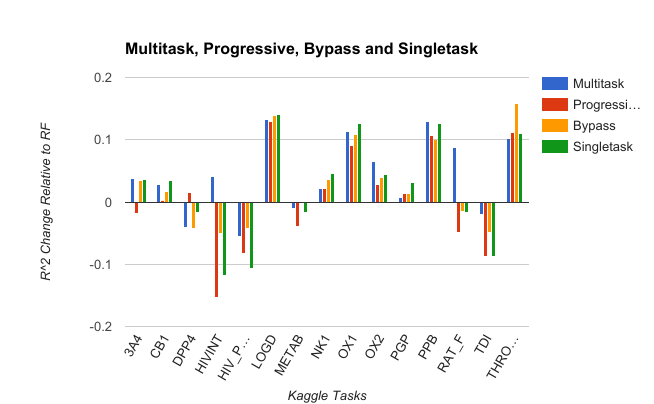
\includegraphics[width=.9\textwidth]{Images/Kaggle_imp.png}
  \caption{Change in performance relative to random forests on Kaggle collection.}
  \label{fig:kaggle-imp}
\end{figure}
\begin{table}[h]
    \centering
    \begin{tabular}{ |c|c|c|c| } 
    \hline
     & Fraction Improved (vs RF) & Largest task $R^2$ drop & Largest task $R^2$ gain \\ 
    \hline
    \textbf{Multitask} & 11/15 & -0.055 & 0.133  \\
    \hline
    \textbf{Progressive} & 9/15 & -0.153 & 0.130  \\
    \hline
    \textbf{Bypass} & 9/15 & -0.050 & 0.157  \\
    \hline
    \textbf{Singletask} & 9/15 & -0.117 & 0.141  \\
    \hline
    \end{tabular}
    \caption{Performance relative to RF baseline on Kaggle test sets.}
    \label{tab:kaggle-comp}
\end{table}

The Kaggle collection serves as a proof of concept that our contributed multitask DeepChem implementation is capable of recapitulating results from the literature \cite{ma2015deep}. Table~\ref{tab:kaggle} reports mean train, validation, and test $R^2$ values for all models on the Kaggle collection. Notably, the singletask and multitask deep architectures achieve performance quantitatively similar to previously reported work, differing only by a couple percentage points (but within previously reported performance ranges for deep networks on this collection). The multitask deep networks offer the strongest validation and test performance of all models tested on the Kaggle collection.

All models overfit the training sets, with mean train $R^2$ significantly higher than mean validation and test $R^2$. Surprisingly, the multitask networks overfit the least, suggesting that the multitask effect acts partially as a regularizer controlling the degree of overfitting. By comparison, both singletask deep networks and random forests have considerably higher training $R^2$ suggesting a greater degree of overfit compared to multitask models. The progressive networks offer comparable performance to random forests, but seem not to perform as well as other deep architectures. The bypass networks behave more similarly to multitask architectures, with strong validation and test performance, but with greater overfitting on the training set, suggesting that the independent bypass layers may harm as well as help.

Table~\ref{tab:kaggle-comp} evaluates the robustness of all deep learning models compared to random forest baselines. Multitask networks perfomed quite robustly with 11 of 15 tasks improved, and worst-case $R^2$ drop of $-.055 R^2$. The bypass networks, singletask, and progressive networks all succeeded in improving 9 of 15 tasks. The progressive and singletask networks suffer more severe per-task $R^2$ drops. Figure~\ref{fig:kaggle-imp} plots the per-task improvement for each model on the Kaggle collection. 

\subsubsection{Factors}
\begin{table}[H]
    \centering
    \begin{tabular}{ |c|c|c|c| } 
    \hline
     & Mean training $R^2$ & Mean validation $R^2$ & Mean test $R^2$ \\
    \hline
    \textbf{Multitask} & $0.941 \pm 0.003$ & $0.517 \pm 0.014$ & $0.424 \pm 0.006$ \\
    \hline
    \textbf{Progressive} & $0.935 \pm 0.001$ & $0.499 \pm 0.001$ & $0.409 \pm 0.005$  \\
    \hline
    \textbf{Bypass} & $0.949 \pm 0.001$ & $0.508 \pm 0.004$ & $0.410 \pm 0.001$ \\
    \hline
    \textbf{Singletask} & $0.954 \pm 0.000$ & $0.504 \pm 0.005$ & $0.393 \pm 0.003$  \\
    \hline
    \textbf{Random Forest} & $0.949 \pm 0.000$ & $0.466 \pm 0.005$ & $0.412 \pm 0.006$ \\
    \hline
    \end{tabular}
    \caption{Model performances on Factors Collection. All experiments repeated 3 times with different choice of random seed. Standard deviations are means across per-task standard deviations over trials.}
    \label{tab:factors}
\end{table}

\begin{figure}[H]
  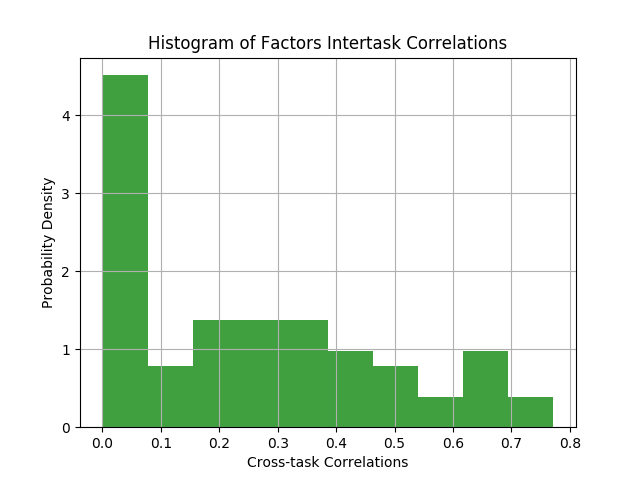
\includegraphics[width=.75\textwidth]{Images/Factors_correlations.png}
  \caption{Histogram of correlations between Factors tasks. The Pearson $R^2$ is computed for each pair of tasks in collection. The histogram displays all computed correlations.}
  \label{fig:factors-corrs}
\end{figure}

\begin{figure}[H]
  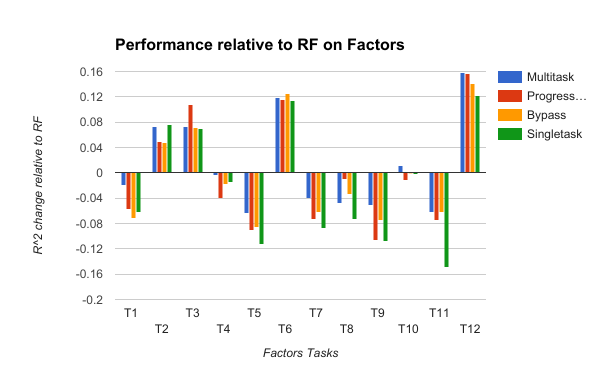
\includegraphics[width=.9\textwidth]{Images/Factors_imp.png}
  \caption{Change in performance relative to random forests on Factors collection. }
  \label{fig:factors-imp}
\end{figure}


\begin{table}[h]
    \centering
    \begin{tabular}{ |c|c|c|c| } 
    \hline
     & Fraction Improved (vs RF) & Largest task $R^2$ drop & Largest task $R^2$ gain \\ 
    \hline
    \textbf{Multitask} & 5/12 & -0.064 & .158  \\
    \hline
    \textbf{Progressive} & 4/12 & -0.108 & .157  \\
    \hline
    \textbf{Bypass} & 4/12 & -.087 & .141 \\
    \hline
    \textbf{Singletask} & 4/12 & -.150 &  .122 \\
    \hline
    \end{tabular}
    \caption{Performance relative to RF baseline on Factors test sets. All experiments repeated 3 times with different choice of random seed. Standard deviations are means across per-task standard deviations over trials.}
    \label{tab:factors-comp}
\end{table}

The Factors collection measures IC50 of inhibition for 12 serine proteases. The measurements for the Factors collection are dense; each molecule is measured in every assay. Figure~\ref{fig:factors-corrs} reports the histogram of correlations between various Factors tasks. While many Factors tasks are effectively uncorrelated, a large proportion of tasks have moderate to high inter-task correlations.

Results for trained models on this collection are reported in Table~\ref{tab:factors} and visualized in Figure~\ref{fig:factors-imp}. The multitask networks achieve the best mean validation and test $R^2$, with the bypass models following closely behind. The Factors collection has only 1500 compounds, compared to the 100 thousand in the Kaggle collection, so perhaps unsurprisingly all models overfit much more heavily than for the Kaggle collection. The multitask effect does not seem to regularize performance on this collection as effectively.

Table~\ref{tab:factors-comp} provides measurements of robustness for the deep models relative to the random forest baseline, and Figure~\ref{fig:factors-imp} provides a graphical representation of model improvement. Perhaps due to the large number of tasks with low correlations, the multitask networks succeed in improving only 5 of 12 tasks. However, tasks that are improved have large boosts in accuracy, while the worst-case drop of $-.064 R^2$ is relatively small. The Progressive, singletask, and bypass models each improve $4$ of $12$ assays, but have worst-case drops larger than for the multitask models.

\subsubsection{Kinase}
\begin{table}[H]
    \centering
    \begin{tabular}{ |c|c|c|c| } 
    \hline
     & Mean training $R^2$ & Mean validation $R^2$ & Mean test $R^2$ \\ 
     %comment MT: R^2
    \hline
    \textbf{Multitask} & $0.897 \pm 0.002$ & $0.301 \pm 0.012$ & $0.238 \pm 0.010$  \\
    \hline
    \textbf{Progressive} & $0.833 \pm 0.012$ & $0.284 \pm 0.006$ & $0.207 \pm 0.001$  \\
    \hline
    \textbf{Bypass} & $0.941 \pm 0.003$ & $0.285 \pm 0.009$ & $0.224 \pm 0.008$  \\
    \hline
    \textbf{Singletask} & $0.951 \pm 0.004$ & $0.284 \pm 0.011$ & $0.229 \pm 0.010$  \\
    \hline
    \textbf{Random Forest} & $0.941 \pm 0.001$ & $0.263 \pm 0.011$ & $0.208 \pm 0.001$  \\
    \hline
    \end{tabular}
    \caption{Model performance on Kinase Collection. All experiments repeated 3 times with different choice of random seed. Standard deviations are means across per-task standard deviations over trials.}
    \label{tab:kinase}
\end{table}
\begin{figure}[H]
  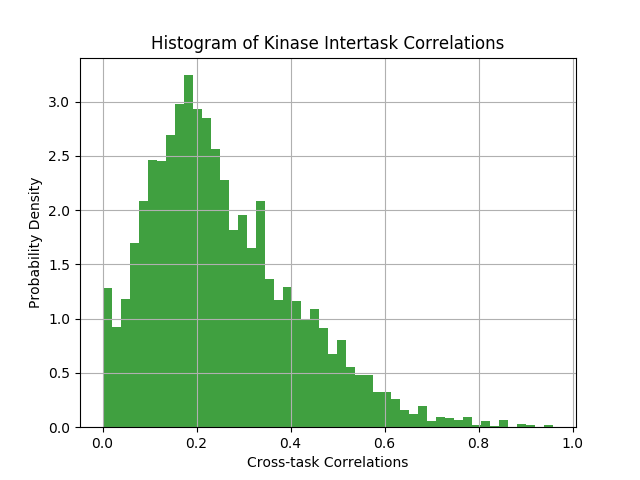
\includegraphics[width=.75\textwidth]{Images/Kinase_correlations.png}
  \caption{Histogram of correlations between Kinase tasks. The Pearson $R^2$ is computed for each pair of tasks in collection. The histogram displays all computed correlations.}
  \label{fig:kinase-corrs}
\end{figure}
\begin{figure}[H]
  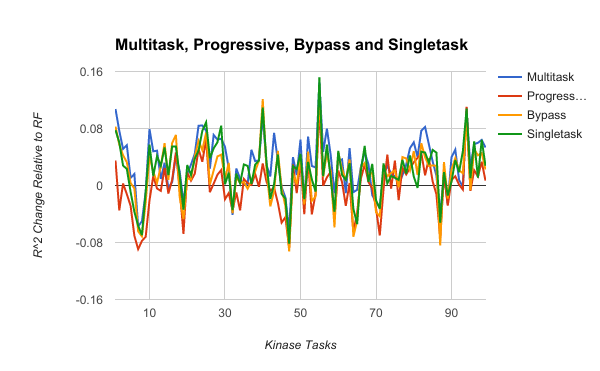
\includegraphics[width=.9\textwidth]{Images/Kinase_imp.png}
  \caption{Change in performance relative to random forests on Kinase collection. Separate lines for each model type are used instead of bars due to large number of tasks.}
  \label{fig:kinase-imp}
\end{figure}

\begin{table}[h]
    \centering
    \begin{tabular}{ |c|c|c|c| } 
    \hline
     & Fraction Improved (vs RF) & Largest task $R^2$ drop & Largest task $R^2$ gain \\ 
    \hline
    \textbf{Multitask} & 79/99 & -0.064 & 0.144  \\
    \hline
    \textbf{Progressive} & 53/99 & -0.089 & 0.111  \\
    \hline
    \textbf{Bypass} & 74/99 & -0.093 & 0.131  \\
    \hline
    \textbf{Singletask} & 78/99 & -0.082 & 0.152  \\
    \hline
    \end{tabular}
    \caption{Performance relative to RF baseline on Kinase test sets.}
    \label{tab:kinase-comp}
\end{table}

The Kinase collection consists of 2500 compounds tested against 99 kinase assays. This collection like Factors (and unlike Kaggle) is dense, with all molecules measured in all assays.  Figure~\ref{fig:kinase-corrs} reports the histogram of correlations between various Kinase tasks, displaying that most tasks have moderate to strong correlations with other tasks in collection.

Table~\ref{tab:kinase} reports mean train, validation, and test $R^2$ of trained models on this collection and Figure~\ref{fig:kinase-imp} displays graphically performance relative to random forest baseline. Multitask models demonstrate the strongest performance on both validation and test sets. Progressive networks again achieve performance similar to random-forests, with the bypass and singletask models offering performance between random forests and multitask architectures. Given the greater number of compounds, the multitask networks once again overfit less severely than singletask deep networks and random forests. Notably, progressive networks appear to underfit this dataset, and achieve the lowest training $R^2$. This underfit is likely due to memory issues; to handle training of progressive networks with 99 tasks (recall that memory usage scales as $O(N^2)$ where $N$ is the number of tasks), we limited the number of hidden nodes per task (per layer) to $50$, which may have reduced the models' explanatory capacity.

Table~\ref{tab:kinase-comp} evaluates the robustness of the deep learning methods relative to the random forest baseline. The multitask networks are quite robust on this collection, providing improvements for 79/99 assays. This broad improvement may be due to the fact that kinase inhibitors are often promiscuous across many kinases \cite{anastassiadis2011comprehensive}, suggesting that shared representations can be easily extracted. (Figure~\ref{fig:kinase-corrs} supports this assertion.) The worst case performance drop of $-.064 R^2$ for multitask models is moderate, suggesting that multitask methods are strong models for Kinase systems. The bypass and singletask models also succeed in offering broad improvement, respectively for 74/99 and 78/99 assays, but with slightly larger worst-case drops of $-.089 R^2$ and $-.082 R^2$ respectively. The progressive models only improve 53/99 assays relative to random forests, possibly due to the model's inability to exploit intertask correlations.

\subsubsection{UV}
\begin{table}[h]
    \centering
    \begin{tabular}{ |c|c|c|c| } 
    \hline
     & Mean training $R^2$ & Mean validation $R^2$ & Mean test $R^2$ \\
    \hline
    \textbf{Multitask} & $0.961 \pm 0.001$ & $0.420 \pm 0.013$ & $0.441 \pm 0.014$  \\
    \hline
    \textbf{Bypass} & $0.903 \pm 0.005$ & $0.396 \pm 0.014$ & $0.421 \pm 0.014$  \\
    \hline
    \textbf{Singletask} & $0.968 \pm 0.002$ & $0.399 \pm 0.012$ & $0.417 \pm 0.013$ \\
    \hline
    \textbf{Random Forest} & $0.961 \pm 0.000$ & $0.404 \pm 0.006$ & $0.428 \pm 0.006$  \\
    \hline
    \end{tabular}
    \caption{Model performance on UV Collection. All experiments repeated 3 times with different choice of random seed. Standard deviations are means across per-task standard deviations over trials. Progressive networks were omitted since models took over a day to train.}
    \label{tab:uv}
\end{table}

\begin{figure}[H]
  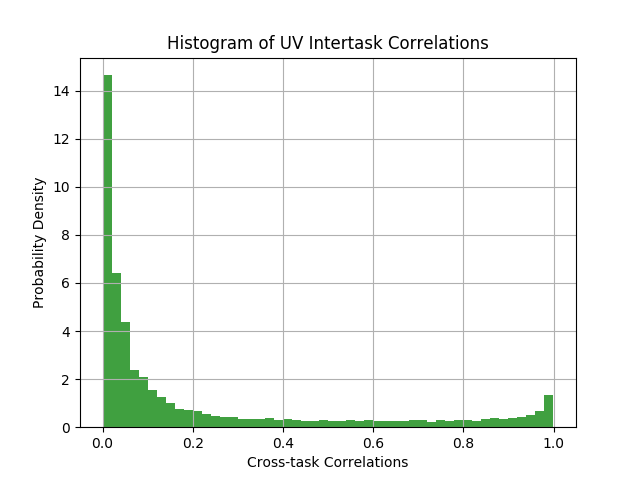
\includegraphics[width=.75\textwidth]{Images/UV_correlations.png}
  \caption{Histogram of correlations between UV tasks. Pearson $R^2$ is computed for each pair of tasks in collection. Histogram displays all computed correlations.}
  \label{fig:uv-corrs}
\end{figure}
\begin{figure}[H]
  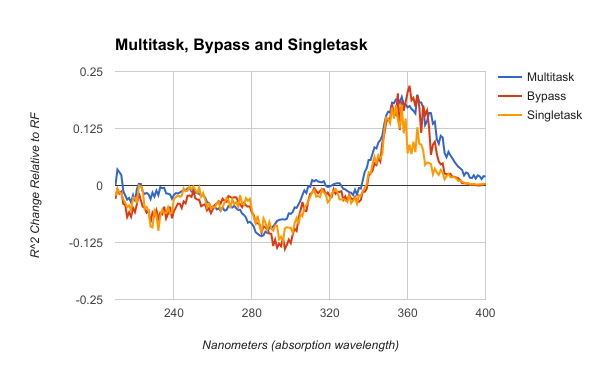
\includegraphics[width=.9\textwidth]{Images/UV_imp.png}
  \caption{Change in performance relative to random forests on UV collection. Separate lines for each model type are used instead of bars due to large number of tasks.}
  \label{fig:uv-imp}
\end{figure}
\begin{table}[h]
    \centering
    \begin{tabular}{ |c|c|c|c| } 
    \hline
     & Fraction improved (vs RF)  & Largest task $R^2$ Drop & Largest task $R^2$ gain \\ 
    \hline
    \textbf{Multitask} & 81/190 &  -.111 & 0.199  \\
    \hline
    \textbf{Bypass} & 60/190 & -0.139 & 0.219  \\
    \hline
    \textbf{Singletask} & 63/190  & -0.122  & 0.177  \\
    \hline
    \end{tabular}
    \caption{Performance relative to RF baseline on UV test sets.}
    \label{tab:uv-comp}
\end{table}


The UV dataset collection consists of roughly 10,000 compounds evaluated over 190 absorption wavelengths (210-400 nm). The UV collection (like the Factors and Kinase collections) is dense, with all molecules measured at all wavelengths. Figure~\ref{fig:uv-corrs} reports the histogram of correlations between various UV tasks. Unlike other collections, most assays are weakly correlated. The small bump at high correlation is due to fact that absorption at nearby wavelengths is highly correlated (absorption at 231nm and 232nm likely have high correlation for example).


Table~\ref{tab:uv} reports mean train, valid, and test $R^2$ values for models on this dataset collection. Multitask models achieve the highest mean validation and test $R^2$, but only by a slight margin. Note that Table~\ref{tab:uv} does not provide numbers for progressive networks. We could not successfully train progressive models on this collection within a day, likely due to the high graph complexity for a progressive architecture with nearly 200 tasks.

Table~\ref{tab:uv-comp} evaluates robustness of trained models relative to the random forest baseline. Notably, multitask models don't succeed in outperforming the random forest baseline on a majority of assays, with only 81 of the
190 datasets improved. As with Factors, the large number of uncorrelated tasks may have contributed to this outcome. The largest worst-case $R^2$ drop is moderate, with $-.111 R^2$ drop observed on one task, but with large performance gains of $0.199$ on the best-improved task. Figure~\ref{fig:uv-imp} shows an interesting pattern, with most assays underperforming the RF baseline, but with a large fraction showing significant improvements over the RF baseline. The improved assays are all adjacent, indicating that the multitask models may perhaps be learning some shared property of the physics at these wavelengths.


\subsubsection{Singletask versus Multitask}
\begin{table}[h]
    \centering
    \begin{tabular}{ |c|c|c| } 
    \hline
     Dataset Collection & Multitask Improved \\ 
    \hline
    \textbf{Kaggle} & 8/15  \\
    \hline
    \textbf{Factors} & 11/12  \\
    \hline
    \textbf{Kinase} & 64/99  \\
    \hline
    \textbf{UV} & 155/190 \\
    \hline
    \end{tabular}
    \caption{Number of tasks improved by multitasking.}
    \label{tab:tasks-improved}
\end{table}

To evaluate the relative improvement due to the multitask effect, as opposed to changes in performance due to deep learning, we evaluated the fraction of tasks where multitask models outperformed singletask models for all collections we consider. Results are displayed in Table~\ref{tab:tasks-improved}. Notably, a majority of assays in all collections show improvement of multitask over singletask, indicating that multitask deep-learning performs better on our assay collections than singletask deep learning.

\subsection{Discussion and Conclusion}

Preliminary studies have demonstrated that multitask deep learning can offer performance improvements over simpler machine-learning techniques for drug-discovery datasets \cite{ma2015deep, ramsundar2015massively}. However, multitask deep networks have yet to achieve a wide degree of adoption across the pharmaceutical and biotechnology industries. Historically, transforming machine learning prototypes into production systems can be challenging. As noted previously, Netflix decided not to use the winning entry in its million dollar recommendation challenge to serve actual customer recommendations \cite{netflixNever}. We hypothesize that two key barriers prevent the widespread adoption of multitask deep networks: First, implementing deep architectures can be a challenging software endeavor. Second, the failure modes of multitask deep networks relative to random forest and singletask baselines remain poorly understood.

This work has aimed to overcome both barriers to entry for deep architectures. To overcome software challenges, we have introduced a high-quality open-source implementation of multitask deep-networks as part of the DeepChem library for open-source drug-discovery \cite{deepchem}. Our implementation makes it easy to build, fit, and evaluate high quality deep-learning models with simple python scripts (see Figure~\ref{fig:code} for a real code example). We also contribute open-source implementations of two new deep-learning architectures to DeepChem. Progressive networks \cite{rusu2016progressive} were first proposed for robust multitask deep learning in robotic and reinforcement learning applications. We also propose a bypass architecture, which aims to serve as a hybrid of multitask and progressive architectures. 

We used our open source DeepChem implementation to test the behavior of our deep architectures across four broad collections of datasets. We demonstrated that the DeepChem implementation can duplicate qualitatively and quantitatively the performance of deep models on the Kaggle collection analyzed previously in the literature \cite{ma2015deep}. We then evaluated the performance of multitask, singletask, progressive, bypass, and random forests across the Factors, Kinase, and UV dataset collections. In particular, since our validation and test splits use time and neighbor-split (known to be challenging for multitask methods), our evaluation constitutes a ``worst-case'' test of multitask performance. Even under these challenging conditions, multitask models offer the strongest mean validation and test set $R^2$ across all evaluated collections. 

To further evaluate model performance, we introduced a set of robustness measurements, which measure the fraction of assays improved by deep architectures relative to random forest baselines. We also considered the worst-case and best-case per-task $R^2$ improvement over all tasks. Multitask architectures are more robust than progressive, singletask, and bypass architectures on these datasets, with a majority of assays improved over RF on the Kaggle and Kinase dataset. On the Factors and UV datasets, fewer assays are improved, likely due to lower inter-task correlations, but some tasks see quite significant improvements and only moderate performance drops elsewhere. Worst-case performance drops are lowest for multitask architectures compared to other deep architectures. Broadly, our robustness analysis suggest that multitask deep-models can offer improvements over random forests for a wide variety of models, and especially in collections with high inter-task correlations. Our work suggests that multitask architectures can be fruitfully applied to many datasets that arise in drug discovery.  

%%% NEW PARAGRAPH

In general, we note that while multitask deep learning provides improvements over random forest methods on average, many assays suffer worse performance compared with the random forest baseline. While the full investigation of these failures is left to future work, we note that the use of obfuscated fingerprints that obscure molecular structures may be limiting the potential of deep learning methods on these datasets. Subsequent work by some of the authors of the present paper has shown that graph convolutional models \cite{duvenaud2015convolutional} implemented in DeepChem can achieve significant boosts in performance over multitask deep networks on the MoleculeNet benchmark suite \cite{wu2017moleculenet}. In the future, it may be interesting to test these graph convolutional methods in collaboration projects on pharmaceutical data. The DeepChem library will hopefully serve to enable such research.

%%% NEW PARAGRAPH

%%% NEW PARAGRAPH

We note that in this paper, we did not attempt to place error bars on the predictions made for individual molecules. The presence of good error bars allows practitioners to reason about the domain of applicability for learned models. However, gauging the confidence of predictions from deep learning models is known to be challenging. There has been significant recent interest in the methods of Bayesian deep learning \cite{kendall2017uncertainties}, which may provide a structured solution to the uncertainty modeling problem. Extending Bayesian deep learning methods to pharmaceutical applications is beyond the scope of the present work however, and we suggest it as a good topic for future work.

%%% NEW PARAGRAPH

Our open-source multitask deep network implementation in DeepChem can help facilitate the broad adoption of deep networks in commercial drug discovery. In particular, we open source our deep learning models for all collections in this paper (along with the associated datasets) to serve as a community resource. We anticipate that our open-source implementation in tandem with our statistical robustness analysis across a broad collection of datasets will facilitate the widespread adoption of multitask deep-learning in the pharmaceutical industry.


\subsection{Acknowledgements}

We would like to thank the Stanford Computing Resources for providing us with access to the Sherlock and Xstream GPU nodes. Thanks to Junshui Ma for help in debugging performance on the Kaggle collection. Thanks to Kevin McCloskey and Patrick Riley from Google for open-sourcing the code that formed the preliminary DeepChem multitask implementation. Thanks to Aarthi Ramsundar for help with diagram construction.

The Pande Group is broadly supported by grants from the NIH (R01 GM062868 and U19 AI109662) as well as gift funds and contributions from Folding@home donors.

We acknowledge the generous support of Dr. Anders G. Fr{\o}seth for our work on machine learning.

B.R. was supported by the Fannie and John Hertz Foundation.

AV, MT, RPS are employees of Merck \& Co., Inc. of Kenilworth, NJ. VSP is a consultant and SAB member of Schrodinger, LLC and Globavir, sits on the Board of Directors of Apeel Inc, Freenome Inc, Omada Health, Patient Ping, Rigetti Computing, and is a General Partner at Andreessen Horowitz.


%\clearpage
%\section{Computational Modeling of $\beta$-secretase 1 (BACE-1) Inhibitors using Ligand Based Approaches}

This chapter is adapted from: 

Govindan Subramanian, Bharath Ramsundar, Vijay Pande, and Rajiah Aldrin Denny. "Computational modeling of β-secretase 1 (BACE-1) inhibitors using ligand based approaches." Journal of chemical information and modeling. \cite{subramanian2016computational}.

I was the second author and worked on conception of the original idea, implementation and execution of machine learning experiments, and writing of the paper.

\subsection{Abstract}
The binding affinities (IC50) reported for diverse structural and chemical classes of human $\beta$-secretase 1 (BACE-1) inhibitors in literature were modeled using multiple in silico ligand based modeling approaches and statistical techniques.  The descriptor space encompasses simple binary molecular fingerprint, 1- and 2-dimensional constitutional, physicochemical and topological descriptors, and sophisticated 3-dimensional molecular fields that require appropriate structural alignments of varied chemical scaffolds in one universal chemical space.  The affinities were modeled using qualitative classification or quantitative regression schemes involving linear, non-linear, and deep neural network (DNN) machine-learning methods used in the scientific literature for quantitative structure activity relationships (QSAR).  In a departure from tradition, ~20\% of the chemically diverse dataset (205 compounds) was used to train the model with the remaining ~80\% of the structural and chemical analogs used as part of an external validation (1273 compounds) and prospective test (69 compounds) sets respectively to ascertain the model performance.  The machine learning methods investigated herein performed well in both the qualitative classification (~70\% accuracy) and quantitative IC50 predictions (RMSE ~ 1 log).  The success of the 2D descriptor based machine learning approach when compared against the 3D field based technique pursued for hBACE-1 inhibitors provides a strong impetus for systematically applying such methods during the lead identification and optimization efforts for other protein families as well.


\subsection{Introduction}

In silico computer assisted drug design (CADD) plays an integral part in several areas of preclinical small molecule drug discovery \cite{sliwoski2014computational}.  Ligand- and structure-based modeling approaches enable small molecule scientific discovery research teams to prioritize the compound progression pathways from the initial hit identification to the final clinical candidate nomination in the organization’s research and development portfolio \cite{ekins2007silicoA, ekins2007silicoB, macalino2015role}.  One of the key parameters in the optimization path to the development candidate involves the small molecule affinity improvement to its intended therapeutic target.  

When the structure of the small molecule bound to its protein is available, high bias is often used to apply structure-based design (SBD) techniques \cite{anderson2003process} to guide further affinity improvement efforts, since the x-ray structure of the complex provides a great deal of insight into the key drivers modulating affinity.  In fact, SBD approaches like docking work under the premise of the identified or hypothesized binding site \cite{kuntz1982geometric,kitchen2004docking}.  The shape and curvature of the binding pocket as well as the computed molecular grids representing them determine the plausible orientation and fit of the synthetic compound under consideration, resulting in qualitative rank ordering of in silico screened small molecule ligands binding to the target.  Thereafter, high end molecular dynamics simulation is used to assess the binding affinity quantitatively and more accurately ($\Delta \text{Gbind}$) \cite{homeyer2014binding, wang2015accurate, aldeghi2016accurate, de2016role} with implicit solvation methods currently offering a trade-off for computational cost and accuracy in predicting binding affinity.  Among the shortcomings of the SBD approach, the plasticity of the protein active site residues upon ligand binding (induced fit) creates uncertainties that could not be handled straightforwardly by the use of a single protein-ligand complex structure \cite{craig2010ensemble, korb2012potential}.  This necessitates the use of multiple protein structures (ensemble docking) to understand and predict ligand affinities, a process that often adds noise and computational cost when compared to the potential benefit \cite{grebner2016binding}.  Even though there has been a steady increase in the use of SBD approaches for quantitative affinity prediction,, the approaches are still considered to be in their infancy and are often unable to provide consistent accuracy across a range of targets to be applied routinely \cite{wang2015accurate}.

On the other hand, ligand-based design (LBD) methods with QSAR \cite{hansch1962correlation, cherkasov2014qsar}, statistical fits dominated the field during the last six decades due to the scarcity of solved ligand bound protein x-ray structures.  These methods use common features in the chosen ligand set without any apriori knowledge of the environment surrounding the small molecule.  Traditional LBD approaches like the pharmacophore \cite{sanders2012comparative, wolber2015pharmacophore}, and molecular field \cite{cramer1988comparative} based model employing molecular alignments uses known experimental activity information from a preselected compound set to guess the potential microenvironment around the ligand and applies a statistical fit to predict the activity of the unknowns or new design modifications.  The sheer publication and citation volumes using these techniques stand as a testament to the success and acceptance of such pseudoreceptor approaches by the CADD community.  

Although the strengths and limitations of the two major computational approaches described above and routinely used in in silico drug discovery could be debated, the complementarity of the SBD and LBD approaches can enable the field to progress further by using their hybrid \cite{drwal2013combination, broccatelli2014best, huang2015hybriddock, prathipati2015integration}.  For instance, the binding mode of ligands to their intended target can be identified using SBD methods or x-ray structures of ligand bound protein complex and a quantitative evaluation of the affinities computed using established 3D QSAR approaches \cite{klebe1999comparative, cappel2015exploring}, by overlaying related structural analogs (using maximum common substructure) to the bound orientations of the ligand in the x-ray structure or via docking protocols.  We and other groups have started to realize enhanced benefits using such combinations with high success rates in prediction \cite{subramanian2012integrated, urniaż2013x,therese2014multiple,cramer2014templateA,cramer2014templateB}.  Herein, we demonstrate that such an approach can now be applied to systems with a very limited data set size and diverse chemical scaffolds.   To compare the effectiveness of such hybrid approaches, multiple LBD techniques, starting from simple Bayesian methods to sophisticated machine-learning methods, were applied for the same dataset to assess the computational ease vs. prediction accuracy as the feature complexity (1D to 3D) and information content (fingerprints to molecular fields) were incremented gradually.

The target selected for this computational exercise is BACE-1, a long sought potential therapeutic target for Alzheimer’s \cite{haass2007soluble,walsh2007abeta}.  This aspartyl protease is considered to be the key driver for the brain amyloid β accumulation and has eluded pharmaceutical and biotechnology companies alike in delivering a small molecule drug for over a decade \cite{cummings2014alzheimer}.  The BACE-1 orthosteric active site utilizes two aspartate residues (D32 and D228) to anchor endogenous substrates or synthetic ligands (Figure \ref{fig:bace_scheme1}) and is located in between the N- and C-terminal domain.  The shallow and highly exposed binding site is shielded by an extremely flexible β hairpin loop (Y68 - A77) that adapts multiple flap conformations \cite{xu2012flexibility} depending on the bound ligand that either disturbs or perturbs the active site water network based on the nature (closed/open) of the flap configuration \cite{shimizu2008crystal, manoharan2015target}.  In addition, the BACE-1 activity shifts depending on the pH as well as the protonation states of the catalytic dyad \cite{domínguez2010effect, ellis2015ph}.  Such complexities have rendered it very difficult to model and interpret the effect of the thermodynamic contributions (enthalpy, entropy, etc.) obtained through biophysical experimental measurements to the small molecule BACE-1 inhibitor binding \cite{geschwindner2015ligand}.  

\begin{figure}
  \centering
  \begin{subfigure}
  \centering
  \includegraphics[width=0.9\textwidth]{Images/bace_scheme1.jpg}
  \end{subfigure}
  \begin{subfigure}
  \centering
  \includegraphics[width=0.9\textwidth]{Images/bace_scheme1B.png}
  \end{subfigure}
  \caption{Scheme 1.  Depiction of BACE-1 binding site (top) using the ligand from PDB code 3UQP along with the protein-ligand interaction (bottom)}
  \label{fig:bace_scheme1}
\end{figure}


Although scientific rigor alongside computational and experimental interplay can enable a much deeper understanding of the key factors influencing binding, they are more often restricted to the specific chemical series that was used for interrogation in the binding affinity optimization cycle.  It is seldom that such learning can be extended widely and hence provides limited value to the broader scientific community.  To circumvent such limitations and expand the scope to address several BACE-1 inhibitor chemical and structural classes, multiple LBD approaches were pursued to identify the sweet spot between computational rigor and trade-off for meaningful compromise that would allow rapid and routine evaluation of new compound ideas in the day-to-day iterative lead optimization cycle.  

\subsection{Methods}

The current dataset includes 1,547 synthetic human BACE-1 inhibitors reported in scientific literature over the past decade with protein…ligand x-ray structures available for over 250 of them in the PDB \cite{rose2010rcsb}.  Experimental IC50’s are also reported for 1,486 compounds and Kd/Ki reported for another 43.  The dataset covers compounds originating from at least 30 different laboratories that include academia, biotechnology, and pharmaceutical companies and spans across the globe in terms of their origin, cautioning on the inhomogeneity of experimental observation \cite{kramer2016comprehensive} used for statistical modeling.  The structures and reported activities for all the compounds were retrieved from either ChEMBL \cite{gaulton2011chembl} or from the original source publication using the citation information from PDB.  In assembling the ligand dataset, only publications that reported a solved x-ray ligand…BACE-1 structure was considered as this provides a reasonable premise to guess on the potential binding mode (bioactive conformation) of the closely related medicinal chemistry derived analogs reported in the same article as part of the structure-activity relationship (SAR).  We have made the ligand dataset publicly available in a convenient CSV format \cite{wu2017moleculenet}.

The physicochemical attributes for the 1547 ligand dataset were computed using BIOVIA’s Pipeline Pilot \cite{systemes2016biovia} and vary between 138 to 1350 for molecular weight (MW); -6.6 to 7.4 for logD; -5.1 to 7.6 for AlogP; 16 to 525 for polar surface area (PSA); 0 to 18 for H-bond acceptor (HBA); 1 to 15 for H-bond donor (HBD); 0 to 40 rotatable bonds; 10 to 90 for heavy atom counts for the reported experimental pIC50’s ranging from 2.5 to 9.5.  As would be apparent, the chemistry captures very small synthetic fragments and large molecular weight oligopeptide and their mimics.  The ligand efficiency (LE) varies between 0.2 to 0.5, binding efficiency index (BEI) ranges from 8 to 22, and the surface efficiency index (SEI) mostly between 4 and 12 \cite{abad2010ligand}.  A distribution of the various physicochemical property profiles (Supporting information S2) reveal that the dataset attributes is not skewed and spans the individual space with a Gaussian spread.  
The global 3D alignment of all the analogs from multiple chemical scaffolds was achieved by following the steps outlined in Figure \ref{fig:bace_scheme2}.  Chain A of 2QP8 (PDB code) was used as the reference, as this structure had one of the best available resolutions (1.5Å) reported when this work was initiated.  Each of the reported PDB structures for the BACE-1…inhibitor x-ray complex was structurally aligned to the above reference using the structalign script available within the Schrödinger’s MAESTRO \cite{maestrorelease20142} suite of programs.  The protein, metal ions, and solvent were subsequently removed from the aligned structures and only one ligand structure from each PDB entry was retained for further processing.  The structure data file built based on protein superposition (containing all the aligned ligands) was uploaded to the molecular database spreadsheet within MOE \cite{moeversion2012chemical} from Chemical Computing Group.  The ligands were subsequently cleaned (bond orders fixed) and prepared by the addition of hydrogens and molecular charges as deemed appropriate.  This procedure now provides an alignment of the diverse ligands in a universal chemical space as would be seen by the protein target.  It also minimizes the pharmacophore and shape bias elicited by the molecular superposition algorithms, and underpins the notion that structurally similar ligands need not bind in a similar way. \cite{subramanian2012integrated}

\begin{figure}
  \centering
  \includegraphics[width=0.9\textwidth]{Images/bace_scheme2.png}
  \caption{Scheme 2. Workflow for the Training, Test, and Validation Set Compound Alignment Used for 3D-Field Based Approaches.}
  \label{fig:bace_scheme2}
\end{figure}

The 274 compounds assembled in this manner (x-ray of aligned hBACE-1…ligand complex) formed the basis of the training (205) and test (69) sets respectively and were used for the 3D molecular alignment dependent approaches pursued in this study.  Since the bioactive conformation for each ligand is now identified (based on the x-ray complex), all medicinal chemistry derived structural analogs within each scaffold reported as part of the SAR exploration in the respective publication were aligned to each individual reference x-ray structures (Figure \ref{fig:bace_scheme2}, right) to yield the final 1,273 validation set analogs that did not have an experimental x-ray structure disclosed in public literature.  No similarity cutoff threshold was used for the SAR compounds since these were standard R-group analogs belonging to the same chemotype that is represented by the x-ray structure reported in the same publication.

The alignment protocol follows the procedure described earlier in literature. \cite{subramanian2012integrated}  Specifically, the ligand coordinates extracted from the BACE-1 complex x-ray structure reported in each individual publication was used as the reference frame (Figure \ref{fig:bace_scheme2}, right) and the SAR analogs reported in that publication were superposed to the chosen reference using the fragment\_superpose and flexalign\_manual svl scripts available from MOE.  Further refinement was achieved through subtle constrained minimization of each of the aligned ligand to achieve maximum overlay with the reference structure per the refine option implemented within the flexalign\_manual.svl script.  This procedure of choosing the individual x-ray reference and SAR analogs was iterated for each publication (see S1 supporting information) and the consolidated alignment of all the reference compounds (now part of the training set) and the SAR analogs (now part of the validation set) comprise the full dataset used for the modeling exercise. 

An additional 69 ligand bound x-ray structures were grouped as the prospective test set since these complexes do not have reported IC50 values, but some of them have either Ki/Kd disclosed instead.  The predicted binding affinities would then offer a decent starting point if scaffold hopping exercise need to be pursued for any of these chemical series.   Succinctly, the published x-ray of BACE-1…ligand complex constituted the source of the 205 training set compounds and the reported SAR in scientific literature formed the basis of the 1273 validation set molecules such that the latter has at least one close representative in the training set. 
In order to ascertain if such strenuous computational rigor described above is required to obtain statistically meaningful and robust predictive QSAR models, additional LBD approaches were also pursued.  These include the standard QSAR approaches that use the traditional binary fingerprints or molecular descriptors as computed by Canvas \cite{canvasrelease20131} from Schrödinger.  For instance, the 1000 most informative bits from linear, radial, dendritic, and MolPrint2D fingerprints \cite{sastry2010large,an2013kernel}, were used to develop qualitative classification models while the constitutional, physicochemical and topological descriptors computed using Canvas were used to build quantitative regression models.  Both the qualitative and quantitative models included linear, non-linear, and deep learning techniques \cite{ramsundar2015massively}.  Such a thorough coverage of the interdependence of dataset, descriptor, and statistical approach for one protein target represented by diverse chemical scaffolds should provide standard baselines when approaching similar problems in a lead identification or optimization cycle within a preclinical drug discovery setting.

\subsection{Results}

\subsubsection{Chemistry Space}
Prior to analyzing the outcomes from the different approaches and models, it is pertinent to chart out the chemical space occupied by the training and validation set BACE-1 inhibitors as this would provide some granularity for the well-recognized model applicability domain concerns \cite{sheridan2015relative}.  Since the model generation involved multiple descriptor features, the chemical space was generated using the same feature space.  The first three principal components (PC) were computed using extended connectivity fingerprint (ECFP6) \cite{rogers2010extended}, Canvas constitutional, physicochemical, and topological descriptors \cite{sastry2010large}, as well as Bemis-Murcko Tier-1 (topography with atomtype annotation) or Tier-2 (topography) molecular framework scheme \cite{bemis1996properties}.  Figure \ref{fig:bace_1} depicts the scatter plot of the PC1 and PC2 space derived from some of the procedures mentioned above.  As would be expected, the Tier-2 reflects the minimal diversity points in the compound space since this represents the 2-dimensional (2D) shape and geographical topology of the varying chemotypes considered in this study.  The 2D skeleton terrain sheds light on the chemical framework heterogeneity (Figure \ref{fig:bace_1A}) within a dimensionality reduction visualization context, with the expected homogenous distribution (overlap) for the validation set around the training set compounds.  An alternate perspective obtained using the radial ECFP6 fingerprints captures the subtle and varied contours and represents a few clusters (Figure \ref{fig:bace_1B}).  A pairwise comparison of the training set compounds using ECFP6 fingerprint and Tanimoto similarity computed via Canvas is provided in supporting information S3.  The macroscopic chemistry space view obtained by computing the various constitutional, physicochemical, and topological properties together reflect on the broad property based diversity of the inhibitors considered.  The scatter distribution, being continuous and not overly islandic, also provides enough motivation to have confidence in the models being developed.  The plots also highlight that the positioning of the validation set in comparison to the training set compounds is not unreasonable to raise concerns in the predictive capability (model applicability domain) of the models being developed using either the fingerprint or descriptor space (Figure \ref{fig:bace_1C}).

\begin{figure}
\centering
\begin{subfigure}
  \centering
  \includegraphics[width=0.3\textwidth]{Images/bace_figA.png}
  \caption{A)  Tier 2 Bemis-Murcko framework}
  \label{fig:bace_1A}
\end{subfigure}
\begin{subfigure}
  \centering
  \includegraphics[width=0.3\textwidth]{Images/bace_figB.png}
  \caption{B) ECFP6 fingerprints}
  \label{fig:bace_1B}
\end{subfigure}
\begin{subfigure}
  \centering
  \includegraphics[width=0.3\textwidth]{Images/bace_figC.png}
  \caption{C) Canvas descriptors}
  \label{fig:bace_1C}
\end{subfigure}
\begin{subfigure}
  \centering
  \includegraphics[width=0.3\textwidth]{Images/bace_fig1D.png}
  \caption{ D) Scaffold grouping on a SOM for the training (blue), validation (green), and test (red) set compounds.}
  \label{fig:bace_1D}
\end{subfigure}
\caption{PCA plot for the 1547 BACE-1 inhibitors.  Training, validation, and test set compounds colored in blue, green and red respectively.}
\label{fig:bace_1}
\end{figure}

Two dimensional self-organizing map (SOM) \cite{kohonen1998self} is another dimensionality reduction technique that provides an orthogonal viewpoint compared to the previous approaches \cite{osolodkin2015progress}. The outcome from SOM using the Canvas descriptors is shown in Fig. 1d.  It should be noted that the SOM implementation in DataWarrior \cite{sander2015datawarrior}, uses Rubberbanding forcefield approach that translates the similarity better than the traditional PCA.  Since the SOM clustering is based on similar compound pairs and neighborhood relations, the diversity of the chemical scaffolds considered in this study is reminiscent in the distinction shown between the topological neighbors and close neighbors.  The SOM depiction in Fig. 1d also shows that majority of the training and validation set compounds have clear topographical neighbors, while the training and test set compounds offer additional close neighbors that can potentially be exploited for SAR exploration, if needed. 

\subsubsection{Biological Property Landscape}

Although the unsupervised approaches for modeling the chemical space present a clean picture of confidence for pursuing modeling activities, additional evaluations were undertaken on the dataset to delineate potential disconnects in the biological property space being modeled when relatively minimal changes are incorporated to the structure.  The SkeletonSphere descriptor scheme implemented in DataWarrior \cite{sander2015datawarrior} was used for the chemical descriptions of the training and validation datasets. The structure activity landscape index (SALI) \cite{guha2008structure} that provides a disconnect measure between the biological observation ($\Delta \text{pIC50}$) and the extent of chemical diversity (1 – similarity) for each compound pair was subsequently computed and incorporated within Figure \ref{fig:bace_2A} of the affinity (pIC50) scatter plot for each of the molecule pair being compared.  Approximately 2,765 pairs were identified using a similarity cut-off threshold of 95\% (Supporting information S4).  Among these, only 51 pairs can be attributed solely to the training set and this provides another inference for the compound diversity within the training dataset.  Among the 2,714 chemical similarity pairs within the validation set, activity cliffs $\geq 2$ log units are exhibited by at least 102 pairs representing ~4\% of the validation set.  These experimental observations suggest instances where subtle changes to structure has profound impact on the IC50 being measured in spite of the conserved modifications to the structure.  While such biological property space ruggedness cautions on the predictive capabilities of the in silico models being developed, it should be emphasized that the overall terrain is pretty smooth with ~2,200 pairs exhibiting $\Delta \text{pIC50} < 1$ log unit.  Irrespective of the model performance on the molecules that demonstrate activity cliffs, the experimental observations shed light on the expected microenvironment (steric, electrostatic, H-bond, etc.) hotspots that need to be paid attention to, besides the black box modeling outcome.  


Figure \ref{fig:bace_2B} provides a visual depiction of the relationship between the observed experimental affinities with respect to the similarities in the chemical space computed using SkelSpheres descriptors implemented in DataWarrior \cite{sander2015datawarrior}.  The key observation is the finding that training set compounds (blue squares) are spread across the validation set compounds, although not being blown out extensively.  The near neighbors in the validation set that surrounds the training set based on similarity and the SALI index (square size) shows that the biological environment is also smooth to a major extent albeit the anticipated cliffs observed in some instances within the clustered compounds.  
Thus, the analysis of the chemical and biological space reveals that the dataset and modeling space [fingerprints/descriptors] should result in productive and predictive models that could guide affinity optimization efforts for hBACE-1 protein target.

\begin{figure}
\centering
\begin{subfigure}
  \centering
  \includegraphics[width=0.9\textwidth]{Images/bace_fig2A.png}
  \caption{a) SALI plot of compound pairs (training and validation) with >95\% similarity.  The x and y axis represent the experimental pIC50 activity values of the compound pairs being plotted (see S4 supporting information).}
  \label{fig:bace_2A}
\end{subfigure}
\begin{subfigure}
  \centering
  \includegraphics[width=0.9\textwidth]{Images/bace_fig2B.png}
  \caption{b) Activity cliffs (marker size) for the training and validation set grouped based on their neighborhood similarity relationships.}
  \label{fig:bace_2B}
\end{subfigure}
\caption{Plots of compound pairs and activity cliffs.}
\label{fig:bace_2}
\end{figure}

\subsubsection{Classification}

With the confidence provided by the chemistry and biology spaces described above, the modeling domain is expected to perform reasonably well and the same can be gleaned from Table \ref{fig:bace_table1}).  The data set was split into a binary active (IC50 $leq$ 100nM) and inactive class, using a self-imposed cut-off for the experimental IC50.  Apart from the radial fingerprint (ECFP6) described above, fingerprint schemes like the linear, dendritic, and MolPrint2D implemented in Canvas were used to develop additional Bayesian classification models.  These models achieve between 74-93\% classification accuracy on the training set, but only around 55-65\% prediction accuracy on the validation set.  

\begin{figure}
  \centering
  \includegraphics[width=0.9\textwidth]{Images/bace_table_1.png}
  \caption{Table: Statistical Measures for the Various Classification Models Developed in This Work. a) Training Set (205):  Experimentally active (102) with IC50 $\leq$ 100nM; Experimentally inactive (103). b) Validation Set (1273):  Experimentally active (551) with IC50 $\leq$  100nM; Experimentally inactive (722). c) Fingerprint and descriptors as implemented within Canvas modeling suite from Schrӧdinger. d) (TP + TN)/total\_\#\_molecules where TP and TN correspond to true positives and true negatives. e) TP/(TP + FN) where FN correspond to false negatives. f) TN/(TN + FP) where FP correspond to false positives. g) Matthews correlation coefficient. h) Model developed using Bayesian approach as implemented within Canvas modeling suite from Schrӧdinger. i) Constitutional, physicochemical and topological descriptors as implemented within Canvas modeling suite from Schrӧdinger. j) Model developed using recursive partitioning (RP) using Canvas modeling suite from Schrӧdinger. k) Random Forest (RF) model developed using DEEPCHEM package. l) Deep Neural Net (DNN) model developed using DEEPCHEM package. m) Reverse split (yellow fill).  Training Set (1180):  Experimentally active (521) with IC50 $\leq$ 100nM; Experimentally inactive (659); Validation Set (295):  Experimentally active (130) with IC50 $\leq$ 100nM; Experimentally inactive (165).}
  \label{fig:bace_table1}
\end{figure}


In order to construct models with increased predictive power, additional classification models were developed via recursive partitioning (RP), random forest (RF), and DNN statistical techniques using the Canvas constitutional, physicochemical, and topological descriptors.  The RF and DNN models were constructed using the DeepChem library \cite{wu2017moleculenet}. Hyperparameters for RFs and DNNs were selected by model performance on the validation set. The RF models had 10 or 100 trees, and used either square-root, log, and full cutoffs for number of features used when computing tree split. The number of trees and feature-cutoff were selected with grid hyperparameter search on the validation set. The DNN models had a single hidden layer with 1000 units, and dropout .5. Learning rate and decay rate for the DNNs were selected with random hyperparameter search \cite{bergstra2012random}. Both RFs and DNNs demonstrated greater representational power and learned models with classification accuracy in the 90\% range for the training set.  On the validation set, both RF and DNN models achieved stronger predictive power with almost 70\% accuracy, and offered a maximum of 15\% accuracy enrichment compared to the fingerprint based schemes and Bayesian modeling.  The performance of the RP model was comparable to the Bayesian model using MolPrint2D fingerprint scheme (Table \ref{fig:bace_table1}). 

\subsubsection{Regression}

Multiple approaches with increasing sophistication were pursued as part of the quantitative modeling exercise and statistical outcomes are provided in Table \ref{fig:bace_table2}.  At a first glance, the results are underwhelming.  The consistently $ \geq 1$ log unit root mean square (RMS) error for the validation set seem to caution against the application of such approaches within a lead optimization setting in a discovery program.  However, the box plot of the error distribution in Figure \ref{fig:bace_3} reveals that most models performed decently for a majority of the compounds with the exception of some outliers (Supporting information S7).  No single approach outperforms the rest, but CoMFA® seem to have an edge over COMSIA within the SYBYL® application suite and the atom based QSAR modeling (ABM) appears superior compared to the forcefield and Gaussian approximations offered by the MAESTRO suite when 3D-field, -grid based approaches alone are compared.  As expected, MLR that used descriptor feature selection prior to model development performed the worst, but the RF and DNN models built with DeepChem using the Canvas descriptors exhibited comparable performance to the 3D alignment dependent approaches mentioned above (Table \ref{fig:bace_table2}).  The results also highlight that there is only minor prediction enrichment offered by the use of 3D based approaches when compared against 2D descriptor based statistical techniques such as DNNs or RFs, suggesting that LBD with sophisticated statistical techniques recovers many of the advantages of 3D-field based techniques.  The prediction error of the models is reasonable, considering that the experimental observations are drawn from multiple laboratories in various countries.

\begin{figure}
\centering
\begin{subfigure}
\centering
\includegraphics[width=0.9\textwidth]{Images/bace_fig3A.png}
\end{subfigure}
\begin{subfigure}
  \centering
  \includegraphics[width=0.9\textwidth]{Images/bace_fig3B.png}
\end{subfigure}
\caption{Box plot of the predicted rms error for the training (blue) and validation (green) set compounds from all the approaches considered}
\label{fig:bace_3}
\end{figure}

\begin{figure}
  \centering
  \includegraphics[width=0.9\textwidth]{Images/bace_table_2.png}
  \caption{Table: Statistical parameters for the various quantitative models developed in this work. a) Training Set (205):  Experimentally active (102) with IC50 $\leq$ 100nM; Experimentally inactive (103). b) Validation Set (1273):  Experimentally active (551) with IC50 $\leq$  100nM; Experimentally inactive (722). c) Statistical technique employed (MLR:  Multiple linear regression; RF:  Random forest; DNN: Deep neural nets; CoMFA:  Comparative molecular field analysis; COMSIA:  Comparative molecular similarity index analysis; ABM:  atom-based QSAR model; FQSAR\_ff:  Field QSAR using forcefields; FQSAR\_gau:  Field QSAR using gaussian approximation). d) co-efficient of the fit of a linear regression. e) root mean square error. f) mean absolute error. g) standard error. h) 1D and 2D constitutional, physiochemical and topological descriptors as implemented within Canvas modeling suite from Schrӧdinger. i) 3D-grid based field descriptors utilizing hydrophobic, H-bond donor and acceptor probes as implemented by the individual approaches implemented within Schrӧdinger and Sybyl modeling packages. j) Reverse split (yellow fill).  Training Set (1180):  Experimentally active (521) with IC50 $\leq$ 100nM; Experimentally inactive (659); Validation Set (295):  Experimentally active (130) with IC50 $\leq$ 100nM; Experimentally inactive (165).}
  \label{fig:bace_table2}
\end{figure}

\subsubsection{Reverse Split}

To assess the sensitivity of the various methods on the dataset size, an alternative 80/20 split of the training and validation set was performed by selecting every 5th compound as a validation set member after sorting the full dataset based on the experimental affinity (pIC50).  Such a split would remove any chemotype bias and represent the biological affinity axis uniformly.  This alternate split resulted in 1180 compounds in the training and 295 compounds in the validation set and only methods that performed well for the original dataset was selected (supporting information S10).  As should be expected, the performance accuracy of the selected methods increases, with the machine learning models maintaining a slight edge over their counterparts in classification and regression (Table 1 and 2).  The statistical fit (r2) for the validation set is enhanced dramatically and the RMSE show a 3-fold improvement in error containment compared to the prediction errors for the original 20/80 dataset split, albeit the minor loss in the training set performance (Table 2).  Notably, the machine learning models now slightly outperform the 3D-field based techniques, matching the expectation that learning algorithms grow increasingly powerful with additional data.  The results from the classification models were not dramatic, but did show a tendency of 10-15\% accuracy enrichment for the validation set.  

\subsection{Discussion}

In comparing the relationship between the physicochemical attributes and the experimental affinity for the BACE-1 inhibitors, no distinct patterns emerged as beacons for new affinity improvement designs (Supporting information S2).  For instance, AlogP did not provide clear probabilities between active and inactive compounds since the distribution of actives at the AlogP value around -7 is similar to the ones observed at AlogP values of +7.  There is a near equal frequency of actives and inactives at AlogP values in 1-4 range as well.  Contrary to the lipophilicity trends, the dataset suggests that the minimum molecular weight (MW) should be above 300 for compounds to exhibit IC50 $leq$ 100nM.  However, no discrimination is observed at the higher MW ranges.  The computed ligand BEI \cite{abad2005ligand, abad2007ligand}, reflects the expected inverse correlation as the molecular weight increases and the SEI reveals an exponential decline as the ligand PSA increases imitating on the shallow and exposed binding site occupied by BACE-1 inhibitors (Figure \ref{fig:bace_scheme1}).  The distribution of BEI and SEI histograms [Supporting information S2] also reveal that most of the small molecules are not clustered around their acceptable index values suggesting the suboptimal use of ligand atoms to achieve affinity \cite{mignani2016compound}.  Other features like the H-bond donor or acceptor count also does not guide in setting appropriate filters for affinity improvement activities.  A correlation plot of AlogP vs. PSA advocate a minimal requirement of at least 60Å2 for PSA and an AlogP value $\geq 2$, but is indeed a scatter in distinguishing actives from inactives when viewed from the whole dataset.  Unfortunately, efforts to draw inferences on affinity based on physicochemical parameters (akin to in silico BBB, membrane permeability ADME models) did not yield fruition and this necessitated the development of statistical models reported herein (Figure \ref{fig:bace_scheme3}) to capture the experimental trends with decent predictive power becoming an outcome.

\begin{figure}
  \centering
  \includegraphics[width=0.9\textwidth]{Images/bace_scheme3.png}
  \caption{Scheme 3.  Modeling scheme and workflow.}
  \label{fig:bace_scheme3}
\end{figure}


Simple Bayesian classification models (Table \ref{fig:bace_table1}) provide a robust framework for filtering ideas, but there is a significant loss in capturing the inactives (specificity) by the use of linear and dendritic fingerprints for the training set compounds.  This loss is evident when the validation set results are inspected and points to a preference for ECFP6 or MolPrint2D among the fingerprint schemes evaluated.  Fortunately, model accuracies could be improved by the use of RF and DNN techniques with more elaborate descriptors.  This enhanced accuracy is likely due to the greater representational capacity of modern machine learning techniques over simpler statistical methods.  At a qualitative level, the modeling outcome for this dataset revealed the capability of machine-learning technique to construct predictive models, given the relatively small 205 training set compounds.This effectiveness for the DNN models is likely due to the use of statistical regularization techniques such as dropout \cite{srivastava2014dropout, mendenhall2016improving}.


The loss in specificity across the different classification models and approaches prompted the consideration of a consensus model to see if aggregating the learning from multiple techniques would improve on the prediction capabilities and minimize the noise.  Table \ref{fig:bace_table3} provides the performance enrichment by selecting 5/7 models (results from linear and dendritic fingerprints ignored).  In examining the results, all the statistical techniques and descriptor schemes seem to learn equally well for the actives, since 95\% and 75\% of the training and validation set is retrieved by at least 4/5 models developed.  However, the classification models still do not seem to have captured all the subtle microenvironment effects from the inactives as the consensus prediction from at least 4/5 models retrieves only ~40\% of the true negatives and is inferior to the predictions from the machine learning methods (Table 1). 


\begin{figure}
  \centering
  \includegraphics[width=0.9\textwidth]{Images/bace_table_3.png}
  \caption{Table: Performance of the consensus models showcasing classification accuracy enrichment using Bayesian (ECFP6, MolPrint2D), RP, RF, and DNN methods. a) Number of molecules classified correctly by all the 5 models. b) Number of molecules classified incorrectly by all the 5 models.}
  \label{fig:bace_table3}
\end{figure}

Among all the quantitative regression models developed, the outcome from MLR and FQSAR\_ff can be ignored from further consideration (Table \ref{fig:bace_table2}) due to their weakest performance amid the 2D and 3D descriptor based approaches.  Very good correlations between the different approaches provided in Table \ref{fig:bace_table4} (Supporting information S8) clearly vindicate that the dataset is neither sensitive to any specific modeling approach nor is there an advantage for the 3D vs 2D descriptor space used here.  The RF and DNN models are highly correlated (Table \ref{fig:bace_table4}), indicating that both techniques learn similar patterns.  Similarly, the correlation between CoMFA® and FQSAR\_gau suggests the 3D-grid based techniques by both vendors perform comparably, albeit the use of different partial atomic charges schemes.  The pIC50 prediction self-consistency exhibited by the various modeling approaches also encourages re-examination of presumed mispredictions ($\geq 2$ log unit) when compared against the reported experimental observation.  A recent study reported an average 3-fold variability in the observed experimental activity when looking at assay sensitivity over time from a single laboratory \cite{kramer2016comprehensive}.  Hence prediction errors close to 1 log unit (10-fold) should still be treated as fairly reasonable, given the speed and throughput of predictions compared to free energy based methods \cite{wang2015accurate} that strive to achieve predictions within experimental error bars.  Further analysis of the error distribution from RF, CoMFA, and ABM (supporting information S7) suggest that ~40\% of the validation set compounds are predicted with a rms error $\leq 0.5$ log units compared to experimentally determined IC50 values, and another ~30\% when the threshold is moved to 1 log unit.  

\begin{figure}
  \centering
  \includegraphics[width=0.9\textwidth]{Images/bace_table_4.png}
  \caption{Table: Correlation matrix for the pIC50 predicted using various approaches for training (top off-diagonal; italics) and validation (bottom off-diagonal; yellow fill) sets.}
  \label{fig:bace_table4}
\end{figure}

Closer inspection of the regression plots from ABM, CoMFA® and DNN shows that the prediction error is relatively high for inactive compounds (Figure \ref{fig:bace_4}).  A reassessment of the errors showed an improvement of 3- to 5-fold for the validation set compounds when only molecules with experimental IC50 $leq$ 1μM are considered (Figure \ref{fig:bace_5}).  Incidentally for this subset, the 2D based RF method outperforms the 3D based techniques and reiterates the fact that reliable models can still be developed using traditional descriptors, but with the use of machine learning methods.  Overall, quantitative modeling of the dataset still offers strong prediction accuracy and can successfully be used in a lead optimization setting. 


\begin{figure}
\centering
\begin{subfigure}
  \centering
  \includegraphics[width=0.9\textwidth]{Images/fig_bace4A.png}
  \label{fig:bace_4A}
\end{subfigure}
\begin{subfigure}
  \centering
  \includegraphics[width=0.9\textwidth]{Images/fig_bace4B.png}
  \label{fig:bace_4B}
\end{subfigure}
\caption{RMSE plot for each of the training (top) and validation set (bottom) compounds based on DNN (red), CoMFA (green) and ABM (blue).  Compounds sorted based on experimental pIC50 values with each vertical line representing the individual molecule’s RMSE with respect to the experimentally observed values.}
\label{fig:bace_4}
\end{figure}

\begin{figure}
\centering
\begin{subfigure}
  \centering
  \includegraphics[width=0.9\textwidth]{Images/bace_fig5A.png}
  \label{fig:bace_5A}
\end{subfigure}
\begin{subfigure}
  \centering
  \includegraphics[width=0.9\textwidth]{Images/bace_fig5B.png}
  \label{fig:bace_5B}
\end{subfigure}
\begin{subfigure}
  \centering
  \includegraphics[width=0.9\textwidth]{Images/bace_fig5C.png}
  \label{fig:bace_5C}
\end{subfigure}
\caption{Predicted RMSE distribution spread based on RF, CoMFA, and ABM for the validation compound subset with experimental IC50 $\leq$ 1 microM}
\label{fig:bace_5}
\end{figure}

Redeveloping some of the models using a reverse split of 80/20 training to validation set ratio did result in enhanced statistical fit for the quantitative models and demonstrated a 3-fold improvement in minimizing the prediction errors for the validation set.  Similarly, the classification models were able to achieve accuracy and specificity improvements.  However, the conclusions from the qualitative (Table 1) and quantitative (Table 2) approaches were not game changers to suggest that the dataset size considered here could influence the modeling outcome.  The results support the view that reasonable models with good prediction capabilities can still be developed with a relatively diverse and modest dataset size. This would become more apparent, if parallels can be drawn from the relatively good success of the implemented global in silico ADME models using relatively small datasets \cite{gleeson2011silico, peach2012computational}, as well as the secondary structure prediction based on just the sequence information \cite{kabsch1983good, drozdetskiy2015jpred4}, from a fairly small sample size that stand as a testament of time \cite{chou1974conformational}.   

The test set data reported in this study paves the way to verify the predictive capabilities of the models developed as they represent additional chemical space (Fig 1a, 1d).  Although the kind of correlation expected between experimental IC50 and observed Ki is not established for BACE-1 inhibitors considered here, it could still be assumed to be close enough for comparing the predictions.  Analysis of the 35 compounds with reported Ki in the test set shows that the DNN method retrieves ~80\% of the actives and ~77\% of the inactives.  These results are comparable to that achieved for the validation set and provide confidence to the extension of the model for an external data set. 

The strong model accuracy on the test set suggests a simple strategy for using predictive machine learning models during prospective design:  evaluate proposed compounds with learned models to ensure that synthesized compounds are predicted to be active.  Given the low hit rate of early-stage screens, this strategy could help boost the number of actives discovered in a lead identification scenario.  This motivated the inclusion of the prediction results for the remaining 25 compounds in the test set for prospective design activities.  Prediction results from quantitative modeling for part of the test set are not compared (Supporting information S11) since the experimental measures are different, but are provided as guidance to prioritize future design strategies expanding on these molecules and scaffold.
Machine learning models could also play an important role during lead optimization. When performing structure-based drug discovery, it is often not a challenge to achieve a potent compound [CITATION?]. However, maintaining potency while optimizing for further properties such as ADME/T can be challenging. Issues like AO metabolism, CYP induction and TDI are often identified only during lead optimization after primary potency requirements are achieved. At this stage, designing compounds that will not lose potency but which solve such ADME/T issues is critical. Presently, docking based methods can struggle to predict equipotency on a newly designed compound. The strong performance of our machine-learning methods on the test set provides preliminary evidence that machine-learning methods may fill this unmet need.  

Finally, it is rather difficult to compare the performance of the currently developed models for hBACE-1 with reported LBD and SBD literature due to the different choice of the dataset size, chemical scaffolds considered, and the approaches pursued \cite{ambure2014advances, wu2016interaction}.  The modeling outcome published recently by Cramer \cite{cramer2015template} using template CoMFA and neural net (SD ~ 0.88) suggests the present CoMFA and RF/DNN outcome (Table 2) to be better and can serve as future reference comparator for the 2D and 3D based LBD approaches.  Similarly, the prediction errors achieved here are also comparable to that reported by Wang et al10 for BACE-1 using modern free energy calculations \cite{wang2015accurate, ciordia2016application}

\subsection{Conclusion}

This study analyzed ligands known to bind human BACE-1 through various LBD approaches starting from modest fingerprints to sophisticated 3D fields.  The constitutional, topological, and physicochemical descriptors projected in a low dimensional chemical space for visual analysis show a continuous spread of the dataset and assured reliability in the dataset being modeled.  Correlation of the observed experimental binding affinity with appropriate compound feature scheme reveals the biological landscape to exhibit some activity cliffs (~4\%) that can potentially be used to understand affinity directions.  The mapping of the chemical and biological spaces offered confidence that descriptor based techniques can yield predictive models.  

Preliminary attempts to correlate physicochemical properties to affinity were unsuccessful.  Qualitative classification models developed subsequently identified ECFP6 and MolPrint2D to be better fingerprint schemes among the ones considered.  However, DNN and RF machine learning methods with Canvas descriptors resulted in robust classification accuracy and are shown to exhibit superior performance compared to traditional Bayesian techniques. Quantitative regression models developed also suggest that DNN and RF using Canvas descriptors can achieve statistical accuracy similar to 3D field based techniques that often require molecular alignment of diverse chemical scaffolds in one universal chemical space.  Preliminary confidence on the application of such approaches is supported through the prediction outcome for the external test set compounds used in this study.  

The current results provide a strong pretext for the systematic use of advanced machine-learning approaches in computational drug discovery \cite{xu2015deep, gawehn2016deep, mamoshina2016applications}, when high end molecular dynamics based free energy approaches serve as a limiting factor.  The brevity in choosing an unconventional 20/80 training to validation set split reflecting real life project scenario demonstrates that productive and predictive models can still be achieved, if the modeling problem at hand is thought through properly and executed appropriately.  
Tests on the reversed and traditional 80/20 split reveal that machine-learning methods become even more effective given additional data. Despite the fact that the original 20/80 split is an extreme scenario for machine-learning, DNNs and RFs still achieve strong performance. To encourage the use of machine-learning methods in practice, we have open-sourced all code used to construct our machine-learning models as part of the DeepChem library (see associated content).  Full details about the machine learning models are available in the open-sourced code.

The good correlation of the predictions between different methods and descriptor schemes removes the chance correlation liability and emphasizes the predictive power of the models developed.  As with any QSAR modeling, the outcome is always measured in terms of the model guidance achieved for prospective designs.  The current endeavor offers the best of both practitioners worlds \cite{fujita2016understanding} since the 1D/2D descriptors and machine learning methods provide the prediction strength and 3D field based results convey an understanding about the kind of changes needed to modulate affinity. The work's intention is not to exhaustively compare the strengths and limitations of the fingerprint scheme, descriptor set used or approaches employed, but to provide a systematic and rational QSAR workflow that could be pursued for enabling affinity improvement activities in lead optimization efforts as part of the iterative everyday medicinal chemistry activities within a preclinical drug discovery project.  The current work also offers additional confidence to the preliminary study reported for another aspartyl protease, renin \cite{subramanian2012integrated}, in arriving at a generic generalization on the use of LBD approaches for quantitative affinity predictions with a high throughput compared to the expensive and low throughput free energy simulation based techniques reported recently \cite{wang2015accurate}, while offering comparable performance attributes. 

Finally, as mentioned above, it is increasingly becoming
evident that deep learning techniques can play a key role in
predictive modeling \cite{xu2015deep} especially during the lead optimization step when computational models need to be generated or
implemented for multiple experimental end points that include
physicochemical attributes such as solubility and lipophilicity;
early ADMET properties like microsomal stability, hERG
liability, and cytochrome P-450 inhibition/induction, etc. All
these experimental or predicted parameters are typically used as
part of the multiparameter optimization (MPO) score \cite{segall2016avoiding}. Within this context, if the affinity prediction models such as the ones developed here are embedded as part of the MPO scoring system, much higher efficiency could be achieved in design ideas that can go forward toward synthesis prioritization. The strong performance of the machine learning methods on the test set provides preliminary evidence that such approaches can be fully integrated within the MPO activities in the lead optimization endeavor.

\subsection{Supplementary Information}

DeepChem BACE-1 inhibitor examples is available at \url{https://github.com/deepchem/deepchem/tree/master/examples/bace}. 
The SD file with all the 3D chemical structures, experimental and predicted pIC50’s, source literature information, PDB codes, along with PUBMED and ChEMBL identification numbers, where annotated. Microsoft excel file with results and analysis tabs (S1-11) for the outcomes presented in the manuscript.  This material is available free of charge via the internet at http://pubs.acs.org.









%% ----------------------------------------------------------------
% Now begin the Appendices, including them as separate files

\addtocontents{toc}{\vspace{2em}} % Add a gap in the Contents, for aesthetics

\appendix % Cue to tell LaTeX that the following 'chapters' are Appendices
%\clearpage
%\section{Appendix: Massively Multitask Networks for Drug Discovery}

\subsection{Dataset Construction and Design}

The PCBA datasets are dose-response assays performed by the NCATS Chemical Genomics Center (NCGC) and downloaded from PubChem BioAssay using the following search limits: TotalSidCount from 10000, ActiveSidCount from 30, Chemical, Confirmatory, Dose-Response, Target: Single, NCGC. These limits correspond to the search query: (10000[TotalSidCount] :
1000000000[TotalSidCount]) AND (30[ActiveSidCount] :
1000000000[ActiveSidCount]) AND ``small\_molecule''[filt] AND
``doseresponse''[filt] AND 1[TargetCount] AND ``NCGC''[SourceName].  We note that the DUD-E datasets are especially susceptible to ``artificial enrichment'' (unrealistic divisions between active and inactive compounds) as an artifact of the dataset construction procedure. Each data point in
our collection was associated with a binary label classifying it as either active or inactive.

A description of each of our 259 datasets is given in \tablename~A1.  These datasets cover a wide range of target classes and assay types, including both cell-based and in vitro experiments. Datasets with duplicated targets are marked with an asterisk (note that only the non-DUD-E duplicate target datasets were used in the analysis described in the text). For the PCBA datasets, compounds not labeled ``Active'' were considered inactive (including compounds marked ``Inconclusive''). Due to missing data in PubChem BioAssay and/or featurization errors, some data points and compounds were not used for evaluation of our models; failure rates for each dataset group are shown in \tablename~\ref{tab:failures}. The Tox21 group suffered especially high failure rates, likely due to the relatively large number of metallic or otherwise abnormal compounds that are not supported by the RDKit package.  The counts given in \tablename~A1 do not include these missing data. A graphical breakdown of the datasets by target class is shown in \figurename~\ref{fig:target_bar}. The datasets used for the held-in and held-out analyses are repeated in \tablename~\ref{tab:held-in} and \tablename~\ref{tab:held-out}, respectively.

As an extension of our treatment of task similarity in the text, we generated the heatmap in \figurename~\ref{fig:dataset_heatmap} to show the pairwise intersection between all datasets in our collection. A few characteristics of our datasets are immediately apparent: \begin{itemize} 
\item The datasets in the DUD-E group have very little intersection with any other datasets.
\item The PCBA and Tox21 datasets have substantial
self-overlap. In contrast, the MUV datasets have relatively little
self-overlap.  \item The MUV datasets have substantial overlap with the
datasets in the PCBA group.  \item The Tox21 datasets have very small
intersections with datasets in other groups.  \end{itemize}

\figurename~\ref{fig:duplicates} shows the $\Delta$ log-odds-mean-AUC for
datasets with duplicate and unique targets.

\rowcolors{2}{gray!25}{white}
\csvreader[
longtable=lSSlp{1.3in},
table head={\toprule\bfseries Dataset & \bfseries Actives & \bfseries Inactives & \bfseries Target Class & \bfseries Target \\
\midrule\endhead\bottomrule\endfoot},
]
{Data/datasets.csv}{1=\Dataset, 2=\Actives, 3=\Inactives, 4=\Class, 5=\Target}{\Dataset & \Actives & \Inactives & \Class & \Target}

\begin{table}[ht]
\centering
\caption{Featurization failures.}
\label{tab:failures}
\vskip 0.2in
\begin{tabular}{|c|c|c|c|}
\toprule
Group & \text{Original} & \text{Featurized} & \text{Failure Rate (\%)} \\
\midrule
PCBA & 439879 & 437928 & 0.44 \\
DUD-E & 1200966 & 1200406 & 0.05 \\
MUV & 95916 & 95899 & 0.02 \\
Tox21 & 11764 & 7830 & 33.44 \\
\bottomrule
\end{tabular}
\end{table}

\begin{figure}[ht]
\centering
\includegraphics[width=\linewidth]{Images/target_bar.png}
\caption{Target class breakdown. Classes with fewer than five members were
  merged into the ``miscellaneous'' class.}
\label{fig:target_bar}
\end{figure}

\clearpage

\begin{table}[ht]
\centering
\caption{Held-in datasets.}
\label{tab:held-in}
\vskip 0.2in
\begin{tabular}{lSSll}
\toprule
\bfseries Dataset & \bfseries Actives & \bfseries Inactives & \bfseries Target Class & \bfseries Target \\
\midrule
pcba-aid899 & 1809 & 7575 & other enzyme & CYP2C19 \\
pcba-aid485297 & 9126 & 311481 & promoter & Rab9 \\
pcba-aid651644 & 748 & 361115 & miscellaneous & Vpr \\
pcba-aid651768 & 1677 & 362320 & other enzyme & WRN \\
pcba-aid743266 & 306 & 405368 & GPCR & PTHR1 \\
muv-aid466 & 30 & 14999 & GPCR & S1P1 receptor \\
muv-aid852 & 30 & 15000 & protease & FXIIa \\
muv-aid859 & 30 & 15000 & GPCR & M1 receptor \\
tox-NR-Aromatase & 300 & 5521 & other enzyme & Aromatase \\
tox-SR-MMP & 919 & 4891 & miscellaneous & mitochondrial membrane potential \\
\bottomrule
\end{tabular}
\end{table}

\begin{table}[ht]
\centering
\caption{Held-out datasets.}
\label{tab:held-out}
\vskip 0.2in
\begin{tabular}{lSSll}
\toprule
\bfseries Dataset & \bfseries Actives & \bfseries Inactives & \bfseries Target Class & \bfseries Target \\
\midrule
pcba-aid1461 & 2305 & 218561 & GPCR & NPSR \\
pcba-aid2675 & 99 & 279333 & miscellaneous & MBNL1-CUG \\
pcba-aid602233 & 165 & 380904 & other enzyme & PGK \\
pcba-aid624417 & 6388 & 398731 & GPCR & GLP-1 \\
pcba-aid652106 & 496 & 368281 & miscellaneous & alpha-synuclein \\
muv-aid548 & 30 & 15000 & protein kinase & PKA \\
muv-aid832 & 30 & 15000 & protease & Cathepsin G \\
muv-aid846 & 30 & 15000 & protease & FXIa \\
tox-NR-AhR & 768 & 5780 & transcription factor & Aryl hydrocarbon receptor \\
tox-SR-ATAD5 & 264 & 6807 & promoter & ATAD5 \\
\bottomrule
\end{tabular}
\end{table}

\begin{figure}[ht]
\centering
\includegraphics[width=\linewidth]{Images/dataset_heatmap.png}
\caption{Pairwise dataset intersections. The value of the element at
  position $(x, y)$ corresponds to the fraction of dataset $x$ that is
  contained in dataset $y$. Thin black lines are used to indicate divisions
  between dataset groups.}
\label{fig:dataset_heatmap}
\end{figure}

\begin{figure}[ht]
\centering
\includegraphics[width=0.5\linewidth]{Images/duplicate.png}
\caption{Multitask performance of duplicate and unique targets. Outliers
  are omitted for clarity. Notches indicate a confidence interval around the
  median, computed as $\pm 1.57 \times \text{IQR}/ \sqrt{N}$
  \citep{mcgill1978variations}.}
\label{fig:duplicates}
\end{figure}

\clearpage

\subsection{Performance metrics}

\begin{figure}[ht]
\centering
\includegraphics[height=0.9\textheight]{Images/table2boxplot.png}
\caption{Graphical representation of data from Table 2 in the text. Notches
  indicate a confidence interval around the median, computed as $\pm 1.57
  \times \text{IQR}/ \sqrt{N}$ \citep{mcgill1978variations}. Occasionally the
  notch limits go beyond the quartile markers, producing a ``folded down''
  effect on the boxplot. Paired $t$-tests (2-sided) relative to the PMTNN
  across all non-DUD-E datasets gave $p \le \num{1.86e-15}$.}
\label{fig:table2boxplot}
\end{figure}


\begin{table}[ht]
\centering
\caption{Sign test CIs for each group of datasets. Each model is compared
to the Pyramidal $(2000, 100)$ Multitask Neural Net, .25 Dropout model.}
\label{tab:sign-tests}
\vskip 0.2in
\begin{tabular}{ccccc}
\toprule
Model & \makecell{PCBA \\ $(n=128)$} & \makecell{MUV \\ $(n=17)$} & \makecell{Tox21 \\ $(n=12)$} \\
\midrule
Logistic Regression (LR)
& $[.3, .11]$ & $[.13, .53]$ & $[.00, .24]$ \\
Random Forest (RF)
& $[.05, .16]$ & $[.00, .18]$ & $[.14, .61]$ \\
Single-Task Neural Net (STNN)
& $[.02, .10]$ & $[.13, .53]$ & $[.00, .24]$ \\
Pyramidal $(2000, 100)$ STNN, .25 Dropout (PSTNN)
& $[.05, .15]$ & $[.13, .53]$ & $[.00, .24]$ & \\
Max\{LR, RF, STNN, PSTNN\}
& $[.09, .21]$ & $[.13, .53]$ & $[.14, .61]$ & \\
$1$-Hidden $(1200)$ Layer Multitask Neural Net (MTNN)
& $[.05, .15]$ & $[.22, .64]$ & $[.01, .35]$ & \\
%$4$-Hidden $(1000)$ Layer Multitask Neural Net
%& $[.05, .15]$ & $[.22, .64]$ & $[.25, .75]$ & \\
\bottomrule
\end{tabular}
\end{table}

\begin{table}[ht]
\centering
\caption{Enrichment scores for all models reported in Table~2. Each value
  is the median across the datasets in a group of the mean $k$-fold
  enrichment values. Enrichment is an alternate measure of model performance
  common in virtual drug screening. We use the ``ROC enrichment'' definition
  from~\cite{jain2008recommendations}, but roughly enrichment is the factor
  better than random that a model's top $X\%$ predictions are.}
\label{tab:enrichment}
\vskip 0.2in
\begin{tabular}{l|cccc|cccc|cccc}
\toprule
Model & \multicolumn{4}{|c|}{PCBA} & \multicolumn{4}{|c|}{MUV} &
 \multicolumn{4}{|c}{Tox21} \\
&
0.5\% & 1\% & 2\% & 5\% &
0.5\% & 1\% & 2\% & 5\% &
0.5\% & 1\% & 2\% & 5\% \\
\midrule
LR
& 19.4 &   16.5 &   12.1 &   7.9
& 20.0 &   23.3 &   15.0 &   8.0
& 23.9 &   18.3 &   10.6 &   6.7
\\
RF
& 40.0 &   27.4 &   17.4 &   9.1
& \textbf{40.0} &   \textbf{26.7} &   \textbf{16.7} &   7.3
& 23.2 &   \textbf{19.5} &   \textbf{13.6} &   7.8
\\
STNN
& 19.0 &   15.6 &   11.8 &   7.7
& 26.7 &   20.0 &   11.7 &   8.0
& 16.2 &   14.4 &   9.8  &   6.1
\\
PSTNN
& 21.8 &   16.9 &   12.4 &   7.9
& 26.7 &   16.7 &   13.3 &   8.0
& 23.8 &   16.1 &   10.0 &   6.7
\\
MTNN
& 33.8 &   23.6 &   16.9 &   9.8
& 26.7 &   16.7 &   \textbf{16.7} &   8.7
& \textbf{24.5} &   18.0 &   11.4 &   6.9
\\
PMTNN
& \textbf{43.8} &   \textbf{29.6} &   \textbf{19.7} &   \textbf{11.2}
& \textbf{40.0} &   23.3 &   \textbf{16.7} &   \textbf{10.0}
& 23.5 &   18.5 &   \textbf{13.7} &   \textbf{8.1}
\\
\bottomrule
\end{tabular}
\end{table}

\clearpage

\subsection{Training Details}
The multitask networks in Table 2 were trained with learning rate $.0003$
and batch size $128$ for $50$M steps using stochastic gradient descent.
Weights were initialized from a zero-mean Gaussian with standard deviation
$.01$. The bias was initialized at $.5$. We experimented with higher
learning rates, but found that the pyramidal networks sometimes failed to
train (the top hidden layer zeroed itself out). However, this effect
vanished with the lower learning rate.  Most of the models were trained
with 64 simultaneous replicas sharing their gradient updates, but in some
cases we used as many as 256.

The pyramidal single-task networks were trained with the same settings, but
for $100$K steps. The vanilla single-task networks were trained with
learning rate $.001$ for $100$K steps. The networks used in Figure 3 and
Figure 4 were trained with learning rate $0.003$ for 500 epochs plus a
constant 3 million steps. The constant factor was introduced after we
observed that the smaller multitask networks required more epochs than the
larger networks to stabilize.

The networks in Figure~5 were trained with a Pyramidal (1000, 50) Single
Task architecture (matching the networks in Figure~3). The weights were
initialized with the weights from the networks represented in Figure~3 and
then trained for 100K steps with a learning rate of 0.0003.

As we noted in the main text, the datasets in our collection contained many
more inactive than active compounds. To ensure the actives were given
adequate importance during training, we weighted the actives for each
dataset so that they had total weight equal to the number of inactives for
that dataset (inactives were given unit weight).

\tablename~\ref{tab:sensitivity} contains the results of our pyramidal
model sensitivity analysis.  Tables \ref{tab:model_descriptions} and
\ref{tab:models} give results for a variety of additional models not
reported in Table 2.

\begin{table}[ht]
\centering
\caption{Pyramid sensitivity analysis. Median 5-fold-average-AUC values are
  given for several variations of the pyramidal architecture. In an attempt
  to avoid the problem of training failures due to the top layer becoming all
  zero early in the training, the learning rate was set to 0.0001 for the
  first 2M steps then to 0.0003 for 28M steps.}
\label{tab:sensitivity}
\vskip 0.2in
\begin{tabular}{l >{$}c<{$} >{$}c<{$} >{$}c<{$} }
\toprule
\textnormal{Model} & \makecell{\text{PCBA} \\ (n=128)} & \makecell{\text{MUV} \\ (n=17)} & \makecell{\text{Tox21} \\ (n=12)} \\
\midrule
Pyramidal $(1000, 50)$ MTNN & .846 & .825 & .799 \\
Pyramidal $(1000, 100)$ MTNN & .845 & .818 & .796 \\
Pyramidal $(1000, 150)$ MTNN & .842 & .812 & .798 \\
Pyramidal $(2000, 50)$ MTNN & .846 & .819 & .794 \\
Pyramidal $(2000, 100)$ MTNN & .846 & .821 & .798 \\
Pyramidal $(2000, 150)$ MTNN & .845 & .839 & .792 \\
Pyramidal $(3000, 50)$ MTNN & .848 & .801 & .796 \\
Pyramidal $(3000, 100)$ MTNN & .844 & .804 & .799 \\
Pyramidal $(3000, 150)$ MTNN & .843 & .810 & .789 \\
\bottomrule
\end{tabular}
\end{table}

\clearpage

\begin{table}[ht]
\centering
\caption{Descriptions for additional models. MTNN: multitask neural net.
  ``Auxiliary heads'' refers to the attachment of independent softmax units
  for each task to hidden layers \cite[see][]{szegedy2014going}. Unless
  otherwise marked, assume 10M training steps.}
\label{tab:model_descriptions}
\vskip 0.2in
%\begin{tabular}{>{\bfseries}cp{6in}}
\begin{tabular}{>{\bfseries}cl}
\toprule
A & $8$-Hidden $(300)$ Layer MTNN, auxiliary heads attached to hidden layers 3 and 6, 6M steps \\
B & $1$-Hidden $(3000)$ Layer MTNN, 1M steps \\
C & $1$-Hidden $(3000)$ Layer MTNN, 1.5M steps \\
D & Pyramidal $(1800, 100)$, 2 deep, reconnected (original input concatenated to first pyramid output) \\
E & Pyramidal $(1800, 100)$, 3 deep \\
F & $4$-Hidden $(1000)$ Layer MTNN, auxiliary heads attached to hidden layer 2, 4.5M steps \\
G & Pyramidal $(2000, 100)$ MTNN, 10\% connected \\
H & Pyramidal $(2000, 100)$ MTNN, 50\% connected \\
I & Pyramidal $(2000, 100)$ MTNN, $.001$ learning rate \\
J & Pyramidal $(2000, 100)$ MTNN, 50M steps, $.0003$ learning rate \\
K & Pyramidal $(2000, 100)$ MTNN, $.25$ Dropout (first layer only), 50M steps \\
L & Pyramidal $(2000, 100)$ MTNN, $.25$ Dropout, $.001$ learning rate \\
\bottomrule
\end{tabular}
\end{table}

\begin{table}[ht]
\centering
\caption{Median 5-fold-average AUC values for additional models. Sign test
  confidence intervals and paired $t$-test (2-sided) $p$-values are relative
  to the PMTNN from Table 2 and were calculated across all non-DUD-E
  datasets.}
\label{tab:models}
\vskip 0.2in
\begin{tabular}{ >{\bfseries}c >{$}c<{$} >{$}c<{$} >{$}c<{$} >{$}c<{$} >{$}c<{$} }
\toprule
\textnormal{Model} & \makecell{\text{PCBA} \\ (n=128)} & \makecell{\text{MUV} \\ (n=17)} & \makecell{\text{Tox21} \\ (n=12)} & \text{Sign Test CI} & \text{Paired $t$-Test} \\
\midrule
A & .836 & .793 & .786 & [.01, .06] & \num{9.37e-43} \\
B & .835 & .855 & .769 & [.11, .22]  & \num{1.17e-17} \\
C & .837 & .851 & .765 & [.12, .24] & \num{2.60e-16} \\
D & .842 & .842 & .816 & [.08, .18] & \num{1.89e-21} \\
E & .842 & .808 & .789 & [.02, .08] & \num{9.25e-43} \\
F & .858 & .836 & .810 & [.10, .22] & \num{4.85e-13} \\
G & .831 & .795 & .774 & [.03, .11] & \num{1.15e-31} \\
H & .856 & .827 & .796 & [.04, .13] & \num{5.34e-21} \\
I & .860 & .862 & .824 & [.07, .17] & \num{6.23e-14} \\
J & .830 & .810 & .801 & [.05, .14] & \num{9.25e-25} \\
K & .859 & .843 & .803 & [.24, .38] & \num{3.25e-9} \\
L & .872 & .837 & .802 & [.35, .50] & \num{2.74e-2} \\
\bottomrule
\end{tabular}
\end{table}

\clearpage

\subsection{Active Occurrence Rate (AOR)}

\figurename~\ref{fig:dataset_similarity} plots multitask improvement against a
measure of dataset similarity we call ``active occurrence rate''. For each
active compound $\alpha$ in dataset $D_i$, $\text{AOR}_{i,\alpha}$ is defined as
the number of additional datasets in which this compound is also active:
\[
\text{AOR}_{i, \alpha} = \sum_{d \neq i} \mathbbm{1}{\left(\alpha \in \text{Actives}\left(D_d\right)\right)}.
\]
Each point in \figurename~\ref{fig:dataset_similarity} corresponds to a
single dataset $D_i$. The $x$-coordinate is
\[
\text{AOR}_i = \Mean_{\alpha \in \text{Actives}\left(D_i\right)}\left(\text{AOR}_{i, \alpha}\right),
\]
and the $y$-coordinate is ($\Delta$ mean-AUC) between multitask and
single-task models. Note that DUD-E was excluded from this analysis.

\begin{figure}[ht]
\centering
\includegraphics[width=0.9\linewidth]{Images/dataset_similarity.png}
\caption{Multitask improvement compared to active occurrence rate (AOR).
  Each point in the figure represents a particular dataset $D_i$. The
  $x$-coordinate is the mean AOR across all active compounds in $D_i$, and
  the $y$-coordinate is the difference in mean-AUC between
  multitask and single-task models. The gray bars indicate standard
  deviations around the AOR means. Note that DUD-E was excluded from this
  analysis.}
\label{fig:dataset_similarity}
\end{figure}

%\bibliography{appendix}
%\bibliographystyle{icml2015}

%\end{document}
%\clearpage
%
\section{MoleculeNet Appendix}

\subsection{Model Training and Hyperparameter Optimization}
All models were trained on Stanford's GPU clusters via DeepChem. No model was allowed to train for more than 10 hours(time profile in Table~\ref{tab:running_time}. Users can reproduce benchmarks locally by following directions from DeepChem.

Hyperparameters were determined using Gaussian Process Optimization via pyGPGO \cite{jimenez2017pygpgo}, with max number of iterations set to 20. Optimized hyperparameters for each model are listed, detailed hyperparameters can be found on Deepchem.

\subsubsection{Logistic Regression (Logreg)}
\begin{itemize}
    \item Learning rate
    \item L2 regularization
    \item Batch size
\end{itemize}

\subsubsection{Support Vector Classification (KernelSVM)}
\begin{itemize}
    \item Penalty parameter C
    \item Kernel coefficient gamma for radial basis function
\end{itemize}

\subsubsection{Kernel Ridge Regression (KRR)}
\begin{itemize}
    \item Penalty parameter
\end{itemize}

\subsubsection{Random Forest (RF)}
\begin{itemize}
    \item Number of trees in the forest: 500
\end{itemize}

\subsubsection{Gradient Boosting (XGBoost)}
\begin{itemize}
    \item Maximum tree depth
    \item Learning rate
    \item Number of boosted tree
\end{itemize}

\subsubsection{Multitask/Singletask Networks}
\begin{itemize}
    \item Layer size
    \item Weight - initial standard deviation
    \item Bias - initial constant
    \item Learning rate
    \item L2 regularization
    \item Batch size
\end{itemize}

\subsubsection{Bypass Networks}
\begin{itemize}
    \item Layer size(main layer and bypass layer)
    \item Weight - initial standard deviation(main layer and bypass layer)
    \item Bias - initial constant(main layer and bypass layer)
    \item Learning rate
    \item L2 regularization
    \item Batch size
\end{itemize}

\subsubsection{Influence Relevance Voting (IRV)}
\begin{itemize}
    \item K(number of nearest neighbors)
    \item Learning rate
    \item Batch size
\end{itemize}

\subsubsection{Graph Convolutional models (GC)}
\begin{itemize}
    \item Layer size of convolutional layers
    \item Layer size of fully-connected layer
    \item Learning rate
    \item Batch size
\end{itemize}

\subsubsection{Weave models}
\begin{itemize}
    \item Length of output features(layer size) of convolutional layers
    \item Learning rate
    \item Batch size
\end{itemize}

\subsubsection{Deep Tensor Neural Networks (DTNN)}
\begin{itemize}
    \item Length of atom embedding(features)
    \item Size of distance bin(from -1\AA~to 19\AA)
    \item Learning rate
    \item Batch size
\end{itemize}

\subsubsection{Directed Acyclic Graph models (DAG)}
\begin{itemize}
    \item Length of features in the convolutional layer
    \item Maximum number of propagation of a graph
    \item Learning rate
    \item Batch size
\end{itemize}

\subsubsection{Message Passing Neural Networks (MPNN)}
\begin{itemize}
    \item Number of message passing phases
    \item Number of steps(iterations) in readout phase
    \item Learning rate
    \item Batch size
\end{itemize}

\subsubsection{ANI-1}
\begin{itemize}
    \item Layer size
    \item Length of radial and angular symmetry functions
    \item Learning rate
    \item Batch size
\end{itemize}

All final performances were run three times with different fixed numerical seeds on the best-performing hyperparameters, and data splitting methods have been set to maintain determistic behavior. These settings control most randomness in learning process, but benchmark runs(on the same seed) may vary on the order of 1\% due to other sources of nondeterminism. Mean and standard deviations of all results are presented in the Performances section of Appendix.

We measured model running time of Tox21, MUV, QM8 and Lipophicility on a single node in Stanford's GPU clusters(CPU: Intel Xeon E5-2640 v3 @2.60 GHz, GPU: NVIDIA Tesla K80), results listed below:
\begin{table}[H]
    \small
    \centering
    \begin{threeparttable}
    \caption{Time Profile for Tox21, MUV, QM8 and Lipophilicity(second)}
    \begin{tabular}{ |c|c|c|c|c| } 
    \hline
    \textbf{Model} & \textbf{Tox21} & \textbf{MUV} & \textbf{QM8} & \textbf{Lipophilicity} \\
    \hline
    \hline
    Logreg & 93 & 522 & &\\
    \hline
    KernelSVM & 2574 & 2231 & & \\
    \hline
    KRR & & & 3390/5153* & 24\\
    \hline
    RF & 24273 & & & 186\\
    \hline
    XGBoost & 2082 & 2418 & & 410\\
    \hline
    Multitask/Singletask & 22 & 858 & 275/701* & 21\\
    \hline
    Bypass & 31 & 938 & &\\
    \hline
    IRV & 58 & 2674 & &\\
    \hline
    GC & 246 & 2320 & 512 & 131\\
    \hline
    Weave & 323 & 4593 & & 255\\
    \hline
    DAG & & & & 5142\\
    \hline
    DTNN & & & 940 &\\
    \hline
    MPNN & & & 3383 & 1626\\
    \hline
    \end{tabular}
    \label{tab:running_time}
    \begin{tablenotes}
        \item * ECFP/Coulomb Matrix
    \end{tablenotes}
    \end{threeparttable}
\end{table}

\subsection{Performances}
\begin{table}[H]
    \small
    \centering
    \caption{PCBA, MUV, HIV and BACE Performances: AUC-PRC for PCBA and MUV, AUC-ROC for HIV and BACE }
    \begin{tabular}{ |c|c|c|c|c| } 
    \hline
    \textbf{Model} & \textbf{Model} & \textbf{Training} & \textbf{Validation} & \textbf{Test} \\
    \hline
    \hline    
    \multirow{4}{*}{PCBA}
    & Logreg & $0.166\pm0.001$ & $0.130\pm0.004$ & $0.129\pm0.003$ \\\cline{2-5}
    & Multitask & $0.100\pm0.003$ & $0.097\pm0.000$ & $0.100\pm0.006$ \\\cline{2-5}
    & Bypass & $0.121\pm0.001$ & $0.111\pm0.003$ & $0.112\pm0.002$ \\\cline{2-5}
    & GC & $0.151\pm0.001$ & $\mathbf{0.136\pm0.003}$ & $\mathbf{0.136\pm0.004}$ \\\cline{2-5}
    \hline
    \hline    
    \multirow{8}{*}{MUV}
    & Logreg & $0.238\pm0.010$ & $0.036\pm0.009$ & $0.070\pm0.009$ \\\cline{2-5}
    & KernelSVM & $0.922\pm0.034$ & $0.113\pm0.039$ & $0.137\pm0.033$ \\\cline{2-5}
    & XGBoost & $0.159\pm0.018$ & $0.066\pm0.053$ & $0.086\pm0.033$ \\\cline{2-5}
    & IRV & $0.043\pm0.006$ & $0.069\pm0.008$ & $0.087\pm0.025$ \\\cline{2-5}
    & Multitask & $0.385\pm0.014$ & $\mathbf{0.202\pm0.032}$ & $\mathbf{0.184\pm0.020}$ \\\cline{2-5}
    & Bypass & $0.317\pm0.027$ & $0.166\pm0.043$ & $0.148\pm0.069$ \\\cline{2-5}
    & GC & $0.040\pm0.013$ & $0.049\pm0.023$ & $0.046\pm0.031$ \\\cline{2-5}
    & Weave & $0.060\pm0.030$ & $0.127\pm0.028$ & $0.109\pm0.028$ \\\cline{2-5}
    \hline
    \hline    
    \multirow{8}{*}{HIV}
    & Logreg & $0.834\pm0.004$ & $0.788\pm0.016$ & $0.702\pm0.018$ \\\cline{2-5}
    & KernelSVM & $0.999\pm0.000$ & $0.837\pm0.000$ & $\mathbf{0.792\pm0.000}$ \\\cline{2-5}
    & XGBoost & $0.942\pm0.000$ & $\mathbf{0.841\pm0.000}$ & $0.756\pm0.000$ \\\cline{2-5}
    & IRV & $0.849\pm0.000$ & $0.818\pm0.000$ & $0.737\pm0.000$ \\\cline{2-5}
    & Multitask & $0.753\pm0.012$ & $0.711\pm0.027$ & $0.698\pm0.037$ \\\cline{2-5}
    & Bypass & $0.736\pm0.017$ & $0.719\pm0.012$ & $0.693\pm0.026$ \\\cline{2-5}
    & GC & $0.903\pm0.004$ & $0.792\pm0.014$ & $0.763\pm0.016$ \\\cline{2-5}
    & Weave & $0.725\pm0.004$ & $0.742\pm0.040$ & $0.703\pm0.039$ \\\cline{2-5}
    \hline
    \hline    
    \multirow{9}{*}{BACE}
    & Logreg & $0.960\pm0.001$ & $0.719\pm0.003$ & $0.781\pm0.010$ \\\cline{2-5}
    & KernelSVM & $0.986\pm0.000$ & $0.739\pm0.000$ & $0.862\pm0.000$ \\\cline{2-5}
    & XGBoost & $0.933\pm0.000$ & $\mathbf{0.756\pm0.000}$ & $0.850\pm0.000$ \\\cline{2-5}
    & RF & $0.999\pm0.000$ & $0.728\pm0.004$ & $\mathbf{0.867\pm0.008}$ \\\cline{2-5}
    & IRV & $0.887\pm0.000$ & $0.715\pm0.001$ & $0.838\pm0.000$ \\\cline{2-5}
    & Multitask & $0.863\pm0.034$ & $0.696\pm0.037$ & $0.824\pm0.006$ \\\cline{2-5}
    & Bypass & $0.931\pm0.001$ & $0.745\pm0.017$ & $0.829\pm0.006$ \\\cline{2-5}
    & GC & $0.852\pm0.046$ & $0.627\pm0.015$ & $0.783\pm0.014$ \\\cline{2-5}
    & Weave & $0.862\pm0.009$ & $0.638\pm0.014$ & $0.806\pm0.002$ \\\cline{2-5}
    \hline
    \end{tabular}
    \label{tab:PCBA_MUV_HIV_BACE}
\end{table}
    
\begin{table}[H]
    \small
    \centering
    \caption{BBBP, Tox21, ToxCast, SIDER, ClinTox Performances (AUC-ROC)}
    \begin{tabular}{ |c|c|c|c|c| } 
    \hline
    \textbf{Model} & \textbf{Model} & \textbf{Training} & \textbf{Validation} & \textbf{Test} \\
    \hline
    \hline    
    \multirow{9}{*}{BBBP}
    & Logreg & $0.986\pm0.001$ & $0.958\pm0.003$ & $0.699\pm0.002$ \\\cline{2-5}
    & KernelSVM & $0.995\pm0.000$ & $0.964\pm0.000$ & $\mathbf{0.729\pm0.000}$ \\\cline{2-5}
    & XGBoost & $0.987\pm0.000$ & $0.956\pm0.000$ & $0.696\pm0.000$ \\\cline{2-5}
    & RF & $1.000\pm0.000$ & $0.956\pm0.002$ & $0.714\pm0.000$ \\\cline{2-5}
    & IRV & $0.915\pm0.000$ & $\mathbf{0.964\pm0.000}$ & $0.700\pm0.000$ \\\cline{2-5}
    & Multitask & $0.908\pm0.019$ & $0.955\pm0.002$ & $0.688\pm0.005$ \\\cline{2-5}
    & Bypass & $0.950\pm0.005$ & $0.960\pm0.003$ & $0.702\pm0.006$ \\\cline{2-5}
    & GC & $0.956\pm0.004$ & $0.943\pm0.002$ & $0.690\pm0.009$ \\\cline{2-5}
    & Weave & $0.873\pm0.010$ & $0.951\pm0.005$ & $0.671\pm0.014$ \\\cline{2-5}
    \hline
    \hline    
    \multirow{9}{*}{Tox21}
    & Logreg & $0.910\pm0.002$ & $0.772\pm0.011$ & $0.794\pm0.015$ \\\cline{2-5}
    & KernelSVM & $0.998\pm0.000$ & $0.818\pm0.010$ & $0.822\pm0.006$ \\\cline{2-5}
    & XGBoost & $0.899\pm0.011$ & $0.775\pm0.018$ & $0.794\pm0.014$ \\\cline{2-5}
    & RF & $0.999\pm0.000$ & $0.763\pm0.002$ & $0.769\pm0.015$ \\\cline{2-5}
    & IRV & $0.805\pm0.003$ & $0.807\pm0.006$ & $0.799\pm0.006$ \\\cline{2-5}
    & Multitask & $0.884\pm0.001$ & $0.795\pm0.017$ & $0.803\pm0.012$ \\\cline{2-5}
    & Bypass & $0.938\pm0.001$ & $0.800\pm0.008$ & $0.810\pm0.013$ \\\cline{2-5}
    & GC & $0.905\pm0.004$ & $0.825\pm0.013$ & $\mathbf{0.829\pm0.006}$ \\\cline{2-5}
    & Weave & $0.875\pm0.004$ & $\mathbf{0.828\pm0.008}$ & $0.820\pm0.010$ \\\cline{2-5}
    \hline
    \hline    
    \multirow{8}{*}{ToxCast}
    & Logreg & $0.828\pm0.016$ & $0.611\pm0.024$ & $0.605\pm0.003$ \\\cline{2-5}
    & KernelSVM & $0.905\pm0.012$ & $0.674\pm0.013$ & $0.669\pm0.014$ \\\cline{2-5}
    & XGBoost & $0.764\pm0.004$ & $0.641\pm0.009$ & $0.640\pm0.005$ \\\cline{2-5}
    & IRV & $0.663\pm0.004$ & $0.660\pm0.009$ & $0.663\pm0.015$ \\\cline{2-5}
    & Multitask & $0.887\pm0.002$ & $0.705\pm0.017$ & $0.702\pm0.013$ \\\cline{2-5}
    & Bypass & $0.793\pm0.002$ & $0.684\pm0.016$ & $0.676\pm0.005$ \\\cline{2-5}
    & GC & $0.815\pm0.003$ & $0.709\pm0.013$ & $0.716\pm0.014$ \\\cline{2-5}
    & Weave & $0.830\pm0.006$ & $\mathbf{0.750\pm0.007}$ & $\mathbf{0.742\pm0.003}$ \\\cline{2-5}
    \hline
    \hline    
    \multirow{9}{*}{SIDER}
    & Logreg & $0.918\pm0.001$ & $0.635\pm0.018$ & $0.643\pm0.011$ \\\cline{2-5}
    & KernelSVM & $0.984\pm0.021$ & $0.655\pm0.030$ & $0.682\pm0.013$ \\\cline{2-5}
    & XGBoost & $0.854\pm0.016$ & $0.645\pm0.038$ & $0.656\pm0.027$ \\\cline{2-5}
    & RF & $1.000\pm0.000$ & $0.650\pm0.013$ & $\mathbf{0.684\pm0.009}$ \\\cline{2-5}
    & IRV & $0.628\pm0.004$ & $\mathbf{0.657\pm0.028}$ & $0.640\pm0.020$ \\\cline{2-5}
    & Multitask & $0.790\pm0.007$ & $0.632\pm0.040$ & $0.666\pm0.026$ \\\cline{2-5}
    & Bypass & $0.852\pm0.001$ & $0.644\pm0.035$ & $0.673\pm0.025$ \\\cline{2-5}
    & GC & $0.735\pm0.013$ & $0.609\pm0.021$ & $0.638\pm0.012$ \\\cline{2-5}
    & Weave & $0.647\pm0.015$ & $0.591\pm0.031$ & $0.581\pm0.027$ \\\cline{2-5}
    \hline
    \hline    
    \multirow{9}{*}{ClinTox}
    & Logreg & $0.990\pm0.001$ & $0.732\pm0.065$ & $0.722\pm0.039$ \\\cline{2-5}
    & KernelSVM & $0.994\pm0.002$ & $0.614\pm0.195$ & $0.669\pm0.092$ \\\cline{2-5}
    & XGBoost & $0.926\pm0.008$ & $0.729\pm0.140$ & $0.799\pm0.050$ \\\cline{2-5}
    & RF & $0.996\pm0.001$ & $0.688\pm0.107$ & $0.713\pm0.056$ \\\cline{2-5}
    & IRV & $0.804\pm0.004$ & $0.748\pm0.075$ & $0.770\pm0.072$ \\\cline{2-5}
    & Multitask & $0.917\pm0.002$ & $0.711\pm0.186$ & $0.778\pm0.055$ \\\cline{2-5}
    & Bypass & $0.943\pm0.004$ & $0.734\pm0.111$ & $0.827\pm0.051$ \\\cline{2-5}
    & GC & $0.962\pm0.005$ & $\mathbf{0.920\pm0.035}$ & $0.807\pm0.047$ \\\cline{2-5}
    & Weave & $0.948\pm0.013$ & $0.875\pm0.066$ & $\mathbf{0.832\pm0.037}$ \\\cline{2-5}
    \hline
    \end{tabular}
    \label{tab:BBBP_Tox21_ToxCast_SIDER}
\end{table}
    
\begin{table}[H]
    \small
    \centering
    \caption{PDBbind Performances (Root-Mean-Square Error)}
    \begin{tabular}{ |c|c|c|c|c| } 
    \hline
    \textbf{Model} & \textbf{Model} & \textbf{Training} & \textbf{Validation} & \textbf{Test} \\
    \hline
    \hline    
    \multirow{5}{*}{PDBbind - core}
    & RF & $0.82\pm0.00$ & $2.02\pm0.02$ & $2.03\pm0.01$ \\\cline{2-5}
    & RF(grid) & $0.73\pm0.01$ & $1.98\pm0.01$ & $2.27\pm0.01$ \\\cline{2-5}
    & Multitask & $1.62\pm0.03$ & $\mathbf{1.86\pm0.01}$ & $2.21\pm0.02$ \\\cline{2-5}
    & Multitask(grid) & $1.51\pm0.05$ & $1.92\pm0.02$ & $2.20\pm0.03$ \\\cline{2-5}
    & GC & $1.42\pm0.04$ & $2.10\pm0.05$ & $\mathbf{1.92\pm0.07}$ \\\cline{2-5}
    \hline
    \hline    
    \multirow{5}{*}{PDBbind - refined}
    & RF & $0.66\pm0.00$ & $1.48\pm0.00$ & $1.62\pm0.00$ \\\cline{2-5}
    & RF(grid) & $0.51\pm0.00$ & $\mathbf{1.37\pm0.00}$ & $\mathbf{1.38\pm0.00}$ \\\cline{2-5}
    & Multitask & $1.09\pm0.01$ & $1.53\pm0.03$ & $1.66\pm0.05$ \\\cline{2-5}
    & Multitask(grid) & $0.55\pm0.02$ & $1.41\pm0.02$ & $1.46\pm0.05$ \\\cline{2-5}
    & GC & $1.20\pm0.01$ & $1.55\pm0.05$ & $1.65\pm0.03$ \\\cline{2-5}
    \hline
    \hline    
    \multirow{5}{*}{PDBbind - full}
    & RF & $0.66\pm0.00$ & $1.40\pm0.00$ & $1.31\pm0.00$ \\\cline{2-5}
    & RF(grid) & $0.51\pm0.00$ & $\mathbf{1.35\pm0.00}$ & $\mathbf{1.25\pm0.00}$ \\\cline{2-5}
    & Multitask & $1.52\pm0.17$ & $1.42\pm0.05$ & $1.45\pm0.14$ \\\cline{2-5}
    & Multitask(grid) & $0.39\pm0.01$ & $1.40\pm0.03$ & $1.28\pm0.02$ \\\cline{2-5}
    & GC & $1.65\pm0.10$ & $1.57\pm0.20$ & $1.44\pm0.12$ \\\cline{2-5}
    \hline
    \end{tabular}
    \label{tab:PDBbind}
\end{table}
    
    
    
\begin{table}[H]
    \small
    \centering
    \caption{ESOL, FreeSolv, Lipophilicity Performances (Root-Mean-Square Error)}
    \begin{tabular}{ |c|c|c|c|c| } 
    \hline
    \textbf{Model} & \textbf{Model} & \textbf{Training} & \textbf{Validation} & \textbf{Test} \\
    \hline
    \hline    
    \multirow{8}{*}{ESOL}
    & RF & $0.51\pm0.01$ & $1.16\pm0.15$ & $1.07\pm0.19$ \\\cline{2-5}
    & Multitask & $0.59\pm0.04$ & $1.17\pm0.13$ & $1.12\pm0.15$ \\\cline{2-5}
    & XGBoost & $0.51\pm0.08$ & $1.05\pm0.10$ & $0.99\pm0.14$ \\\cline{2-5}
    & KRR & $0.38\pm0.01$ & $1.65\pm0.19$ & $1.53\pm0.06$ \\\cline{2-5}
    & GC & $0.43\pm0.20$ & $1.05\pm0.15$ & $0.97\pm0.01$ \\\cline{2-5}
    & DAG & $0.32\pm0.03$ & $0.74\pm0.04$ & $0.82\pm0.08$ \\\cline{2-5}
    & Weave & $0.34\pm0.04$ & $0.57\pm0.04$ & $0.61\pm0.07$ \\\cline{2-5}
    & MPNN & $0.25\pm0.06$ & $\mathbf{0.55\pm0.02}$ & $\mathbf{0.58\pm0.03}$ \\\cline{2-5}
    \hline
    \hline    
    \multirow{8}{*}{FreeSolv}
    & RF & $0.80\pm0.03$ & $2.12\pm0.68$ & $2.03\pm0.22$ \\\cline{2-5}
    & Multitask & $1.07\pm0.06$ & $1.95\pm0.41$ & $1.87\pm0.07$ \\\cline{2-5}
    & XGBoost & $0.85\pm0.12$ & $1.76\pm0.21$ & $1.74\pm0.15$ \\\cline{2-5}
    & KRR & $0.31\pm0.03$ & $2.10\pm0.12$ & $2.11\pm0.07$ \\\cline{2-5}
    & GC & $0.31\pm0.09$ & $1.35\pm0.15$ & $1.40\pm0.16$ \\\cline{2-5}
    & DAG & $0.49\pm0.46$ & $1.48\pm0.15$ & $1.63\pm0.18$ \\\cline{2-5}
    & Weave & $0.32\pm0.04$ & $\mathbf{1.19\pm0.08}$ & $1.22\pm0.28$ \\\cline{2-5}
    & MPNN & $0.31\pm0.05$ & $1.20\pm0.02$ & $\mathbf{1.15\pm0.12}$ \\\cline{2-5}
    \hline
    \hline    
    \multirow{8}{*}{Lipophilicity}
    & RF & $0.318\pm0.006$ & $0.835\pm0.036$ & $0.876\pm0.040$ \\\cline{2-5}
    & Multitask & $0.385\pm0.065$ & $0.852\pm0.048$ & $0.859\pm0.013$ \\\cline{2-5}
    & XGBoost & $0.135\pm0.012$ & $0.783\pm0.021$ & $0.799\pm0.054$ \\\cline{2-5}
    & KRR & $0.180\pm0.002$ & $0.889\pm0.009$ & $0.899\pm0.043$ \\\cline{2-5}
    & GC & $0.471\pm0.001$ & $\mathbf{0.678\pm0.040}$ & $\mathbf{0.655\pm0.036}$ \\\cline{2-5}
    & DAG & $0.173\pm0.026$ & $0.857\pm0.050$ & $0.835\pm0.039$ \\\cline{2-5}
    & Weave & $0.549\pm0.051$ & $0.734\pm0.011$ & $0.715\pm0.035$ \\\cline{2-5}
    & MPNN & $0.363\pm0.043$ & $0.757\pm0.030$ & $0.719\pm0.031$ \\\cline{2-5}
    \hline
    \end{tabular}
    \label{tab:ESOL_FreeSolv_Lipo}
\end{table}

\begin{table}[H]
    \small
    \centering
    \caption{QM7, QM7b, QM8 and QM9 Performances (Mean Absolute Error)}
    \begin{tabular}{ |c|c|c|c|c| } 
    \hline
    \textbf{Model} & \textbf{Model} & \textbf{Training} & \textbf{Validation} & \textbf{Test} \\
    \hline
    \hline    
    \multirow{8}{*}{QM7}
    & RF & $47.1\pm0.1$ & $124.0\pm4.6$ & $122.7\pm4.2$ \\\cline{2-5}
    & Multitask & $101.8\pm13.7$ & $121.7\pm7.5$ & $123.7\pm15.6$ \\\cline{2-5}
    & KRR & $65.5\pm0.3$ & $108.3\pm5.4$ & $110.3\pm4.7$ \\\cline{2-5}
    & GC & $67.8\pm4.0$ & $77.9\pm10.0$ & $77.9\pm2.1$ \\\cline{2-5}
    & Multitask(CM) & $10.4\pm1.8$ & $11.0\pm1.7$ & $10.8\pm1.3$ \\\cline{2-5}
    & KRR(CM) & $0.1\pm0.0$ & $9.9\pm0.1$ & $10.2\pm0.3$ \\\cline{2-5}
    & DTNN & $8.2\pm3.9$ & $\mathbf{8.9\pm3.7}$ & $\mathbf{8.8\pm3.5}$ \\\cline{2-5}
    & ANI-1 & $24.7\pm1.2$ & $27.7\pm1.2$ & $27.8\pm0.7$ \\\cline{2-5}
    \hline
    \hline
    \multirow{3}{*}{QM7b}
    & Multitask(CM) & $2.95\pm0.70$ & $2.90\pm0.82$ & $2.89\pm0.65$ \\\cline{2-5}
    & KRR(CM) & $0.01\pm0.00$ & $\mathbf{1.08\pm0.08}$ & $\mathbf{1.05\pm0.06}$ \\\cline{2-5}
    & DTNN & $1.68\pm0.18$ & $1.79\pm0.14$ & $1.77\pm0.17$ \\\cline{2-5}
    \hline
    \hline    
    \multirow{7}{*}{QM8}
    & Multitask & $0.0081\pm0.0002$ & $0.0155\pm0.0005$ & $0.0150\pm0.0005$ \\\cline{2-5}
    & KRR & $0.0152\pm0.0001$ & $0.0197\pm0.0004$ & $0.0195\pm0.0003$ \\\cline{2-5}
    & GC & $0.0123\pm0.0009$ & $0.0150\pm0.0006$ & $0.0148\pm0.0006$ \\\cline{2-5}
    & Multitask(CM) & $0.0163\pm0.0010$ & $0.0181\pm0.0012$ & $0.0179\pm0.0013$ \\\cline{2-5}
    & KRR(CM) & $0.0002\pm0.0000$ & $0.0242\pm0.0003$ & $0.0238\pm0.0004$ \\\cline{2-5}
    & DTNN & $0.0140\pm0.0009$ & $0.0170\pm0.0007$ & $0.0169\pm0.0009$ \\\cline{2-5}
    & MPNN & $0.0128\pm0.0010$ & $\mathbf{0.0146\pm0.0010}$ & $\mathbf{0.0143\pm0.0011}$ \\\cline{2-5}
    \hline
    \hline    
    \multirow{5}{*}{QM9}
    & Multitask & $15.3\pm0.2$ & $15.9\pm0.2$ & $16.0\pm0.2$ \\\cline{2-5}
    & GC & $4.6\pm0.5$ & $4.7\pm0.5$ & $4.7\pm0.5$ \\\cline{2-5}
    & Multitask(CM) & $4.3\pm1.0$ & $4.3\pm1.1$ & $4.4\pm1.0$ \\\cline{2-5}
    & DTNN & $2.3\pm1.1$ & $\mathbf{2.4\pm1.1}$ & $\mathbf{2.4\pm1.1}$ \\\cline{2-5}
    & MPNN & $3.2\pm1.5$ & $3.2\pm1.5$ & $3.2\pm1.5$ \\\cline{2-5}
    \hline
    \end{tabular}
    \label{tab:QM7_QM7b_QM8_QM9}
\end{table}

\begin{table}[H]
    \small
    \centering
    \caption{QM7b Test Set Performances of All Tasks(Mean Absolute Error)}
    \begin{tabular}{ |c|c|c|c| } 
    \hline
    \textbf{Task} & Multitask(CM) & KRR(CM) & DTNN \\
    \hline
    \hline    
    Atomization energy - PBE0 & $36.0$ & $\mathbf{9.3}$ & $21.5$\\
    \hline    
    Excitation energy of maximal optimal absorption - ZINDO & $1.31$ & $1.83$ & $\mathbf{1.26}$\\
    \hline    
    Highest absorption - ZINDO & $0.086$ & $0.098$ & $\mathbf{0.074}$\\
    \hline
    HOMO - ZINDO & $0.293$ & $0.369$ & $\mathbf{0.192}$\\
    \hline
    LUMO - ZINDO & $0.255$ & $0.361$ & $\mathbf{0.159}$\\
    \hline
    1st excitation energy - ZINDO & $0.368$ & $0.479$ & $\mathbf{0.296}$\\
    \hline
    Ionization potential - ZINDO & $0.305$ & $0.408$ & $\mathbf{0.214}$\\
    \hline
    Electron Affinity - ZINDO & $0.271$ & $0.404$ & $\mathbf{0.174}$\\
    \hline
    HOMO - KS & $0.247$ & $0.272$ & $\mathbf{0.155}$\\
    \hline
    LUMO - KS & $0.187$ & $0.239$ & $\mathbf{0.129}$\\
    \hline
    HOMO - GW & $0.270$ & $0.294$ & $\mathbf{0.166}$\\
    \hline
    LUMO - GW & $0.172$ & $0.236$ & $\mathbf{0.139}$\\
    \hline
    Polarizability - PBE0 & $0.335$ & $0.225$ & $\mathbf{0.173}$\\
    \hline
    Polarizability - SCS & $0.317$ & $\mathbf{0.116}$ & $0.149$\\
    \hline
    \end{tabular}
    \label{tab:QM7b}
\end{table}

\begin{table}[H]
    \small
    \centering
    \caption{QM8 Test Set Performances of All Tasks(Mean Absolute Error)}
    \begin{tabular}{ |c|c|c|c|c|c|c|c| } 
    \hline
    \textbf{Task} & Multitask & GC & KRR & Multitask(CM) & KRR(CM) & DTNN & MPNN\\
    \hline
    \hline    
    E1 - CC2 & $0.0088$ & $\mathbf{0.0074}$ & $0.0115$ & $0.0125$ & $0.0137$ & $0.0092$ & $0.0084$\\
    \hline    
    E2 - CC2 & $0.0098$ & $\mathbf{0.0085}$ & $0.0116$ & $0.0114$ & $0.0124$ & $0.0092$ & $0.0091$\\
    \hline    
    f1 - CC2 & $\mathbf{0.0145}$ & $0.0175$ & $0.0202$ & $0.0186$ & $0.0272$ & $0.0182$ & $0.0151$\\
    \hline
    f2 - CC2 & $0.0320$ & $0.0328$ & $0.0387$ & $0.0358$ & $0.0460$ & $0.0377$ & $\mathbf{0.0314}$\\
    \hline    
    E1 - PBE0 & $0.0089$ & $\mathbf{0.0076}$ & $0.0118$ & $0.0126$ & $0.0140$ & $0.0090$ & $0.0083$\\
    \hline    
    E2 - PBE0 & $0.0096$ & $\mathbf{0.0083}$ & $0.0117$ & $0.0114$ & $0.0122$ & $0.0086$ & $0.0086$\\
    \hline    
    f1 - PBE0 & $\mathbf{0.0121}$ & $0.0125$ & $0.0189$ & $0.0152$ & $0.0258$ & $0.0155$ & $0.0123$\\
    \hline
    f2 - PBE0 & $0.0252$ & $0.0246$ & $0.0319$ & $0.0267$ & $0.0376$ & $0.0281$ & $\mathbf{0.0236}$\\
    \hline    
    E1 - CAM & $0.0083$ & $\mathbf{0.0070}$ & $0.0111$ & $0.0119$ & $0.0132$ & $0.0086$ & $0.0079$\\
    \hline    
    E2 - CAM & $0.0090$ & $\mathbf{0.0076}$ & $0.0109$ & $0.0106$ & $0.0115$ & $0.0082$ & $0.0082$\\
    \hline    
    f1 - CAM & $0.0140$ & $0.0153$ & $0.0208$ & $0.0177$ & $0.0304$ & $0.0180$ & $\mathbf{0.0134}$\\
    \hline
    f2 - CAM & $0.0274$ & $0.0285$ & $0.0345$ & $0.0303$ & $0.0417$ & $0.0322$ & $\mathbf{0.0258}$\\
    \hline
    \end{tabular}
    \label{tab:QM8}
\end{table}

\begin{table}[H]
    \small
    \centering
    \caption{QM9 Test Set Performances of All Tasks(Mean Absolute Error)}
    \begin{tabular}{ |c|c|c|c|c|c| } 
    \hline
    \textbf{Task} & Multitask & Multitask(CM) & GC  & DTNN & MPNN\\
    \hline
    \hline    
    mu  & $0.602$ & $0.519$ & $0.583$ & $\mathbf{0.244}$ & $0.358$\\
    \hline    
    alpha  & $3.10$ & $\mathbf{0.85}$ & $1.37$ & $0.95$ & $0.89$\\
    \hline    
    HOMO  & $0.00660$ & $0.00506$ & $0.00716$ & $\mathbf{0.00388}$ & $0.00541$\\
    \hline
    LUMO  & $0.00854$ & $0.00645$ & $0.00921$ & $\mathbf{0.00513}$ & $0.00623$\\
    \hline    
    gap  & $0.0100$ & $0.0086$ & $0.0112$ & $\mathbf{0.0066}$ & $0.0082$\\
    \hline    
    R2  & $125.7$ & $46.0$ & $35.9$ & $\mathbf{17.0}$ & $28.5$\\
    \hline    
    ZPVE  & $0.01109$ & $0.00207$ & $0.00299$ & $\mathbf{0.00172}$ & $0.00216$\\
    \hline
    U0  & $15.10$ & $2.27$ & $3.41$ & $2.43$ & $\mathbf{2.05}$\\
    \hline    
    U  & $15.10$ & $2.27$ & $3.41$ & $2.43$ & $\mathbf{2.00}$\\
    \hline    
    H  & $15.10$ & $2.27$ & $3.41$ & $2.43$ & $\mathbf{2.02}$\\
    \hline    
    G  & $15.10$ & $2.27$ & $3.41$ & $2.43$ & $\mathbf{2.02}$\\
    \hline
    Cv  & $1.77$ & $0.39$ & $0.65$ & $\mathbf{0.27}$ & $0.42$\\
    \hline
    \end{tabular}
    \label{tab:QM9}
\end{table}

\subsection{Grid Featurizer}

In our implementation, we generate a vector with length 2052 for each pair of ligand and protein. Detailed process listed below:

First, binding pocket atoms of the protein are extracted using a distance cutoff of 4.5 \AA. In this process, atom in the protein will be extracted only if it locates within this distance from any atom in the ligand molecule. 

Intra-ligand and intra-protein fingerprints are generated (using the ordinary circular fingerprint with radius of 2) respectively on the atoms from the ligand and atoms in the binding pocket of the protein, and then hashed together to form a vector of length 512.

Then we form three different sets of contacting atom pairs between ligand and protein, whose intra-pair distance falls within bins: $0\sim2$ \AA, $2\sim3$ \AA and $3\sim4.5$ \AA. Each set of pairs is hashed into a fixed length fingerprint with length 512.

Finally, salt bridges are counted, hydrogen bonds are counted in three different distance bins, forming the last four digits. In total the fingerprints have length of 2052.


\subsection{ClinTox}

The ClinTox dataset addresses clinical drug toxicity by providing a qualitative comparison of drugs approved by the FDA and those that have failed clinical trials for toxicity reasons. We compiled the FDA-approved drug names from annotations in the SWEETLEAD database. We compiled the names of drugs that failed clinical trials for toxicity reasons from the Aggregate Analysis of ClinicalTrials.gov (AACT) database. To identify these drug names, we relied on annotations from the clinical study table titled "clinical\_study\_noclob.txt" in the AACT database. From this table, we selected clinical trials where the overall status was "terminated," "suspended," or "withdrawn," and the explanation for the status included the terms "adverse," "toxic," or "death."

\subsection{Dataset and model access}

Table~\ref{tab:deepchem_command} listed DeepChem commands to load datasets and models in MoleculeNet. For more detailed instructions please refer to the docs and examples. Tutorial for building customized datasets can be found at \url{https://github.com/deepchem/deepchem/blob/master/examples/notebooks/dataset_preparation.ipynb}

\begin{table}[H]
    \centering
    \small
    \caption{DeepChem commands to load MoleculeNet datasets and models}
    \begin{tabular}{ |c|l| } 
    \hline
    \textbf{Dataset} & \textbf{Command}\\
    \hline
    QM7 & {\fontfamily{pcr}\selectfont deepchem.molnet.load\_qm7\_from\_mat}\\
    \hline
    QM7b & {\fontfamily{pcr}\selectfont deepchem.molnet.load\_qm7b\_from\_mat}\\
    \hline
    QM8 & {\fontfamily{pcr}\selectfont deepchem.molnet.load\_qm8}\\
    \hline
    QM9 & {\fontfamily{pcr}\selectfont deepchem.molnet.load\_qm9}\\
    \hline
    ESOL & {\fontfamily{pcr}\selectfont deepchem.molnet.load\_delaney}\\
    \hline
    FreeSolv & {\fontfamily{pcr}\selectfont deepchem.molnet.load\_sampl}\\
    \hline
    Lipophilicity & {\fontfamily{pcr}\selectfont deepchem.molnet.load\_lipo}\\
    \hline
    PCBA & {\fontfamily{pcr}\selectfont deepchem.molnet.load\_pcba}\\
    \hline
    MUV & {\fontfamily{pcr}\selectfont deepchem.molnet.load\_muv}\\
    \hline
    HIV & {\fontfamily{pcr}\selectfont deepchem.molnet.load\_hiv}\\
    \hline
    BACE & {\fontfamily{pcr}\selectfont deepchem.molnet.load\_bace\_classification}\\
    \hline
    PDBbind & {\fontfamily{pcr}\selectfont deepchem.molnet.load\_pdbbind\_grid}\\
    \hline
    BBBP & {\fontfamily{pcr}\selectfont deepchem.molnet.load\_bbbp}\\
    \hline
    Tox21 & {\fontfamily{pcr}\selectfont deepchem.molnet.load\_tox21}\\
    \hline
    ToxCast & {\fontfamily{pcr}\selectfont deepchem.molnet.load\_toxcast}\\
    \hline
    SIDER & {\fontfamily{pcr}\selectfont deepchem.molnet.load\_sider}\\
    \hline
    ClinTox & {\fontfamily{pcr}\selectfont deepchem.molnet.load\_clintox}\\
    \hline
    \hline
    \textbf{Model} & \textbf{Command} \\
    \hline
    Logreg & {\fontfamily{pcr}\selectfont deepchem.models.TensorflowLogisticRegression} \\
    \hline
    KernelSVM$^a$ & {\fontfamily{pcr}\selectfont sklearn.svm.SVC} \\
    \hline
    KRR$^a$ & {\fontfamily{pcr}\selectfont sklearn.kernel\_ridge.KernelRidge} \\
    \hline
    \multirow{2}{*}{RF$^a$} & {\fontfamily{pcr}\selectfont sklearn.ensemble.RandomForestClassifier} \\
    & {\fontfamily{pcr}\selectfont sklearn.ensemble.RandomForestRegressor} \\
    \hline
    XGBoost$^b$ & {\fontfamily{pcr}\selectfont deepchem.models.xgboost\_models.XGBoostModel} \\ 
    \hline
    \multirow{2}{*}{Multitask/Singletask} & {\fontfamily{pcr}\selectfont deepchem.models.TensorflowMultiTaskClassifier} \\
    & {\fontfamily{pcr}\selectfont deepchem.models.TensorflowMultiTaskRegressor} \\
    \hline
    Bypass & {\fontfamily{pcr}\selectfont deepchem.models.RobustMultitaskClassifier} \\
    \hline
    IRV & {\fontfamily{pcr}\selectfont deepchem.models.TensorflowMultiTaskIRVClassifier} \\
    \hline
    \multirow{2}{*}{GC$^c$} & {\fontfamily{pcr}\selectfont deepchem.nn.SequentialGraph} \\
    & {\fontfamily{pcr}\selectfont deepchem.models.GraphConvTensorGraph} \\
    \hline
    \multirow{2}{*}{Weave$^c$} & {\fontfamily{pcr}\selectfont deepchem.nn.AlternateSequentialWeaveGraph} \\
    & {\fontfamily{pcr}\selectfont deepchem.models.WeaveTensorGraph}\\
    \hline
    \multirow{2}{*}{DAG$^c$} & {\fontfamily{pcr}\selectfont deepchem.nn.SequentialDAGGraph} \\
    & {\fontfamily{pcr}\selectfont deepchem.models.DAGTensorGraph}\\
    \hline
    \multirow{2}{*}{DTNN$^c$} & {\fontfamily{pcr}\selectfont deepchem.nn.SequentialDTNNGraph} \\
    & {\fontfamily{pcr}\selectfont deepchem.models.DTNNTensorGraph}\\
    \hline
    MPNN & {\fontfamily{pcr}\selectfont deepchem.models.MPNNTensorGraph}\\
    \hline
    \end{tabular}
    \begin{tablenotes}
        \item {$^a$} These models are based on scikit-learn package.\cite{sklearn}
        \item {$^b$} XGBoost is based on xgboost package.\cite{xgb}
        \item {$^c$} These models are implemented in two frameworks, with identical underlying structures and performances. All benchmark numbers are run with {\fontfamily{pcr}\selectfont deepchem.nn.SequentialGraph} series model
    \end{tablenotes}
    \label{tab:deepchem_command}
\end{table}

\subsection{Model validation}
MoleculeNet includes multiple models that are previously proposed. To validate our reimplementation, here we compare the performances of our implementation with reported values in previous papers. All model validation scripts and trained models can be found in DeepChem.

Note that performances of our models might be different from values in the benchmark tables due to no limitation imposed on running time(more epochs), different random splitting patterns, etc.

\subsubsection{Graph Convolutional models}

We evaluate the model on ESOL dataset, note that we provide performances based on a 80/10/10 random train, valid, test splitting, while the original paper reported performance under cross validation.\cite{graphconv_feat}
~\\\\
RMSE in logS(log solubility in mol per litre):
\begin{itemize}
    \item Original result: $0.52\pm0.07$
    \item Reimplementation: $0.39$ for valid subset, $0.31$ for test subset
\end{itemize}

\subsubsection{Directed Acyclic Graph models}

We evaluate the model on ESOL dataset with the same splitting pattern, the original paper reported performance under 10-fold cross validation.\cite{lusci2013deep}
~\\\\
RMSE in logS(log solubility in mol per litre):
\begin{itemize}
    \item Original result: $0.58\pm0.07$
    \item Reimplementation: $0.68$ for valid subset, $0.58$ for test subset
\end{itemize}

\subsubsection{Weave models}

We evaluate the model on Tox21 dataset, using 80/10/10 random train, valid, test splitting. The original paper reported performance as median score of 5-fold cross validation.\cite{kearnes2016graphconv}
~\\\\
mean ROC-AUC:
\begin{itemize}
    \item Original result: $0.846\sim0.867$ for different model structure settings.
    \item Reimplementation: $0.857$ for valid subset, $0.843$ for test subset
\end{itemize}

\subsubsection{Deep Tensor Neural Network}

We evaluate the model on the atomization energy task of qm9, using 80/10/10 random train, valid, test splitting.(train subset with 106,400 samples) The original paper reported performance using different size of training set.\cite{schutt2016quantum}
~\\\\
MAE in kcal/mol:
\begin{itemize}
    \item Original result: $0.93\pm0.02$ with 2 DTNN layers and 100,000 training samples.
    \item Reimplementation: $1.15$ for valid subset, $1.26$ for test subset
\end{itemize}

\subsubsection{Message Passing Neural Network}

We evaluate the model on the HOMO-LUMO gap task of qm9, using 80/10/10 random train, valid, test splitting.(train subset with 106,400 samples) The original paper reported performance with a training set containing 110,462 randomly picked samples.\cite{MPNN} Due to that no hyperparameter is specified for the model, we are not able to fully repeat the results.

Note that the original paper trained a single model for each task in the qm9 dataset. Here we only picked one representative task to compare. 
~\\\\
MAE in eV:
\begin{itemize}
    \item Original result: $0.0544$
    \item Reimplementation: $0.0997$ for valid subset, $0.101$ for test subset
\end{itemize}

\subsubsection{Influence Relevance Voting}

We evaluate the model on the HIV dataset, using 80/10/10 random train, valid, test splitting. The original paper reported performance under 10-fold cross validation.\cite{IRV}
~\\\\
ROC-AUC:
\begin{itemize}
    \item Original result: $0.845$
    \item Reimplementation: $0.840$ for valid subset, $0.852$ for test subset
\end{itemize}

%\bibliography{rsc}
%\bibliographystyle{rsc}

%\end{document}

%\clearpage
%\section{Appendix: Low Data Drug Discovery with One-Shot Learning}

\subsection{Definitions of Graph Primitives}

There are three major neural-network layers that are used to featurizing the molecular graphs. This is the graph convolution, $h_{\rm conv}(G)$, the graph pool, $h_{\rm pool}(G)$, and the graph gather, $h_{\rm gather}(G)$, all defined below. The graph convolution and graph pool operations definitions are given for a single node in the graph $v\in V$; however, when performing the operation on the graph, $G$, the operation is performed on all nodes simultaneously. This means that $h_{\rm conv}(G) = [h_{\rm conv}(v_1), h_{\rm conv}(v_2),\dots]$, and similarly for the pool layer. Specifically, we define
%\begin{equation*}
%\mathbf{h}_i^\prime, \mathbf{c}_i^\prime = 
%\begin{cases}
%{\rm{LSTM0}}\left(\mathbf{u}_i,\mathbf{h}_i,\mathbf{c}_i\right) &\mbox{if } %\mathbf{y}_i=0\\
%{\rm{LSTM1}}\left(\mathbf{u}_i,\mathbf{h}_i,\mathbf{c}_i\right) &\mbox{if } \mathbf{y}_i=1
%\end{cases}
%\end{equation*}
%Then 
%\begin{equation*}
%\mathbf{h}^\prime,\mathbf{c}^\prime = %{\rm{LSTM}}\left(\mathbf{u},\mathbf{h},\mathbf{c}\mid \mathbf{y}\right)
%\end{equation*}
\begin{align*}
h_{\rm{conv}}(v) &= \sigma\left(\sum\limits_{(u,v)\in E} W^{{\rm{deg}}(v)}v + U^{{\rm{deg}}(v)}u + b^{{\rm{deg}}(v)}\right) \\
h_{\rm{pool}}(v) &= \max\left\{\max\limits_{(u,v)\in E} u, v\right \} \\
h_{\rm{gather}}(G) &= \sum_{u\in V} u\\
\end{align*}
where $\sigma(\cdot)$ is a nonlinearity, such as ReLU or tanh.

\subsection{Convolutional Architecture in this Paper}

The Graph Conv, Siamese, AttnLSTM, and IterRefLSTM models all used the same convolutional architecture, shown in the table below, with the input starting at the left, sequentially feeding into the layers to the right.

We note that we did not make a focused effort at hyperparameter optimization in this work. Once we found the basic architecture below (by analogy with image convolutional networks), we proceeded with experimental evaluation. We leave thorough hyperparameter optimization to future work.

\begin{table}
    \begin{tabular}{ r | c | c | c | c | c | c | c | c |}
    \cline{2-9}
    layer & conv & pool & conv & pool & conv & pool & dense & gather\\
    dimension & 64 & & 128 & & 64 & & 128 &\\
    nonlinarity & relu & & relu & & relu & & tanh & tanh\\
    \cline{2-9}
    \end{tabular}
    
    \captionof{table}{Convolutional Network Architecture}
\end{table}

\subsection{Iterative Refinement LSTM Architecture in this paper}

The IterRefLSTM model and AttnLSTM model both use cosine similarity functions, $k(x,y) = \frac{x\cdot y}{ \left\|x\right\|\left\|y\right\|}$. All LSTMs used in this paper have an tanh activation, and hard sigmoid inner activation.

\subsection{Molecular Features}

For the convolutional models, all molecules were featurized into graphs by considering atoms as nodes and bonds as edges in an undirected graph. No distinction was made between bond types. RDKit \cite{landrum2016} was used to compute basic features of atoms including atom-type, valences, formal charges, and hybridization for each atom in a given molecule. This set  of features formed the initial set of atomic features fed into graph-convolutional layers. 

\subsection{Details of Model Training}
This section provides further information on model training procedures. All code for this paper is open-sourced, so we refer interested readers to the actual code within DeepChem for exact implementation details.
\paragraph{One-shot models}
When training a model on a dataset collection, assays within that collection are split into training assays and testing assays. For Tox21, 9 assays are reserved for training, 3 for testing. For SIDER, 21 assays are reserved for training, and 6 for testing. For MUV, 12 assays are reserved for training, and 5 models are reserved for testing. See following appendix sections for listings of training/testing assays for each collection.

As mentioned previously, training for one-shot models consists of a sequence of episodes. In each episode, an assay from the training assays is randomly sampled, then a support $S$ of size $n_\textrm{pos} + n_\textrm{neg}$ and a batch of queries $B$ (of size $128$) are sampled from the task. In the experimental tables, we use short-hand 10+/10- or 1+/5- to respectively represent $n_\textrm{pos} = 10, n_\textrm{neg}=10$ and $n_\textrm{pos}=1,n_\textrm{neg}=5$. Models were trained for $2000\cdot n_\textrm{train}$ episodes, where $n_\textrm{train}$ was the number of training assays for that dataset collection. Each episode takes one gradient descent step minimizing $\mathcal{L}$, using ADAM \cite{kingma2014adam}.

At test time, the accuracy of a one-shot model is evaluated separately on each testing assay. For a given test assay, a support of size $n_\textrm{pos} + n_\textrm{neg}$ is sampled at random from datapoints for that assay. The ROC-AUC score for the one-shot model is evaluated on the remainder of the datapoints for the test assay (excluding the support). This procedure is reported $20$ times for each test assay, and the mean and standard deviations of computed ROC-AUC scores for each test assay are presented in the tables in the appendix. For the tables in the body of the paper, the mean and standard deviations of computed ROC-AUC scores is only presented for the ``median task''. That is, for the test assay whose mean ROC-AUC score (over sampled supports) is the median of the set of mean ROC-AUC scores (over all test assays).

\paragraph{Singletask models}
Random forests were trained on circular fingerprint representations of input molecules \cite{rogers2010extended}. For each test assay, supports of size $n_\textrm{pos} + n_\textrm{neg}$ are sampled at random. The random forest model is trained on this sampled supported set, and evaluated on the remainder of test assay. This procedure is repeated $20$ times (note that a different random forest is trained for each newly sampled support). Means and standard deviations are reported as for one-shot models.

Singletask graph convolutional networks are trained as the random forests are, but with graph convolutional features instead of circular fingerprint representations.

\subsection{Tox21 Details}

\paragraph{Assay Details}
The assays NR-AR, NR-AR-LBD, NR-AhR, NR-Aromatase, NR-ER, NR-ER-LBD, NR-PPAR-gamma, SR-ARE, SR-ATAD5 were used for training. Assays SR-HSE, SR-MMP, and SR-p53 were used for model evaluation.

\paragraph{Per-Assay Results}
Results for each held-out assay are reported in Tables~\ref{tab:tox21-sr-hse},~\ref{tab:tox21-sr-mmp},~\ref{tab:tox21-sr-p53}.
\begin{table}[h]
    \centering
    \begin{tabular}{ |c|c|c|c|c|c| } 
    \hline
    SR-HSE & RF (100 trees) & Graph Conv & Siamese & AttnLSTM & IterRefLSTM \\ 
    \hline
    10+/10- & $0.532 \pm 0.033$& $0.540 \pm 0.025$ & $0.767 \pm 0.005$ & $0.747 \pm 0.003$ & $\mathbf{0.772 \pm 0.002}$ \\
    \hline
    5+/10- & $0.521 \pm 0.037$ & $0.546 \pm 0.023$ & $0.733 \pm 0.098$ & $0.716 \pm 0.098$ & $\mathbf{0.771 \pm 0.002}$ \\ 
    \hline
    1+/10- & $0.525 \pm 0.033$ & $0.531 \pm 0.035$ & $0.647 \pm 0.202$ & $0.498 \pm 0.046$ & $\mathbf{0.671 \pm 0.007}$ \\ 
    \hline
    1+/5- & $0.510 \pm 0.041$ & $0.537 \pm 0.043$ & $0.680 \pm 0.167$ & $0.505 \pm 0.074$ & $\mathbf{0.729 \pm 0.003}$ \\ 
    \hline
    1+/1- & $0.507 \pm 0.039$ & $0.526 \pm 0.0378$ & $0.613 \pm 0.187$ & $0.507 \pm 0.029$ & $\mathbf{0.767 \pm 0.001}$\\ 
    \hline
    \end{tabular}
    \caption{ROC-AUC scores of models on Tox21 assay SR-HSE. Numbers reported are means and standard deviations. Each model is evaluated 20 times with different support sets to compute means and standard deviations. The model with highest mean in each row is highlighted. The notation 10+/10- indicates supports with $10$ positive examples and $10$ negative examples.}
    \label{tab:tox21-sr-hse}
\end{table}
\begin{table}[h]
    \centering
    \begin{tabular}{ |c|c|c|c|c|c| } 
    \hline
    SR-MMP & RF (100 trees) & Graph Conv & Siamese & AttnLSTM & IterRefLSTM \\ 
    \hline
    10+/10- & $0.629 \pm 0.058$ & $0.648 \pm 0.029$ & $0.825 \pm 0.006$ & $0.801 \pm 0.001$ & $\mathbf{0.838 \pm 0.001}$ \\
    \hline
    5+/10- & $0.634 \pm 0.079$ & $0.637 \pm 0.061$ & $0.846 \pm 0.028$ & $0.811 \pm 0.003$ & $\mathbf{0.847 \pm 0.001}$ \\ 
    \hline
    1+/10- & $0.587 \pm 0.068$ & $0.541 \pm 0.093$ & $\mathbf{0.809 \pm 0.020}$ & $0.551 \pm 0.086$ & $0.730 \pm 0.003$ \\ 
    \hline
    1+/5- & $0.597 \pm 0.097$ & $0.595 \pm 0.086$ & $0.687 \pm 0.210$ & $0.602 \pm 0.122$ & $\mathbf{0.799 \pm 0.002}$ \\ 
    \hline
    1+/1- & $0.560 \pm 0.0844$ & $0.589 \pm 0.068$ & $0.657 \pm 0.222$ & $0.527 \pm 0.090$ & $\mathbf{0.835 \pm 0.001}$\\ 
    \hline
    \end{tabular}
    \caption{ROC-AUC scores of models on Tox21 assay SR-MMP. Numbers reported are means and standard deviations. Each model is evaluated 20 times with different support sets to compute means and standard deviations. The model with highest mean in each row is highlighted. The notation 10+/10- indicates supports with $10$ positive examples and $10$ negative examples.}
    \label{tab:tox21-sr-mmp}
\end{table}
\begin{table}[h]
    \centering
    \begin{tabular}{ |c|c|c|c|c|c| } 
    \hline
    SR-p53 & RF (100 trees) & Graph Conv & Siamese & AttnLSTM & IterRefLSTM \\ 
    \hline
    10+/10- & $0.586 \pm 0.056$ & $0.653 \pm 0.021$ & $0.820 \pm 0.003$ & $0.809 \pm 0.002$ & $\mathbf{0.823 \pm 0.002}$ \\
    \hline
    5+/10- & $0.573 \pm 0.0604$ & $0.639 \pm 0.042$ & $0.823 \pm 0.004$ & $0.753 \pm 0.173$ & $\mathbf{0.830 \pm 0.001}$ \\ 
    \hline
    1+/10- & $0.551 \pm 0.067$ & $0.597 \pm 0.083$ & $\mathbf{0.726 \pm 0.173}$ & $0.549 \pm 0.088$ & $0.724 \pm 0.008$ \\ 
    \hline
    1+/5- & $0.559 \pm 0.063$ & $0.595 \pm 0.073$ & $0.745 \pm 0.156$ & $0.593 \pm 0.153$ & $\mathbf{0.795 \pm 0.005}$ \\ 
    \hline
    1+/1- & $0.535 \pm 0.056$ & $0.591 \pm 0.084$ & $0.680 \pm 0.197$ & $0.507 \pm 0.079$ & $\mathbf{0.827 \pm 0.001}$\\ 
    \hline
    \end{tabular}
    \caption{ROC-AUC scores of models on Tox21 assay SR-p53. Numbers reported are means and standard deviations. Each model is evaluated 20 times with different support sets to compute means and standard deviations. The model with highest mean in each row is highlighted. The notation 10+/10- indicates supports with $10$ positive examples and $10$ negative examples.}
    \label{tab:tox21-sr-p53}
\end{table}

\subsection{SIDER Details}
\paragraph{Assay Details}
Indications "Hepatobiliary disorders", "Metabolism and nutrition disorders", "Product issues", "Eye disorders", "Investigations,Musculoskeletal and connective tissue disorders", "Gastrointestinal disorders", "Social circumstances", "Immune system disorders", "Reproductive system and breast disorders", "Neoplasms benign, malignant and unspecified (incl cysts and polyps)", "General disorders and administration site conditions", "Endocrine disorders", "Surgical and medical procedures", "Vascular disorders", "Blood and lymphatic system disorders", "Skin and subcutaneous tissue disorders", "Congenital, familial and genetic disorders", "Infections and infestations","Respiratory, thoracic and mediastinal disorders", "Psychiatric disorders" were used for training. Indications "Renal and urinary disorders", "Pregnancy, puerperium and perinatal conditions", "Ear and labyrinth disorders", "Cardiac disorders", "Nervous system disorders", "Injury, poisoning and procedural complications" were used for model evaluation.

\paragraph{Per-Assay Results}
Results for each held-out assay in SIDER collection are reported in Tables~\ref{tab:sider-rud}, ~\ref{tab:sider-pppc}, ~\ref{tab:sider-eld}, ~\ref{tab:sider-cd}, ~\ref{tab:sider-nsd}, ~\ref{tab:sider-ispc}.
\begin{table}[h]
    \centering
    \begin{tabular}{ |c|c|c|c|c|c| } 
    \hline
    R.U.D & RF (100 trees) & Graph Conv & Siamese & AttnLSTM & IterRefLSTM \\ 
    \hline
    10+/10- & $0.564 \pm 0.031$ & $0.496 \pm 0.035$ & $\mathbf{0.729 \pm 0.049}$ & $0.576 \pm 0.081$ & $0.706 \pm 0.002$ \\
    \hline
    5+/10- & $0.564 \pm 0.022$ & $0.477 \pm 0.031$ & $0.670 \pm 0.119$ & $0.540 \pm 0.026$ & $\mathbf{0.710 \pm 0.002}$ \\ 
    \hline
    1+/10- & $0.540 \pm 0.034$ & $0.449 \pm 0.025$ & $\mathbf{0.578 \pm 0.047}$ & $0.518 \pm 0.025$ & $0.575 \pm 0.015$ \\ 
    \hline
    1+/5- & $0.538 \pm 0.045$ & $0.457 \pm 0.029$ & $0.518 \pm 0.060$ & $0.509 \pm 0.026$ & $\mathbf{0.681 \pm 0.010}$ \\ 
    \hline
    1+/1- & $0.508 \pm 0.046$ & $0.468 \pm 0.045$ & $0.503 \pm 0.063$ & $0.497 \pm 0.022$ & $\mathbf{0.728 \pm 0.001}$\\ 
    \hline
    \end{tabular}
    \caption{ROC-AUC scores of models on "Renal and urinary disorders". Numbers reported are means and standard deviations. Each model is evaluated 20 times with different support sets to compute means and standard deviations. The model with highest mean in each row is highlighted. The notation 10+/10- indicates supports with $10$ positive examples and $10$ negative examples.}
    \label{tab:sider-rud}
\end{table}
\begin{table}[h]
    \centering
    \begin{tabular}{ |c|c|c|c|c|c| } 
    \hline
    P.P.P.C & RF (100 trees) & Graph Conv & Siamese & AttnLSTM & IterRefLSTM \\ 
    \hline
    10+/10- & $0.515 \pm 0.034$ & $0.552 \pm 0.028$ & $\mathbf{0.694 \pm 0.012}$ & $0.505 \pm 0.018$ & $0.669 \pm 0.007$ \\
    \hline
    5+/10- & $0.517 \pm 0.050$ & $0.548 \pm 0.032$ & $0.645 \pm 0.073$ & $0.545 \pm 0.041$ & $\mathbf{0.714 \pm 0.004}$ \\ 
    \hline
    1+/10- & $0.529 \pm 0.043$ & $0.521 \pm 0.041$ & $\mathbf{0.541 \pm 0.038}$ & $0.505 \pm 0.026$ & $0.539 \pm 0.018$ \\ 
    \hline
    1+/5- & $0.507 \pm 0.044$ & $0.538 \pm 0.030$ & $0.511 \pm 0.032$ & $0.505 \pm 0.022$ & $\mathbf{0.640 \pm 0.011}$ \\ 
    \hline
    1+/1- & $0.504 \pm 0.032$ & $0.527 \pm 0.027$ & $0.510 \pm 0.016$ & $0.493 \pm 0.016$ & $\mathbf{0.697 \pm 0.002}$\\ 
    \hline
    \end{tabular}
    \caption{ROC-AUC scores of models on ``Pregnancy, puerperium and perinatal conditions''. Numbers reported are means and standard deviations. Each model is evaluated 20 times with different support sets to compute means and standard deviations. The model with highest mean in each row is highlighted. The notation 10+/10- indicates supports with $10$ positive examples and $10$ negative examples.}
    \label{tab:sider-pppc}
\end{table}
\begin{table}[h]
    \centering
    \begin{tabular}{ |c|c|c|c|c|c| } 
    \hline
    E.L.D & RF (100 trees) & Graph Conv & Siamese & AttnLSTM & IterRefLSTM \\ 
    \hline
    10+/10- & $0.527 \pm 0.034$ & $0.533 \pm 0.026$ & $\mathbf{0.676 \pm 0.077}$ & $0.559 \pm 0.070$ & $0.661 \pm 0.001$ \\
    \hline
    5+/10- & $0.518 \pm 0.038$ & $0.486 \pm 0.032$ & $0.648 \pm 0.070$ & $0.528 \pm 0.047$ & $\mathbf{0.680 \pm 0.001}$ \\ 
    \hline
    1+/10- & $0.524 \pm 0.021$ & $0.456 \pm 0.018$ & $0.547 \pm 0.037$ & $0.506 \pm 0.016$ & $\mathbf{0.558 \pm 0.011}$ \\ 
    \hline
    1+/5- & $0.526 \pm  0.031$ & $0.463 \pm 0.027$ & $0.534 \pm 0.064$ & $0.504 \pm 0.021$ & $\mathbf{0.639 \pm 0.008}$ \\ 
    \hline
    1+/1- & $0.509 \pm 0.032$ & $0.519 \pm 0.035$ & $0.514 \pm 0.059$ & $0.501 \pm 0.022$ & $\mathbf{0.689 \pm 0.001}$\\ 
    \hline
    \end{tabular}
    \caption{ROC-AUC scores of models on ``Ear and labyrinth disorders''. Numbers reported are means and standard deviations. Each model is evaluated 20 times with different support sets to compute means and standard deviations. The model with highest mean in each row is highlighted. The notation 10+/10- indicates supports with $10$ positive examples and $10$ negative examples.}
    \label{tab:sider-eld}
\end{table}
\begin{table}[h]
    \centering
    \begin{tabular}{ |c|c|c|c|c|c| } 
    \hline
    C.D & RF (100 trees) & Graph Conv & Siamese & AttnLSTM & IterRefLSTM \\ 
    \hline
    10+/10- & $0.552 \pm 0.036$ & $0.456 \pm 0.038$ & $0.687 \pm 0.089$ & $0.532 \pm 0.076$ & $\mathbf{0.691 \pm 0.002}$ \\
    \hline
    5+/10- & $0.560 \pm 0.041$ & $0.444 \pm 0.027$ & $0.678 \pm 0.085$ & $0.534 \pm 0.053$ & $\mathbf{0.704 \pm 0.002}$ \\ 
    \hline
    1+/10- & $0.540 \pm 0.029$ & $0.422 \pm 0.035$ & $0.544 \pm 0.056$ & $0.504 \pm 0.016$ & $\mathbf{0.555 \pm 0.012}$ \\ 
    \hline
    1+/5- & $0.537 \pm 0.052$ & $0.447 \pm 0.035$ & $0.536 \pm 0.052$ & $0.517 \pm 0.045$ & $\mathbf{0.674 \pm 0.005}$ \\ 
    \hline
    1+/1- & $0.506 \pm 0.039$ & $0.461 \pm 0.0478$ & $0.543 \pm 0.068$ & $0.509 \pm 0.029$ & $\mathbf{0.704 \pm 0.001}$\\ 
    \hline
    \end{tabular}
    \caption{ROC-AUC scores of models on ``Cardiac disorders''. Numbers reported are means and standard deviations. Each model is evaluated 20 times with different support sets to compute means and standard deviations. The model with highest mean in each row is highlighted. The notation 10+/10- indicates supports with $10$ positive examples and $10$ negative examples.}
    \label{tab:sider-cd}
\end{table}
\begin{table}[h]
    \centering
    \begin{tabular}{ |c|c|c|c|c|c| } 
    \hline
    N.S.D & RF (100 trees) & Graph Conv & Siamese & AttnLSTM & IterRefLSTM \\ 
    \hline
    10+/10- & $0.681 \pm 0.077$ & $0.367 \pm 0.040$ & $0.809 \pm 0.013$ & $0.657 \pm 0.119$ & $\mathbf{0.784 \pm 0.006}$ \\
    \hline
    5+/10- & $0.638 \pm 0.102$ & $0.360 \pm 0.035$ & $0.791 \pm 0.022$ & $0.637 \pm 0.078$ & $\mathbf{0.803 \pm 0.007}$ \\ 
    \hline
    1+/10- & $0.639 \pm 0.043$ & $0.334 \pm 0.025$ & $0.631 \pm 0.115$ & $0.511 \pm 0.057$ & $\mathbf{0.667 \pm 0.021}$ \\ 
    \hline
    1+/5- & $0.604 \pm 0.091$ & $0.344 \pm 0.033$ & $0.617 \pm 0.107$ & $0.514 \pm 0.080$ & $\mathbf{0.775 \pm 0.011}$ \\ 
    \hline
    1+/1- & $0.598 \pm 0.100$ & $0.437 \pm 0.095$ & $0.515 \pm 0.121$ & $0.508 \pm 0.060$ & $\mathbf{0.797 \pm 0.002}$\\ 
    \hline
    \end{tabular}
    \caption{ROC-AUC scores of models on ``Nervous system disorders''. Numbers reported are means and standard deviations. Each model is evaluated 20 times with different support sets to compute means and standard deviations. The model with highest mean in each row is highlighted. The notation 10+/10- indicates supports with $10$ positive examples and $10$ negative examples.}
    \label{tab:sider-nsd}
\end{table}
\begin{table}[h]
    \centering
    \begin{tabular}{ |c|c|c|c|c|c| } 
    \hline
    I.S.P.C & RF (100 trees) & Graph Conv & Siamese & AttnLSTM & IterRefLSTM \\ 
    \hline
    10+/10- & $0.535 \pm 0.036$ & $0.483 \pm 0.026$ & $\mathbf{0.671 \pm 0.089}$ & $0.553 \pm 0.058$ & $0.667 \pm 0.001$ \\
    \hline
    5+/10- & $0.533 \pm 0.0302$ & $0.473 \pm 0.029$ & $0.589 \pm 0.125$ & $0.509 \pm 0.036$ & $\mathbf{0.688 \pm 0.002}$ \\ 
    \hline
    1+/10- & $0.541 \pm 0.021$ & $0.447 \pm 0.016$ & $0.537 \pm 0.045$ & $0.510 \pm 0.015$ & $\mathbf{0.556 \pm 0.011}$ \\ 
    \hline
    1+/5- & $0.529 \pm 0.028$ & $0.458 \pm 0.024$ & $0.530 \pm 0.050$ & $0.501 \pm 0.021$ & $\mathbf{0.644 \pm 0.012}$ \\ 
    \hline
    1+/1- & $0.477 \pm 0.029$ & $0.475 \pm 0.023$ & $0.501 \pm 0.044$ & $0.504 \pm 0.019$ & $\mathbf{0.689 \pm 0.001}$\\ 
    \hline
    \end{tabular}
    \caption{ROC-AUC scores of models on ``Injury, poisoning and procedural complications''. Numbers reported are means and standard deviations. Each model is evaluated 20 times with different support sets to compute means and standard deviations. The model with highest mean in each row is highlighted. The notation 10+/10- indicates supports with $10$ positive examples and $10$ negative examples.}
    \label{tab:sider-ispc}
\end{table}

\subsection{MUV Details}
\paragraph{Assay Details}
Assays MUV-466, MUV-548, MUV-600, MUV-644, MUV-652, MUV-689, MUV-692, MUV-712, MUV-713, MUV-733, MUV-737, MUV-810 were used for training. Assays MUV-832, MUV-846, MUV-852,  MUV-858, MUV-859 were used for model evaluation.
\paragraph{Per-Assay Results}
Results for each held-out assay in MUV collection are reported in Tables ~\ref{tab:muv-832}, ~\ref{tab:muv-846}, ~\ref{tab:muv-852}, ~\ref{tab:muv-858}, ~\ref{tab:muv-859}.
\begin{table}[h]
    \centering
    \begin{tabular}{ |c|c|c|c|c|c| } 
    \hline
    MUV-832 & RF (100 trees) & Graph Conv & Siamese & AttnLSTM & IterRefLSTM \\ 
    \hline
    10+/10- & $\mathbf{0.805 \pm 0.0547}$ & $0.568 \pm 0.0851$ & $0.655 \pm 0.066$ & $0.484 \pm 0.058$ & $0.500 \pm 0.053$ \\
    \hline
    5+/10- & $\mathbf{0.730 \pm 0.063}$ & $0.565 \pm 0.068$ & $0.656 \pm 0.136$ & $0.517 \pm 0.045$ & $0.726 \pm 0.025$ \\ 
    \hline
    1+/10- & $0.556 \pm 0.084$ & $0.569 \pm 0.061$ & $\mathbf{0.610 \pm 0.144}$ & $0.511 \pm 0.042$ & $0.573 \pm 0.013$ \\ 
    \hline
    1+/5- & $0.598 \pm 0.067$ & $0.573 \pm 0.082$ & $0.511 \pm 0.179$ & $0.529 \pm 0.052$ & $\mathbf{0.670 \pm 0.014}$ \\ 
    \hline
    1+/1- & $\mathbf{0.559 \pm 0.095}$ & $0.552 \pm 0.084$ & $0.500 \pm 0.001$ & $0.497 \pm 0.030$ & $0.463 \pm 0.024$\\ 
    \hline
    \end{tabular}
    \caption{ROC-AUC scores of models on MUV-832. Numbers reported are means and standard deviations. Each model is evaluated 20 times with different support sets to compute means and standard deviations. The model with highest mean in each row is highlighted. The notation 10+/10- indicates supports with $10$ positive examples and $10$ negative examples.}
    \label{tab:muv-832}
\end{table}
\begin{table}[h]
    \centering
    \begin{tabular}{ |c|c|c|c|c|c| } 
    \hline
    MUV-846 & RF (100 trees) & Graph Conv & Siamese & AttnLSTM & IterRefLSTM \\ 
    \hline
    10+/10- & $\mathbf{0.820 \pm 0.051}$ & $0.608 \pm 0.079$ & $0.601 \pm 0.041$ & $0.504 \pm 0.058$ & $0.460 \pm 0.054$ \\
    \hline
    5+/10- & $\mathbf{0.788 \pm 0.061}$ & $0.595 \pm 0.063$ & $0.655 \pm 0.166$ & $0.494 \pm 0.040$ & $0.663 \pm 0.019$ \\ 
    \hline
    1+/10- & $\mathbf{0.700 \pm 0.094}$ & $0.576 \pm 0.075$ & $0.602 \pm 0.118$ & $0.504 \pm 0.045$ & $0.598 \pm 0.013$ \\ 
    \hline
    1+/5- & $\mathbf{0.698 \pm 0.106}$ & $0.554 \pm 0.089$ & $ 0.562 \pm 0.149$ & $0.517 \pm 0.059$ & $0.632 \pm 0.011$ \\ 
    \hline
    1+/1- & $\mathbf{0.646 \pm 0.080}$ & $0.588 \pm 0.077$ & $0.500 \pm 0.0001$ & $0.496 \pm 0.015$ & $0.511 \pm 0.029$\\ 
    \hline
    \end{tabular}
    \caption{ROC-AUC scores of models on MUV-846. Numbers reported are means and standard deviations. Each model is evaluated 20 times with different support sets to compute means and standard deviations. The model with highest mean in each row is highlighted. The notation 10+/10- indicates supports with $10$ positive examples and $10$ negative examples.}
    \label{tab:muv-846}
\end{table}
\begin{table}[h]
    \centering
    \begin{tabular}{ |c|c|c|c|c|c| } 
    \hline
    MUV-852 & RF (100 trees) & Graph Conv & Siamese & AttnLSTM & IterRefLSTM \\ 
    \hline
    10+/10- & $\mathbf{0.754 \pm 0.064}$ & $0.657 \pm 0.103$ & $0.678 \pm 0.047$ & $0.514 \pm 0.049$ & $0.514 \pm 0.048$ \\
    \hline
    5+/10- & $\mathbf{0.775 \pm 0.047}$ & $0.670 \pm 0.068$ & $0.765 \pm 0.017$ & $0.495 \pm 0.046$ & $0.755 \pm 0.023$ \\ 
    \hline
    1+/10- & $0.631 \pm 0.105$ & $0.627 \pm 0.156$ & $\mathbf{0.737 \pm 0.097}$ & $0.574 \pm 0.053$ & $0.569 \pm 0.012$ \\ 
    \hline
    1+/5- & $0.632 \pm 0.106$ & $0.597 \pm 0.135$ & $0.663 \pm 0.109$ & $0.485 \pm 0.022$ & $\mathbf{0.727 \pm 0.008}$ \\ 
    \hline
    1+/1- & $0.590 \pm 0.134$ & $\mathbf{0.614 \pm 0.133}$ & $0.500 \pm 0.002$ & $0.502 \pm 0.032$ & $0.471 \pm 0.032$ \\ 
    \hline
    \end{tabular}
    \caption{ROC-AUC scores of models on MUV-852. Numbers reported are means and standard deviations. Each model is evaluated 20 times with different support sets to compute means and standard deviations. The model with highest mean in each row is highlighted. The notation 10+/10- indicates supports with $10$ positive examples and $10$ negative examples.}
    \label{tab:muv-852}
\end{table}
\begin{table}[h]
    \centering
    \begin{tabular}{ |c|c|c|c|c|c| } 
    \hline
    MUV-858 & RF (100 trees) & Graph Conv & Siamese & AttnLSTM & IterRefLSTM \\ 
    \hline
    10+/10- & $\mathbf{0.565 \pm 0.073}$ & $0.552 \pm 0.083$ & $0.550 \pm 0.143$ & $0.516 \pm 0.053$ & $0.530 \pm 0.044$ \\
    \hline
    5+/10- & $0.564 \pm 0.072$ & $0.554 \pm 0.069$ & $0.580 \pm 0.105$ & $0.548 \pm 0.051$ & $\mathbf{0.629 \pm 0.023}$ \\ 
    \hline
    1+/10- & $0.537 \pm 0.089$ & $0.552 \pm 0.069$ & $0.553 \pm 0.101$ & $0.492 \pm 0.032$ & $\mathbf{0.567 \pm 0.014}$ \\ 
    \hline
    1+/5- & $0.577 \pm 0.068$ & $0.526 \pm 0.050$ & $0.486 \pm 0.082$ & $0.506 \pm 0.028$ & $\mathbf{0.613 \pm 0.009}$ \\ 
    \hline
    1+/1- & $\mathbf{0.526 \pm 0.070}$ & $\mathbf{0.527 \pm 0.060}$ & $0.500 \pm 0.009$ & $0.500 \pm 0.027$ & $0.503 \pm 0.041$ \\ 
    \hline
    \end{tabular}
    \caption{ROC-AUC scores of models on MUV-858. Numbers reported are means and standard deviations. Each model is evaluated 20 times with different support sets to compute means and standard deviations. The model with highest mean in each row is highlighted. The notation 10+/10- indicates supports with $10$ positive examples and $10$ negative examples.}
    \label{tab:muv-858}
\end{table}

\begin{table}[h]
    \centering
    \begin{tabular}{ |c|c|c|c|c|c| } 
    \hline
    MUV-859 & RF (100 trees) & Graph Conv & Siamese & AttnLSTM & IterRefLSTM \\ 
    \hline
    10+/10- & $0.503 \pm 0.0717$ & $0.534 \pm 0.084$ & $0.514 \pm 0.054$ & $0.498 \pm 0.098$ & $0.474 \pm 0.059$ \\
    \hline
    5+/10- & $0.502 \pm 0.068$ & $0.510 \pm 0.067$ & $0.498 \pm 0.051$ & $0.507 \pm 0.052$ & $0.386 \pm 0.017$ \\ 
    \hline
    1+/10- & $0.530 \pm 0.053$ & $0.511 \pm 0.049$ & $0.507 \pm 0.062$ & $0.497 \pm 0.076$ & $0.412 \pm  0.010$ \\ 
    \hline
    1+/5- & $0.515 \pm 0.074$ & $0.513 \pm 0.042$ & $0.514 \pm 0.053$ & $0.515 \pm 0.021$ & $0.397 \pm 0.010$ \\ 
    \hline
    1+/1- & $0.521 \pm 0.060$ & $0.493 \pm 0.065$ & $0.500 \pm 0.001$ & $0.502 \pm 0.044$ & $0.479 \pm 0.037$ \\ 
    \hline
    \end{tabular}
    \caption{ROC-AUC scores of models on MUV-859. Numbers reported are means and standard deviations. Each model is evaluated 20 times with different support sets to compute means and standard deviations. No models had signal so did not highlight any models. The notation 10+/10- indicates supports with $10$ positive examples and $10$ negative examples.}
    \label{tab:muv-859}
\end{table}
%\clearpage
%\section{Appendix: Atomic Convolutional Networks for Predicting Protein-Ligand Binding Affinity}
\begin{figure}
    \centering
    \includegraphics[width=\textwidth]{Images/acnn_core_train.png}
    \caption{\textbf{ACNN Performance on core training set.} Comparison between experimental and predicted log$K_i$ evaluated on PDBBind core (a) Random (b) Stratified (c) Scaffold and (d) Temporal train sets.}
    \label{fig:acnn_core_train}
\end{figure}
\begin{figure}
    \centering
    \includegraphics[width=\textwidth]{Images/acnn_core_test.png}
    \caption{\textbf{ACNN Performance on core test set.} Comparison between experimental and predicted log$K_i$ evaluated on PDBBind core (a) Random (b) Stratified (c) Scaffold and (d) Temporal test sets.}
    \label{fig:acnn_core_test}
\end{figure}
\begin{figure}
    \centering
    \includegraphics[width=\textwidth]{Images/grid_core_train.png}
    \caption{\textbf{GRID-RF Performance on core training set.} Comparison between experimental and predicted log$K_i$ evaluated on PDBBind core (a) Random (b) Stratified (c) Scaffold and (d) Temporal train sets.}
    \label{fig:acnn_core_train}
\end{figure}
\begin{figure}
    \centering
    \includegraphics[width=\textwidth]{Images/grid_core_test.png}
    \caption{\textbf{GRID-RF Performance on core test set.} Comparison between experimental and predicted log$K_i$ evaluated on PDBBind core (a) Random (b) Stratified (c) Scaffold and (d) Temporal test sets.}
    \label{fig:acnn_core_test}
\end{figure}
\begin{figure}
    \centering
    \includegraphics[width=\textwidth]{Images/acnn_refined_train.png}
    \caption{\textbf{ACNN Performance on refined training set.} Comparison between experimental and predicted log$K_i$ evaluated on PDBBind refined (a) Random (b) Stratified (c) Scaffold and (d) Temporal train sets.}
    \label{fig:acnn_core_train}
\end{figure}
\begin{figure}
    \centering
    \includegraphics[width=\textwidth]{Images/acnn_refined_test.png}
    \caption{\textbf{ACNN Performance on refined test set.} Comparison between experimental and predicted log$K_i$ evaluated on PDBBind refined (a) Random (b) Stratified (c) Scaffold and (d) Temporal test sets.}
    \label{fig:acnn_core_test}
\end{figure}
\begin{figure}
    \centering
    \includegraphics[width=\textwidth]{Images/grid_refined_train.png}
    \caption{\textbf{GRID-RF Performance on refined training set.} Comparison between experimental and predicted log$K_i$ evaluated on PDBBind refined (a) Random (b) Stratified (c) Scaffold and (d) Temporal train sets.}
    \label{fig:acnn_core_train}
\end{figure}
\begin{figure}
    \centering
    \includegraphics[width=\textwidth]{Images/grid_refined_test.png}
    \caption{\textbf{GRID-RF Performance on refined test set.} Comparison between experimental and predicted log$K_i$ evaluated on PDBBind refined (a) Random (b) Stratified (c) Scaffold and (d) Temporal test sets.}
    \label{fig:acnn_core_test}
\end{figure}
%\clearpage
%\section{Appendix: Is Multitask Deep Learning Practical for Pharma?}

\subsection{Model Training}

All deep models were trained on Stanford's Sherlock GPU cluster via DeepChem. Models were trained for at most a day on a single GPU per model,
following guidelines that longer training times would render model training too unwieldy to use in practice at pharmaceutical companies \cite{ma2015deep}.  Rectified linear unit activations are used for all models.


\subsection{Kaggle Architectures}
Multitask architectures for the Kaggle collection had three hidden layers of sizes $2000, 1000, 1000$. All hidden layers had dropout of $.25$. Weights were initialized with normal distributions of mean zero and standard deviation $.02$, truncated two standard deviations away from mean. Biases were initialized as $1$. $L^2$ weight decay of size $.0004$ was applied during training. Models were trained with learning rate $3e-5$ for 100 epochs with ADAM. Singletask models had the same architecture.

Bypass models had three shared hidden layers of size $2000, 1000, 1000$, and had three per-task bypass layers of size $200$. All other parameters were identical to multitask architectures.

Progressive models had $100$ hidden units per task, and were trained with learning rate $3e-4$, and $L^2$ penalty of $.0001$. All other parameters were identical to multitask architecture.

\subsection{Factors Architectures}
Multitask architectures for the Factors collection had three hidden layers of sizes $1000, 1000, 1000$. All hidden layers had dropout of $.25$. Weights were initialized with normal distributions of mean zero and standard deviation $.02$, truncated two standard deviations away from mean. Biases were initialized as $1$. $L^2$ weight decay of size $.0001$ was applied during training. Models were trained with learning rate $3e-4$ for 125 epochs with ADAM. Singletask models had the same architecture and were also trained for 125 epochs.

Bypass models had three shared hidden layers of size $1000, 1000, 1000$, and had three per-task bypass layers of size $100$. All other parameters were identical to multitask architectures.

Progressive models had $750$ hidden units per task, and were trained with learning rate $3e-4$, and $L^2$ penalty of $.0001$. All other parameters were identical to multitask architecture.

\subsection{Kinase Architectures}
Multitask architectures for the Kinase collection had three hidden layers of sizes $1000, 1000, 1000$. All hidden layers had dropout of $.25$. Weights were initialized with normal distributions of mean zero and standard deviation $.02$, truncated two standard deviations away from mean. Biases were initialized as $.5$. $L^2$ weight decay of size $.0001$ was applied during training. Models were trained with learning rate $3e-4$ for 50 epochs with ADAM. Singletask models had the same architecture.

Bypass models had three shared hidden layers of size $500, 500, 500$, and had three per-task bypass layers of size $20$. All other parameters were identical to multitask architectures.

Progressive models had $50$ hidden units per task, and were trained with learning rate $3e-4$, and $L^2$ penalty of $.0001$. All other parameters were identical to multitask architecture.

\subsection{UV Architectures}
Multitask architectures for the UV collection had three hidden layers of sizes $1000, 1000, 1000$. All hidden layers had dropout of $.25$. Weights were initialized with normal distributions of mean zero and standard deviation $.02$, truncated two standard deviations away from mean. Biases were initialized as $1.$. $L^2$ weight decay of size $.0001$ was applied during training. Models were trained with learning rate $3e-4$ for 50 epochs with ADAM. Singletask models had the same architecture, but were trained for $30$ epochs.

Bypass models had three shared hidden layers of size $500, 500, 500$, and had three per-task bypass layers of size $20$. All other parameters were identical to multitask architectures.

\newpage
\subsection{For Table of Contents Use Only}
{\huge Is Multitask Deep Learning Practical for Pharma?}

{\Large Bharath Ramsundar, Bowen Liu, Zhenqin Wu, Andreas Verras, Matthew Tudor, Robert P. Sheridan, Vijay Pande}

\begin{figure}[H]
\includegraphics[scale=0.25]{Images/multitask_TOC.png}
\end{figure}

Synopsis: Multitask deep learning has emerged as a powerful tool for computational drug discovery. However, despite a number of preliminary studies, multitask deep networks have yet to be widely deployed in the pharmaceutical and biotech industries. Our work aims to facilitate adoption by introducing a high-quality open-source implementation of multitask deep networks as part of the DeepChem open-source platform. Our implementation enables simple python scripts to construct, fit, and evaluate sophisticated deep models.



\addtocontents{toc}{\vspace{2em}}  % Add a gap in the Contents, for aesthetics
\backmatter

%% ----------------------------------------------------------------
\label{Bibliography}
\lhead{\emph{Bibliography}}  % Change the left side page header to "Bibliography"
\bibliographystyle{unsrtnat}  % Use the "unsrtnat" BibTeX style for formatting the Bibliography
\bibliography{Bibliography}  % The references (bibliography) information are stored in the file named "Bibliography.bib"

\end{document}  % The End
%% ----------------------------------------------------------------